\documentclass{article}
%\UseRawInputEncoding
%\usepackage{natbib}
\usepackage{geometry}                % See geometry.pdf to learn the layout options. There are lots.
\geometry{a4paper}                   % ... or a4paper or a5paper or ... 

%\geometry{landscape}                % Activate for for rotated page geometry
\usepackage{breakurl}     
\usepackage{graphicx}
\usepackage{graphbox}
\usepackage{hyperref}
\usepackage{amssymb}
\usepackage{amsthm}
\usepackage{epstopdf}
\usepackage{algorithm}
\usepackage{amsmath}
\usepackage[noend]{algpseudocode}
\usepackage{enumitem}
\usepackage[acronym]{glossaries}
\usepackage[hang,footnotesize,bf]{caption}
\DeclareGraphicsRule{.tif}{png}{.png}{`convert #1 `dirname #1`/`basename #1 .tif`.png}
\usepackage{cleveref}

% Copied from Stack Exchange for ToDo items
% -----------------------------------------------------------
\usepackage{xargs} 
%\usepackage[pdftex,dvipsnames]{xcolor}  % Coloured text etc.
% 
\usepackage[colorinlistoftodos,prependcaption,textsize=tiny]{todonotes}
\newcommandx{\unsure}[2][1=]{\todo[linecolor=red,backgroundcolor=red!25,bordercolor=red,#1]{#2}}
\newcommandx{\change}[2][1=]{\todo[linecolor=blue,backgroundcolor=blue!25,bordercolor=blue,#1]{#2}}
\newcommandx{\info}[2][1=]{\todo[linecolor=green,backgroundcolor=green!25,bordercolor=green,#1]{#2}}
\newcommandx{\improvement}[2][1=]{\todo[linecolor=magenta,backgroundcolor=magenta!25,bordercolor=magenta,#1]{#2}}
\newcommandx{\feedback}[2][1=]{\todo[linecolor=gray,backgroundcolor=gray!25,bordercolor=gray,#1]{#2}}
\newcommandx{\thiswillnotshow}[2][1=]{\todo[disable,#1]{#2}}

% from overleaf for code blocks (with linting)
%------------------------------------------------------------------------------
\newcommand{\rb}{\mathbf r}
\newcommand{\eb}{x}
\newcommand{\prob}{\mathbb P}
\newcommand{\maxeb}{m}
\newcommand{\teb}{\tilde{\eb}}
\newcommand{\mc}{\mathcal}
%------------------------------------------------------------------------------
\usepackage{listings} %usage \begin{lstlisting} ... \end{lstlisting}
% or from external code file \lstinputlisting[language=Python]{filename.py}

\definecolor{codegreen}{rgb}{0,0.6,0}
\definecolor{codegray}{rgb}{0.5,0.5,0.5}
\definecolor{codepurple}{rgb}{0.58,0,0.82}
\definecolor{backcolour}{rgb}{0.95,0.95,0.92}

\lstdefinestyle{mystyle}{
    backgroundcolor=\color{backcolour},
    commentstyle=\color{codegreen},
    keywordstyle=\color{magenta},
    numberstyle=\tiny\color{codegray},
    stringstyle=\color{codepurple},
    basicstyle=\ttfamily\footnotesize,
    breakatwhitespace=false,
    breaklines=true,
    captionpos=b,
    keepspaces=true,
    numbers=left,
    numbersep=5pt,
    showspaces=false,
    showstringspaces=false,
    showtabs=false,
    tabsize=2
}

\lstset{style=mystyle}

\newtheorem{theorem}{Theorem}
\newtheorem{lemma}{Lemma}
\newtheorem{example}{Example}
%------------------------------------------------------------------------------

\title{Expected utility under EIP-7521\footnote{We would like to acknowledge
    the initial proposers of EIP-7251: Aditya Asgaonkar and Mike Neuder,
    respectively. Roberto Saltini contributed to the analysis of the proposal
    and Barnab\'e Monnot is reviewing and collaborating with the \gls{ef} grant
    research team on the variation to the original grant proposal. We thank Ben
    Edgington and Mikhail Kalinin for their insightful comments and feedback.
    Finally, we acknowledge that this research would not have been possible
    without EF Academic Grant ID: FY23-1030 for which we thank the Ethereum
Foundation.}
}

\vspace{16pt}

\author{Sandra Johnson\footnote{ConsenSys Software R\&D}, Kerrie
  Mengerson\footnote{Queensland University of Technology}, Patrick
O'Callaghan\\ }
\date{\today}                                           % Activate to display a given date or no date 
\begin{document}
\maketitle
\begin{abstract}
  Immediate settlement or Single-Slot Finality is a long-term goal for ETH. SSF
  is understood to be incompatible with the present number (800k) of validators
  due to the computational burden on the network. Ethereum Improvement Proposal
  7251 aims to reduce the number of validators by giving stakers the option to 
  merge existing validators. Key to the success of this proposal therefore is
  whether stakers choose to merge once EIP-7251 is implemented. It is natural
  to assume stakers participate only if they anticipate greater expected
  utility (risk-adjusted returns) as a single large validator. In this paper,
  we compute the various contributions to an individual staker's pay-off under
  EIP-7251 vs the status quo. We assume EIP-7251 implies no change to the
  security of the protocol. We confirm that the probability of a validator
  being selected as block proposer is equivalent under each regime. This result
  ensures that the decision of one agent to merge has no impact on the returns
  of another: in turn ensuring there is no major systemic change to the
  economics of the protocol. In terms of emergent features, EIP-7251 increases
  the proportion of solo validators can reinvest and compound returns without
  requiring a multiple of 32ETH. (To a lesser extent, compounding is beneficial
  to pooled validators by eliminating queueing times for re-entry.) Compounding
  also alters the cost of slashing. We conclude with an analysis of the
  participation distribution under different parametrizations of expected
  utility and size for the population of stakers.

\end{abstract}


% Acronym definitions
\newacronym{apr}{APR}{annual percentage rate}
\newacronym{bls}{BLS}{Boneh–Lynn–Shacham}
\newacronym{bn}{BN}{Bayesian network}
\newacronym{cbeth}{cbETH}{Coinbase wrapped staked ETH}
\newacronym{cdf}{CDF}{cumulative distribution function}
\newacronym{cl}{CL}{consensus layer}
\newacronym{dvt}{DVT}{distributed validator technology}
\newacronym{eb}{EB}{effective balance}
\newacronym{ef}{EF}{Ethereum Foundation}
\newacronym{eip}{EIP}{Ethereum Improvement Proposal}
\newacronym{el}{EL}{execution layer}
\newacronym{epbs}{ePBS}{enshrined PBS}
\newacronym{ffg}{FFG}{Friendly finality gadget}
\newacronym{fxs}{FXS}{Frax share}
\newacronym{ghost}{GHOST}{Greedy Heaviest-Observed Sub-Tree}
\newacronym{ldo}{LDO}{Lido DAO}
\newacronym{lmd}{LMD}{Latest message driven}
\newacronym{mev}{MEV}{maximal extractable value}
\newacronym{mm}{MM}{MetaMask}
\newacronym{p2p}{p2p}{peer-to-peer}
\newacronym{pbs}{PBS}{proposer builder separation}
\newacronym{pc}{PC}{personal computer}
\newacronym{pdf}{PDF}{probability density function}
\newacronym{pos}{PoS}{proof of stake}
\newacronym{pr}{PR}{pull request}
\newacronym{rig}{RIG}{Robust Incentives Group}
\newacronym{rpl}{RPL}{Rocket Pool}
\newacronym{ssf}{SSF}{single-slot finality}
\newacronym{steth}{stETH}{Lido staked Ether}
\newacronym{ups}{UPS}{uninterruptable power supply}
\newacronym{vrf}{VRF}{verifiable random function}

%% ------------------------------------------------------------------------------
%\section{Overview}
%% ------------------------------------------------------------------------------
%
%In this paper, we focus on the recent \gls{eip} to increase the maximum
%effective balance of 32 ETH to 2,048 ETH (EIP-7521). This proposal aims to
%encourage stakers to consolidate their stake which will reduce the number of
%validators that they run. EIP-7251 has the potential to reduce network load. 



% -------------------------------------------------------------------------------------
\section{Background}
% -------------------------------------------------------------------------------------
\label{EIP-7251}

With EIP-7251, validators can choose to auto-compound their stake, instead of
having any rewards above the 32 ETH effective balance automatically withdrawn
into their account.

Therefore validators do not have to wait until 32 ETH has been accumulated 
before another 32 ETH deposit can be made, but they can automatically compound
their stake with rewards earned. The flow-on effect is that this would increase
their rewards since rewards are based on the effective balance of the
validator, making it attractive to smaller, typically solo, stakers, who have
to wait for a very long time to earn enough ETH for another 32 ETH stake. It
should also be attractive to larger stakers who regularly earn far greater
rewards, and  instead of waiting for a newly created validator to be activated
in the long  activation queue, that stake will immediately earn additional
rewards. On the  other hand consolidation and compounding of validators run a
risk of increased slashing penalties.

The two key criteria we need to assess are: risk and benefit. 
\begin{itemize}
  \item In other words what are the risks for a range of stakers - from solo to
    large stakers, assuming some consolidate a portion or all of their stake,
    and what are the benefits for the various categories of stakers?
  \item  Are the risks and benefits greater for some categories of stakers, and
    can we deduce the extent to which these potential differences affect
    various stakers and importantly the health of the ecosystem.
\end{itemize}

Having a better understanding of the implications of this proposal on the
health of the network, would also better inform the minimum variable deposit
proposal. 

Most importantly, regardless of the assessment of risk and benefit, the
appetite for consolidation of stake needs to be ratified by stakers, large and
small.

A security analysis has already been undertaken by the \gls{ef}
\cite{Neuder2023b} (as mentioned above), but we anticipate that additional
in-depth analysis would be beneficial.

% --------------------------------------------------------------------------------------------
\section{Removing Unnecessary Stress from Ethereum’s P2P Network}
% --------------------------------------------------------------------------------------------
\label{sec:initial}
The key motivation for the initial proposal by Asgaonkar \cite{Asgaonkar2023}
to allow consolidation of validators, was concern over the stress on the
network due to the growing large number of validators and consequently
\gls{p2p} messages overloading the network. 

Asgaonkar \cite{Asgaonkar2023} highlighted the following that would need
further investigation before consolidation of validators can be facilitated:
\begin{itemize}
  \item If large stakers consolidate some or all of their validators, the
    weights of the validators in the validator set will vary greatly (weight
    being the number of 32 ETH stakes, i.e. the number of validators with the
    maximum 32 ETH effective balance, making up one consolidated validator).
    This will need close examination since several calculations in the protocol
    are based on a validator's effective balance.
  \item He suggested that the following changes will be required to the
    consensus specifications:
    \begin{itemize}
      \item Increasing MAX\_EFFECTIVE\_BALANCE from 32 ETH to a greater maximum
        (it has since been proposed to have 2,048 ETH as the maximum, a 64-fold
        increase)
      \item Instead of validators exiting and re-entering as consolidated
        validators, providing in-protocol consolidation (what Asgaonkar termed
        ``one-step'' consolidation)
      \item Allow stakers to partially withdraw stake
      \item ``Provide resilient staking infrastructure'' by building \gls{dvt}.
    \end{itemize}

\end{itemize}

% ------------------------------------------------------------------------------------------------
\section{Increase the MAX\_EFFECTIVE\_BALANCE – a modest proposal}
% ------------------------------------------------------------------------------------------------
\label{sec:modest}

The initial post by Asgaonkar \cite{Asgaonkar2023} calling attention to the
need to reduce stress on the network, was followed up by an
\textit{ethresear.ch} proposal to increase the maximum \gls{eb} for validators
from 32 ETH to 2,048 ETH \cite{Neuder2023a}.

The key strategy of the proposal is ``validator set contraction'', with the
ultimate aim of advancing, or ideally enabling, the feasibility of \gls{ssf}
and  enshrined \gls{pbs}, while also reducing ``strain on the \gls{p2p} layer''
\cite{Neuder2023a}.\\

\noindent \textbf{Advantages from a protocol perspective}
\begin{itemize}
  \item \textit{eliminating redundancy in the \gls{p2p} layer}\\
    For every epoch the entire active validator set is partitioned into 32 slot
    (or attestation) committees. These committees are then split into a maximum
    of 64 sub-committees with a minimum of 128 validators each, such that each
    slot in the epoch has the same number of sub-committees. A subset of
    validators is randomly chosen from each sub-committee to perform signature
    aggregation \cite{Edgington2023}. ``Each attestation requires a signature
    verification and must be aggregated. Many of these checks are redundant as
    they come from different validators running on the same machine and
    controlled by the same node operator'' \cite{Neuder2023a}. 

  \item \textit{reducing network load when processing auto-withdrawals}\\
    There is a continuous sweep of the validator set that automatically
    withdraws amounts in excess of the Max\gls{eb}. Having a large validator
    set means a higher network load when processing all the partial
    withdrawals. However, if validators decide to compound their rewards, it
    will reduce the withdrawal load.
\end{itemize}

\noindent \textbf{Advantages from a validator perspective}
\begin{itemize}
  \item \textit{rewards can be auto-compounded, meaning that future rewards are
    earned on a higher effective balance}\\
    This will benefit solo-stakers because it currently takes around 11 years
    to earn 32 ETH, so that they can stake one more validator
    \cite{Neuder2023a}. Large stakers will also benefit from compounding their
    stake, since their total daily rewards are sufficient to spin up several
    more validators. Therefore instead of waiting in the activation queue they
    can earn additional rewards immediately on the larger stake. Neuder
    calculated that Coinbase currently earns enough ETH in rewards to spin up
    an additional 9 validators daily  \cite{Neuder2023a}.  \info [inline]
    {However I expect that instead of spinning up ``new'' validators, each of
      the solo or consolidated validators will just auto-compound to that
    validator}
  \item \textit{Reducing the operational overhead of managing many validators}
    \\ This is clearly only relevant and beneficial to large stakers, but
    judging from \href{https://hackmd.io/wPqtVNjPTYa_tO5HEtq4_g}{comments by
    Lido}, this is not really a huge incentive to consolidate.
\end{itemize}

\noindent \textbf{Perceived disadvantages of proposal}\\
Two main reasons why increasing the maximum effective balance may be
challenging to implement \cite{Neuder2023a}.: 
\begin{itemize}
  \item ``simplicity of current implementation''
  \item ``considerations around committees
\end{itemize}

However, after addressing each reason, they are judged to be minor concerns 
\cite{Neuder2023a}.\\

\noindent \textbf{Mechanisms already in place}\\
The following three mechanisms would not need to be altered if the proposal to
increase MaxEB goes ahead because they are based on a validator's effective
balance, meaning that validators with a higher stake carry more weight than
those with an effective balance of 32 ETH \cite{Neuder2023a}.

\begin{enumerate}
  \item \textit{attesting validator weight } - in the fork-choice rule
    validators with a higher stake will have ``more influence over the
    canonical chain (as desired)''. 
  \item \textit{proposer selection probability} - the probability of being
    selected as the next proposer is influenced by the effective balance of
    proposers. 
    %
    %We already weight the probability of becoming a proposer by the effective balance of that validator. See compute\_proposer\_index 17. Currently, if a validator’s effective balance (EB) is below the MaxEB, they are selected as the proposer given their validator index was randomly chosen only if,

    %\begin{equation*}
    %EB \cdot  255 \geqslant MaxEB\cdot r, \texttt{ } where \texttt{ } r \sim U(0,255)
    %\end{equation*}
    %
    %Thus if EB = MaxEB, given the validator index was selected, the validator becomes the proposer with probability 1. Otherwise the probability is
    %
    %\begin{equation*}
    %Pr(proposer | selected) = Pr \left( r \geqslant \frac{255\cdot EB}{MaxEB} \right)
    %\end{equation*}
    Neuder states ``This works as intended even with a higher MaxEB, though it
    will slightly increase the time it takes to calculate the next proposer
    index (lower values of EB will result in lower probability of selection,
    thus more iterations of the loop).'' \unsure [inline] {Intuitively it is
      hard to believe that this last statement is true, because with the
      increased MaxEB from 32 to 2,048 ETH, since I would expect the
    probability of any solo validator being selected will be much reduced.}
    \improvement [inline] {Need to work out the change in probability of
    being selected to ensure that the statement above is true} \info [inline]
    {Mikhail explained that despite consolidation into larger validators, the
      proportion of validators that a large staker controls vs a solo staker is
      still the same. Hence the probability of being chosen as a proposer
    should still be the same.}

  \item \textit{sync committee selection} - A sync committee is selected with
    replacement from the validator set, and each validator in the set has one
    vote. Neuder points out that ``this logic works as intended even with a
    large increase to the MaxEB.'' \unsure [inline] {This also seems counter
      intuitive and should be explored in more detail to ensure that this is
    indeed the case} \info [inline] {Perhaps the next section on security
    considerations and spec changes will address these concerns}
\end{enumerate}


% ------------------------------------------------------------------------------------------------------------------------------------
\section{Security Considerations \& Spec Changes for \\*
MAX\_EFFECTIVE\_BALANCE Increase}
% ------------------------------------------------------------------------------------------------------------------------------------
\label{sec:security} This post by D'Amato and Neuder looks in more depth at the
implications of the increase in \gls{eb} on the Ethereum protocol, and
especially any security considerations. Moreover, they suggest spec changes to
accommodate the increase in MaxEB \cite{damato2023}. 

\subsection{Committees in Ethereum}
% ------------------------------------------------
\begin{itemize}
  \item \textit{Slot committees}\\
    Selection of the 32 committees does not take validator effective balance
    into account. However, when single slot finality is implemented, the fact
    that different committees may have different weights would not be relevant
    since all the active stake will vote in each slot. \info [inline]
    {Therefore a consolidated validator with a high stake is equally likely to
      be selected as a solo staker. If the `super' validator comprises of 5*32
      ETH stake, then it can only be selected to be in one slot committee,
      where alternatively the staker could have had validators in up to 5 slot
    committees} \unsure [inline] {Use an example to check whether not taking
    weight into account could have adverse effects downstream} \feedback
    [inline] {Feedback from Barnab\'e: Probably the adverse effect here would
      be by chance having one slot with a lot of weight behind it and one slot
      with not a lot of weight. But with the move to SSF this disappears anyway
    (all stake votes every slot)}
  \item \textit{Sub-committees} \\
    The slot committees are split into a maximum of 64 sub-committees each. The
    sub-committees ``facilitate attestation aggregation at the p2p layer''
    \cite{damato2023}. 
  \item \textit{Sync committee} \\
    The sync committee has a size of 512 and is more persistent than slot
    committees, being replaced roughly daily. 
\end{itemize}

\subsection{The effect of MaxEB on committees}
% --------------------------------------------------------------
\subsubsection*{Slot committees}
To ensure that the fork choice rule works as designed, the majority (i.e. $>$ 
50\%) of a slot committee's weight is controlled by honest validators. However,
``if a single attestation is majority adversarial, the most an attacker can do
is execute a local reorg''  \cite{damato2023}.

\subsubsection*{MaxEB increase and stake consolidation}
% --------------------------------------------------------------------------
Increasing the maximum effective balance by a factor of 64 from 32 to 2,048 ETH
will result in a less homogeneous validator set with respect to individual
validator weights, if some stakers consolidate their validators into `super'
validators having a total stake $ > 32 \texttt{ } ETH \texttt{ } but \leqslant
2,048 \texttt{ }  ETH$.

The authors are interested to determine whether the probability of slot
committees being honestly controlled will be adversely affected by this this
proposal.

They propose that the extreme case would be when all validators consolidate
their stake to the new MaxEB. This case is clearly infeasible as small-scale
stakers will not have 64 validators to consolidate into one `super' validator.
However, if theoretically this could happen, it follows that the validator set
will decrease by a factor of 64. Using current (25 August 2023) values from
\href{https://www.validatorqueue.com/}{\textit{Ethereum Validator Queue}}, the
total number of validators is 750,668 (with another 58,757 in the entry queue).
Therefore maximum consolidation would equate to a validator set reduction to
only 11,729 active validators. The authors state that this large reduction
would ``weaken the effect of the Law of Large Numbers on the distribution of
weight across committees''. Therefore the failure probability for this case
would give an upper bound for failure probabilities. Saltini calculated the
upper bound and details of the calculations can be found in his post
\cite{Saltini2023}.

\subsubsection*{Why Full Consolidation is the Worst-Case Scenario}
% ----------------------------------------------------------------------------------------
We summarise here the arguments made by the authors to demonstrate that full consolidation is the worst-case scenario, when casting committee safety as a game between two parties controlling validators: one being adversarial and the other honest. Having full consolidation:
\begin{itemize}
  \item increases the probability that one or more committees will be majority dishonest
    \unsure [inline] {If all validators (honest and dishonest) have the same MaxEB, why would this be any different to the current probability of a dishonest committee? Surely this is only the case if the dishonest stakers all consolidate, but not all the honest validators consolidate?}
    \feedback{Feedback from Barnab\'e: I am quite convinced by Roberto’s calculations that the probability increases. The coarser partition of stake means that there is more chances that ``one of the bins overflows'' (one of the slot has more malicious stake than honest)}
    \item increases the variance of adversarial balances
    \unsure [inline] {If all validators are fully consolidated, why would the variance of adversarial balances increase?}
    \item increases the variance of the distribution of adversarial weight over committees
    \unsure [inline] {Similar to above, why is this the case?}
    \item due to the above, it follows that it is more likely that there will be ``a positive deviation from the expected adversarial weight in a committee''. Apparently although there may also be ``negative deviations'' the adversarial party is not concerned because it merely aims to control at least one committee.
    \unsure [inline] {In summary, I can only see these statements holding if there is not also maximum consolidation by honest validators}
  \item On the other hand, full consolidation of honest validators maximises
    qpthe risk of negative deviations from the expected committee weight.
    \unsure [inline] {Why does it work for one and not the other? I think this statement holds true if MaxEB is 32 ETH and honest validators aim to keep their effective balance at 32 ETH so that they have the maximum weight per committee.}
    \item Honest validators benefit from spreading weight evenly across the committees because it minimises the risk of negative deviations.
    \unsure [inline] {If all honest stakers also consolidated their validators to the new MaxEB, their weight would be evenly distributed across all the committees, so this argument only holds in my opinion if one party does full consolidation and the other not}
\end{itemize}

The authors then conclude that the ``worst-case scenario occurs when all
validators consolidate their stake''. After a detailed analysis under the
assumption of equal stake distribution among the two groups of validators,
Saltini calculated an upper bound for the failure probability and concluded
that this probability is maximised when the validator consisted only of fully
consolidated validators \cite{Saltini2023}.


\subsubsection*{Safety margins}
% --------------------------------------
Based on the assumption that full consolidation is the worst case, the authors
generated a graph using a binomial approximation to demonstrate that safety
margins remain high under this proposal. They generated graphs for 2x, 4x and
8x reduction.

\subsubsection*{Sub-committees}
% -------------------- -------------------
Sub-committees are a legacy from the now defunct sharding design that required
$\frac{2}{3}$ of the committee weight to be controlled by honest validators.
Currently, their key role is in attestation aggregation, which only requires
that at least one honest aggregator exists so that attestations from that
subnet make it to the global gossip. The gossiped attestations ``influence the
fork-choice rule, are included in blocks, earn attestation rewards, and lead to
justification of epochs''  \cite{damato2023}.

Aggregators are selected via a \gls{vrf} lottery to yield an expected number of 16 aggregators. According to Edgington \cite{Edgington2023}, although the target number of aggregators is 16, it is not infeasible that no aggregators are selected, or that more than 16 validators can be selected. Edgington \href{https://eth2book.info/capella/part2/building_blocks/aggregator/}{visualises the distribution of aggregators} in a histogram, showing that the expected number of aggregators is 16, with a minimum of 0 and a maximum of 32 for a sub-committee of size 256. The selection of aggregators are done as follows: a random number is generated for each sub-committee member, which is deterministic and verifiable. The assumption is that \gls{bls} signatures have random outputs, i.e. the assumption is that they are uniformly random. In other words, a validator signs the slot number, and hashes their signature giving their 32 bytes of randomness. If this random number is divisible by 23 then the member becomes an aggregator. It is a local computation and can be verified. The target is 16 aggregators per sub-committee, but the outcome could be that no aggregators are selected or that more than 16 are selected. Currently there may be a sub-committee with no aggregators every few weeks, which may mean that around 1.6\% of attestations per slot committee ($\frac{1}{64}$) may go missing which is not a great concern \cite{Edgington2023}.  Moreover, a block proposer, who notices attestations that have not been aggregated may decide to aggregate those signatures for inclusion in their block. The probability of having zero aggregators is the same as having 32 aggregators and the probability of more than 32 decreases rapidly to be negligible.

\change [inline] {TO DO:  Ben to check the accuracy of what I summarised for
aggregator selection} 

The selection process does not take effective balance into account, therefore if honest validators decide to consolidate and adversarial validators do not, then the probability for an honest validator being chosen as an aggregator is diminished.  

To ameliorate this situation, the authors propose to treat consolidated
validators as several `virtual' validators, so that the validator is chosen as
an aggregator if one of its `virtual validators' is chosen.

\begin{itemize}
  \item Therefore a consolidated validator, $v$, having effective balance $w$
    will consist of $\frac{w}{32}$ virtual validators
  \item If there are $t$ validators in a sub-committee, assuming all have 32
    ETH effective balance, then the probability of being chosen is
    $\frac{1}{t}$, and if 16 selections are made, then the probability of being
    chosen as an aggregator for the committee is $\frac{16}{t}$
  \item For a validator consisting of $\frac{w}{32}$ virtual validators, the
    probability of being chosen as an aggregator is shown below
\end{itemize}

\noindent
\begin{equation*}
\begin{split}
& Let \texttt{ } t = total  \texttt{ } number \texttt{ } (actual  + virtual)  \texttt{ } of \texttt{ } validators \texttt{ } in  \texttt{ }  the  \texttt{ } committee\\
& 
\texttt{                  } i.e. \texttt{ } \frac{W}{32} = t, \texttt{ } where \texttt{ } W = total \texttt{ } weight \texttt{ } of \texttt{ }committee\\
& 
Let  \texttt{ } p = P(selecting \texttt{ } a \texttt{ } validator \texttt{ } as \texttt{ } an \texttt{ } aggregator) = \frac{1}{t}\\
& 
Let \texttt{ }  \frac{w}{32} = b,   \texttt{ } (number \texttt{ } of \texttt{ } virtual \texttt{ }  validators \texttt{ }  for  \texttt{ } consolidated \texttt{ } validator,  v,\\
& 
\texttt{                  }  of  \texttt{ } weight \texttt{ }  w) \\
& 
\therefore P(selecting \texttt{ } validator \texttt{ } v \texttt{ } at \texttt{ } any \texttt{ } one \texttt{ } time) = \frac{b}{t}\\
& 
\therefore P(selecting \texttt{ }  validator \texttt{ } v \texttt{ } as \texttt{ }aggregator) =  P(selecting \texttt{ } \geqslant 1 \texttt{ } of \texttt{ } b \texttt{ } validators) \\
& 
\therefore P(selecting \texttt{ }  validator \texttt{ } v) = 1 - P(not \texttt{ } selecting \texttt{ } any \texttt{ } of \texttt{ } b  \texttt{ }validators) \\
& 
\therefore P(selecting \texttt{ }  validator \texttt{ } v) = 1 - \left(\frac{n!}{x!(n-x)!} \right) \left( \frac{b}{t} \right)^x \left( 1 - \frac{b}{t} \right)^{n-x}, \\
& 
\texttt{                  } where \texttt{ } n = number \texttt{ } of \texttt{ } draws, \texttt{ } x = number \texttt{ } of \texttt{ } successes, \texttt{ } and \\
&
 \texttt{                  }  success = choosing \texttt{ } validator \texttt{ } v\\
& 
Assume \texttt{ } there \texttt{ } 16 \texttt{ } draws \texttt{ } to \texttt{ } select \texttt{ } aggregators \texttt{ } \implies n = 16, x = 0\\
& 
\therefore P(selecting \texttt{ }  validator \texttt{ } v) = 1 - \left(\frac{16!}{0!16!} \right) \left( \frac{b}{t} \right)^0 \left(\frac{t - b}{t} \right)^{16} \\
& 
\therefore P(selecting \texttt{ }  validator \texttt{ } v) = 1 - \left( 1 - \frac{b}{t} \right)^{16} 
\end{split}
\end{equation*}

\unsure [inline] {I assume that if more than one of the virtual validators of a
  consolidated validator is chosen, then it is still just that one validator in
  the set of aggregators, meaning that it could increase the probability of
  fewer than 16 distinct aggregators?} \feedback [inline] {Feedback from
  Barnab\'e: Isn’t it already the case that one can be chosen multiple times
  for the aggregator role? i.e., isn’t the sampling already with replacement? }

The authors conclude that the following two beneficial properties hold when the
selection of aggregators are performed as suggested.

\begin{itemize}
  \item The total number of aggregators is unchanged, because one consolidated
    validator would account for only one aggregator.
  \item The probability of at least one honest validator is equivalent to the
    current probability, because the introduction of virtual validators means
    that the probability of selecting an honest aggregator is the same as
    currently. The total number of honest validators prior to EIP-7251 is the
    same as the number of virtual and unconsolidated honest validators.
\end{itemize}

% -----------------------------------------------------------------
\subsubsection*{Sync committee}
% -----------------------------------------------------------------
Selecting a sync committee member is proportional to a validator's effective
balance, and the authors maintain that sync committee selection will still work
as designed.

Once a validator has been selected from the shuffled index, the check for
inclusion in the sync committee is given by:
\begin{equation*}
  \begin{split}
& \textit{if effective\_balance} * \textit{MAX\_RANDOM\_BYTE} \geqslant \textit{MAX\_EFFECTIVE\_BALANCE} * random\_byte:\\
& sync\_committtee\_indices.append(candidate\_index)\\
& \textit{MAX\_RANDOM\_BYTE} = 2^8 - 1 = 31\\
  \end{split}
\end{equation*}

\info [inline] {It appears to me that the acceptance probability will change
  from $\frac{b}{32}$ to $\frac{b}{2,048}$, where \textit{b = validator
  effective balance} because the denominator is MaxEB. Hence when the check is
  done to confirm or reject inclusion, validators with a small stake will be
  much more unlikely to be accepted as demonstrated by the logic below. Check
  flaws in my reasoning.}

The only disadvantage the authors suggest, would be that the selection process
will take longer because there will be more rejections of candidate validators,
but they acknowledge that it will also become more unlikely for solo stakers to
be selected as sync committee members. \unsure [inline] {I presume the
  increased time to select the committee is due to the increase in the expected
number of rejections when doing the inclusion check}  \info [inline] {If solo
  stakers do turn out to be disadvantaged, how much of a concern is the under
representation of solo stakers in sync committees?}

% -------------------------------------
\subsection{Churn Invariants}
% -------------------------------------
The number of validators entering and exiting the validator set is managed by a
churn rate that is dependent on the size of the validator set to ensure that it
does not grow or shrink by a large number at any time. However, this `churn
limit' has been steadily increasing with the large number of validators in the
activation queue. This exacerbates the concern of the network load increasing
even more. 

Lion \cite{dapplion} proposed an upper churn limit as a temporarily fix
\cite{dapplion}, but the overarching objective is to devise a mechanism to cap
validator set size permanently.

The \texttt{CHURN\_LIMIT\_QUOTIENT} = 65536, and the churn limit is calculated
as the integer, or floor, division of the total number of validators by this
constant, i.e. 

\begin{equation*}
  \begin{split}
& \textit{upper churn limit} = \left\lfloor \frac{N}{65536} \right\rfloor, \textit{ where} \\
& N = \textit{total number of active validators}
  \end{split}
\end{equation*}

\noindent
We explore the following scenarios:

\begin{itemize}
  \item $\frac{2}{3}$ of the current validator set size consolidates validators
    to the proposed MaxEB. Therefore the validator set size will shrink to
    258,048 - far more than the desired maximum church limit.

\begin{equation*}
  \begin{split}
& \frac{1}{3} of validator set = 250,229\\
& \frac{2}{3} of validator set = 500,459\\
& \textit{Max consolidation of } \frac{2}{3} \textit{ of validator set} = 7,819 \texttt{ } validators \\
& \textit{New validator set} = 250,229 + 7,819 = 258,048
  \end{split}
\end{equation*}

\item If only one third consolidates to MaxEB, the validator set shrinks to
  504,368:
  \begin{equation*}
    \begin{split}
& \frac{1}{3} of validator set = 250,229\\
& \frac{2}{3} of validator set = 500,459\\
& \textit{Max consolidation of } \frac{1}{3} \textit{ of validator set} = 3,909 \texttt{ } validators \\
& \textit{New validator set} = 500,459 + 3,909 = 504,368
    \end{split}
  \end{equation*}
  Still a lot larger than the maximum churn limit.

\end{itemize}
The authors propose that the churn limit is weight denominated. 
\unsure[inline] {I am not sure whether they are taking the proposal from Lion
  into account when they propose the changes in the blog post.} 
\feedback[inline] {It looks like this EIP will make it into Dencun so might be
  worth mentioning it here, but it doesn’t change much the calculations, it’s a
  bit like a parameter freeze.}  
\info[inline] {I need to check the pull request
to look at details of the proposed spec changes}

The authors then look at validator activations and exits, and again propose
that validator weight, which in this context means the validators effective
balance, into account. Details are provided for the proposed code changes.

They also analyse top-ups for a validator's effective balance when the balance
is below 32 ETH. Validator top-ups are capped at 16 per block, which is a lot
higher than the validator activation queue rate, and they propose to cap these
top-ups at 32 ETH so that validators do not have a loop hole to bypass the
churn limit for activations and exits. Validators are currently able to top-up
their effective balance regardless of whether it is below 32 ETH. However with
the maximum effective balance presently at 32 ETH, there is no benefit to
validators toping up their effective balance over the 32 ETH maximum. 

% --------------------------------
\subsection{Withdrawals}
% --------------------------------
Currently there is a sweep of the entire validator set to process withdrawals
of all effective balances that are over 32 ETH, the current maximum for
effective balances. 

The proposal is to introduce a new \gls{bls} prefix, \texttt{0x02}, so that the
automatic withdrawal for these validators only happen when their effective
balance exceeds MaxEB (2,048 ETH). 

However, for this EIP to be acceptable to large stakers, they want to nominate
the amount of a partial withdrawal. For example, perhaps a staker wants to
maintain a consolidated validator that consists of five 32 ETH validator, then
they may want to withdraw rewards in excess of 160 ETH and not the default
value of 2,048 ETH. This requirement was already proposed by Asgaonkar in his
initial proposal \cite{Asgaonkar2023}.

Neuder has a \href{https://github.com/michaelneuder/consensus-specs/pull/3/files#diff-1cdf2318cbed64bdc20bd25631130be090a72ca7ff4f05bbc74c0c63a634e0f1R3709}{GitHub \gls{pr}} that proposes changes to withdrawal processing. According to the proposed changes for consolidated validators, any balance in excess of 2,048 ETH will be included in the automated partial withdrawal sweep.

% -----------------------------------------------------------------
\section{Upper bound on the probability of one majority \\* dishonest committee
in the context of \\* MAX\_EFFECTIVE\_BALANCE increase}
% -----------------------------------------------------------------

In \href{https://notes.ethereum.org/nHqON5l7SACkL_nPwz8Vqw}{this post} Saltini
describes the derivation of an upper bound for the probability of having one
dishonest committee if EIP-7251 is implemented.

An assumption made for simplification of the calculations is that the weight of
dishonest and honest validators are distributed equally amongst each group,
i.e. regardless of the proportion of dishonest validators to honest validators,
within each category the weights are evenly distributed.

% ---------------------------------------------------
\subsection{Exact Probability Formula}
% ---------------------------------------------------
The formula was derived as follows:

\noindent
Let:
\begin{equation*}
\begin{split}
&W_t  = \textit{total amount of stake, i.e. stake of the entire validator set}\\
& \beta  < \frac{1}{2}  \textit{ , the proportion of Byzantine validators in the validator set}\\
& h  = \textit{total honest validators} \\
& b  =  \textit{total Byzantine (dishonest) validators} \\
& K  = 32 \textit{, number of slot committees per epoch} \\
& n_t  = h + b \textit{ , total validators in validator set} \\
& n_c  = \frac{n_t}{K} \textit{ , total validators in each committee} \\
& w_h  = \frac{(1- \beta)W_t}{h} \textit{ , stake of each honest validator }\\
& w_b  = \frac{\beta W_t}{b}  \textit{ , stake of each dishonest validator }\\
& h_c = \textit{ number of honest validators in committee c} \\
& b_c =  \textit{ number of Byzantine validators in committee c} \\
& H_c  = h_c w_h \textit{ , honest weight of committee c} \\
& B_c = b_c w_b \textit{ , Byzantine weight of weight of committee c} \\
& W_c = H_c + B_c \textit{ total weight of committee c} \\
\end{split}
\end{equation*}

Then \textit{committee c} will be majority dishonest if the total weight of the
Byzantine validators is greater than that of the honest validators, i.e. $B_c >
H_c$, and because the assumption of equal weight distribution has been made, it
is equivalent to the requirement that the number of Byzantine validators,
$b_c$, for any committee, \textit{c}, is greater than the number of honest
validators, $h_c$:

\begin{equation*}
\begin{split}
& \therefore B_c > H_c \textit{ iff} \\
& \therefore b_c > n_c  \frac{w_h}{W_c} \\
& \therefore b_c > \frac{n_t}{K} \left( \frac{w_h}{w_h + w_b} \right) \\
& \therefore b_c > \left( \frac{h + b}{K} \right) \frac{\left( \frac{(1-\beta) W_t}{h} \right)}{\left( \frac{(1-\beta) W_t}{h} \right) + \left( \frac{\beta W_t}{b} \right)} \\
& \textit{Multiply top and bottom with } \frac{K * h * b}{W_t} \\
& \therefore b_c > \frac{ b(h + b) (1 - \beta)}{K b (1-\beta) + K h \beta } \\
& \therefore b_c > \frac{ b(h + b) (1 - \beta)}{K(b (1-\beta) + h \beta) } \\
\end{split}
\end{equation*}

\noindent
The hypergeometric \gls{pdf} for \textit{x} successes in \textit{n} trials from
\textit{N} items without replacement is given by:
\begin{equation*}
  \begin{split}
& f(x; k, N, n) = \frac{\binom{x}{k} \binom{N-k}{n-x}}{\binom{N}{n}} \textit{ where } x = 0, 1, 2, ..., min(n,k) \\
& \textit{a distribution with three parameters: k, N, and n} \\
& n = \textit{number of trials (or draws)} \\
& k = \textit{no of items of one kind, i.e. Byzantine validators}  \\
& \textit{and (n-k) of another kind, i.e. honest validators} \\
& N = \textit{population size, i.e. the entire validator set} \\
& mean: \mu = \frac{nk}{N} = np \\
& variance = \sigma^2 = \left( \frac{nk}{N} \right) \left(1 - \frac{k}{N} \right) (N-n)(N-1) \\
& mode = \left\lfloor \frac{(k+1)(n+1)}{(N+2)} \right\rfloor
  \end{split}
\end{equation*}


\noindent $F (x; N, K, n) = P(X \geqslant x)  = 1 - P( X > x) $ is the
\gls{cdf} for a hypergeometric distribution, where \\ $N = $ \textit{
population size, i.e. active validator set}\\
$K = $ \textit{ total number of success states in population, i.e. total number
of Byzantine validators in the active validator set}  \\ $n = $ \textit{ total
  number drawn from population, i.e. the number of validators in a slot
committee} \\ $x = $ \textit{ number of observed successes from n draws, i.e.
number of Byzantine validators selected for a committee} \\

\noindent
The binomial distribution is a good approximation of the hypergeometric
distribution when $N$ much larger than $n$ \cite{chattamvelli}.
 
%\begin{equation*}
%\begin{split}
%& F (x; k, n, N-k) \simeq \sum_{j=0}^x \binom{n}{j}p^j(1-p)^{n-j}, where \\
%& p = \frac{\left( Np - \frac{x}{2} \right)}{\left( N - \frac{(n-1)}{2} \right)} - \frac{n(x - np - 0.5)}{6 (N - \frac{(n-1)}{2} )^2}\\
%& \textit{This can be expressed in terms of an incomplete beta function as:} \\
%& I_q(n-x, x+1), where \texttt{ } q = 1- p \\
%\end{split}
%\end{equation*}
Moreover, for large $n$, the binomial distribution can be expressed in terms of
an F distribution, and Poisson tail probabilities in terms of a Chi-square
distribution.\\


Saltini provides a detailed outline of determining an upper bound for
maximising the probability that the total Byzantine weight of a committee is
greater than the total weight of the honest validators in that committee
\cite{Saltini2023}. He concludes with the aid of the Chernoff-Hoefding approach
to calculating the upper bound of the tail for  that the ``tail upper bound is
maximised by minimising \textit{h}'' \cite{Saltini2023}. Therefore this happens
when we have maximum consolidation, based on the assumption that the ratio of
honest validators to dishonest validators is great than $\frac{1}{2}$.

Minimising both Byzantine and honest validators is through maximum
consolidation, i.e. all validators have an effective balance of MaxEB. A graph
is generated to of the probability of having a majority dishonest committee,
using a MaxEB of 8 times the current MaxEB of 32 ETH and with the total
validator set weight equal to the total weight at the time of writing. The
graph shows both the hypergeometric distribution and the upper bound.

% ------------------------------------------------
\section{Proposer selection probabilities}
% ------------------------------------------------
The expectation is that "Proposer selection is already weighted by the ratio of
their effective balance to MAX\_EFFECTIVE\_BALANCE. Due to the lower
probabilities, this change will slightly increase the time it takes to
calculate the next proposer index."

% ------------------------------------------------
\subsection{Proposer selection process}
% ------------------------------------------------

proposer selection is a two-stage process:
\begin{enumerate}
  \item being \emph{selected as the candidate} from the list of shuffled
    validator indices.
  \item passing the \emph{proposer eligibility} check
\end{enumerate}

The \emph{swap-or-not-shuffle} technique is used to shuffle the validator
indices in preparation for the selection of a block proposer.
%\footnote{\href{https://github.com/ethereum/consensus-specs/blob/9c35b7384e78da643f51f9936c578da7d04db698/specs/phase0/beacon-chain.md#compute_shuffled_index}{link to function}}
The computation to determine the proposer for the next block is the following:
%\footnote{\href{https://github.com/ethereum/consensus-specs/blob/9c35b7384e78da643f51f9936c578da7d04db698/specs/phase0/beacon-chain.md#compute_proposer_index}{link to function}}
\lstinputlisting[language=Python]{compute-proposer-index.py}

Therefore, we iterate through the shuffled indices, starting with the first
entry and then check whether it passes the selection criteria. If it doesn’t,
then the next validator index in the array goes through the same check.

As we can see from the code, the validator’s \emph{effective balance} is
multiplied by 255 (i.e.  $\texttt{MAX\_RANDOM\_BYTE} = 2^8 - 1 = 255$) and then
compared to the product of the generated random\_byte, $\rb: \Omega \rightarrow
[255]$ and the $\text{MAX\_EFFECTIVE\_BALANCE} = 2,048
\textsc{eth}$.\footnote{Here we are adopting the convention that $\Omega$ is
  the implicit state space and $[n]$ is shorthand for the set of integers $0,
\dots 254$.}
  

\Cref{fig-rb} (a) is an exposition of random byte values generated for 716,800
validators from the \emph{random\_byte} assignment statement below.
Superimposed on the histogram of these random byte integers is a uniform
distribution. As expected, the random bytes appear to visually resemble values
drawn from a uniform distribution: $\rb \sim U(0,255)$. We confirm this in 
the Q–Q plot of \cref{fig-rb} (b).

\begin{lstlisting}
random_byte = hash(seed + uint_to_bytes(uint64(i // 32)))[i % 32].
\end{lstlisting}

\feedback [inline] {figure 1 a and b here}
\begin{figure}
  ...
  \caption{\label{fig-rb}}
\end{figure}

The probability of a validator being the proposer if their index was selected
from the list is calculated as follows. Let $C_i$ be the event ``candidate $i$
proposer check passed''. Then

\begin{align} \label{eq-candidate}
  C_i = \{\omega : 255 \cdot \eb_i \geq \rb(\omega) \cdot \maxeb \},
  % = \{\eb : r \leq 255 \cdot \eb / \maxeb\},
\end{align}
$\eb_i = \texttt{candidate\_effective\_balance}$ and $\maxeb =
\texttt{MAX\_EFFECTIVE\_BALANCE}$.
Observe that the conditional probability $\prob(C \mid \eb_i = \maxeb) = 1$. In
other words, if $i$'s effective balance of is equal to the maximum effective
balance, then $i$ becomes the proposer with probability 1. Observe that the
above holds, regardless of the value of $\maxeb$.


In case where $\eb_i < \maxeb$, the probability of passing the proposer
eligibility test will vary depending on the extent of validator consolidation.
Let $\tilde \rb = \rb / 255$ be the normalized random byte function and, for
each $\eb_i \in [32, 2048]$, let $\teb_i \in [1, 64]$, 
$\teb_i = \eb_i / 32$ denote the normalized measure of $i$'s
consolidated effective balance, so that $\teb_i = 1$ captures the
status quo and $\teb_i = 64$ the maximally consolidated validator. 
Via \cref{eq-candidate},
\[C_i = \{\omega : \rb(\omega) / 255 \leq \eb_i / 2048\}
= \{\omega : \tilde \rb(\omega) \leq \teb_i / 64\},\]
so that, for every $\eb_i \in [32, 2048]$, 
\begin{equation}\label{eq-linearity}
  \prob(C_i \mid \eb_i) = \teb_i /64,
\end{equation}
and
\begin{table}[htp]
\begin{center}
\caption{Probability candidate $i$ passes the proposer check conditional on
effective balance}
\renewcommand{\arraystretch}{1.3}
\begin{tabular}{c|c|c|c|c|c|c}
  \hline
  $\eb_i$
  & 32 & 64 & 128 & 256 & 512 & 1024\\
  \hline
  $\prob(C_i \mid \eb_i)$&
  0.015625 & 0.03125 & 0.0625 & 0.125 & 0.25 & 0.5\\
  \hline
\end{tabular}
\end{center}
\end{table}

%If the randomly selected candidate validator has $\eb_i = 32\textsc{eth}$, then
%Therefore, $\prob(C_i) \approx 0.016$ (to three decimal places).
%
%$\therefore \prob(proposer \texttt{ } check \texttt{ }passed) \equiv
%\left(\frac{32}{2048}\right) = 0.016$  **64 ETH (2 * 32 ETH)**
%$\therefore \prob(proposer \texttt{ } check \texttt{ } passed) =
%\left(\frac{64}{2048}\right) = 0.031$  **160 ETH (5 * 32 ETH)**
%$\therefore \prob(proposer \texttt{ } check \texttt{ } passed) =
%\left(\frac{160}{2048}\right) = 0.078$  **320 ETH (10 * 32 ETH)**
%$\therefore \prob(proposer \texttt{ } check \texttt{ }passed) =
%\left(\frac{320}{2048}\right) = 0.156$ **960 ETH (30 * 32 ETH)**
%$\therefore \prob(proposer \texttt{ } check \texttt{ }passed) =
%\left(\frac{960}{2048}\right) = 0.469$

Figure 2 below depicts the increase in passing the proposer eligibility test as
the validator's effective balance increases.

Assuming a validator set size of 716,800, then the probability of any
validator, regardless of their effective balance, being first in the list of
shuffled validator indices (i.e. the candidate to be assessed as the next block
proposer) is: 
$\prob(candidate) = \frac{1}{(Active \texttt{ } validator \texttt{ } set \texttt{ }
size)} = \frac{1}{ 716,800} = 1.395 \cdot 10^{-6}$.

Currently (i.e. prior to EIP-7521), providing a validator maintains its
effective balance at 32 ETH, once its index is selected as the next candidate
to be checked, it would pass the proposer selection test with certainty (i.e.
probability of $1$, or $100\%$).


Putting it another way:
Given EB=32 ETH, then the probability of being selected as the $1^{st}$
candidate and becoming the next proposer is calculated as follows: $\prob(candidate
\texttt{ }$ $\&$ $\texttt{ }proposer$ $check$ $passed)$  $= \prob(candidate) \cdot
\prob(proposer$ $check$ $passed / candidate)$  $= \prob(candidate) \cdot \prob(proposer$
$check$ $passed)$ (since these two events are independent)  $=
\left(\frac{1}{716800}\right) \cdot 1 \approx 1.395 \cdot 10^{-6}$

After MaxEB = 2,048 ETH, this changes to:
$\prob(candidate$ $\&$ $proposer$ $check$ $passed) =$
$\left(\frac{1}{716800}\right) \cdot \left(\frac{32}{2048}\right)$
$\approx 2.18\cdot 10^{-8}$

For the current MaxEB of 32 ETH, we know that if the validator is selected as
the $1^{st}$ candidate in the shuffled index, then they will definitely be the
proposer for the next block.

When we consider the increased MaxEB proposal, then it may be quite likely that
a validator is selected as the next candidate validator for the proposer
eligibility test at subsequent rounds (e.g. $2^{nd}, 3^{rd}, ..., n^{th}$),
because a selected candidate will be less likely to pass the proposer check.

Therefore we calculate the probability that a 32 ETH validator, $v$, is
selected at round $i$ given that all the previous rounds $(1,2, ... (i-1))$
were unsuccessful, i.e. we sum over all the possible rounds that this validator
may have been selected.

For example, if validator $v$ is selected at round 3, there would have been a
rejection of another validator at round 1 and round 2. Stating this more
generally:  $\prob(validator \texttt{ } v \texttt{ } selected \texttt{ } as
\texttt{ } next \texttt{ } proposer) = \sum_{i=1}^{716,800} p_i \cdot  \left(
\prod_{j=1}^i (1-p_{j-1}) \right), \texttt{ } where$ 
$p_i = \prob(round \texttt{ }i \texttt{ } proposer) = \prob(round \texttt{ } i \texttt{
} candidate) \cdot  \prob(passing \texttt{ } proposer \texttt{ } eligibility)$, $and
\texttt{ } p_0 = 0$
This probability is also $1.395 \cdot  10^{-6}$.

In summary, with an increased MaxEB, a solo staker would be selected as the
next proposer with a probability of $2.18\cdot 10^{-8}$, from the current $1.395 \cdot 
10^{-6}$ probability if they are the first candidate in the shuffled index.
However, their probability over all the possible outcomes will be the same as
is currently the case, if all the other validators have the same EB and hence
the same probability of passing the proposer check.

It gets a bit more complex when the minimal solo staker is competing against
validators that are more likely to pass the proposer eligibility check, e.g.
after implementation of EIP-7521.

The probability calculations above assumes a validator set with no
consolidation, i.e. the validator set size remained unchanged with the
introduction of EIP-7521. In practice this is highly unlikely. Therefore, we
consider an example scenario.

\begin{example} Scenario: \emph{Active validator set has validators with
    varying EBs (i.e. stakers may choose different strategies for validator
    consolidation)} To the best of our knowledge, the analyses to date have
    mainly been for a homogeneous validator set, i.e. all validators have the
    same effective balance, either unconsolidated (32 ETH) or fully
    consolidated (2,048 ETH). This includes the analysis we conducted above.
  \end{example}

Hence, a more interesting scenario would be an active validator set with a
variety of effective balances.


Therefore, let us assume that we have an active validator set with 716,800
validators prior to EIP-7251. The stakers in this validator set choose to
combine some of their validators to a greater or lesser extent, and may in fact
leave several of their validators unconsolidated, i.e. at 32 ETH.

We visualise this hypothetical consolidation of the validator set in Figure 3
below.

We group the stakers into five categories:
\begin{enumerate}
\item Small-scale solo stakers (32 - a few hundred ETH)
\item Large-scale individual solo stakers (1000+ ETH)
\item Large-scale institutional solo stakers (ie. companies staking their own ETH)
\item Centralised staking pools
\item Semi-decentralised staking pools (e.g. Rocketpool, Lido... )
\end{enumerate}

\feedback[inline]{figure (upload://lNZenxS8kjiAuO8A48qvOw8JoDg.png)
caption\emph{Visual representation of the example scenario for validator
consolidation}
}

We put a potential distribution over the various validator consolidations in our scenario for illustrative purposes. The distributions can be adjusted as required.

The \emph{Validator numbers after consolidation} row (green) shows the reduced validator numbers for each category, using the consolidations shown in each column (yellow).

Based on the chosen configuration, the total validator set size reduces to 329,810 (last value in the diagram).


Let $S$ denote the set of stakers and $\mathbf I$ the set of validators. Let
$v$ denote the map $v: S \rightarrow [0, 1]^\mathbf I$, $s \mapsto v(s)$,
where, for each $i \in \mathbf I$, $i \mapsto v(s)(i) \in [0, 1]$ represents the
fraction of ownership of validator $i$ by $s$.
Observe that $v(\cdot)(i)$ is a probability distribution over $S$ and
$\alpha_s: \mathbf I \rightarrow [0, 1]$, 
\[\alpha_s (\cdot) := v(s)(\cdot) / \sum_{i \in \mathbf I} v(s)(i)\] 
determines a probability distribution over $\mathbf I$.

Moreover, let $I_s = \{i : v(s)(i) > 0\}$ denote the support of $v(s)(\cdot)$.
That is, the set of validators in which staker $s$ has positive stake. Observe
that the restriction of $\alpha_s$ to $I_s$ is also a well-defined probability
distribution. Let $\mc I = \{I_s : s \in S\}$ denote the collection
of supports generated by the associated probability measures $\{\alpha_s: s \in
S\}$.

The function $\eb : \mathbf I \rightarrow [16, 2048]$ describes the effective
balances of the validators.  With this notation, we obtain the inner product
\[\eb_s = \langle \alpha_s, \eb\rangle = \sum_{i \in \mathbf I} \alpha_s(i)\eb(i)\] 
that characterises the total effective balance or \emph{total stake} of staker $s$.

Let $B$ denote the last block to be validated. The following arguments suppose
that all the above functions are fixed once $B$ is validated. For the
subsequent block $B'$ let $P_s$ denote the event ``for some $i \in I_s$, $i$ is
proposer for $B'$''.

***--preliminary observation--**
  Let us consider only the first order effects, which are valid if  $\teb:
  \mathbf I \rightarrow [1, 64]$ takes values that are sufficiently high that
  we may ignore the probability of a candidate failing to pass the proposer
  check and if $\teb_s$ is relative small. The following preliminary
  observation suggests that it is better for the staker to spread their stake
  across as many validators as possible.
 
  Consider $\alpha_s(i) = 1$ if $i = k$ and zero otherwise.
  Then, for $n = \mathbf I$, the probability of being at the
  front of the queue is $1 / n$. Finally suppose that $f: \mathbb R \rightarrow
  \mathbb R$ is a linear function that represents the return to being a
  proposer (as a function of stake). Then the expected return is 

  \[ \frac{1}{n} \left(\frac{\teb_k}{64}\right) f(\eb_s) \]
  
  Now consider $\alpha'_s = \frac{1}{2}$ if $i = j, k$ and $0$ otherwise. In
  particular, half of $s$'s stake in $k$ is now allocated to $j$ moreover, 
  suppose that $\eb$ is otherwise unchanged. 

  \[ \frac{1}{n} \left(
      \frac{\teb_j + \teb_s/2}{64}
      +\frac{\teb_k - \teb_s/2}{64}\right) f(\eb_s) 
     = \frac{1}{n} \left(\frac{\teb_j + \teb_k}{64}\right) f(\eb_s).
  \]

  Observe that $s$ can increase their probability of participating as proposer
  by choosing $\alpha_s$ to have full support, so that $I_s = \mathbf I$.

***--end preliminary observation--***
\begin{lemma}
  Under EIP-7251, for every staker $s$ with total stake $\eb_s$,  prior
  probability  $\prob(P_s \mid \alpha_s)$ is increasing in the support of $I_s$
  of $\alpha_s$.
\end{lemma}
\improvement{corrected lemma statement and added a preliminary observation
  before the lemma; lemma proof needs to be fixed; also need the argument that
  shows that, if given the choice, stakers ought to select the largest
  validator; this leads to the result that near maximal validators are optimal;
  Indeed, uniformly large with enough headroom to be able compound returns
before pooling across stakers to form a new large validator}
\begin{proof}
  We first rewrite the event $P_s$. The \texttt{compute\_shuffled\_index}
  function selects a well-ordering or enumeration $N = (\mathbf I, \preceq_N)$
  from the set $\mathbf N$ of possible enumerations of $\mathbf I$. Observe
  that $P_s$ is the union over the set of mutually exclusive events $\{P_{i, N}
  : i \in I_s, N \in \mathbf N\}$ where each $P_{i,N}$ is defined to be the
  event that validator $i$ becomes the next proposer when the enumeration is
  $N$. Next, recall that $P_{i, N}$ is the conjunction of $C_{i, N}$ and $\{\neg
  P_{j, N} : j \in \mathbf I \text{ and } j \prec_N i \}$. By construction,
  $\{P_{j, N} : j \prec_{N} i\}$ and $C_{i, N}$ are independent events and,
  moreover, $C_{i, N}$ is independent of the ordering $N$.

  Fix $\alpha_s$. Since no staker can change $\alpha_s$ or $\eb_s$ until $B'$ is
  validated; no staker observes the outcome of
  \texttt{compute\_shuffled\_index} in advance; and the selection of $N$
  excludes $N'\neq N$, we may write $P_i$ as the disjoint union  \(P_i  =
  \bigcup_{N \in \mathbf N} P_{i, N} \). Thus we may write $P_s$ as the
  disjoint union 
  \begin{equation}\label{eq-proposer-disjoint}
  P_s = \bigcup_{i \in I_s} P_i = \bigcup_{i \in I_s, N \in \mathbf N}
   C_{i, N} \cap \left(\neg P_{j, N} : j \prec_{N} i\right).
  \end{equation}
  Observe, that, for every $N$, the set $\{j : j \preceq_N i\}$ is finite.
  Thus, via finitely many applications of \eqref{eq-proposer-disjoint}, we see
  that $P_s$ can be written entirely in terms of the events $C_{j, N}$.

  Let $\alpha'_s \neq \alpha_s$ be any alternative ownership distribution for
  staker $s$. Observe that, since $\eb_s$ is fixed, we have 
  \[
    \eb_s = \langle \alpha_s, \eb \rangle = \langle \alpha'_s, \eb' \rangle,
  \] 
  where $\eb' \neq \eb$ since we are holding the balances of other stakers fixed.
  Observe that $\alpha'_s$ may define a new set $I'_s$ and as such an alternative
  expression for \eqref{eq-proposer-disjoint}.
  Recalling \eqref{eq-linearity} and the definition of the
  normalised effective validator balances, $\teb_i$, we have the total
  normalised effective balance of staker $s$.
  \[
    \teb_s = \langle \alpha_s, \teb\rangle
    = \langle \alpha'_s, \teb'\rangle. 
  \]

  %Let $t_s = \sum_{i \in I_s} \teb_i$ and $t'_s = \sum_{i \in I'_s} \teb_i$
  %Thus $\teb_s + (t_s - \teb_s) = \teb'_s + (t'_s - \teb'_s)$ if, and only if,
  %$t_s = t'_s$.  Then, via linearity (as shown in \eqref{eq-linearity}),
  %\begin{equation}
  %  \sum_{i \in I_s} \prob(C_{i, N} \mid \eb_i)
  %  = \sum_{i \in I_s} \teb_i / 64
  %  = t_s / 64
  %  =  t'_s / 64
  %  = \sum_{i \in I'_s} \teb'_i / 64
  %  = \sum_{i \in I'_s} \prob(C_{i, N} \mid \eb'_i)
  %\end{equation}
  %if, and only if, $t_s = t'_s$.
\end{proof}

\begin{theorem}
  If external costs of running validators symmetric and any internal cost
  component/penalty is nonlinear and decreasing in validator size, then, under
  EIP-7251, the equilibrium distribution over validator sizes is the
  Dirac-delta function: there exists a unique optimal size validator to which
  stakers will either consolidate (or pool) towards. Moreover, that size will
  lie strictly between the minimum and maximum effective balance.
\end{theorem}

% ------------------------------------------------
\section{Slashing penalty analysis}
% ------------------------------------------------
The main motivation for this
\href{https://notes.ethereum.org/@mikeneuder/slashings-eip-7251}{post} is the
concern of large stakers regarding slashing penalties for consolidated
validators. The proposal consists of two parts:
\begin{enumerate}
  \item Changes to existing penalties:
    \begin{itemize}
      \item Changing the \textit{initial penalty} to be either fixed, or scaled
        sublinearly
      \item Changing the \textit{correlation penalty} to scale quadratically
        rather than linearly.
    \end{itemize}
  \item Unchanged penalties:
    \begin{itemize}
      \item \textit{Attestation penalties}
      \item \textit{Inactivity leak penalties}
    \end{itemize}
\end{enumerate}

\subsection{Initial slashing penalty}
% -------------------------------------------------
Currently this penalty is proportional to the validator's effective balance,
and this would result in a penalty of 1 ETH if the validator had 32 ETH.
However, if a fully consolidated validator with 2,048 ETH effective balance
would incur an initial penalty of 64 ETH.

One proposal is to make this penalty a constant value of 1 ETH, but ``If we
decide that a constant penalty is insufficient, ...'' it can be adjusted so
that it monotonically increases with effective balance, e.g. by choosing from
the family of polynomials.

\info [inline] {How do the authors propose to check whether the initial penalty
is sufficient?}

The authors demonstrate the increase in initial penalty such that \\
\textit{initial penalty =} $\frac{EB^x}{32}, \texttt{ } x \leqslant 1$ \\

and generate graphs for $x=1, \frac{15}{16}, \frac{7}{8}, \frac{3}{4},
\frac{1}{2}$ with respect to the graph of a constant initial penalty of 1 ETH
\cite{Neuder2023d}.

The authors conclude that visually it appears that $x = \frac{3}{4} \texttt{ }
\frac{7}{8}$ are good choices in terms of balancing the size of the initial
slashing penalty and the risk for a consolidated validator.

\subsection{Correlation penalty}
% --------------------------------------------
This penalty is incurred roughly 18 days (4,096 epochs) after the slashing
event, half way between its exit epoch and the slashing event. The correlation
penalty is important in assessing whether there appears to have been a
coordinated attack on the chain.

The penalty for a \textit{slashed validator,} $ v_j$, is then calculated as
follows by looking at the previous 36 days from this ``half-way'' epoch:
\begin{equation*}
  \begin{split}
& \textit{correlation penalty} = \frac{\left( \sum_{i=1}^n v_i  \right) \cdot  b \cdot  v_j}{T}, \texttt{ } where \\
& v_j = \textit{effective balance of validator j slashed 18 days ago} \\
& v_i = \textit{effective balance of } i^{th} \textit{ validator slashed during previous 36 days} \\
& n = \textit{number of validators that were slashed during last 36 days} \\
& b =3 \textit{ (multiplier changed to 3 in Bellatrix, from 1  in Phase 0, and 2 in Altair)} \\
& T = \textit{total effective balance of the beacon chain}
  \end{split}
\end{equation*}

For simplicity this is represented as:

\begin{equation*}
\begin{split}
& \textit{correlation penalty (penalty)} = \frac{3\cdot EB\cdot SB}{TB}, \texttt{ } where \\
& 3 = \textit{Bellatrix multiplier} \\
& EB = \textit{slashed validator's effective balance} \\
& SB = \textit{total slashable balance} \\
& TB = \textit{total effective balance of the beacon chain} \\
& \therefore \textit{if SB} = \frac{1}{3} \cdot  TB \implies penalty = EB \\
& \textit{Similarly, if } 3\cdot EB\cdot SB <  TB \implies penalty = 0 \textit{ due to integer division} \\
\end{split}
\end{equation*}

As designed, there is no correlation penalty for isolated slashing events. The
authors point out that this continues to be the case for a fully consolidated
validator with 2,048 ETH effective balance.

They based their calculation on the current staked ETH at the time of writing
which is 24 million ETH.

\begin{equation*}
\begin{split}
& \textit{ SB = EB for an isolated slashing} \\
& \therefore  3\cdot EB\cdot SB =  3\cdot EB\cdot EB \\
& \textit{Assuming EB = 2,048 \& TB } = 2.4 \cdot  10^7, \textit{ then} \\
& 3\cdot EB\cdot EB = 1.2582912 \cdot  10^7 < 2.4 \cdot  10^7 \\
& \therefore penalty = 0
\end{split}
\end{equation*}

The authors include two graphs to demonstrate how the correlation penalty
increases for solo (32 ETH), partially consolidated (256 ETH) and fully
consolidated (2,048 ETH) validators. It is important to ensure that any
modifications to the function for calculating the correlation penalty satisfies
the requirement that when the total slashed balance is $\frac{1}{3}^{rd}$ of
the total balance, the entire balance of the validator is slashed.

The authors propose a function that preserves this requirement if the MaxEB
proposal is implemented:

\begin{equation*}
  \begin{split}
& penalty' = \frac{3^2 \cdot  EB \cdot  SB^2}{TB^2} \\
& \therefore \textit{if SB } = \frac{TB}{3}, \textit{ then} \\
& penalty' =   \frac{3^2 \cdot  EB \cdot  \left(  \frac{TB}{3}^2 \right) }{TB^2} \\
& \therefore penalty' = EB
  \end{split}
\end{equation*}

Moreover, the new correlation penalty function scales quadratically as opposed
to the current function that scales linearly. Clearly with the proposed new
function, the slashing penalties are substantially reduced, not only for fully
consolidated validator, but also for partially consolidated and solo
validators. The authors demonstrate the comparative correlated slashing
penalties for these three types of validators using both the current and the
proposed functions \cite{Neuder2023d}.

% -----------------------------------------
\subsection{Attestation penalty}
% -----------------------------------------
Once a validator is slashed, their attestations (source, target and head votes)
are deemed to be invalid and hence they incur attestation penalties for the
8,192 epochs until their exit epoch. 

Different weights are attached to each vote, but only the source (weight = 14)
and target (weight = 26) votes incur penalties. For each of the 8,192 epochs
the slashed validator will incur:

\begin{equation*}
\begin{split}
& Given:\\
& \textit{base reward} = \frac{64}{ \left\lfloor \sqrt{TB} \right\rfloor} \textit{, weight denominator} = 64, \\
& \textit{source weight} = 14 \textit{  \& target weight} = 26\\
& \\
& \therefore \textit{epoch attestation penalty} = \frac{\textit{base reward} \cdot  EB \cdot  (14 + 26)}{64} \\
& \therefore \textit{ if } TB \approx 24 \textit{million ETH} = 2.4 \cdot  10^6 \cdot  10^9 \textit{ Gwei}\\
& \textit{the integer square root of } 2.4 \cdot  10^6 \textit{ ETH} = 4,898 \textit{, and} \\
& \textit{the integer square root of } 2.4 \cdot  10^6 \cdot  10^9 \textit{ Gwei} = 154,919,333 \\
& \textit{base reward} = \frac{64 \cdot  10^9}{154,919,333} = 413 \textit{ Gwei} \\
& \\
& \therefore \textit{for a \textbf{solo staker} with 32 ETH:} \\
& \textit{total attestation penalty for 8,092 epochs} = 8192 \cdot  \frac{413\cdot 32\cdot 40}{64}  \textit{ Gwei}\\
& \therefore \textit{total attestation penality} \approx 6.767 \cdot  10^7 \textit{ Gwei} \approx 0.06767 \texttt{ } ETH \\
& \\
& \textit{for a \textbf{fully consolidated} validator with 2,048 ETH:} \\
& \textit{total attestation penalty for 8,092 epochs} = 8192 \cdot  \frac{413\cdot 2048\cdot 40}{64}\approx 4.331 \texttt{ } ETH \\
\end{split}
\end{equation*}

This attestation penalty for a large slashed staker seems acceptable, but could
potentially be adjusted by changing the number of epochs that the validator is
deemed as being ``offline''.The size of this penalty needs to be such that the
security model is not compromised. In other words it should never be a better
option to self-slash to avoid inactivity penalties. Therefore, it needs to be
greater than the inactivity penalties for an unslashed validator that is
exiting and offline \cite{Neuder2023d}.

\subsection{Inactivity leak penalty}
% -------------------------------------------------------------------
An inactivity leak is currently defined as the situation when the chain has not
been finalising for 4 epochs (this value is set by the protocol). Online
validators are not penalised when this happens, i.e. no rewards are earned but
the penalty is 0. On the other hand, offline validators, which includes slashed
validators waiting to exit, start `leaking' state. The loss of stake means that
the relative weight of the online validators will increase, which helps the
chain to start finalising again. The inactivity penalty can be quite severe. 

Using the current method of calculating inactivity leaks, the authors worked
out the penalty for validators with three different effective balances: 32 ETH
(solo validator), 256 ETH (partially consolidated validator),  and 2,048 ETH
(fully consolidated validator).

\begin{table}[htp]
\caption{inactivity leak penalties}
\begin{center}
\renewcommand{\arraystretch}{1.3}
\begin{tabular}{|l|l|l|l|}
\hline
\textbf{validator size} & \textbf{16 epoch leak} & \textbf{128 epoch leak} & \textbf{1024 epoch leak} \\
\hline
32 ETH & 0.000259 ETH & 0.0157 ETH & 1.00 ETH \\
256 ETH & 0.00208 ETH & 0.126 ETH & 8.01 ETH \\
2048 ETH & 0.0166 ETH & 1.01 ETH & 64.1 ETH \\
\hline
\end{tabular}
\end{center}
\label{default}
\end{table}%



% -------------------------------------------------------------------------
\section{Challenges \& Additional Analysis Requirements}
% -------------------------------------------------------------------------
\begin{itemize}
  \item There are many challenges around exiting and activation of validators
    for consolidation. Therefore, as Asgaonkar points out, in-protocol
    consolidation needs to be in place \cite{Asgaonkar2023}.

  \item Ensure that solo stakers are not unduly disadvantaged with respect to
  being selected as a proposer.

  \item If more than one of the virtual validators of a consolidated validator
    is chosen, then it is still just that one validator in the set of
    aggregators. Does this mean that  the probability of fewer than 16 distinct
    aggregators will increase?

  \item Currently the proposer receives both the whistleblower reward and the
    proposer reward. Moreover, the whistleblower reward is proportional to the
    slashed validator's effective balance. \\ \textit{Analyse the repercussions
    post-MaxEB for the whistleblower reward}.

  \item What is deemed to be an attack on the chain? With the changes to
    slashing penalties, where has that line moved to? Based on the infrequency
    of slashing events in the past, are the figures used in the proposed
    changes too lenient for large stakers?

  \item What are the negatives for solo stakers who are considered to be the
    backbone of Ethereum? Does MaxEB swing it too much in favour of large
    stakers?

  \item Explore in more detail, e.g. use an example or two, to ascertain the
    effect of variations in slot committee balances with the inclusion, or
    omission of fully consolidated stakers. Could there be adverse downstream
    effects?

  \item What is being compromised to enable consolidation? Are there other
    aspects we have not considered?

  \item Create some example scenarios that include solo, partial and fully
    consolidated stakers and how different compositions translate to the
    selection of validators for specific duties and ideally the probability of
    dishonest committees.

  \item Create some example scenarios that include solo, partial and fully
    consolidated stakers and how different compositions translate to the
    selection of validators for specific duties and ideally the probability of
    dishonest committees.

  \item Create some example scenarios that include solo, partial and fully
    consolidated stakers and how different compositions translate to the
    selection of validators for specific duties and ideally the probability of
    dishonest committees.

  \item Build a \gls{bn} to capture current factors and interactions, including
    distributions around factors such as uptake of consolidation, current
    distribution of different categories of stakers, etc.
\end{itemize}



% -----------------------------------------------------------------
\section{Stakers and Staking pools}
% -----------------------------------------------------------------
\label{sec:stakers}
There are several helpful documents explaining in detail the different options
available for staking:
\begin{itemize}
  \item \href{https://ethereum.org/en/staking/solo/}{Solo staking}
    \cite{efsolo}
  \item \href{https://ethereum.org/en/staking/saas/}{Staking as a service
    (Saas)} \cite{efsaas}
  \item \href{https://ethereum.org/en/staking/pools/}{Pooled staking} - ``many
    of these options include what is known as `liquid staking' which involves
    an ERC-20 liquidity token that represents the staked ETH.'' \cite{efpools} 
  \item \href{https://ethereum.org/en/staking/}{Centralised exchanges}
    \cite{efstaking}
\end{itemize}

ethereum.org provides a \href{https://ethereum.org/en/staking/#comparison-of-options}{\textit{Comparison of staking options}},
outlining the key differences between solo staking, staking as a service and 
pooled staking. The legal implications of staking are discussed in Consensys 
blog post \href{https://consensys.net/blog/news/staking-is-data-validation-not-investment/}{\textit{Staking is Data Validation, Not Investment}} \cite{corva2023}.

Re-staking is deemed to be out of scope for this grant research topic, but
there  are good resources to explain the concept and discuss the implications
of re-staking. A blog post by Buterin
\href{https://vitalik.ca/general/2023/05/21/dont\_overload.html}{\textit{Don`t overload Ethereum`s consensus}}
discusses the various approaches to re-staking and explains why some techniques
bring ``high systemic risks to the ecosystem'' \cite{buterin2023a}. Another
interesting perspective is from the Substack post by Tripoli:
\href{https://dataalways.substack.com/p/endgame-perils-of-restaking}{\textit{Endgame Perils of Restaking}},
and the addendum to the post:
\href{https://dataalways.substack.com/p/addendum-endgame-perils-of-restaking}{\textit{Addendum: Endgame Perils of Restaking}}.

The Ethereum Foundation and EtherScan conducted a survey of stakers
\cite{Smith2023}, according to the following categories: solo staking, staking
pool service, mini node operator (Rocketpool), and those not yet staking. The
responses were analysed and the key trends, take aways, and predictions
reported. The large majority of the respondents were either solo stakers or
mini pool operators.

Justin Drake and Mike Neuder also had conversations with stakers. The biggest
stakers they talked to were Coinbase, a few different Lido operators and
Kraken. They concluded that there are probably a few reasons to motivate bigger
stakers to consolidate their validators if the maximum deposit size is
increased from 32 ETH to 2,048 ETH. Arguably this proposal is aimed largely at
the bigger stakers rather than the smaller, solo stakers. The reasons they may
want to consolidate are: to reduce operational cost, although it is likely not
particularly high infrastructure costs, Mike Neuder estimated in the region of
a few \$100 per week, but key management would be the more challenging side of
running many validators that can be consolidated into fewer validators if this
proposal is implemented. The questions raised by Lido and the responses
provided by the \gls{ef} are in the documents listed above.


Meetings with Infura, Consensys staking and  \gls{mm} staking were very
insightful and the range of infrastructure configurations was discussed as well
as the types of staking. \gls{mm} staking is mainly targeting integration with
fractional liquid staking pools and working closely with a fractional staking
provider so that users can easily participate in staking via \gls{mm}.
Estimates of costs to validators are more complex, depending on the staking
pool and staking pool costs vary too. In general larger staking pools can keep
per validator costs reasonably low due to economies of scale.

In conclusion, the overheads for small stakers are probably slightly higher
than staking pools, when we work out the average cost per validator, i.e.
spinning up and running a 32 ETH validator. 

According to the \href{https://launchpad.ethereum.org/en/}{Staking Launchpad}
on June 2023:
\begin{itemize}
  \item Total ETH staked: 19,357,605 ETH
  \item Total validators: 606,947
  \item Current \gls{apr}: 4.74\%
\end{itemize}

% -----------------------------------------------------
\subsection{Data sources \& visualisations}
% -----------------------------------------------------
\label{sec:datastaking}

\subsubsection*{Lido}
% ----------------------------
Lido is a popular liquid staking pool. 
At the time of writing, 7 June 2023, the total amount of ETH staked with
\href{https://lido.fi/ethereum}{Lido}  is 7,127,430 ETH. 

%Several graphs have been generated in Dune Analytics. See Figures~\ref{fig:dunelido1}~to~\ref{fig:dunelido5} on pages~\pageref{fig:dunelido1}~to~\pageref{fig:dunelido5}.
%
%Moreover Hex provides interesting visualisations of various Lido metrics of node operators and validators such as location of servers, client diversity, stake distribution equality metrics
% and jurisdictional dispersion \cite{lidodoc}. 
% 
% \textbf{Dune Analytics}
%% -------------
%\begin{figure}[htbp]
%\begin{center}
%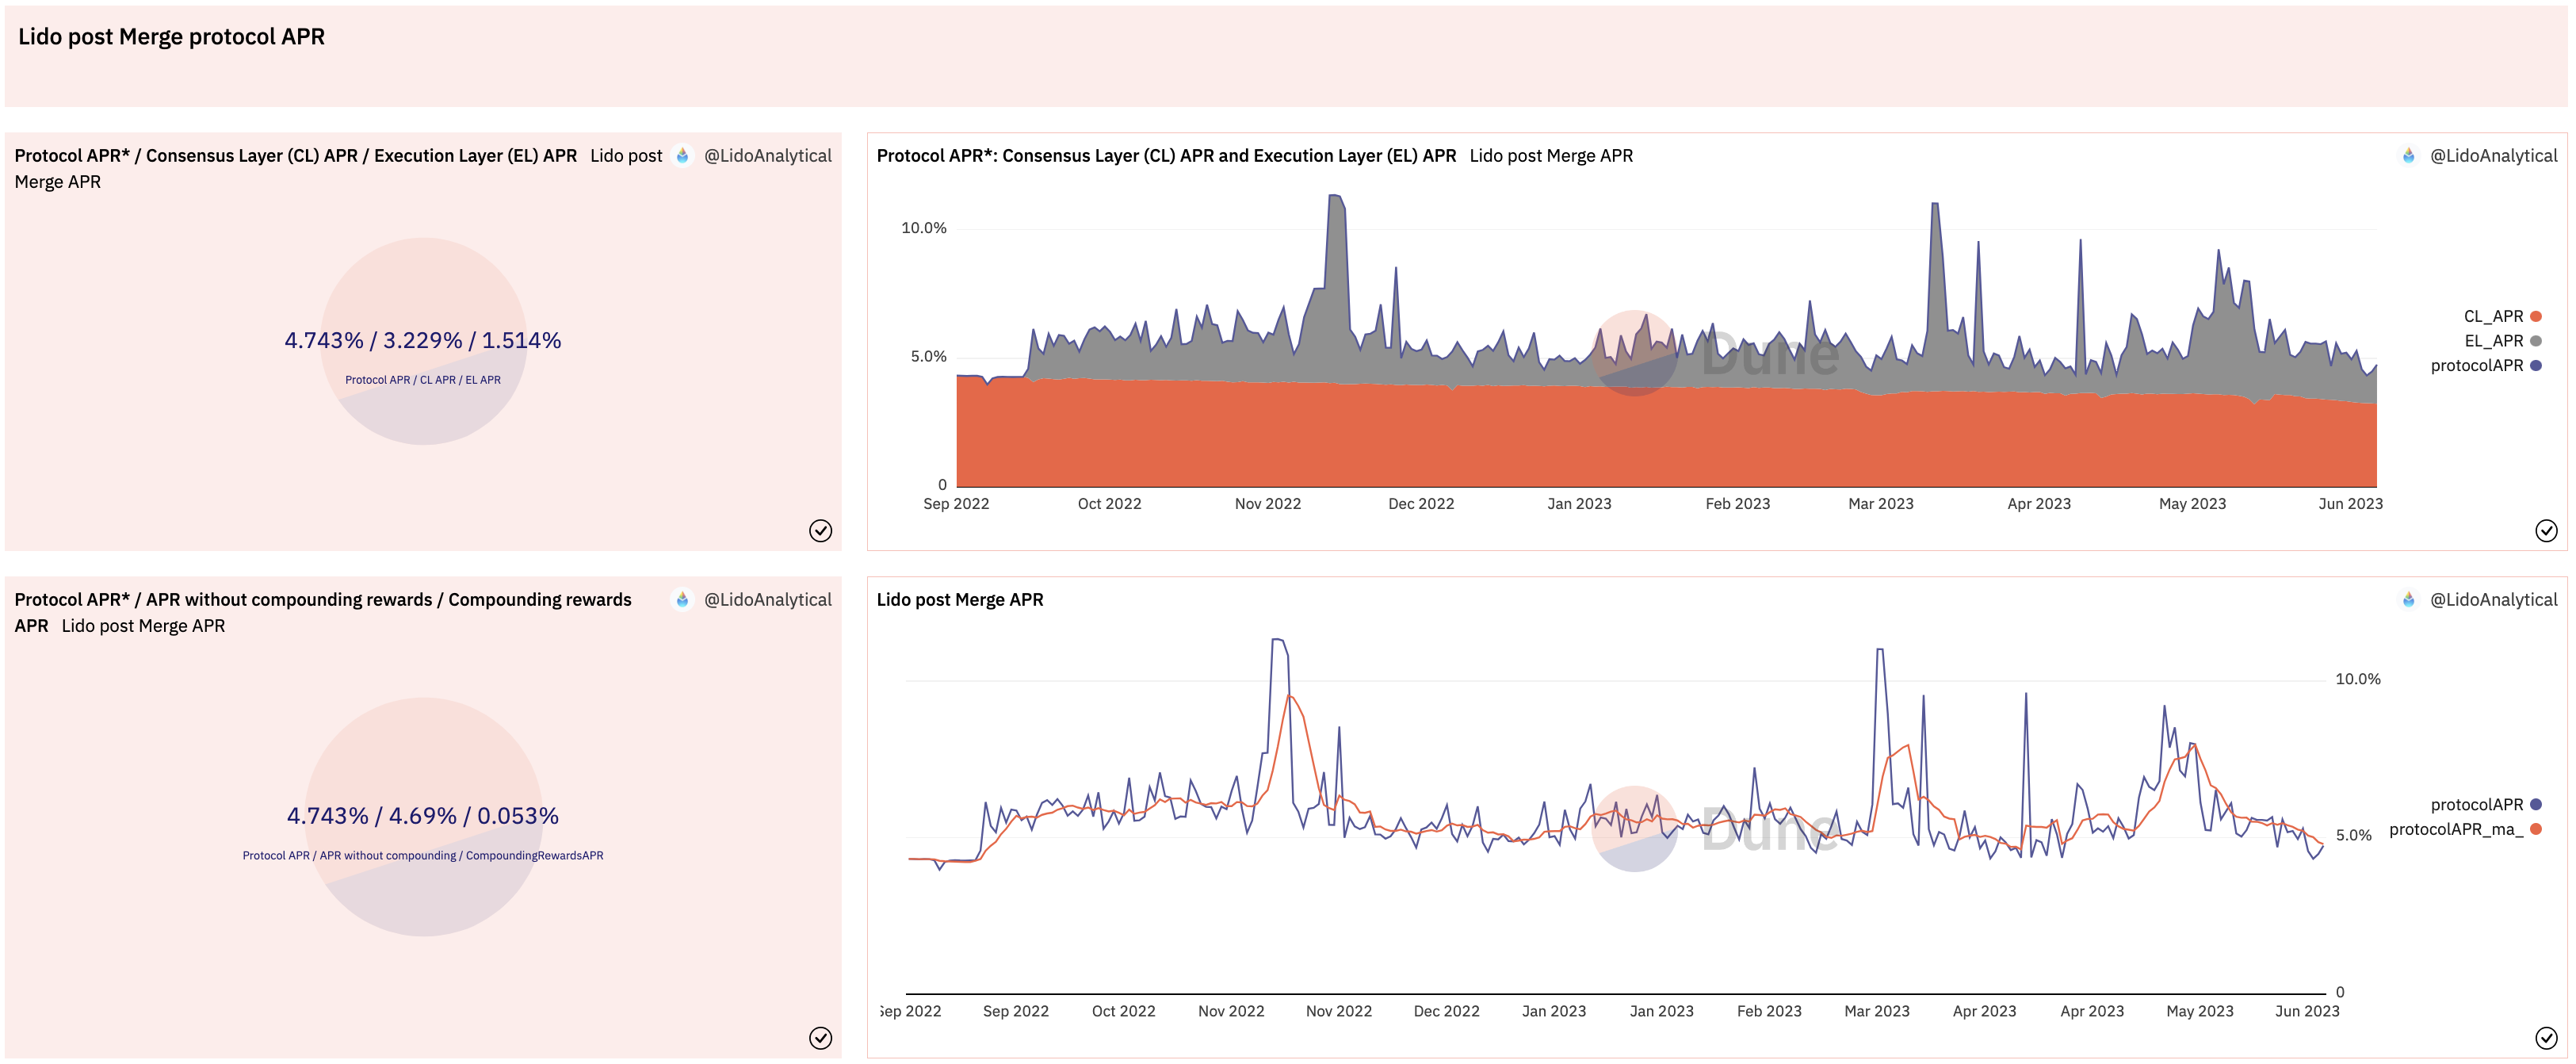
\includegraphics[width=\linewidth]{../images/dunelido1}\\
%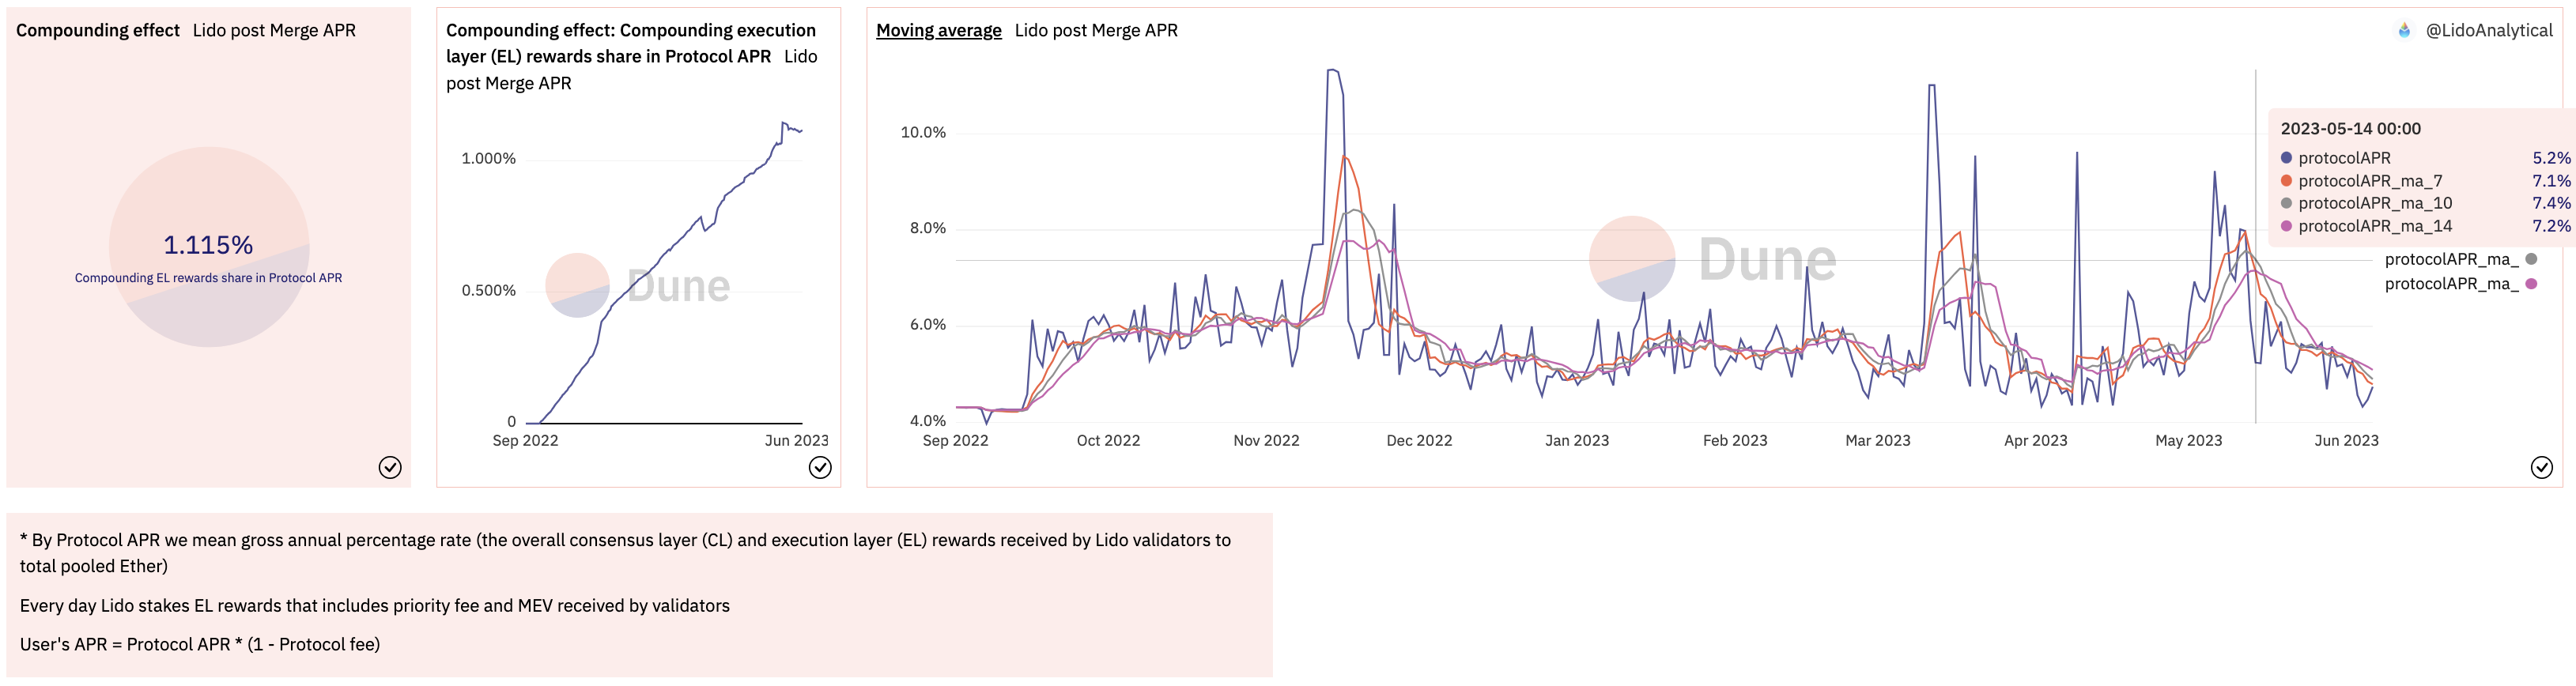
\includegraphics[width=\linewidth]{../images/dunelido2}
%\caption{Dune Analytics Lido post Merge protocol APR dashboard by @LidoAnalytical  (7 June 2023)}
%\label{fig:dunelido1}
%\end{center}
%\end{figure}
%
%\begin{figure}[htbp]
%\begin{center}
%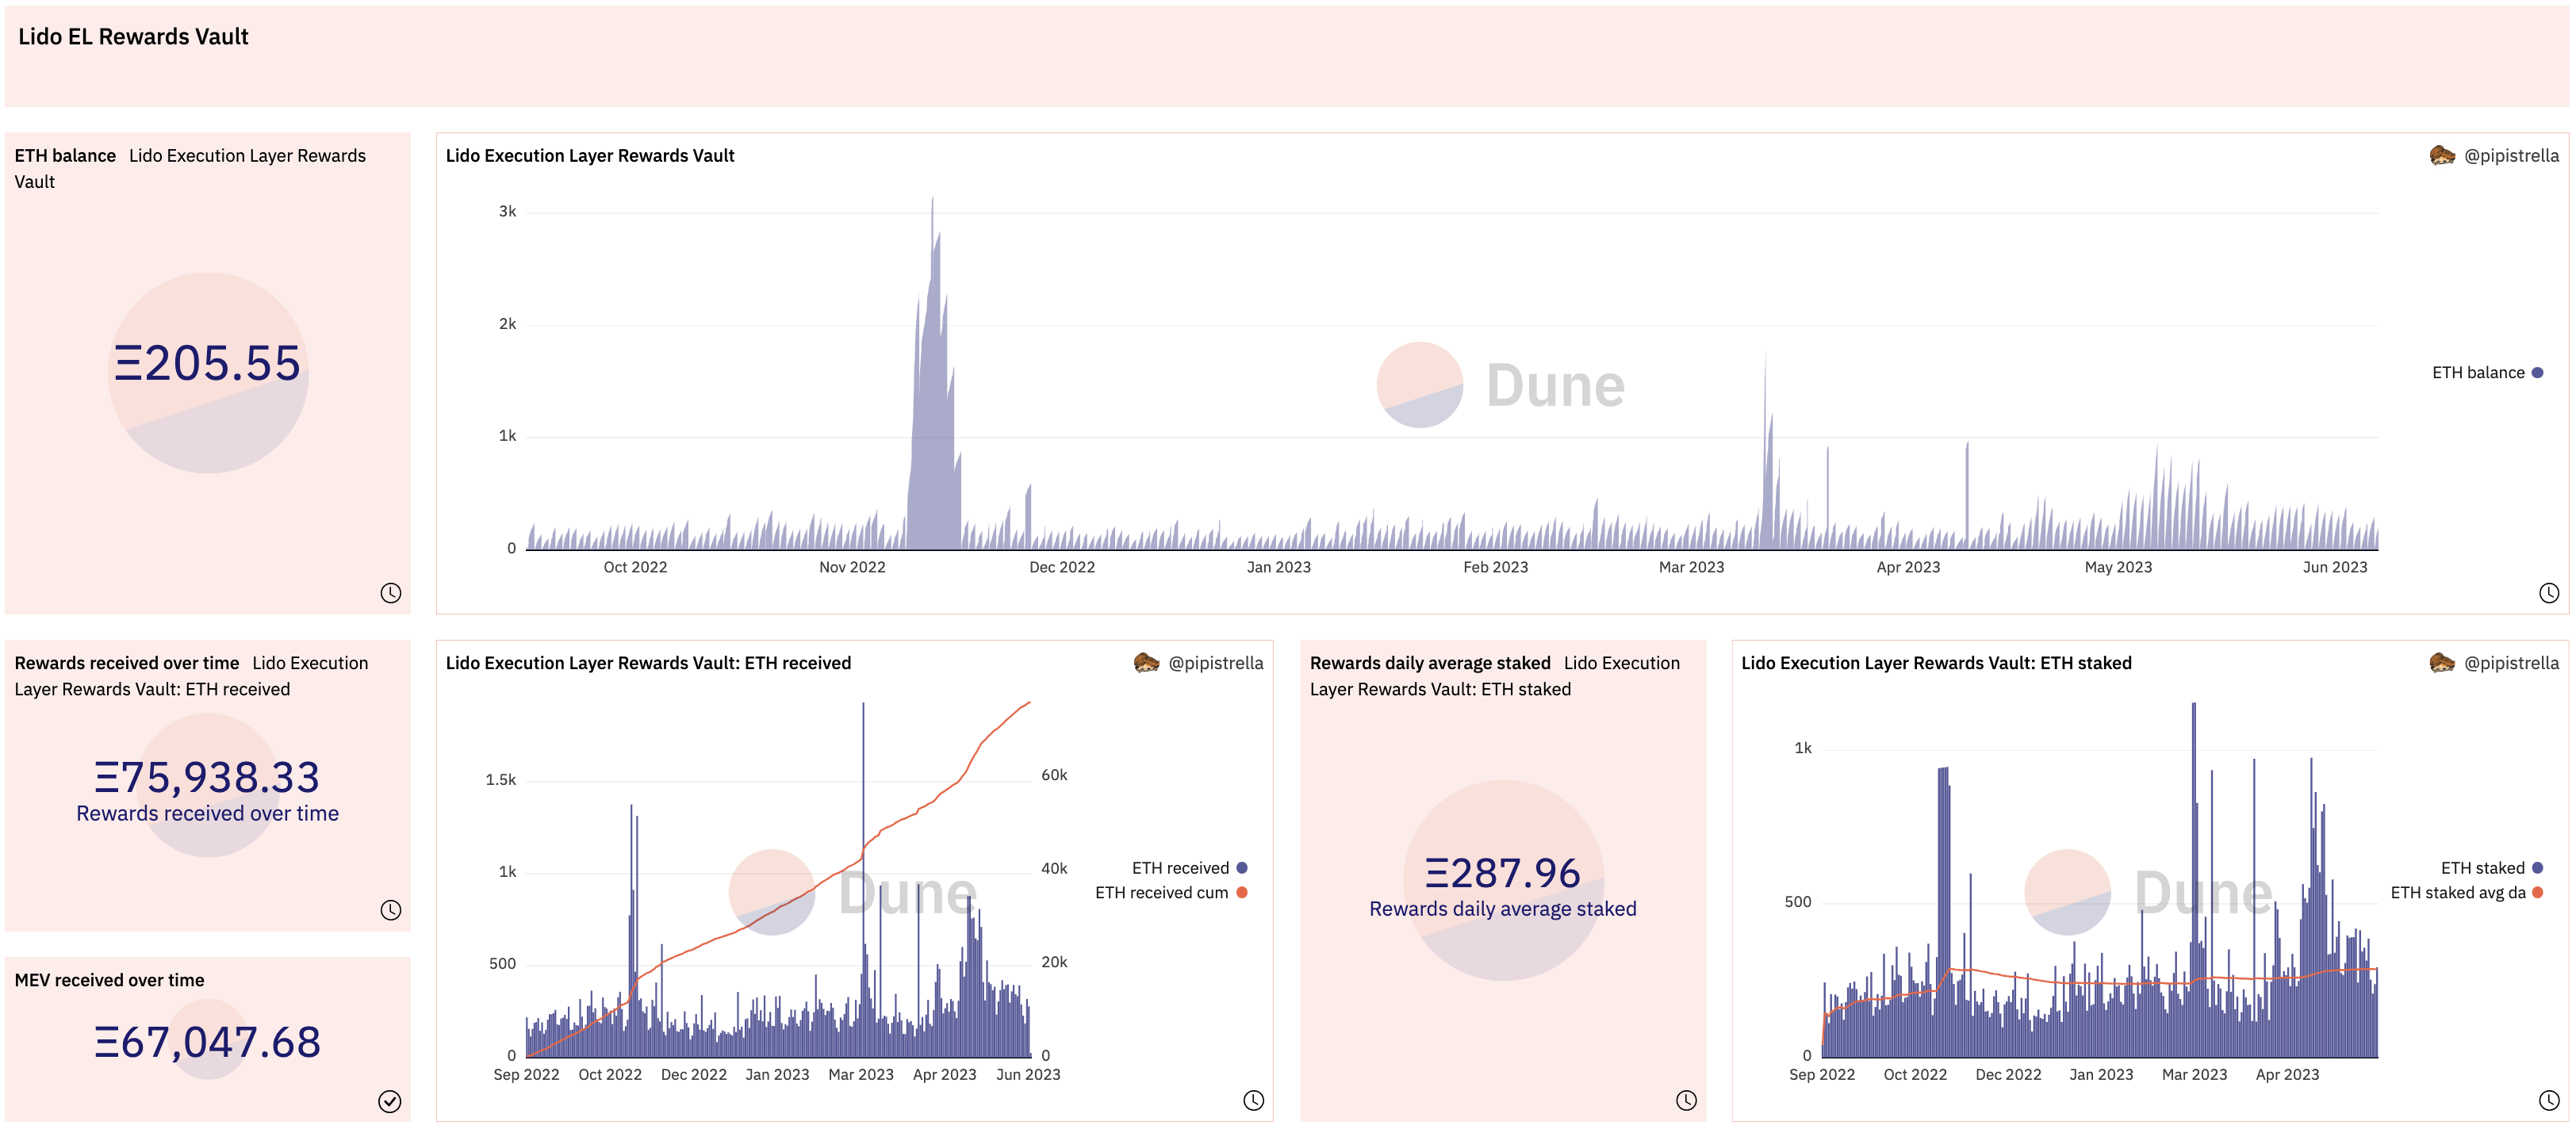
\includegraphics[width=\linewidth]{../images/dunelido3}
%\caption{Dune Analytics Lido Execution Layer rewards by @LidoAnalytical  (7 June 2023)}
%\label{fig:dunelido3}
%\end{center}
%\end{figure}
%
%\begin{figure}[htbp]
%\begin{center}
%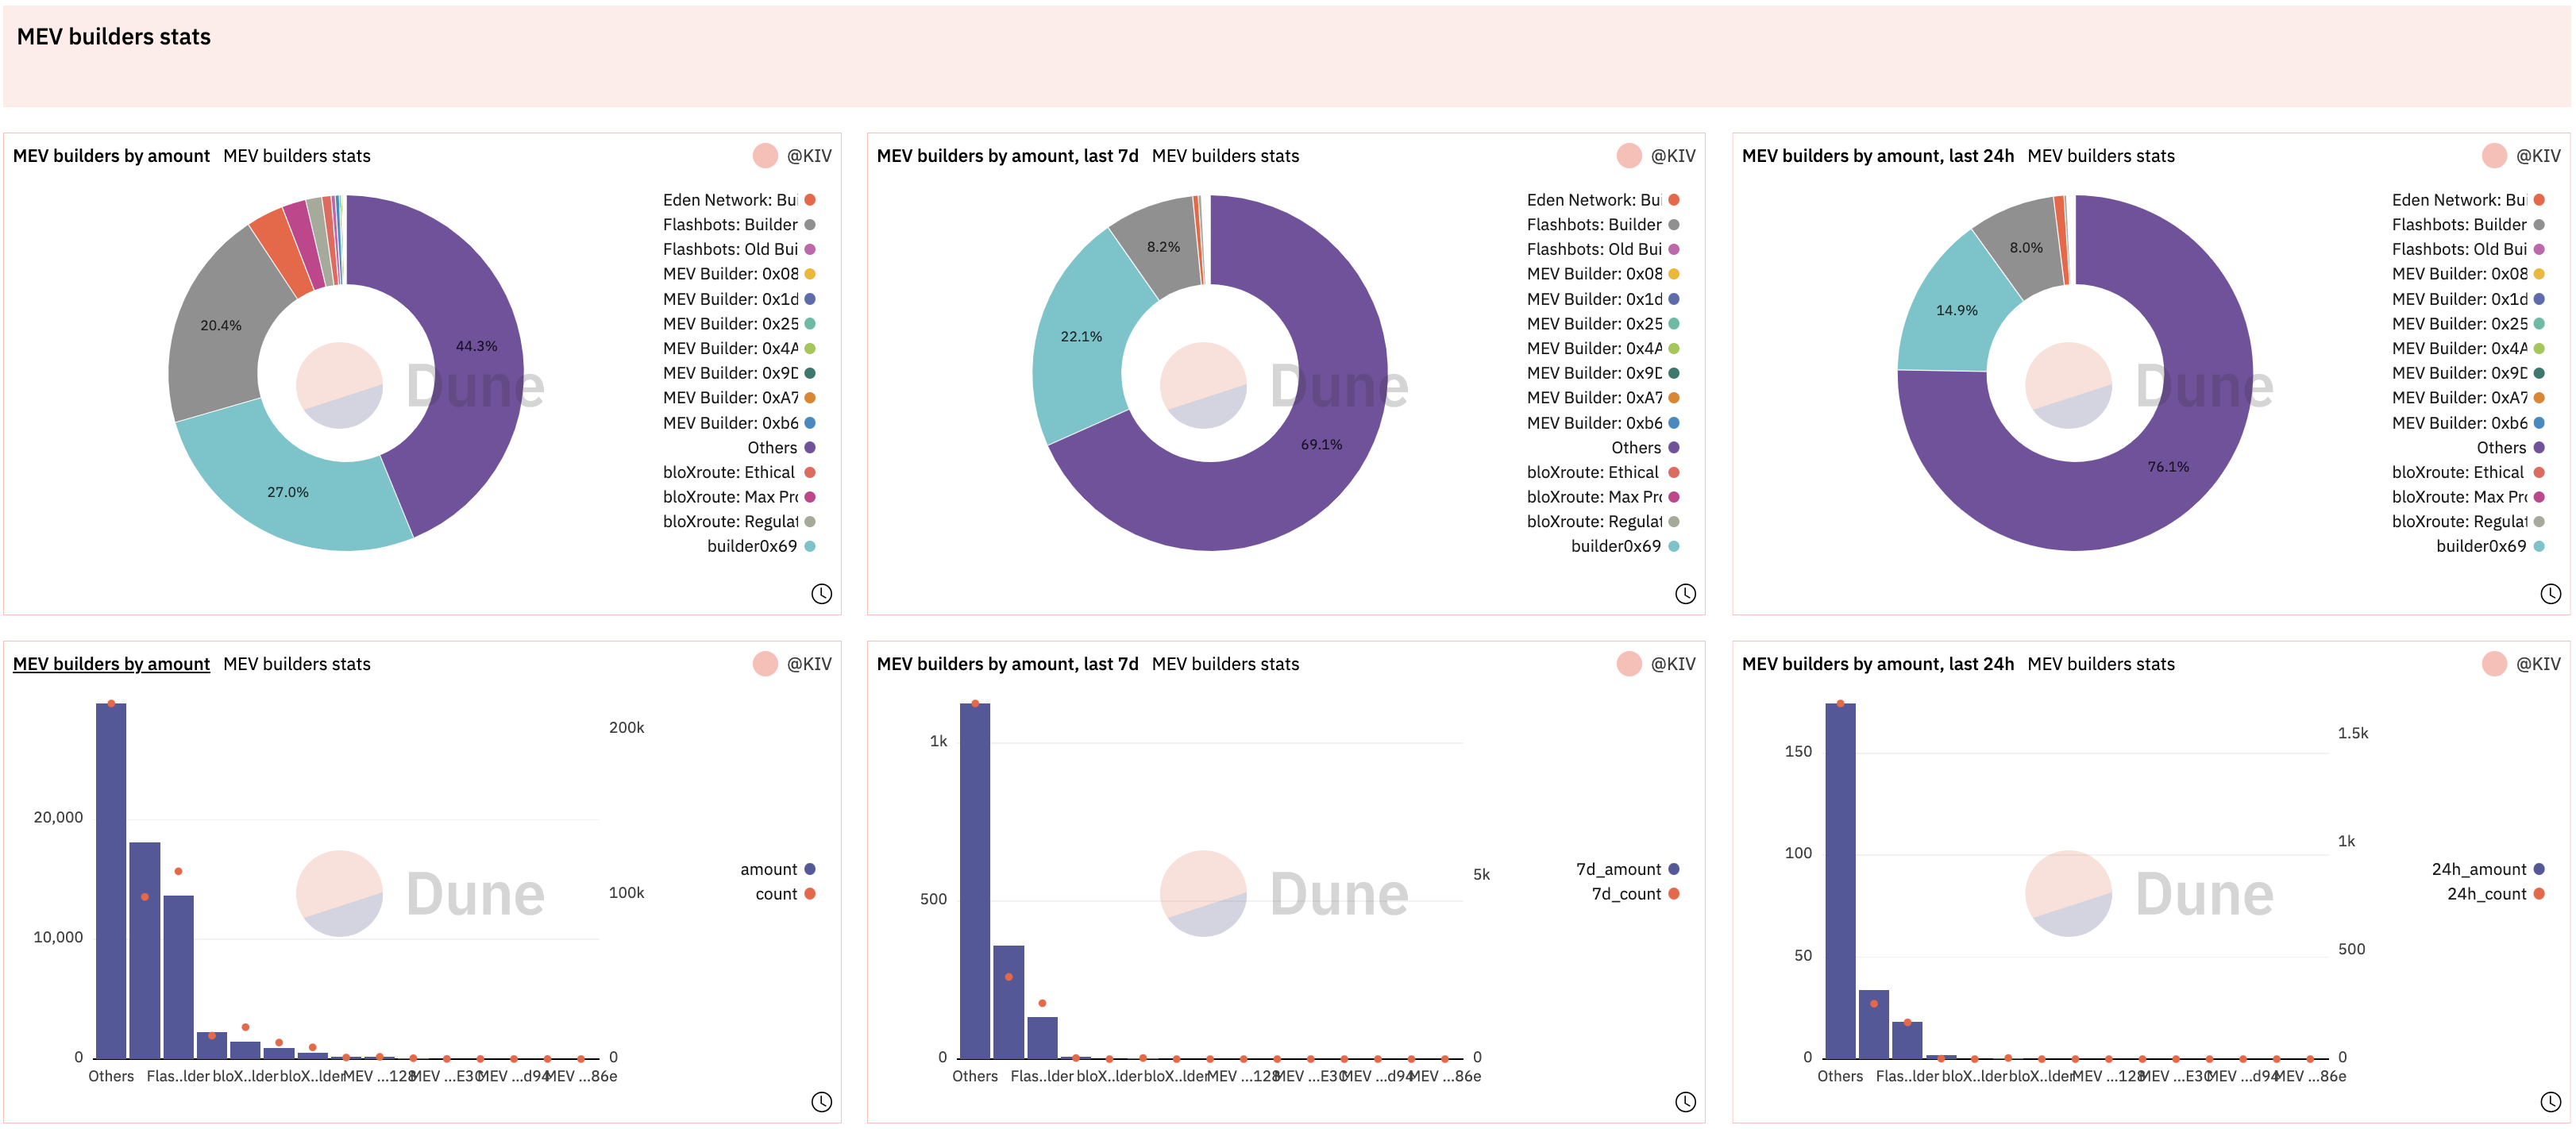
\includegraphics[width=\linewidth]{../images/dunelido4}\\
%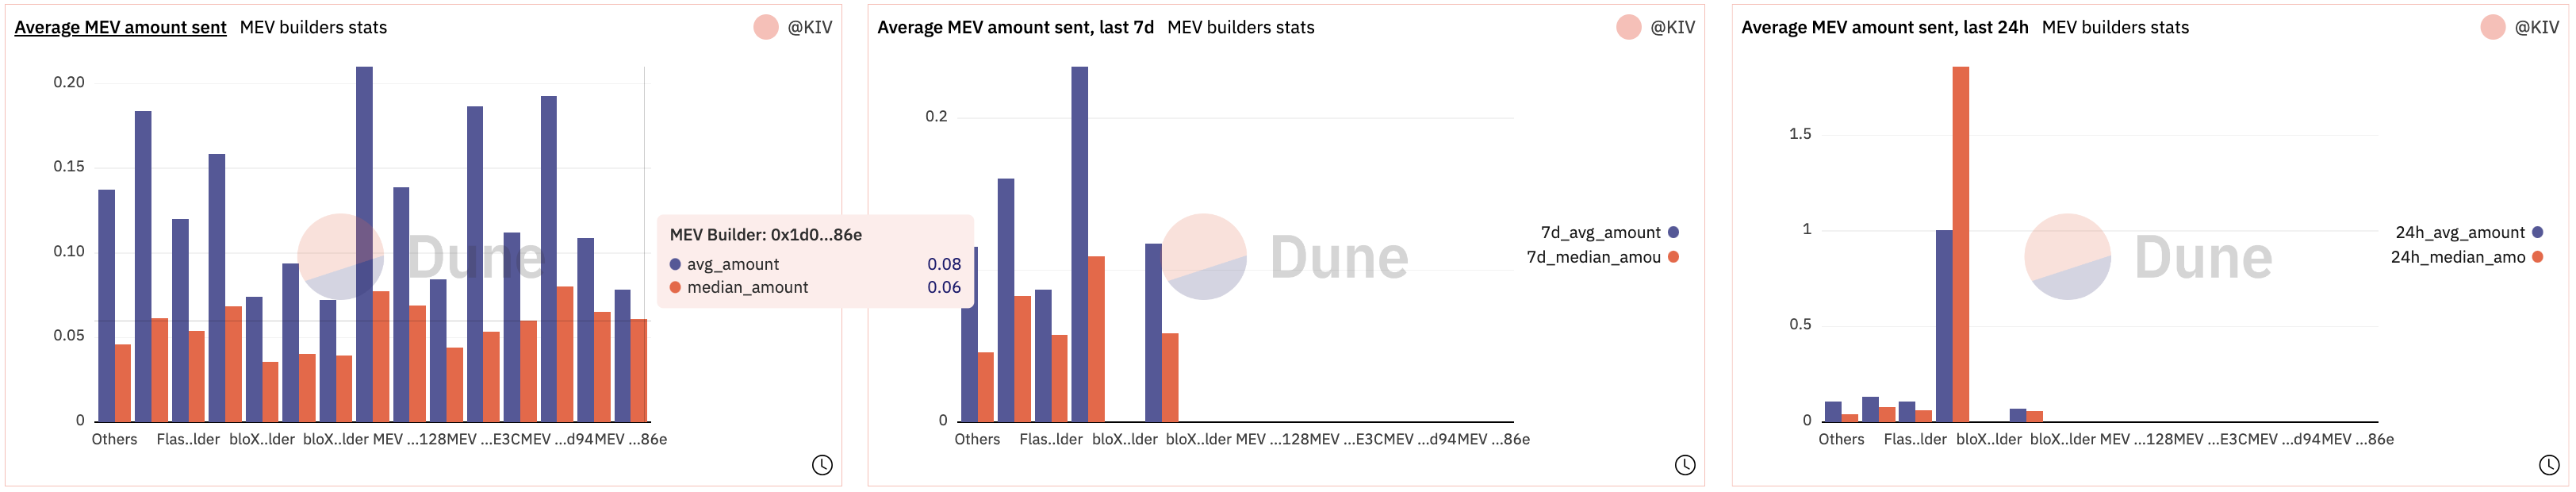
\includegraphics[width=\linewidth]{../images/dunelido5}
%\caption{Dune Analytics Lido MEV builders statistics by @LidoAnalytical  (7 June 2023)}
%\label{fig:dunelido5}
%\end{center}
%\end{figure}
%\noindent
%\clearpage
%\noindent


\subsubsection*{Rocket Pool}
% -----------------------------------
A \href{https://rocketpool.net/}{Rocket Pool} node only needs to stake 16 ETH,
and this stake is then coupled with 16 ETH from the staking pool to create a
validator, known as a ``minipool''.  Staking in the Rocket Pool can be a stake
of a little as 0.01 ETH, which is then issued as an rETH token representing the
amount deposited into the pool. A node operator would obtain staked ETH from
the pool to form a validator.

There is documentation at the Rocket Pool website that clearly explains
Ethereum staking and how it works when staking with Rocket Pool.

Currently, 8 June 2023, Rocket Pool has staked 722,176 ETH and has 2,842 node
operators.

If we can identify the number of distinct rETH token holders, we would be able
to determine the number of stakers staking ETH in Rocket Pool. 

%
%Examples of the graphs and information available from the Dune dashboard are shown in figures~\ref{fig:dunerocket1}~-~\ref{fig:rocketdrworm12} on pages~\pageref{fig:dunerocket1}~-~\pageref{fig:rocketdrworm12}.
%
% \textbf{Dune Analytics}
%% -------------
%\textbf{Rocket Pool}
%% -------------
%\begin{figure}[htbp]
%\begin{center}
%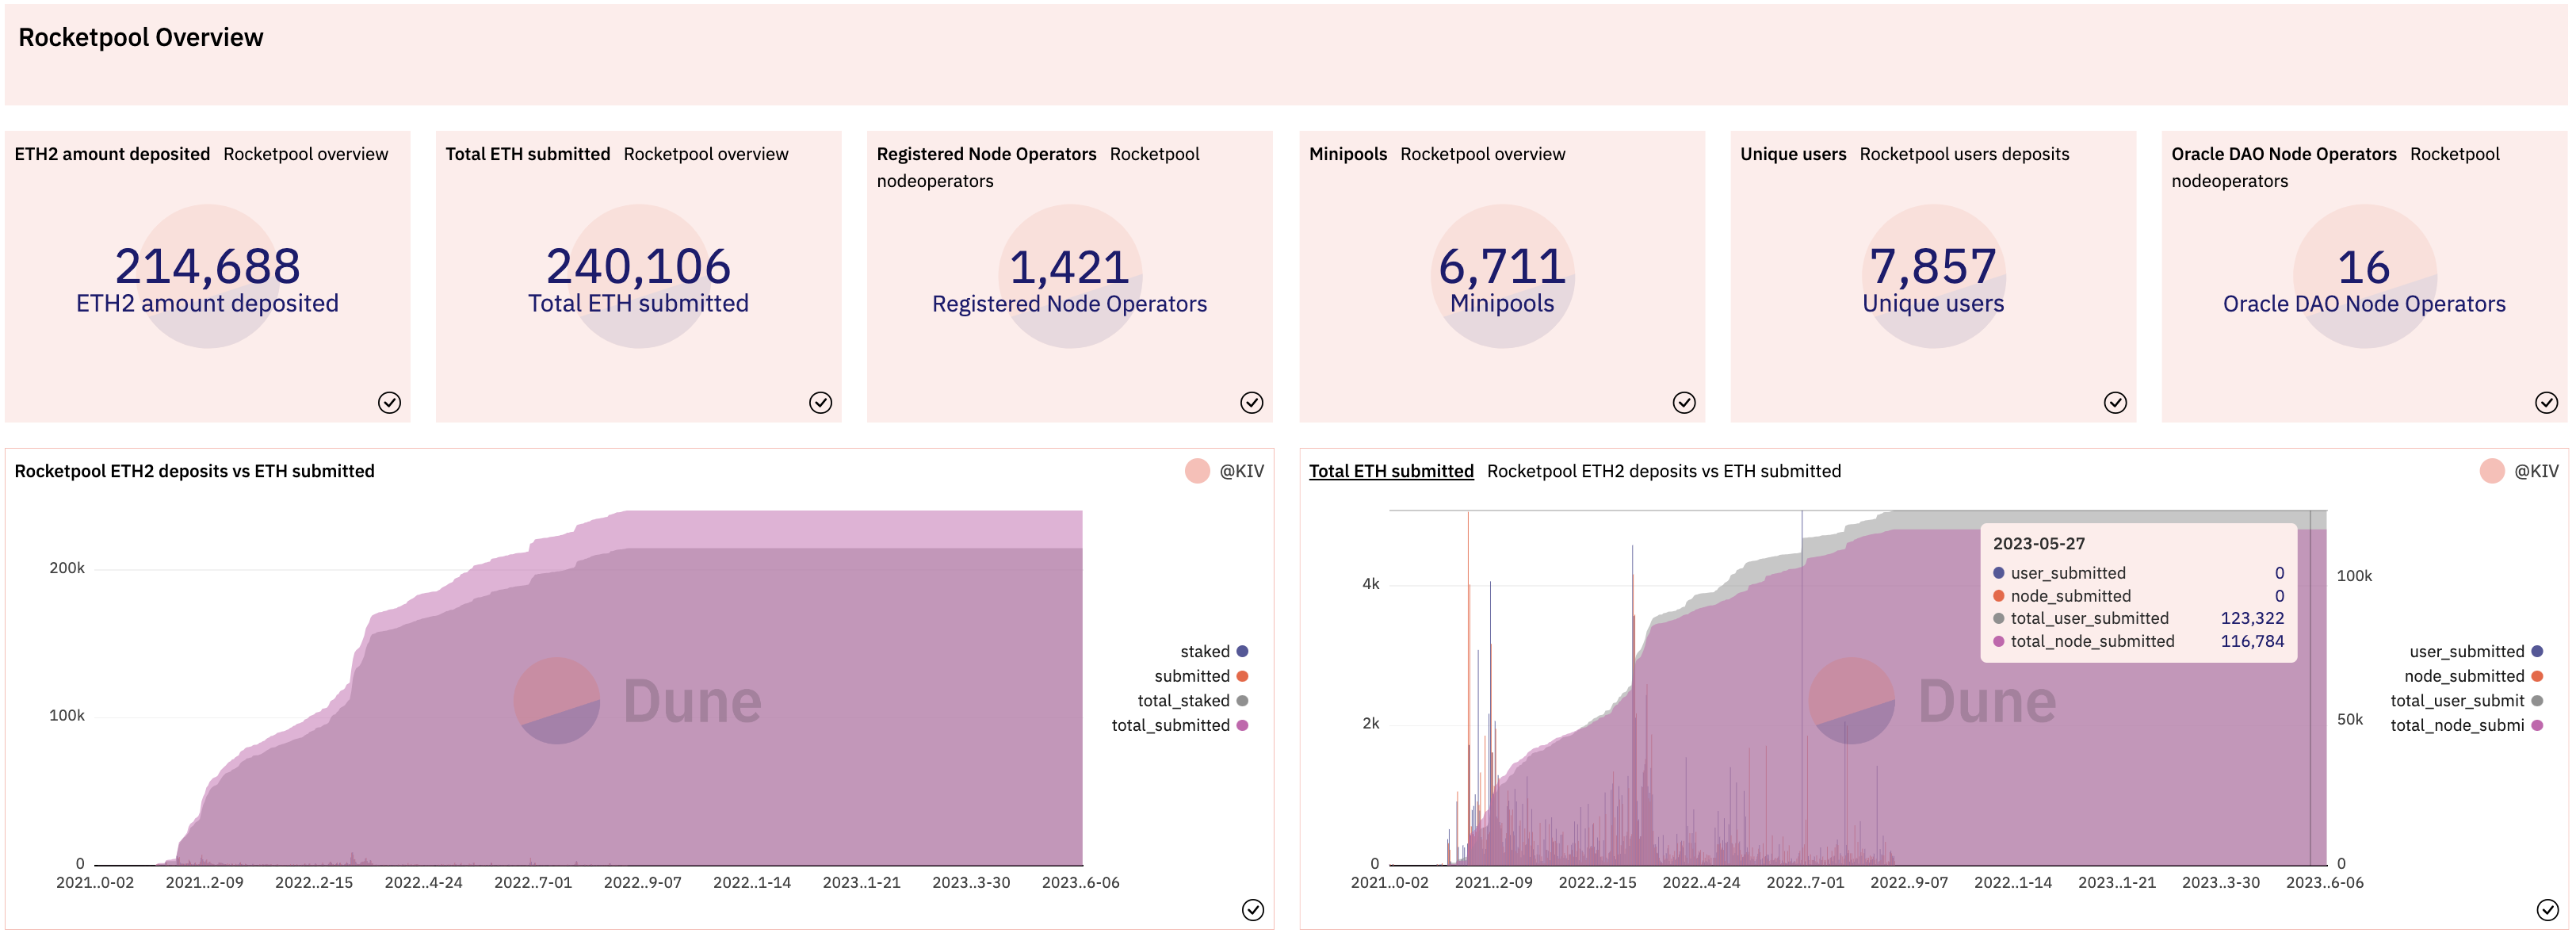
\includegraphics[width=\linewidth]{../images/dunerocket1}\\
%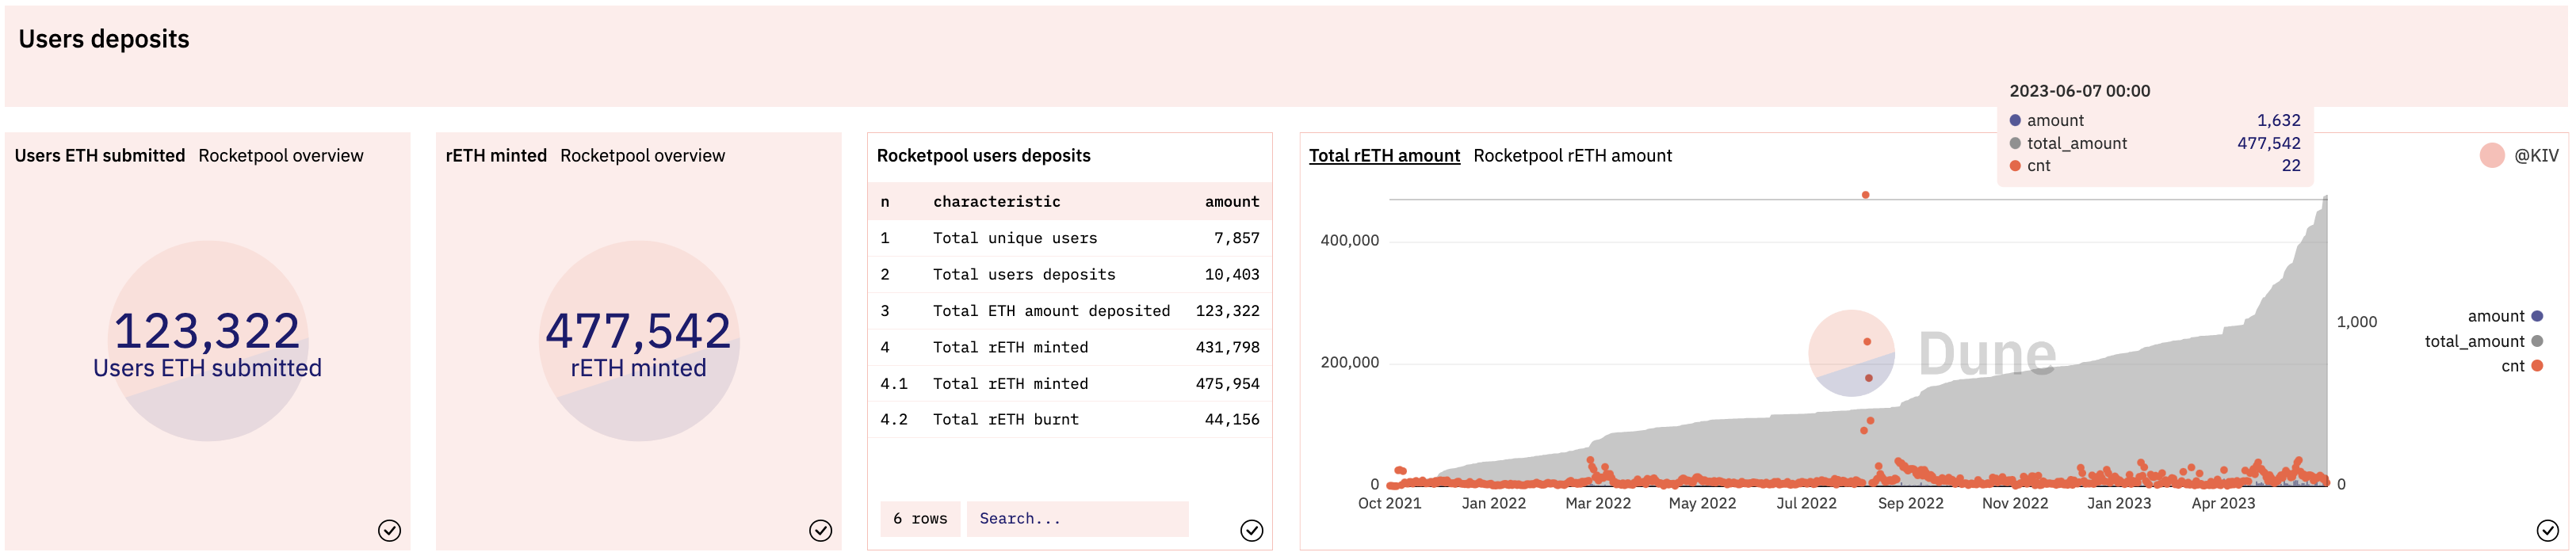
\includegraphics[width=\linewidth]{../images/dunerocket2}
%\caption{Dune Analytics Rocket Pool overview by @KIV  (7 June 2023)}
%\label{fig:dunerocket1}
%\end{center}
%\end{figure}
%
%\begin{figure}[htbp]
%\begin{center}
%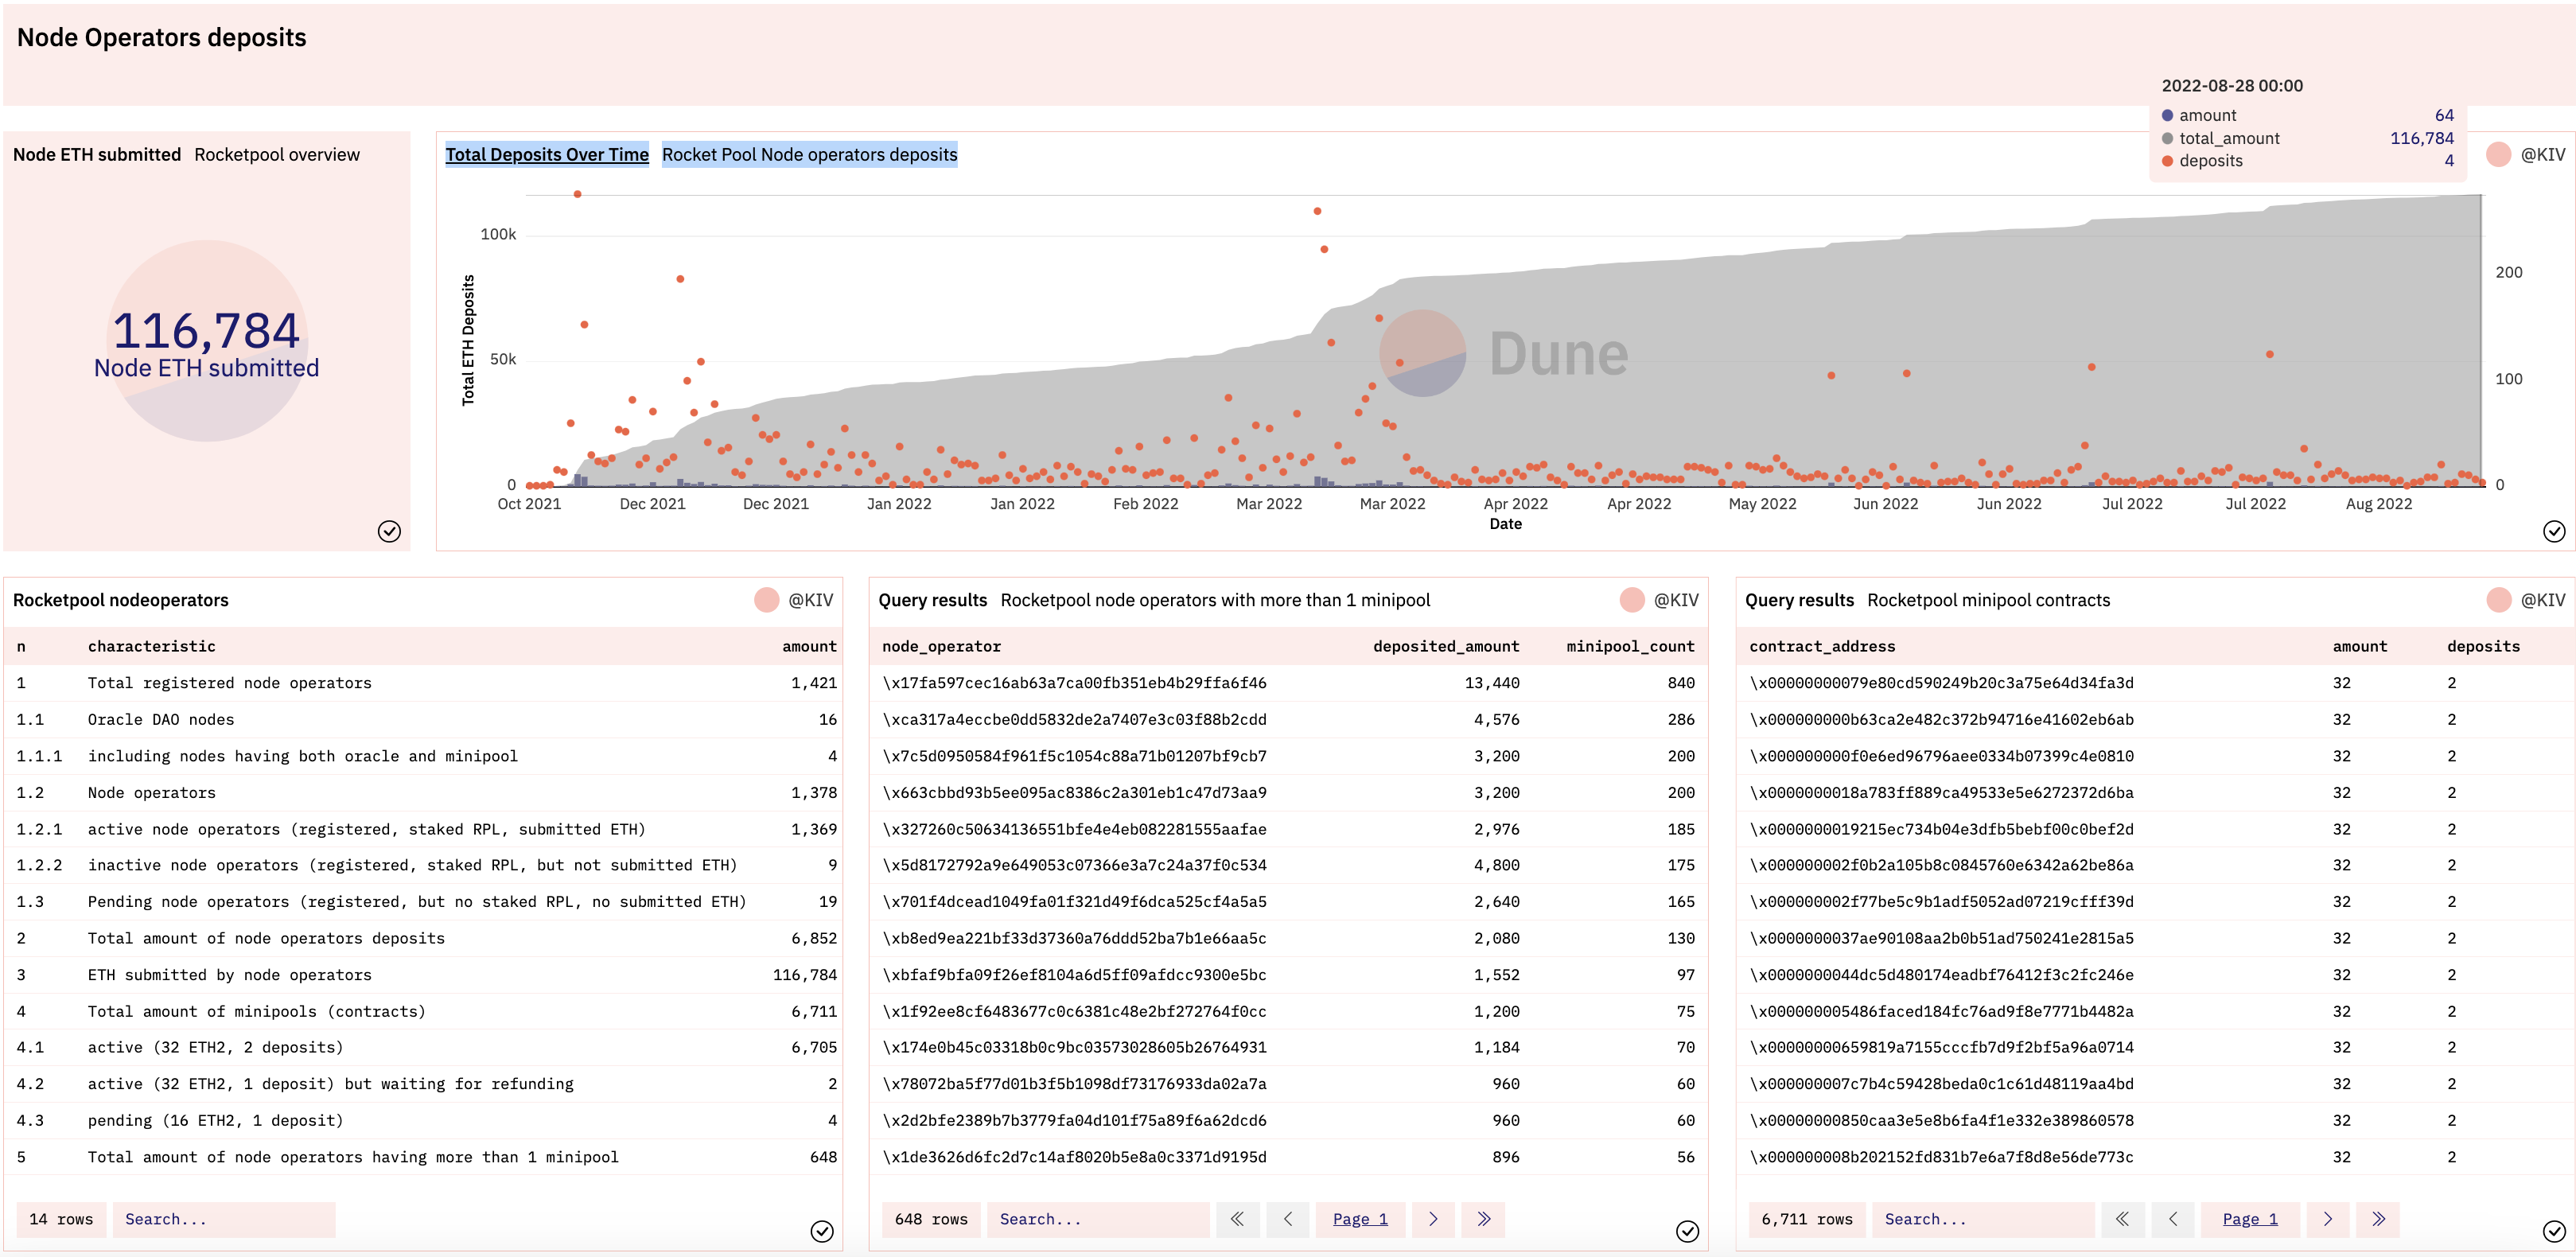
\includegraphics[width=\linewidth]{../images/dunerocket3}
%\caption{Dune Analytics Rocket Pool node operator deposits by @KIV  (7 June 2023)}
%\label{fig:dunerocket3}
%\end{center}
%\end{figure}
%
%\begin{figure}[htbp]
%\begin{center}
%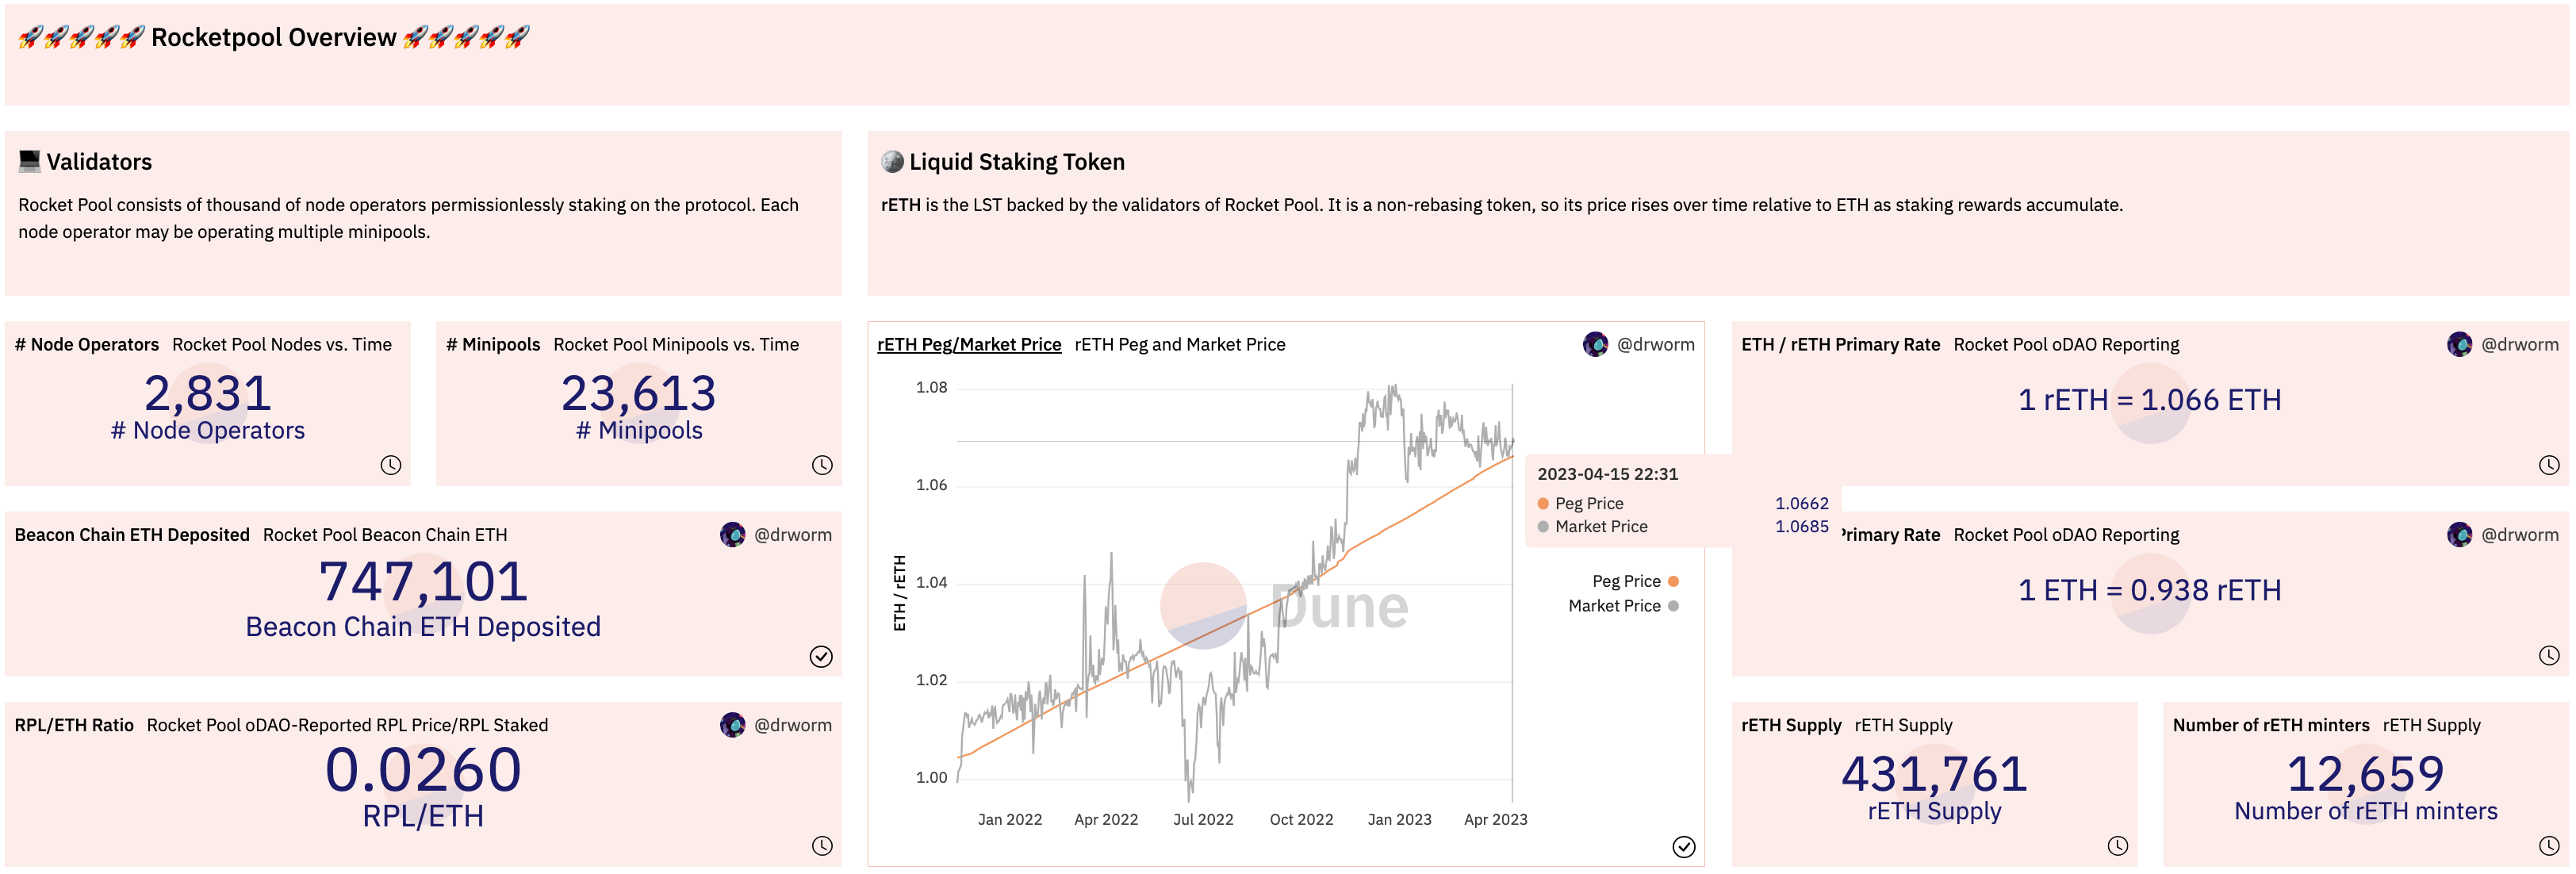
\includegraphics[width=\linewidth]{../images/rocketdrworm1}
%\caption{Dune Analytics Rocket Pool overview by @drworm  (7 June 2023)}
%\label{fig:rocketdrworm1}
%\end{center}
%\end{figure}
%
%\begin{figure}[htbp]
%\begin{center}
%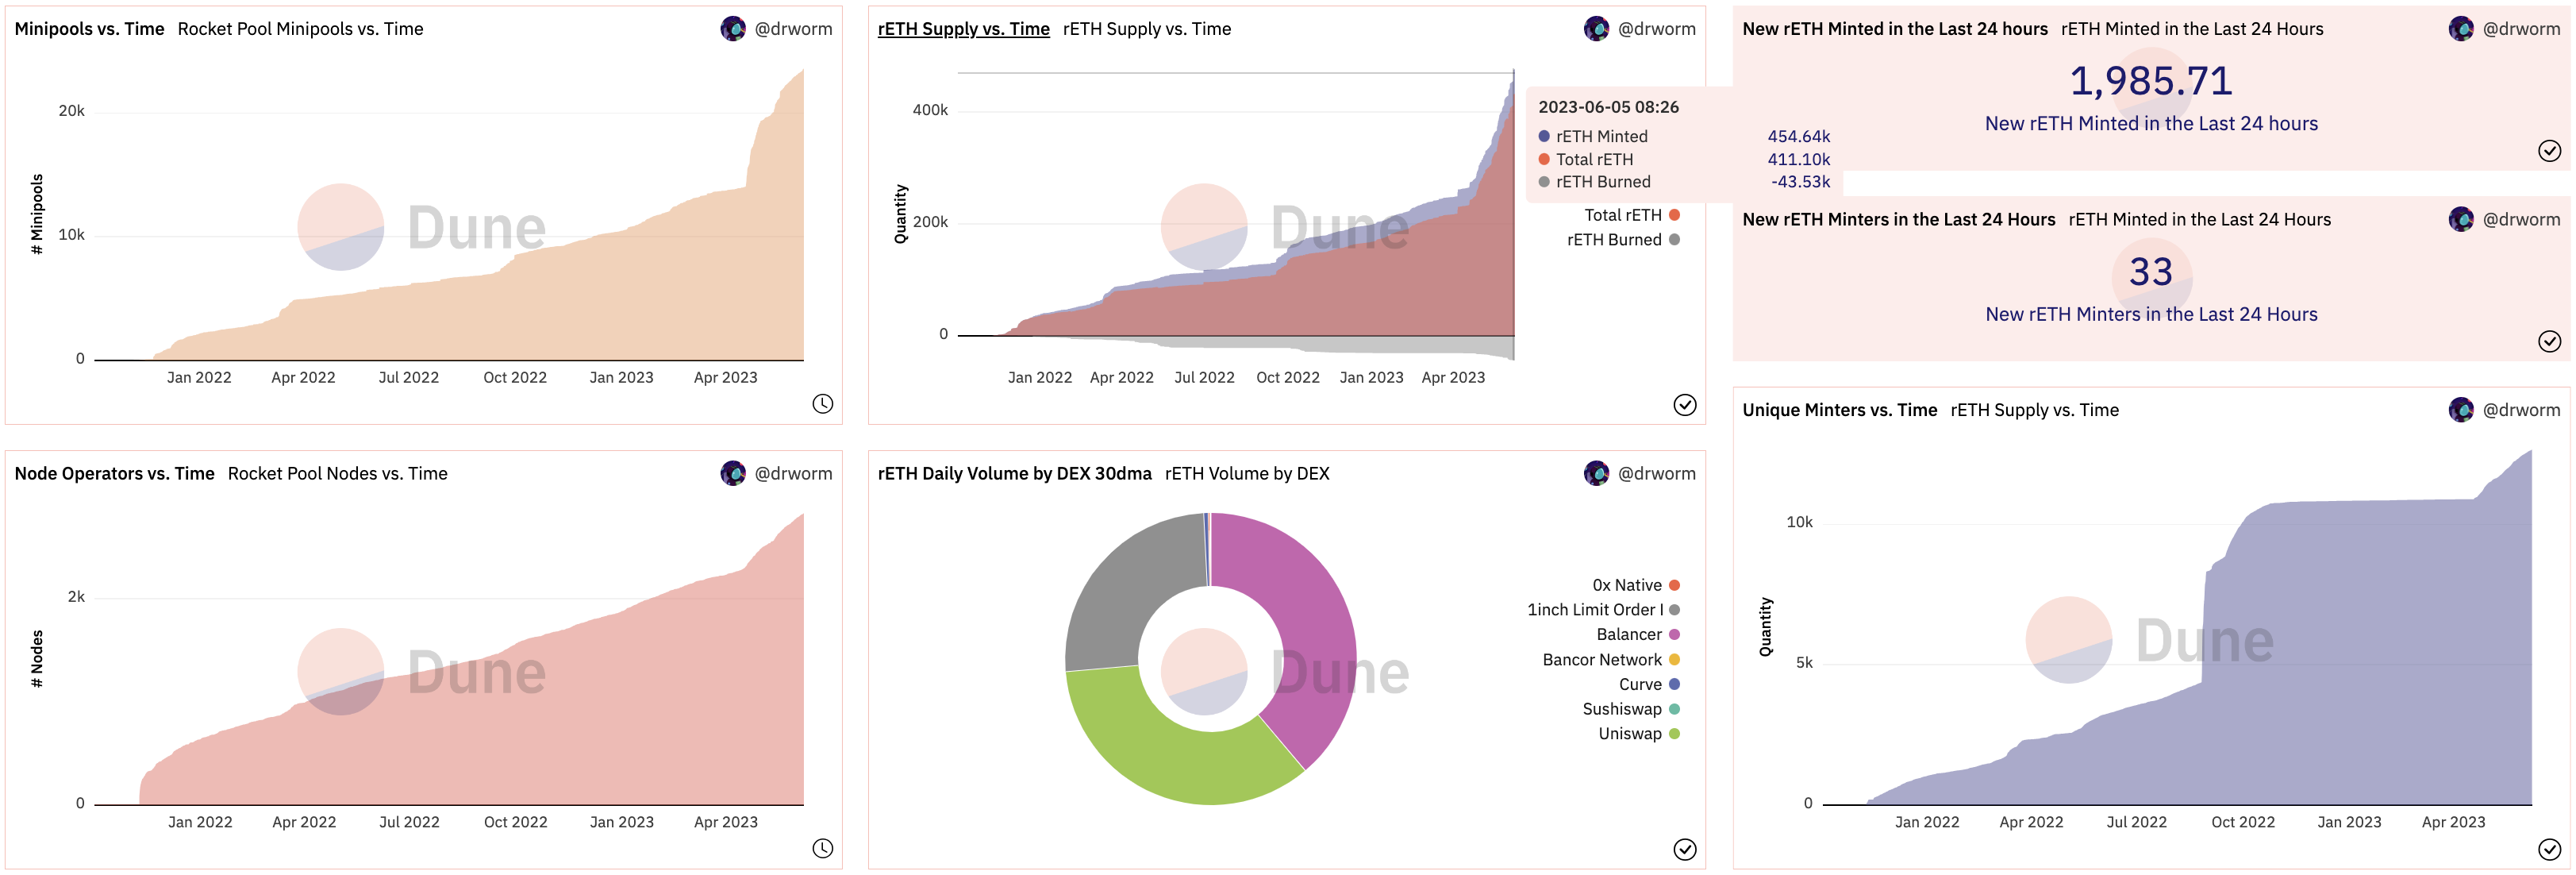
\includegraphics[width=\linewidth]{../images/rocketdrworm2}
%\caption{Dune Analytics Rocket Pool various statistics by @drworm  (7 June 2023)}
%\label{fig:rocketdrworm2}
%\end{center}
%\end{figure}
%
%\begin{figure}[htbp]
%\begin{center}
%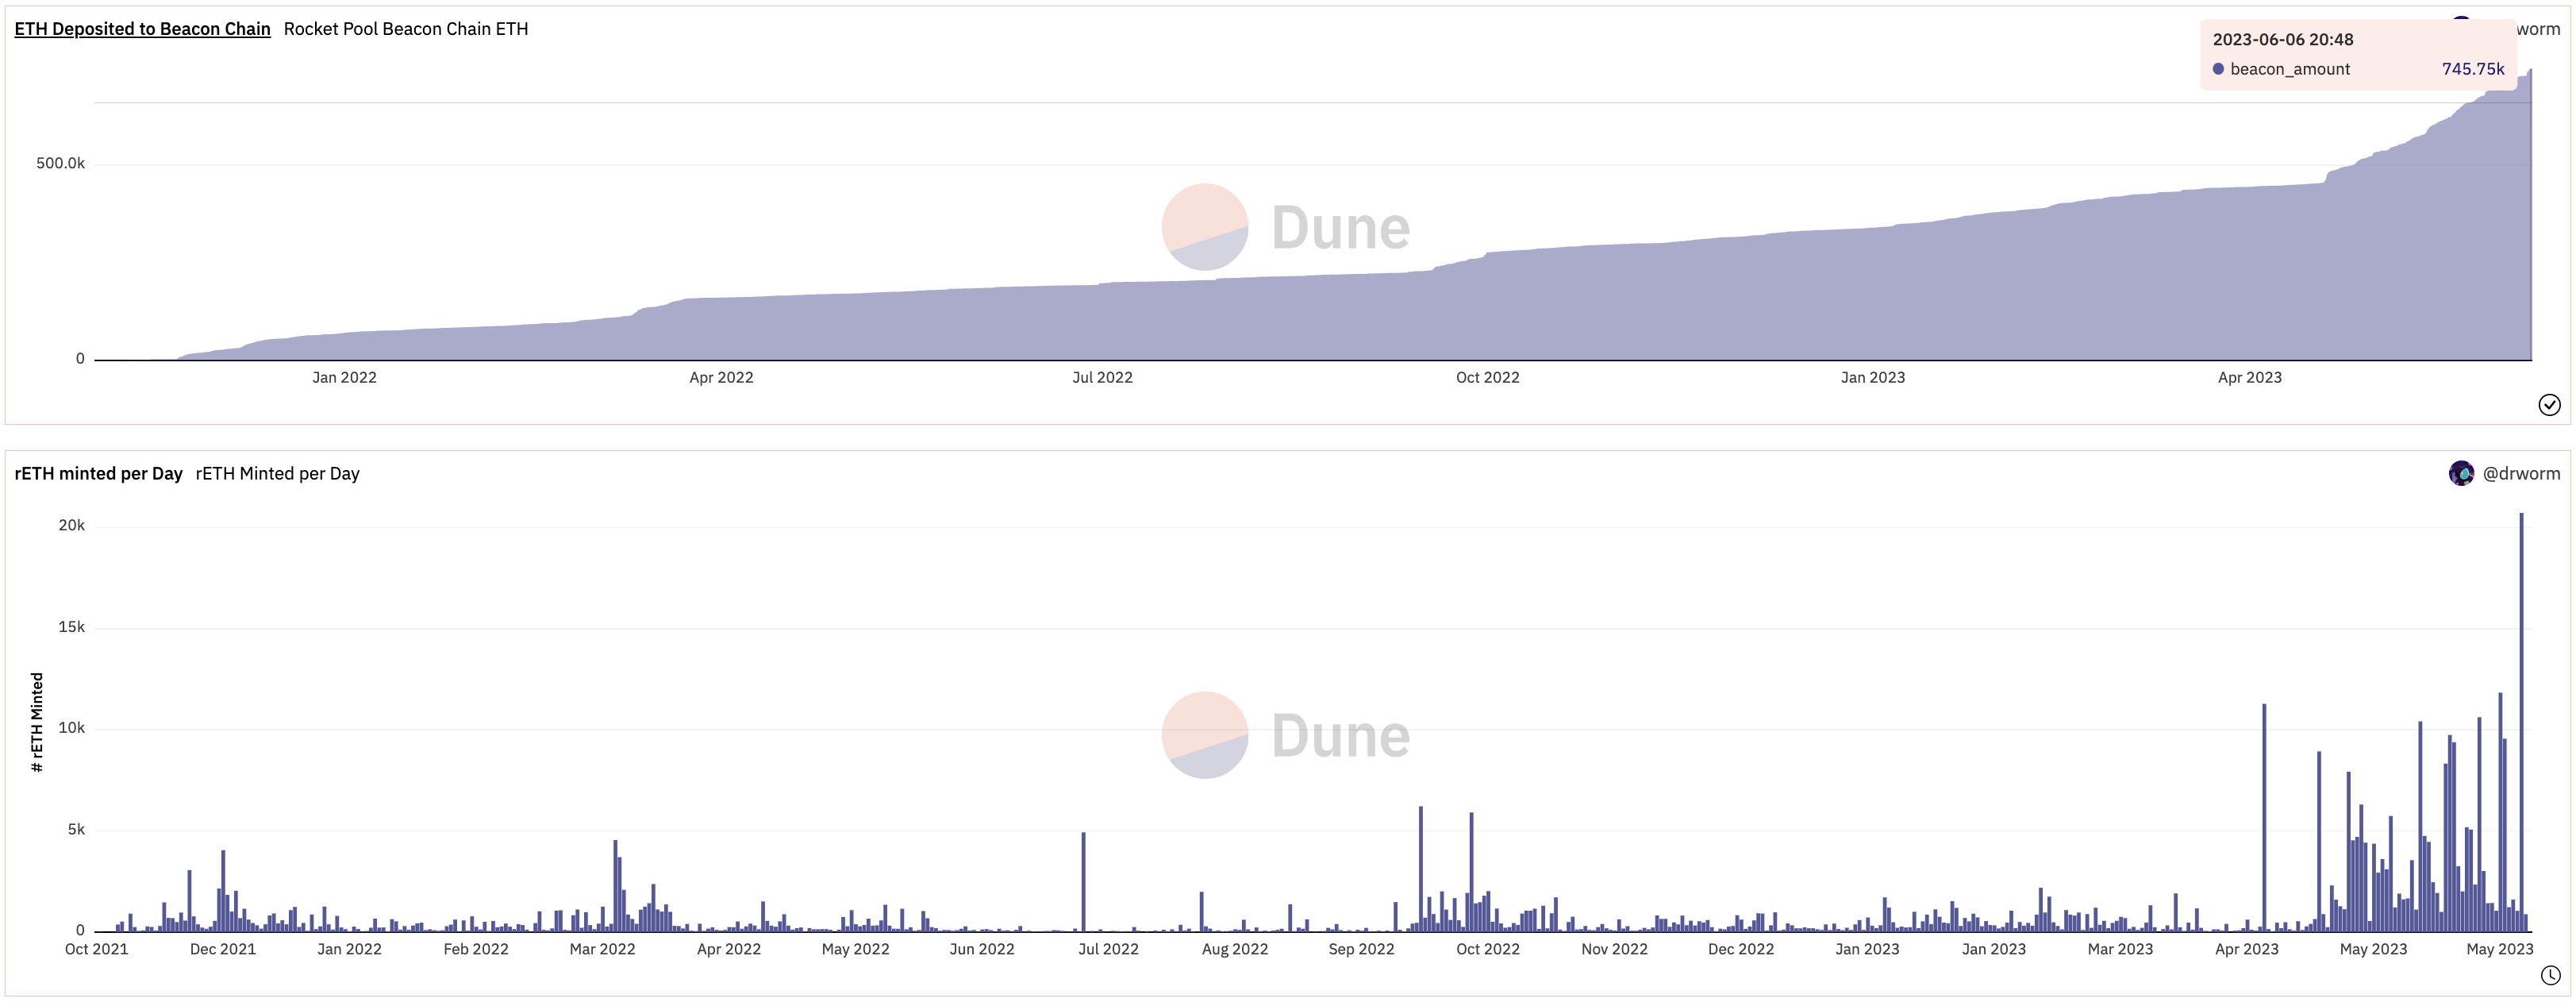
\includegraphics[width=\linewidth]{../images/rocketdrworm3}
%\caption{Dune Analytics Rocket Pool ETH deposited \& rETH minted by @drworm  (7 June 2023)}
%\label{fig:rocketdrworm3}
%\end{center}
%\end{figure}
%
%
%\begin{figure}[htbp]
%\begin{center}
%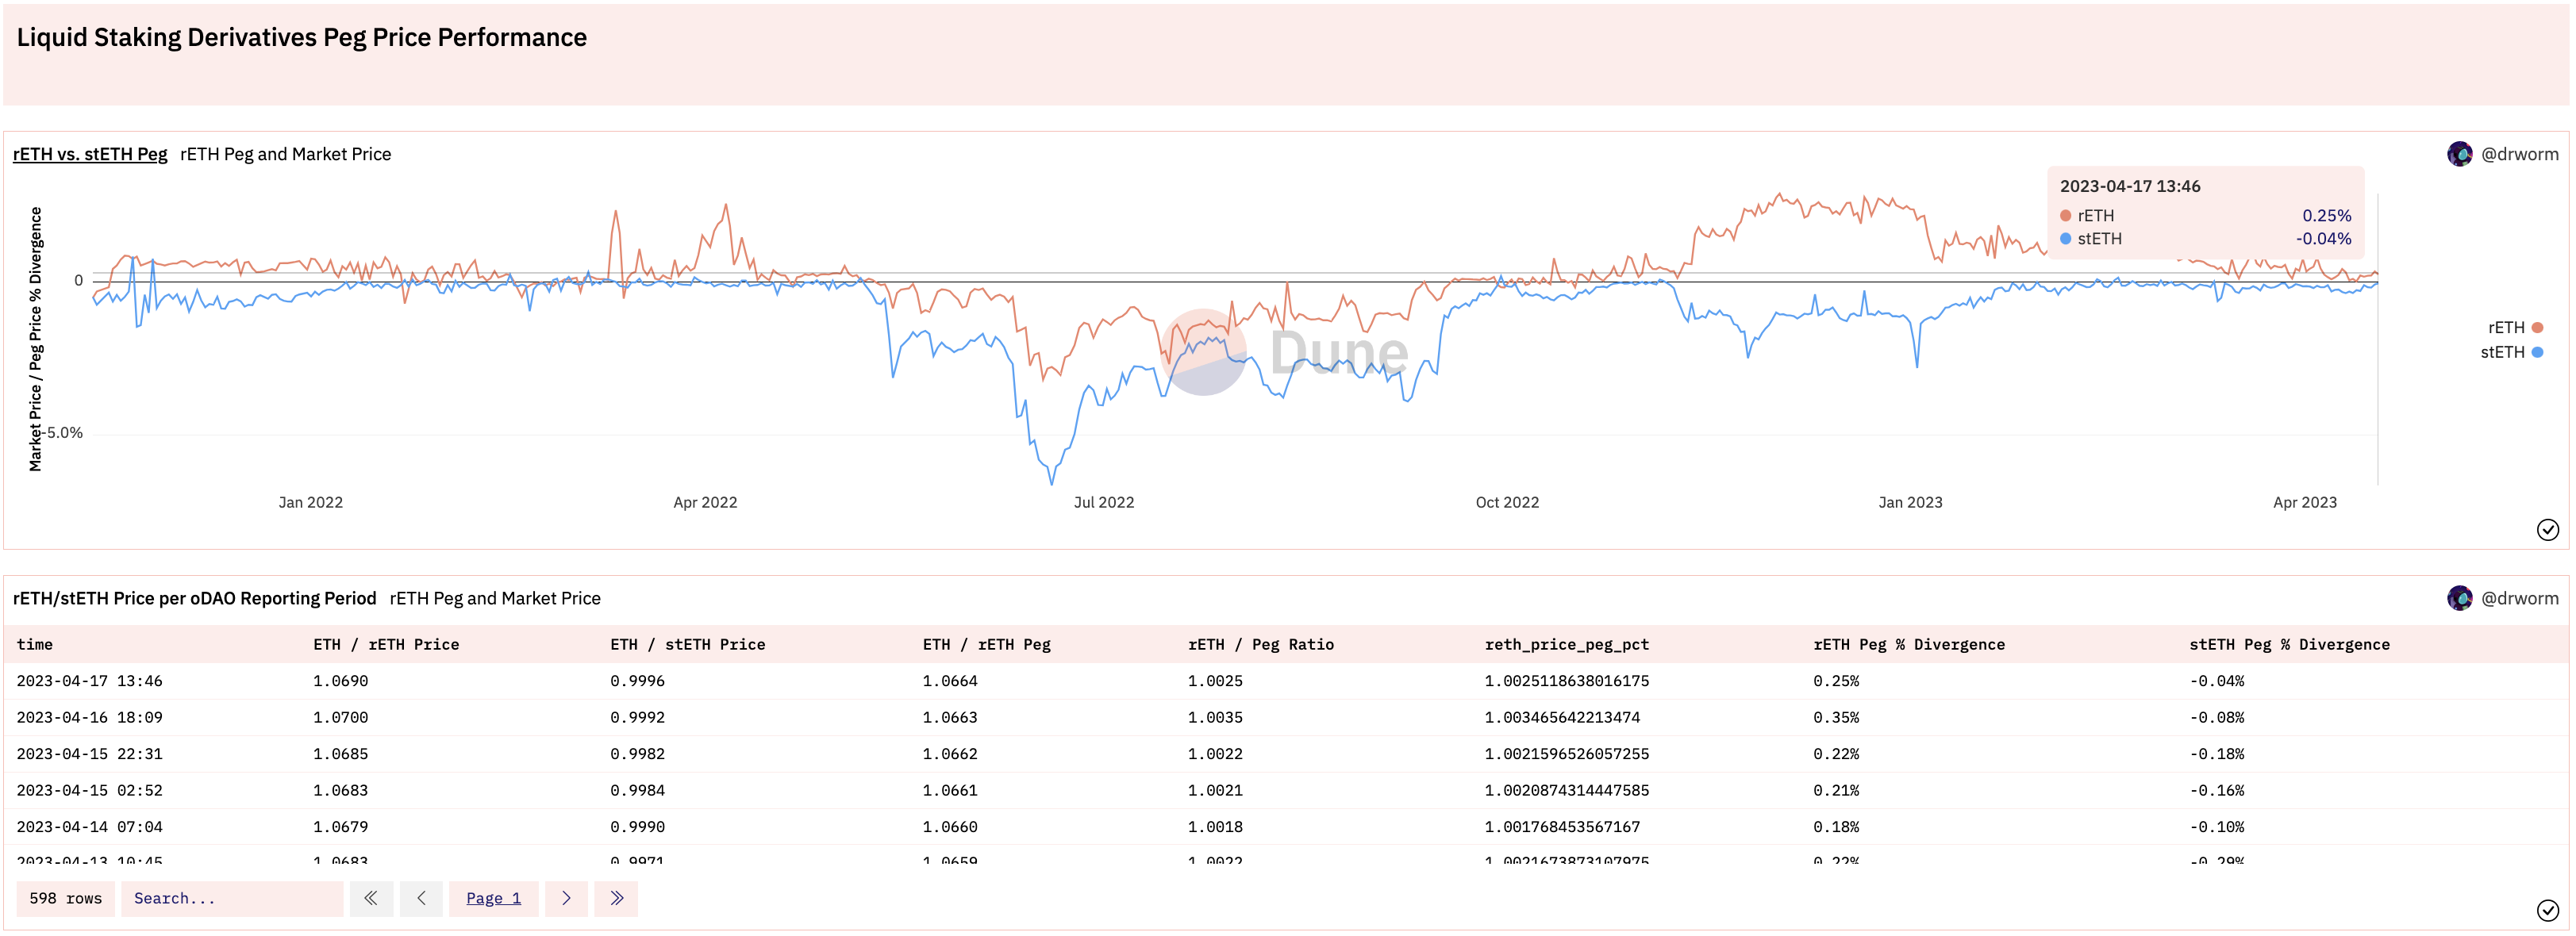
\includegraphics[width=\linewidth]{../images/rocketdrworm4}
%\caption{Dune Analytics Rocket Pool liquid staking derivatives peg price performance by @worm  (7 June 2023)}
%\label{fig:rocketdrworm4}
%\end{center}
%\end{figure}
%
%\begin{figure}[htbp]
%\begin{center}
%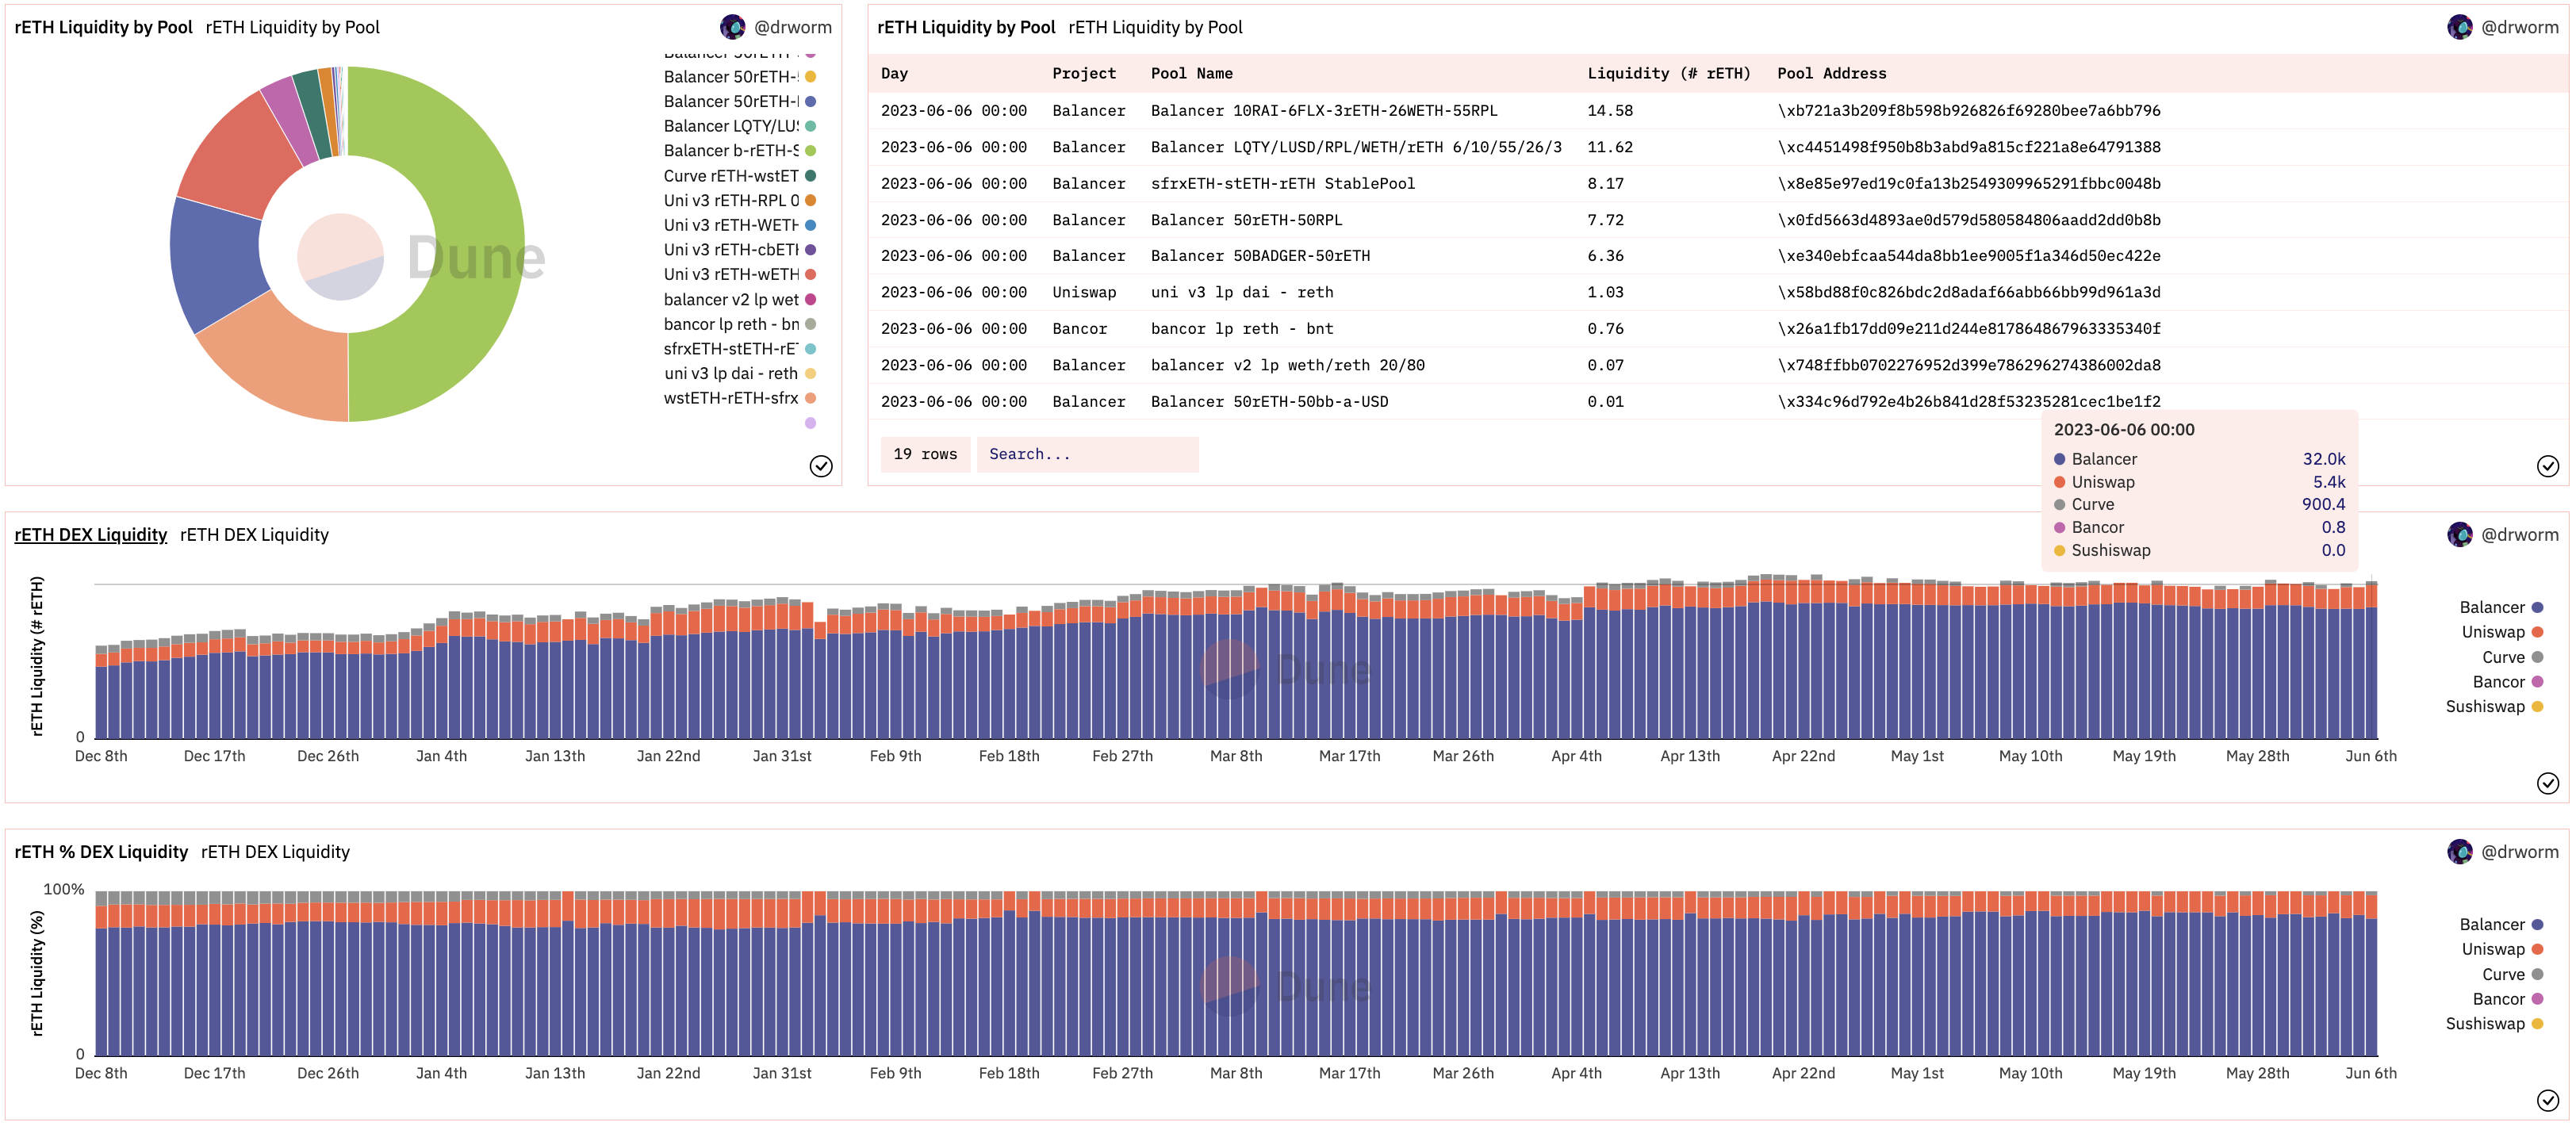
\includegraphics[width=\linewidth]{../images/rocketdrworm5}
%\caption{Dune Analytics Rocket Pool rETH liquidity by @drworm  (7 June 2023)}
%\label{fig:rocketdrworm5}
%\end{center}
%\end{figure}
%
%\begin{figure}[htbp]
%\begin{center}
%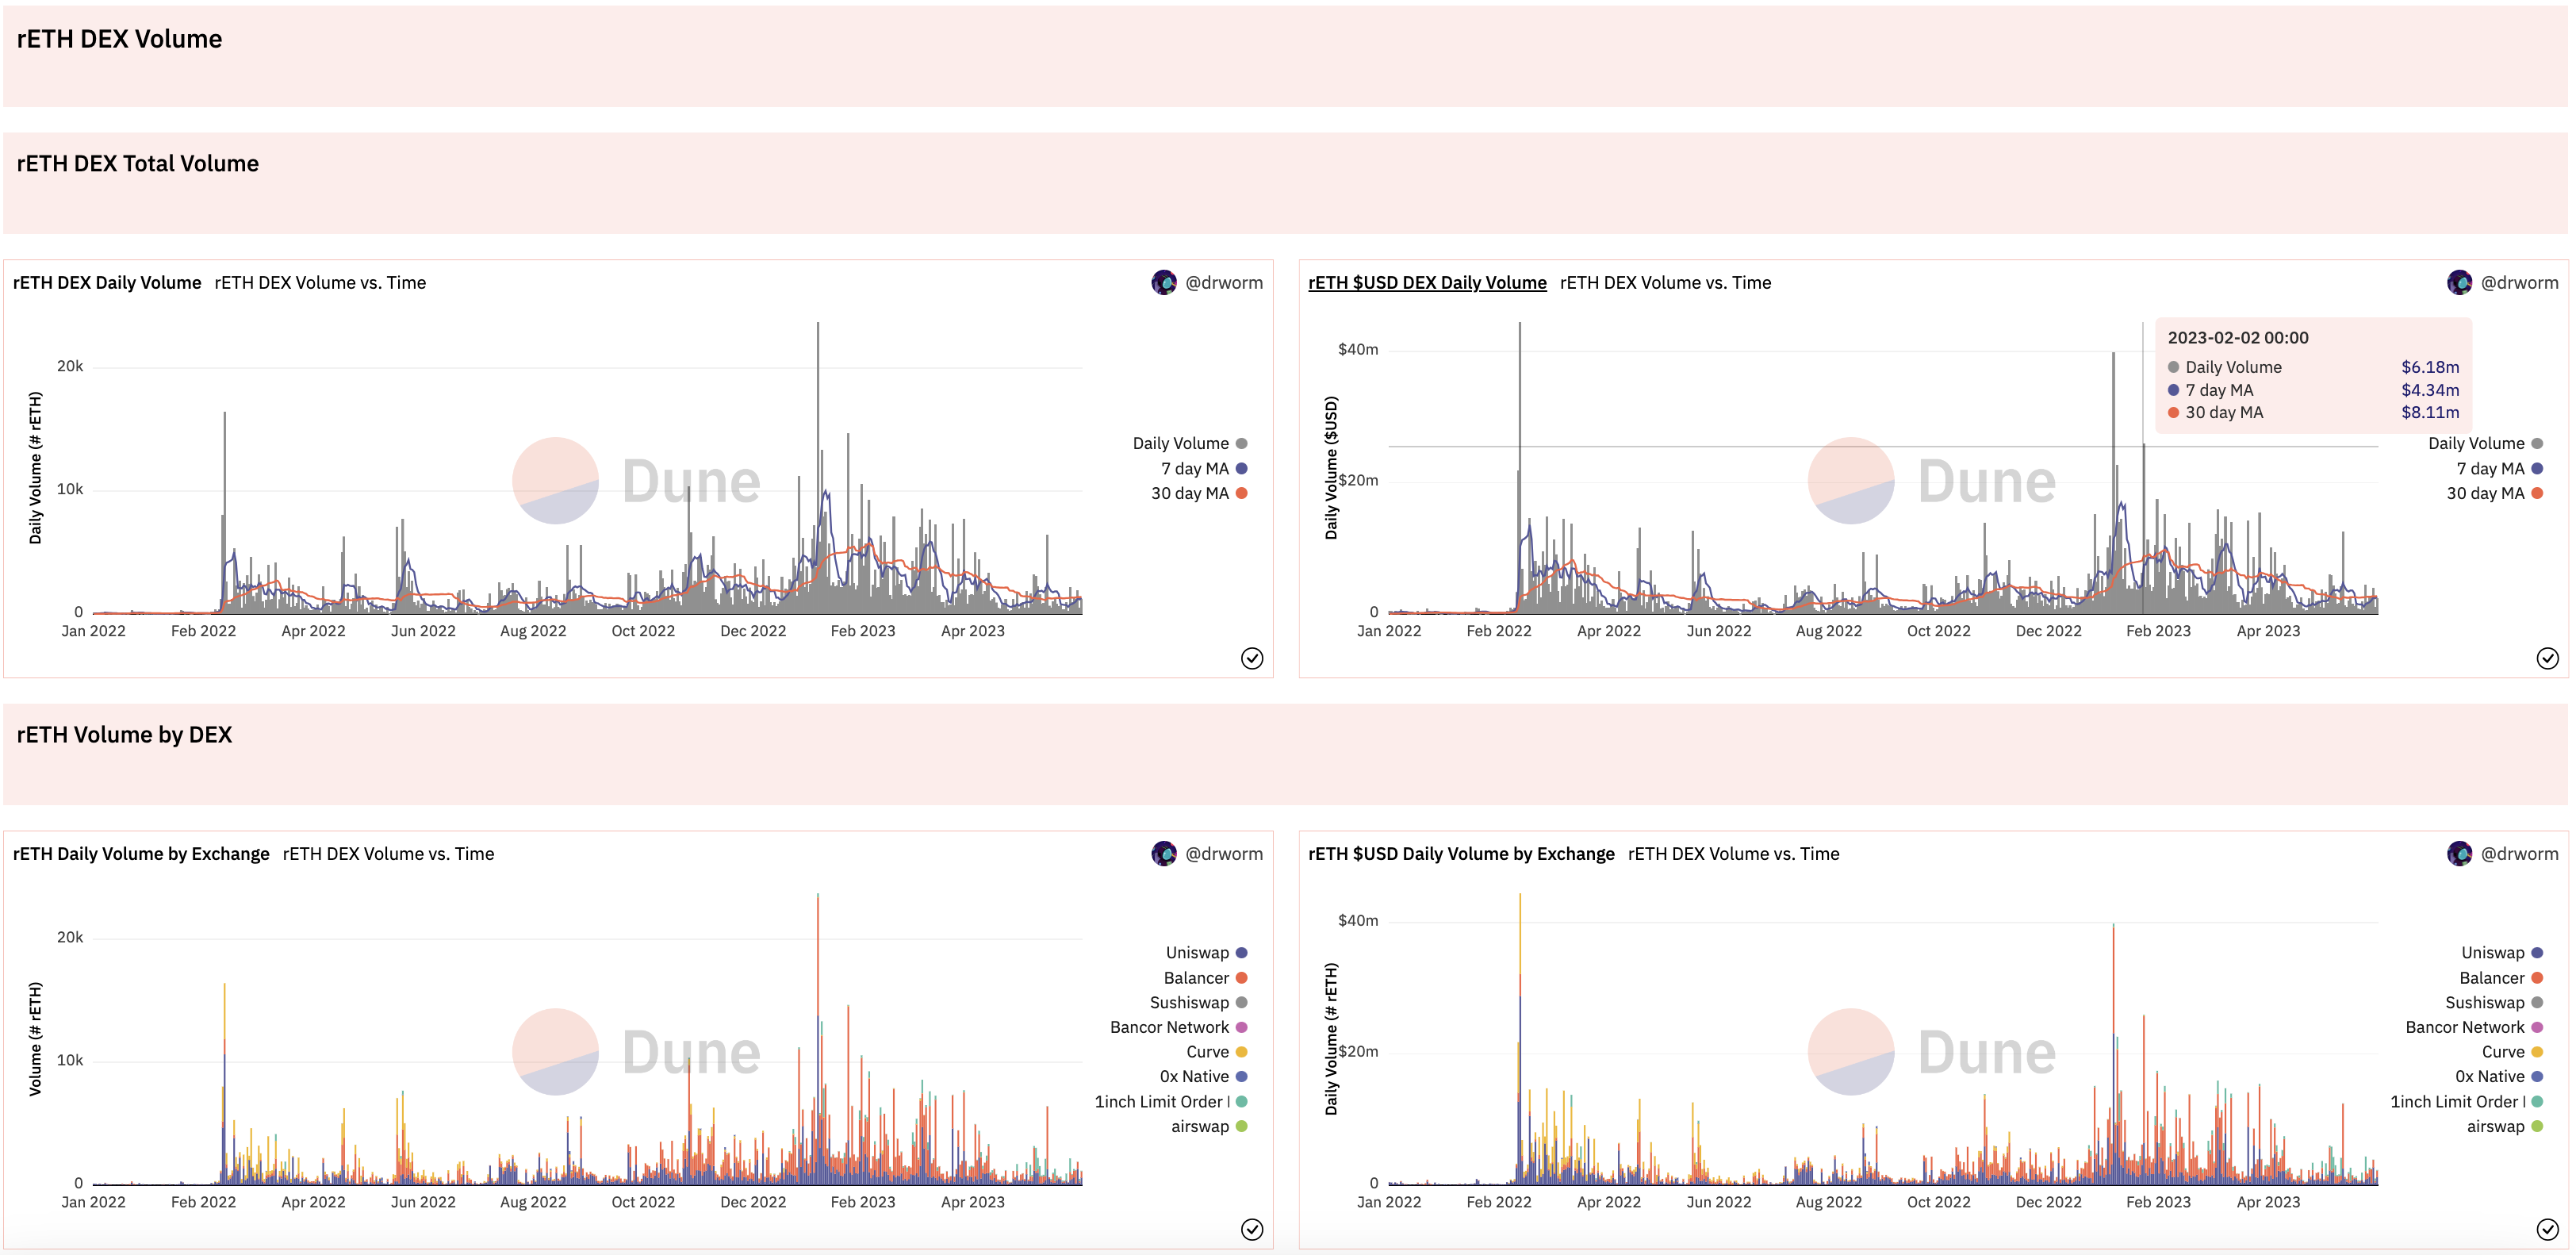
\includegraphics[width=\linewidth]{../images/rocketdrworm6}
%\caption{Dune Analytics Rocket Pool rETH DEX statistics by @drworm  (7 June 2023)}
%\label{fig:rocketdrworm6}
%\end{center}
%\end{figure}
%
%\begin{figure}[htbp]
%\begin{center}
%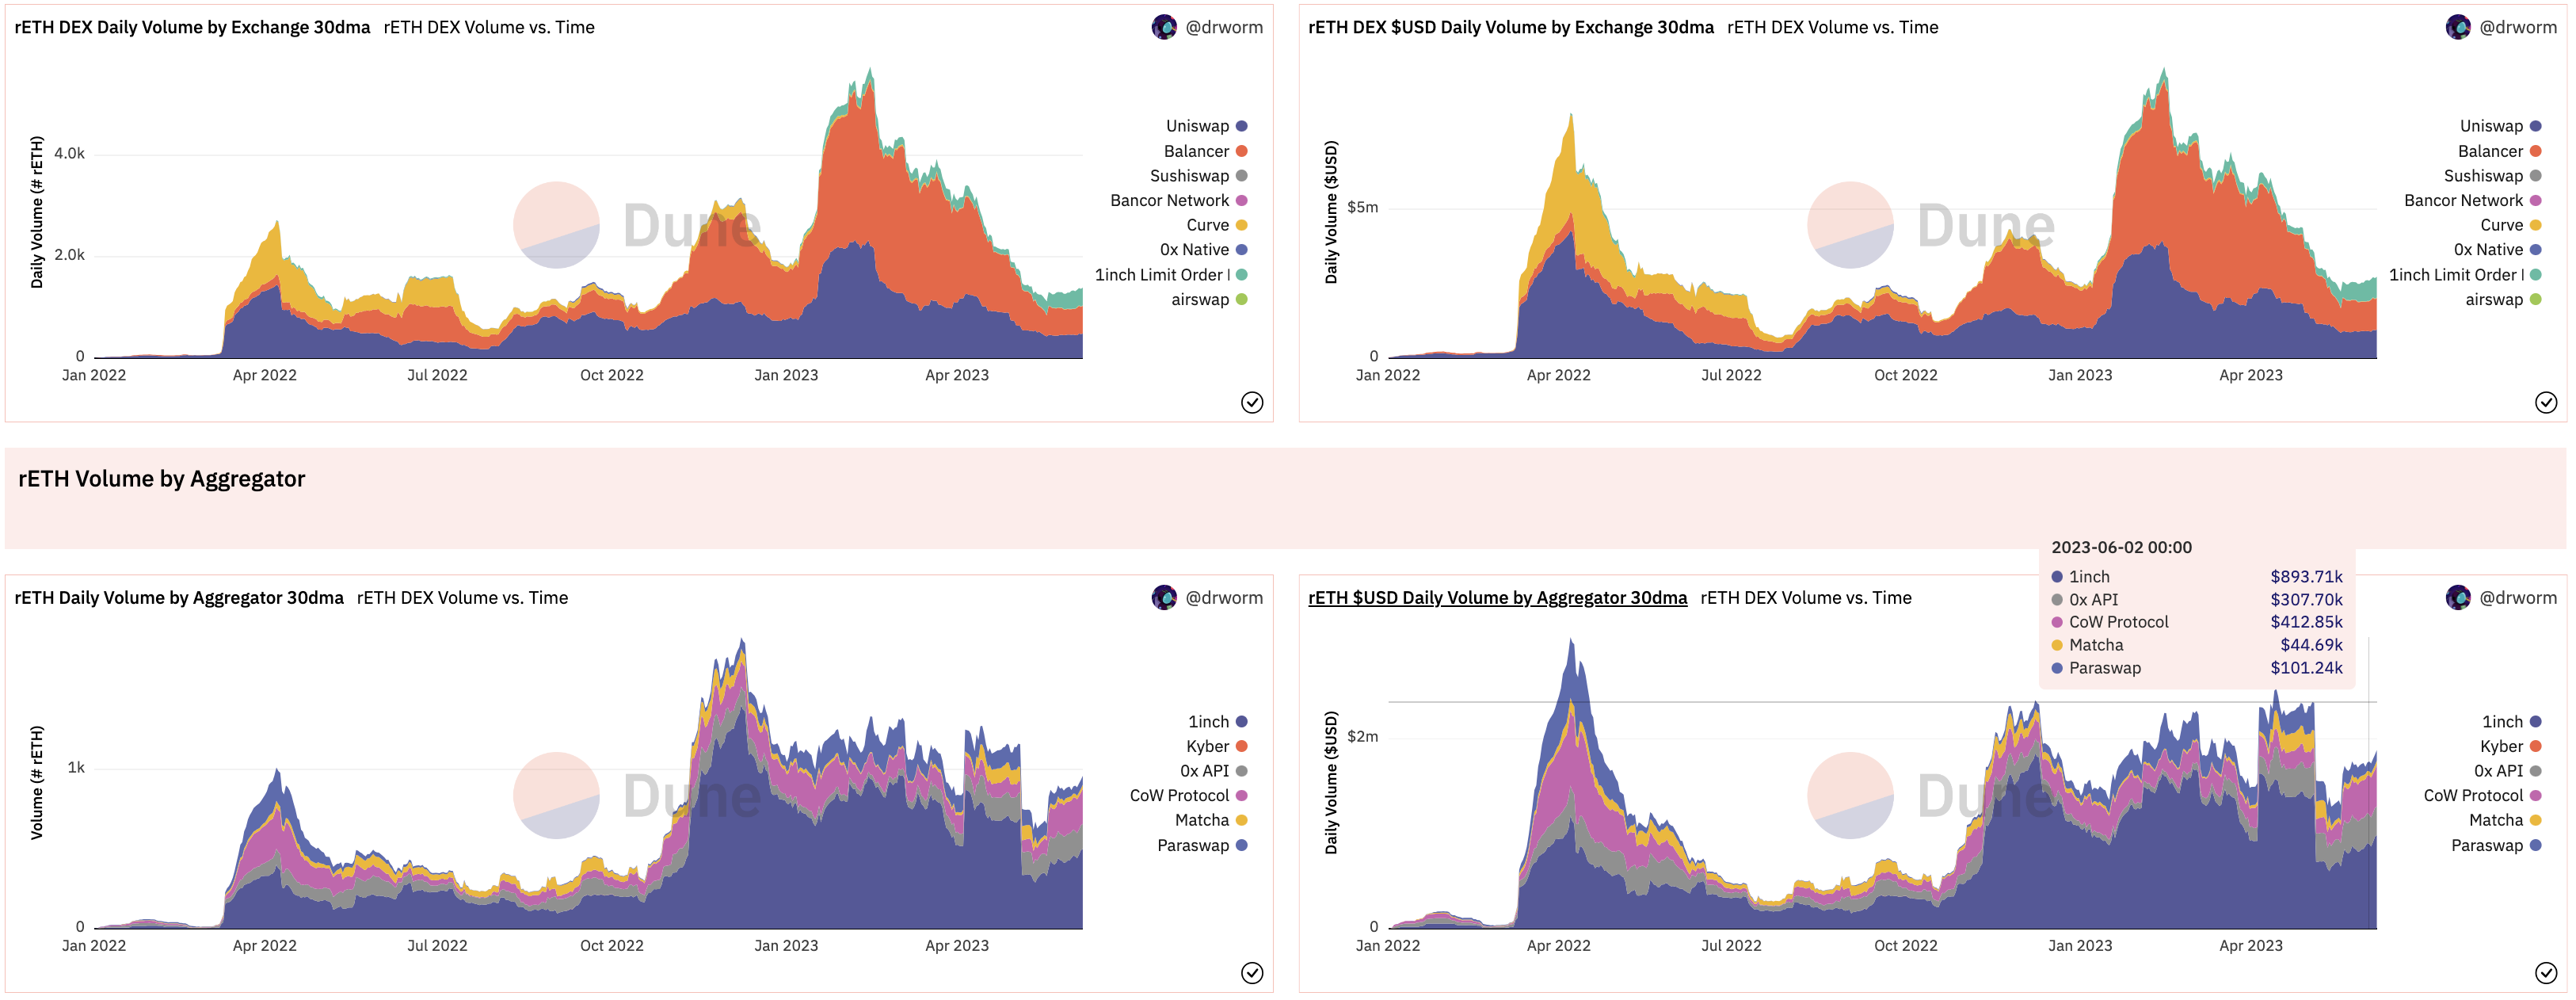
\includegraphics[width=\linewidth]{../images/rocketdrworm7}
%\caption{Dune Analytics Rocket Pool rETH DEX graphs by @drworm  (7 June 2023)}
%\label{fig:rocketdrworm7}
%\end{center}
%\end{figure}
%
%\begin{figure}[htbp]
%\begin{center}
%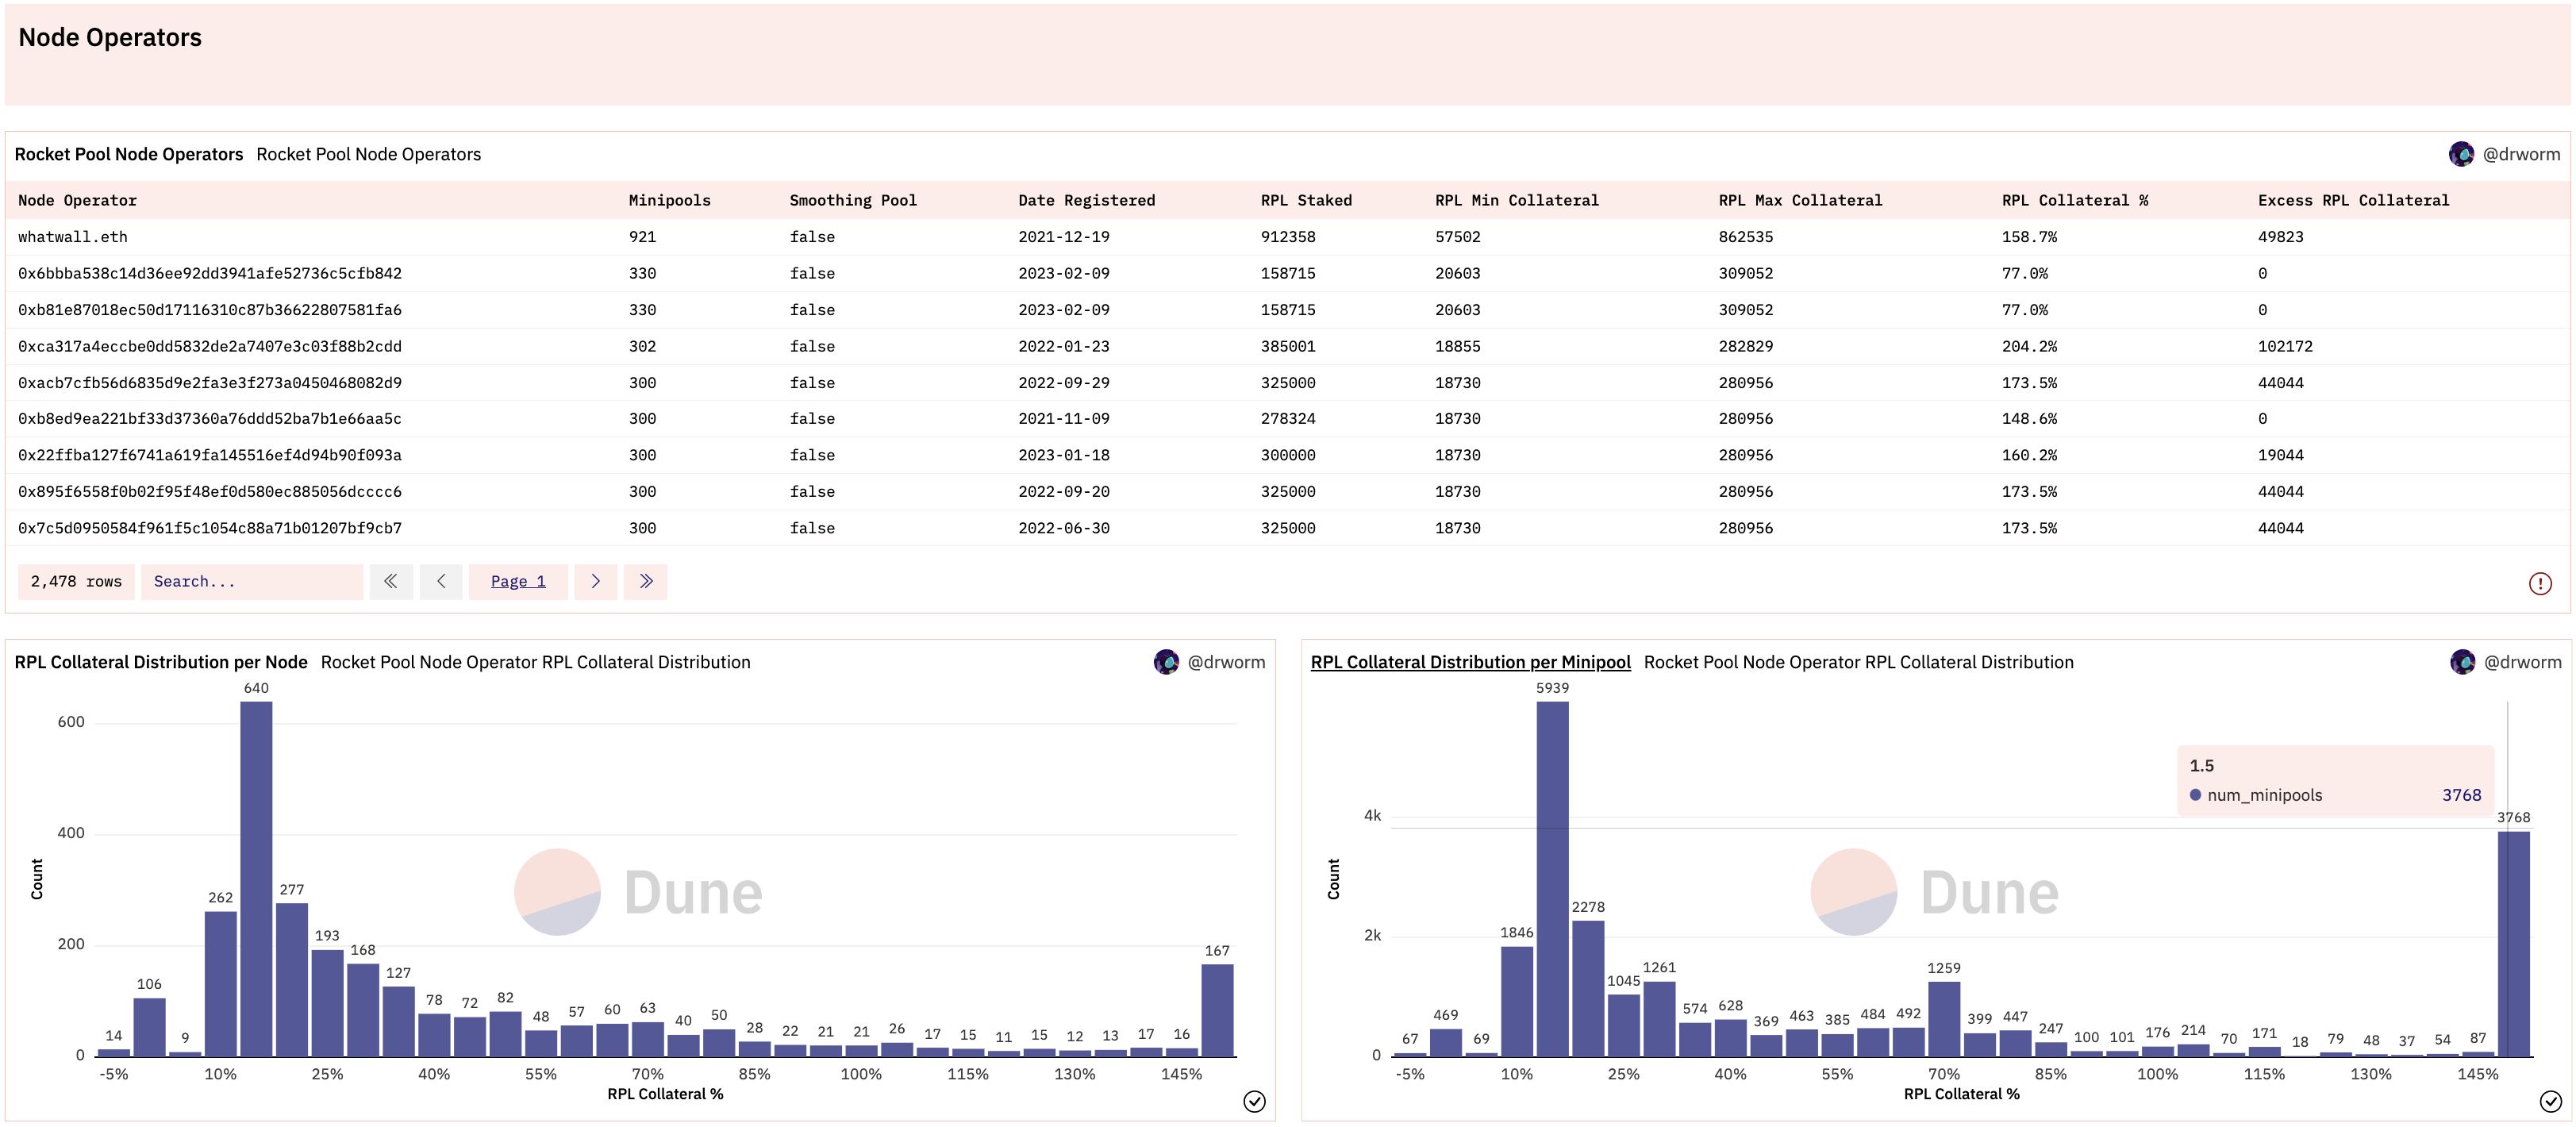
\includegraphics[width=\linewidth]{../images/rocketdrworm8}
%\caption{Dune Analytics Rocket Pool node operators by @drworm  (7 June 2023)}
%\label{fig:rocketdrworm8}
%\end{center}
%\end{figure}
%
%\begin{figure}[htbp]
%\begin{center}
%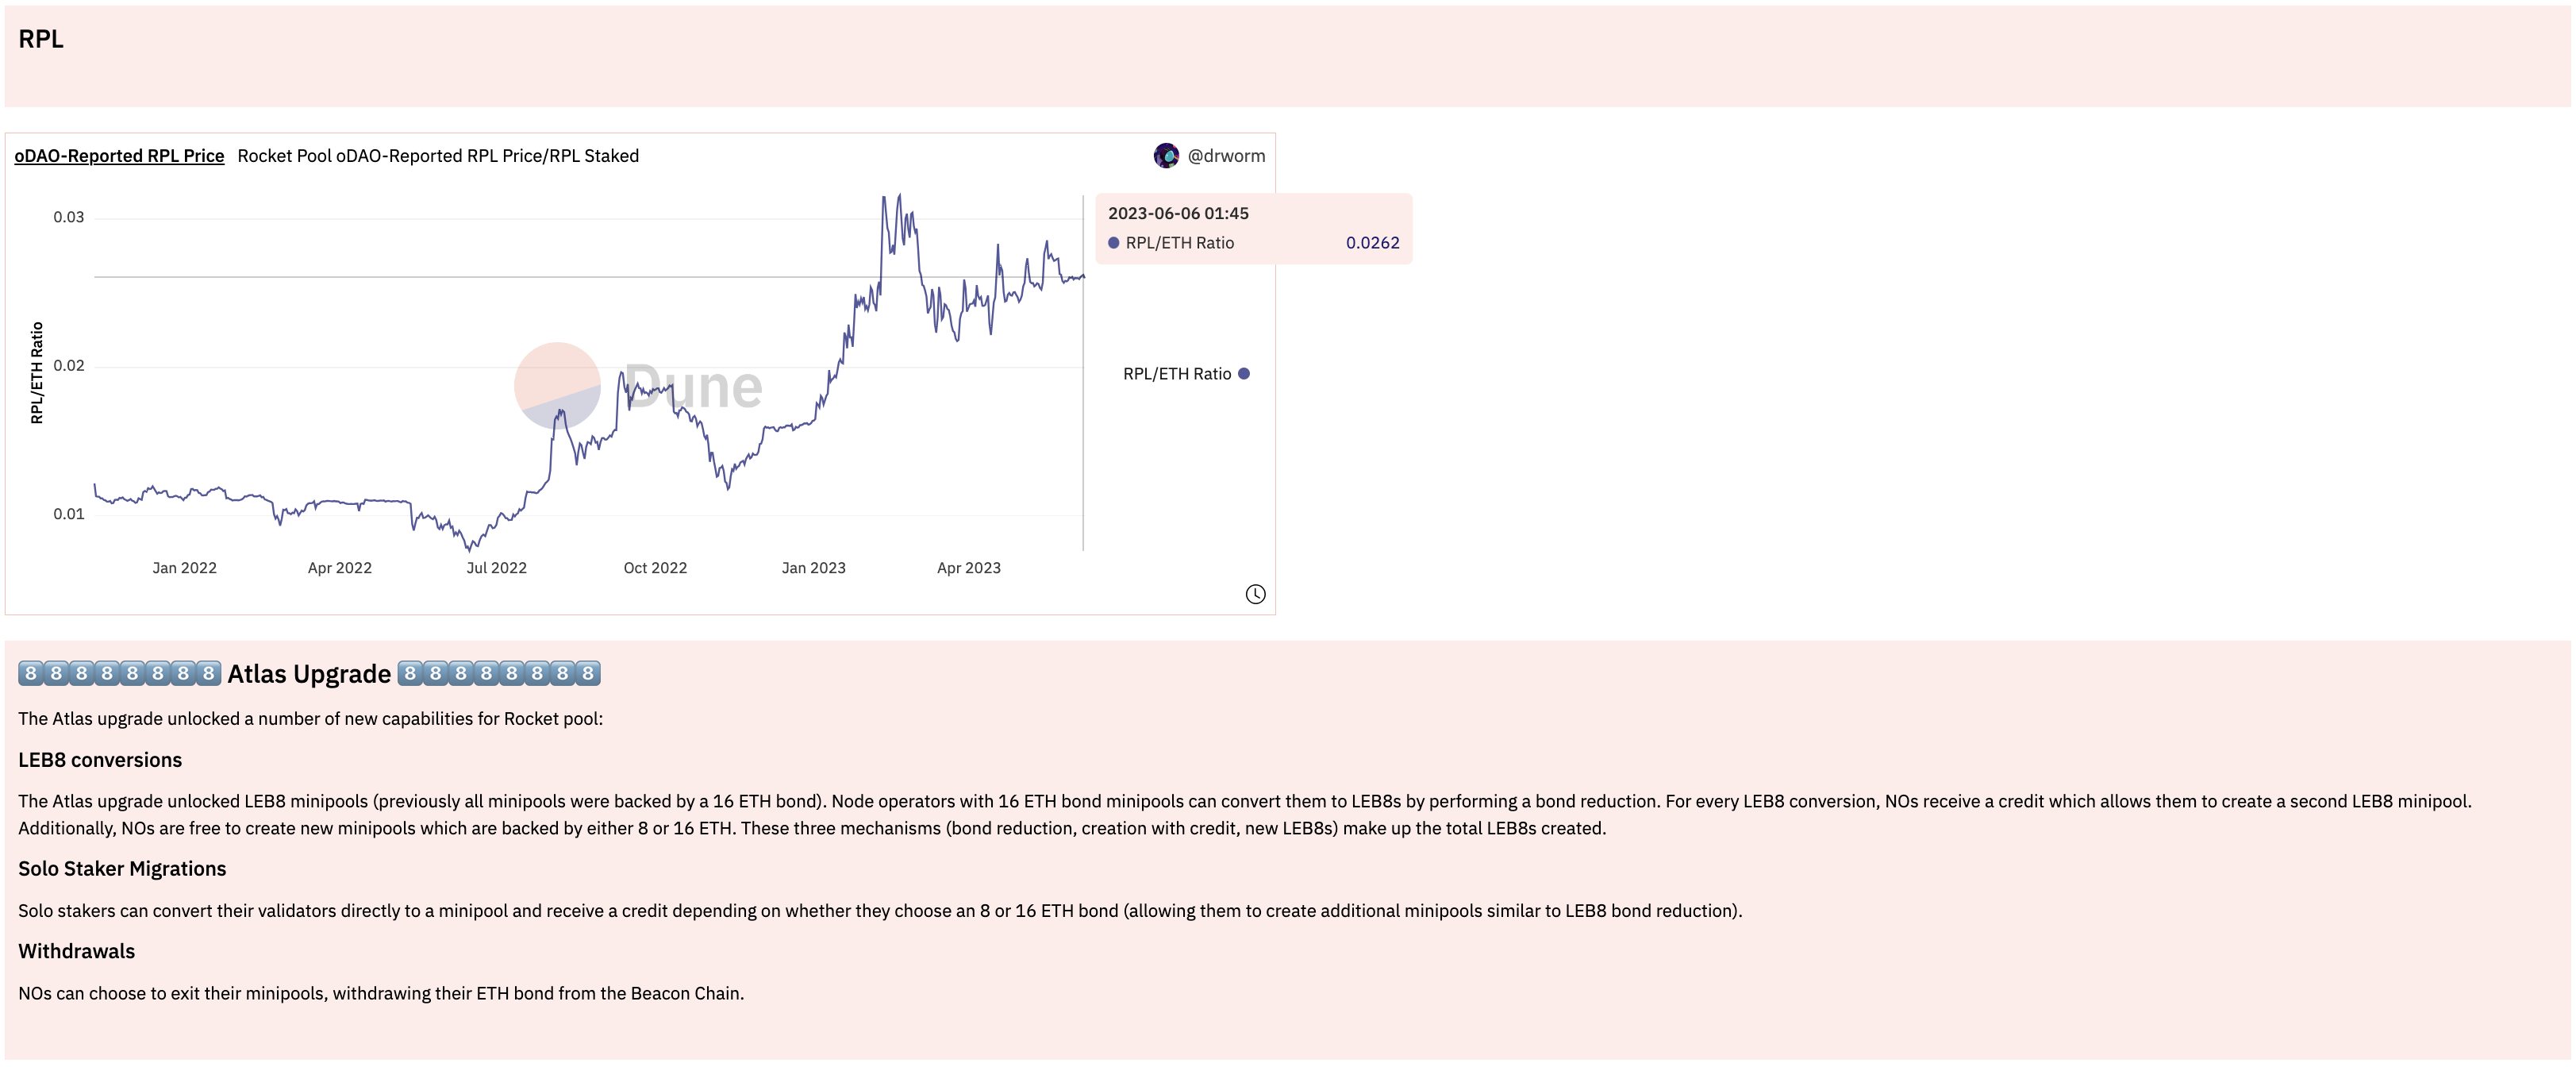
\includegraphics[width=\linewidth]{../images/rocketdrworm9}
%\caption{Dune Analytics Rocket Pool oDAO-Reported RPL Price/RPL Staked by @drworm  (7 June 2023)}
%\label{fig:rocketdrworm9}
%\end{center}
%\end{figure}
%
%\begin{figure}[htbp]
%\begin{center}
%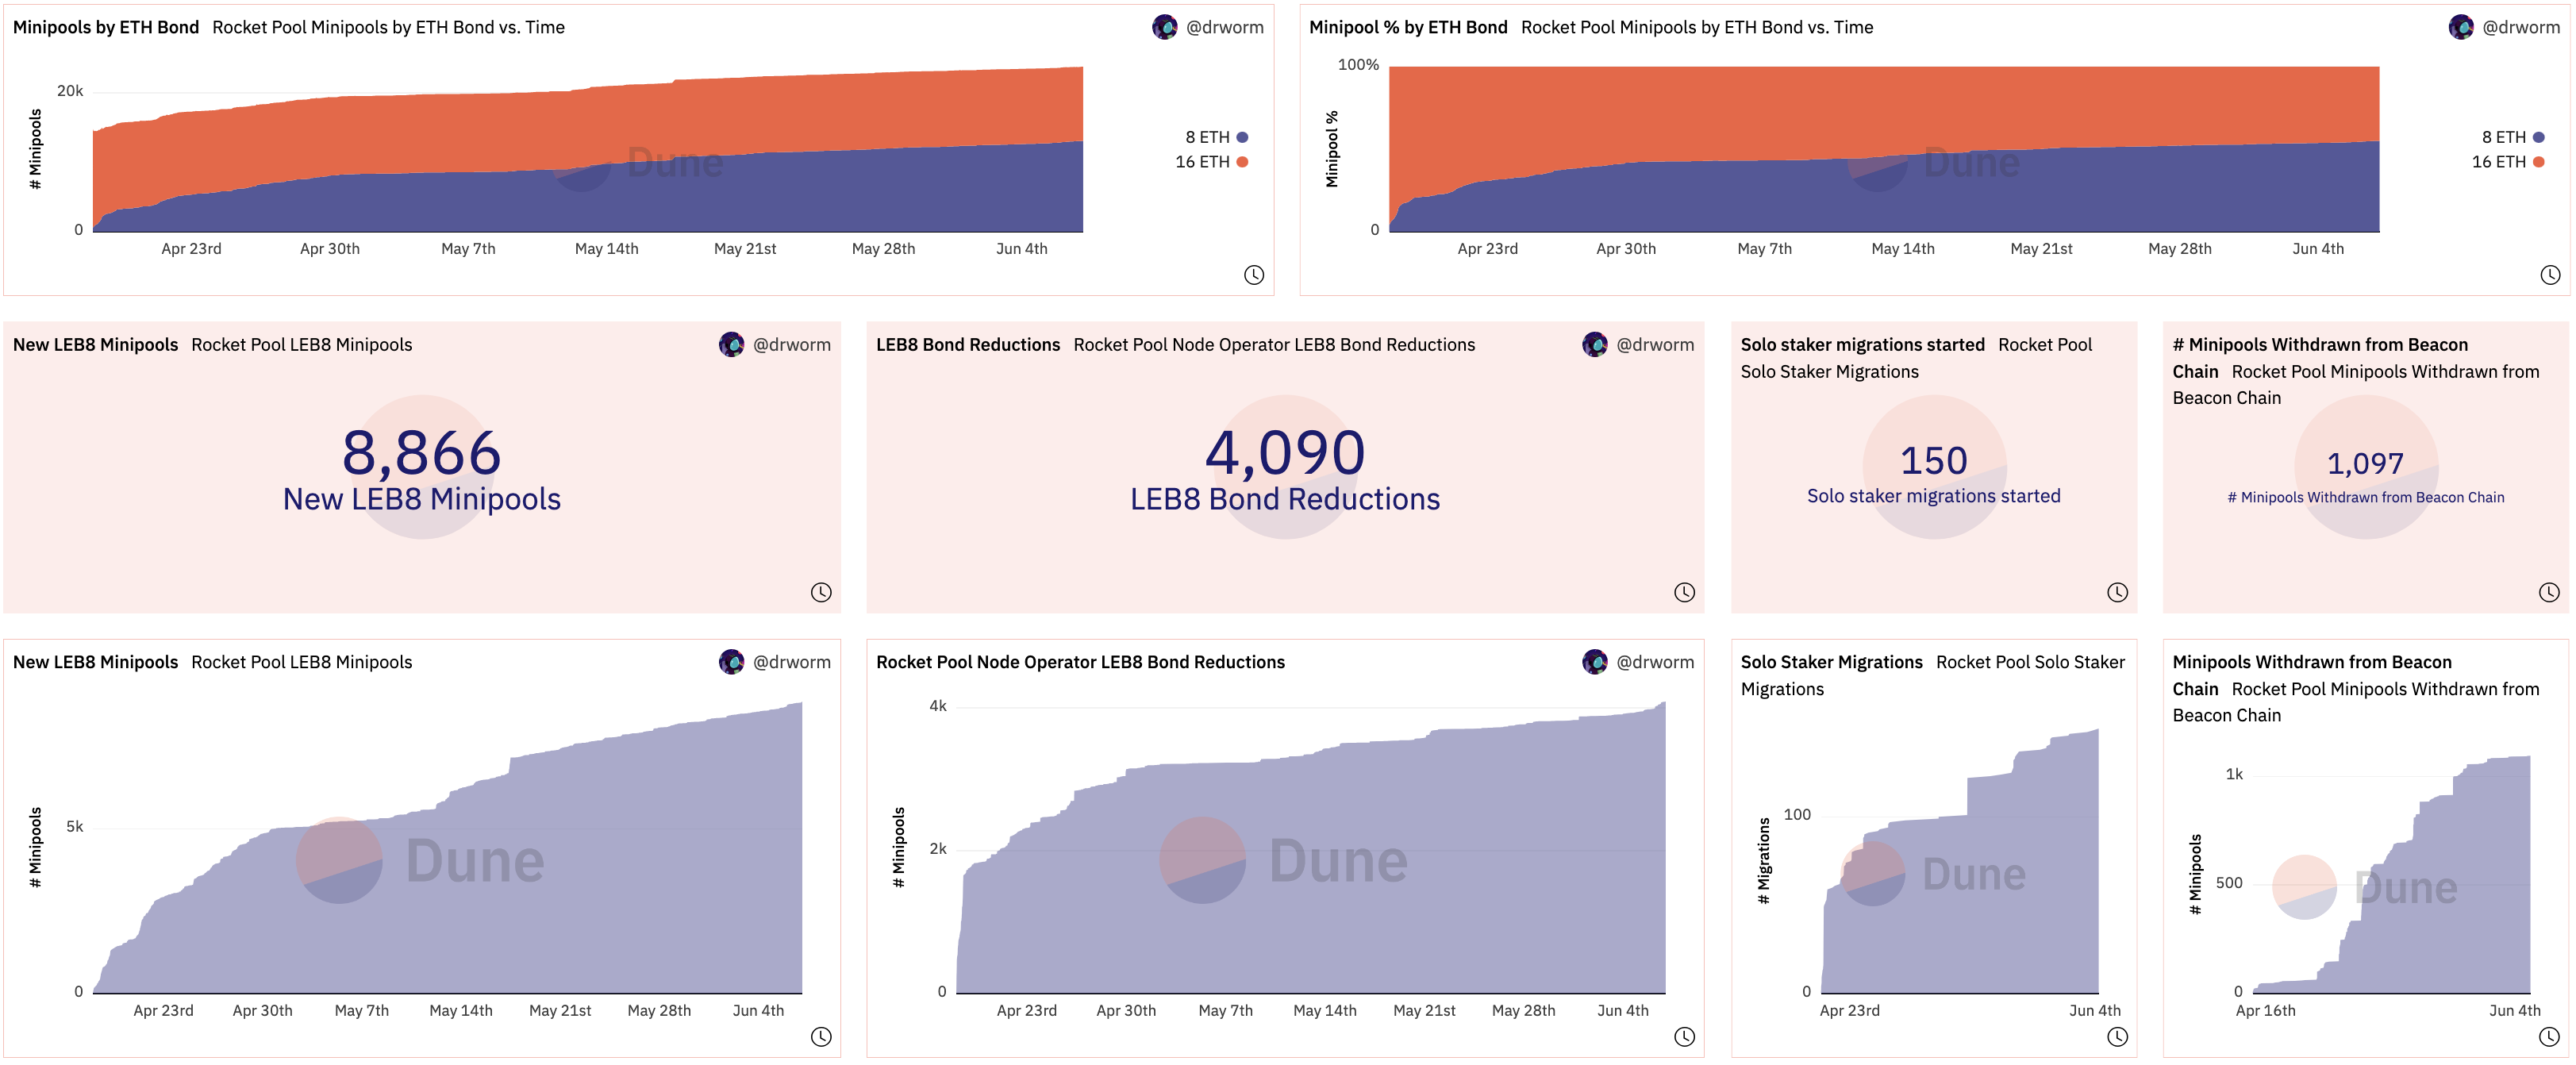
\includegraphics[width=\linewidth]{../images/rocketdrworm10}\\
%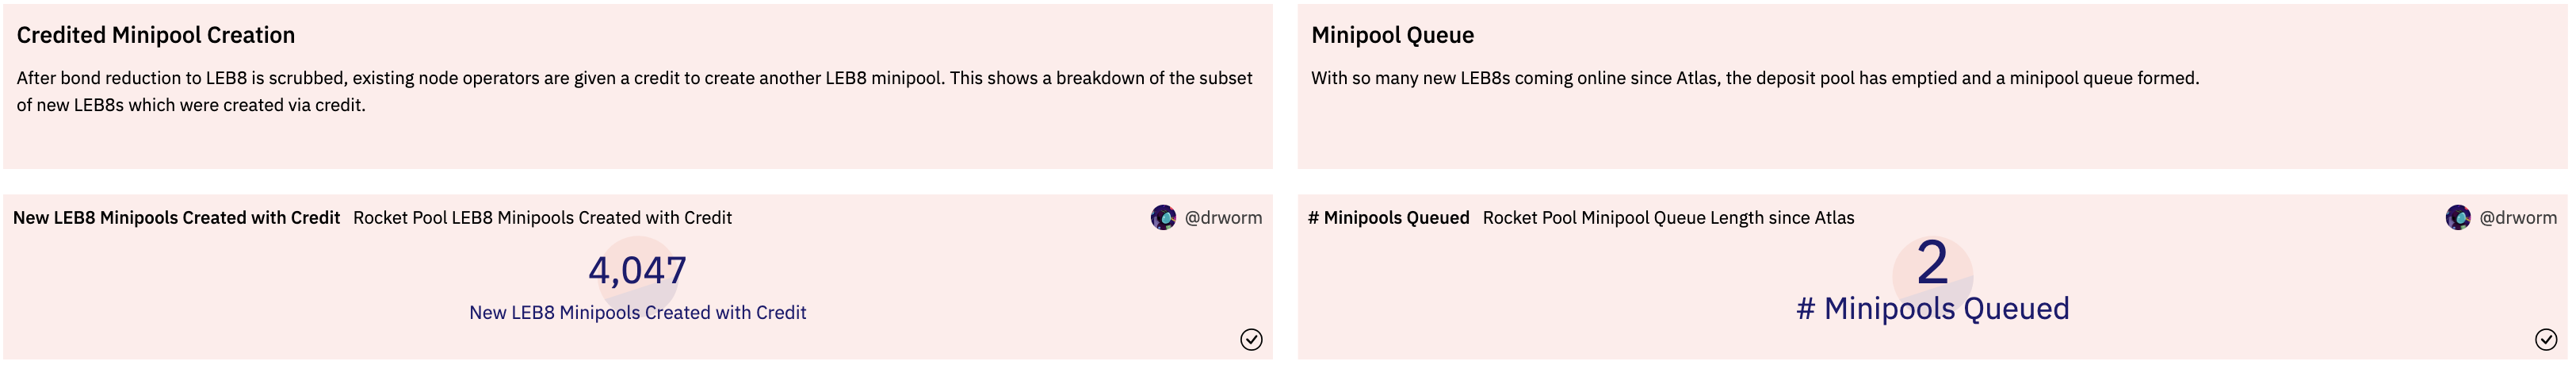
\includegraphics[width=\linewidth]{../images/rocketdrworm11}
%\caption{Dune Analytics Rocket Pool Minipools by @drworm  (7 June 2023)}
%\label{fig:rocketdrworm10}
%\end{center}
%\end{figure}
%
%\begin{figure}[htbp]
%\begin{center}
%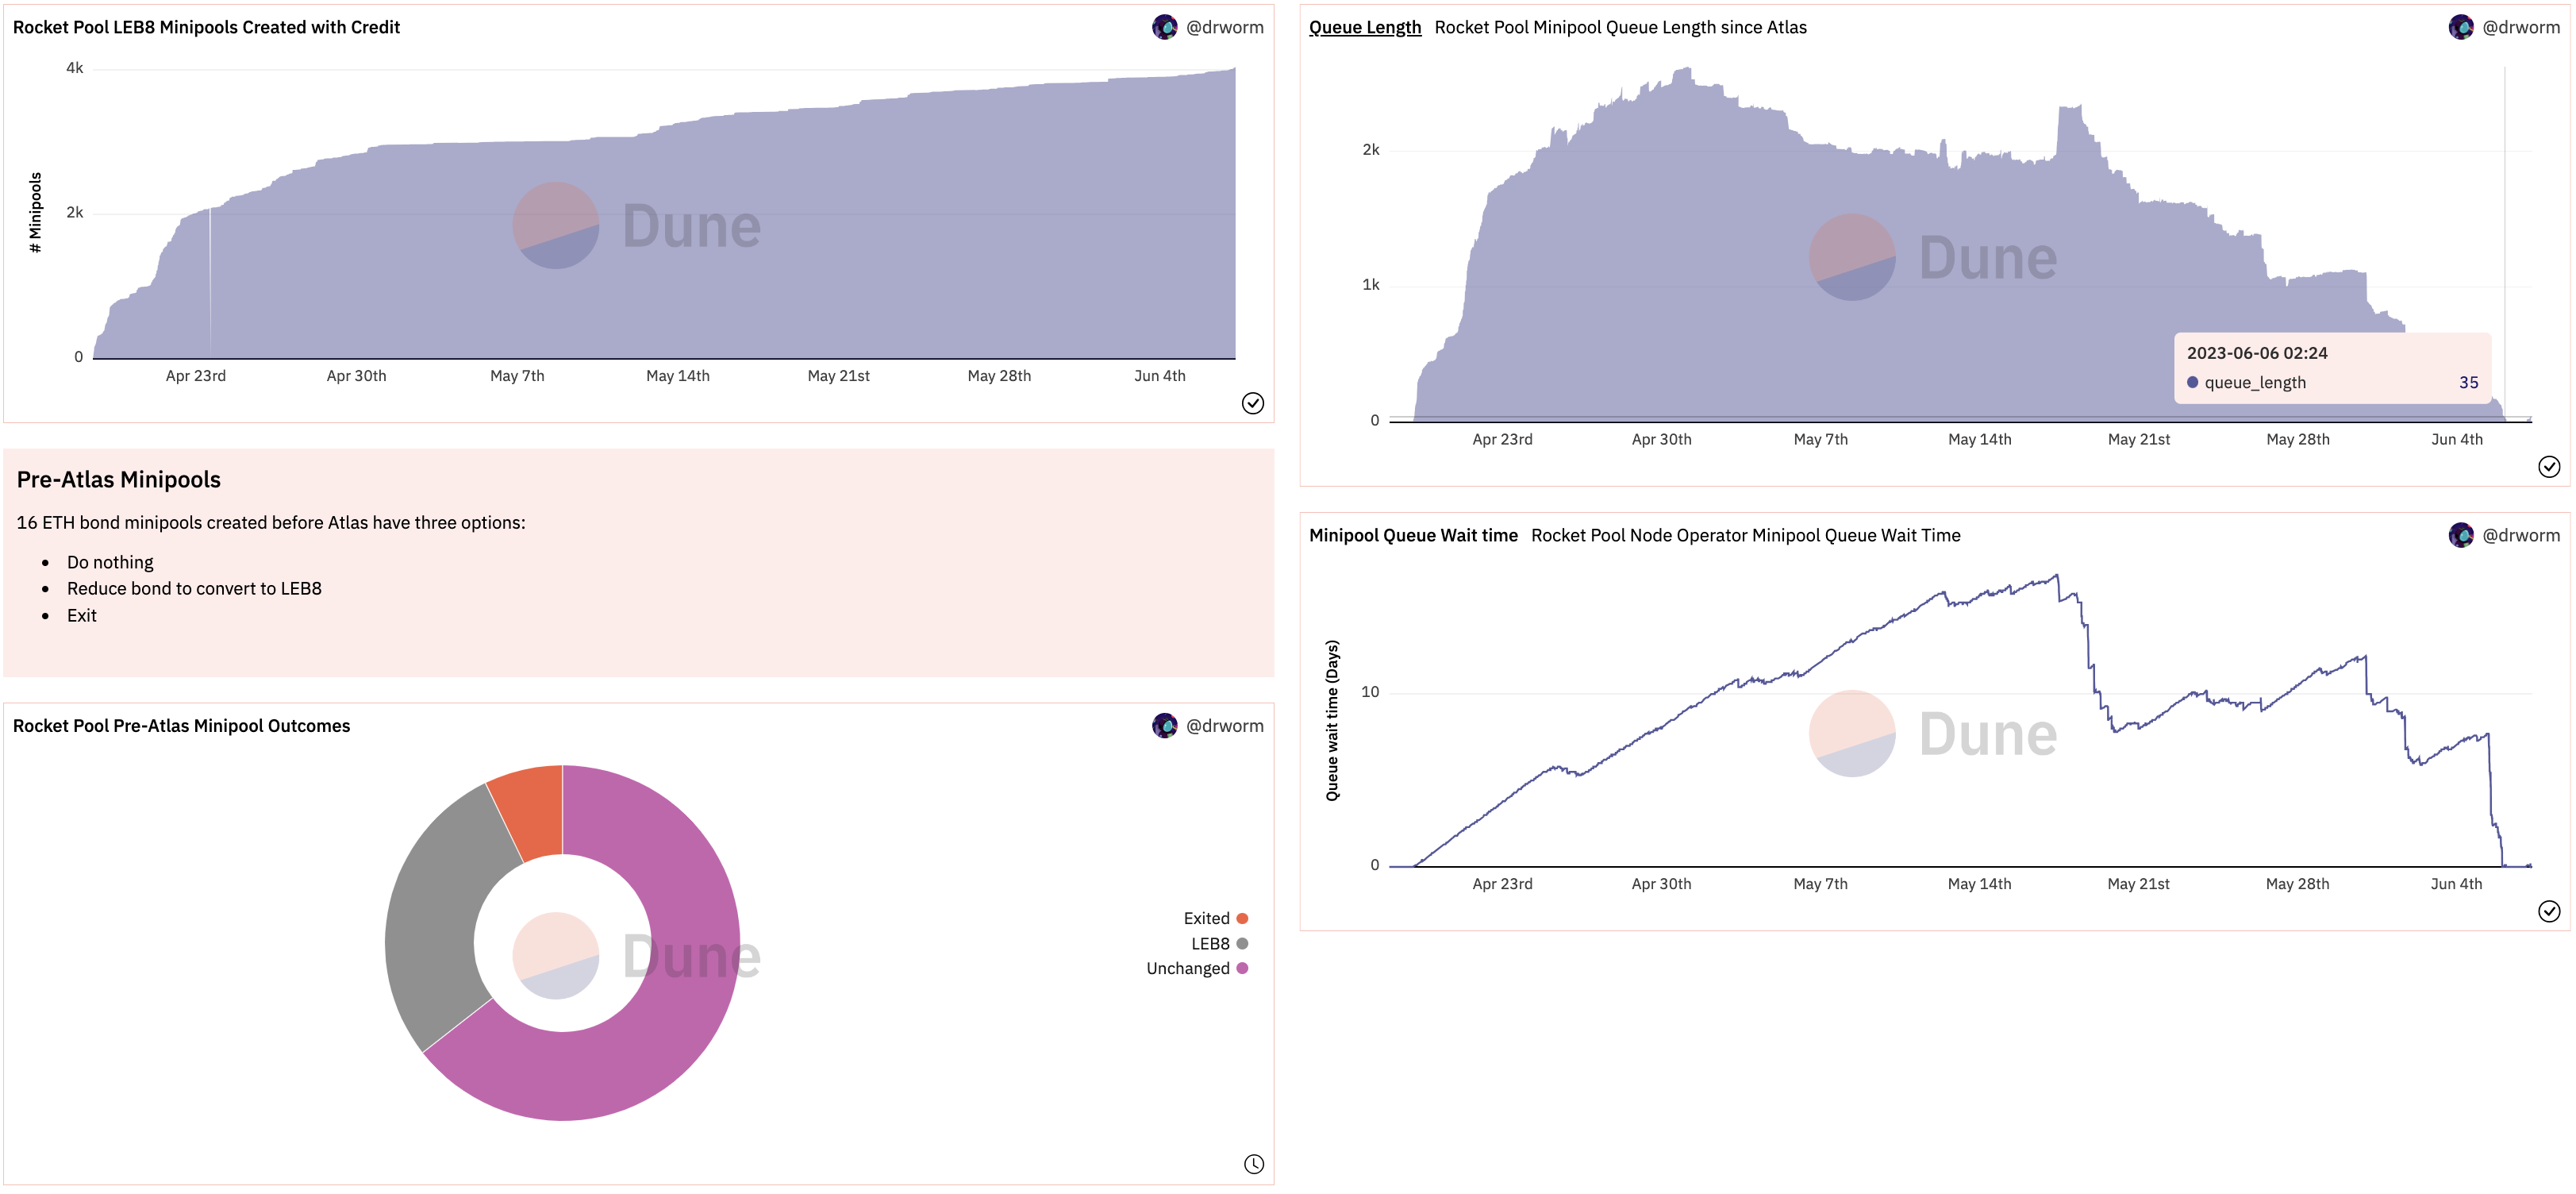
\includegraphics[width=\linewidth]{../images/rocketdrworm12}
%\caption{Dune Analytics Rocket Pool Rocket Pool Minipools by @drworm  (7 June 2023)}
%\label{fig:rocketdrworm12}
%\end{center}
%\end{figure}
%
%\clearpage

% ---------------------------------------------------------------
\subsection{Staker wealth and distribution}
% ---------------------------------------------------------------
%
%\begin{figure}[htbp]
%\begin{center}
%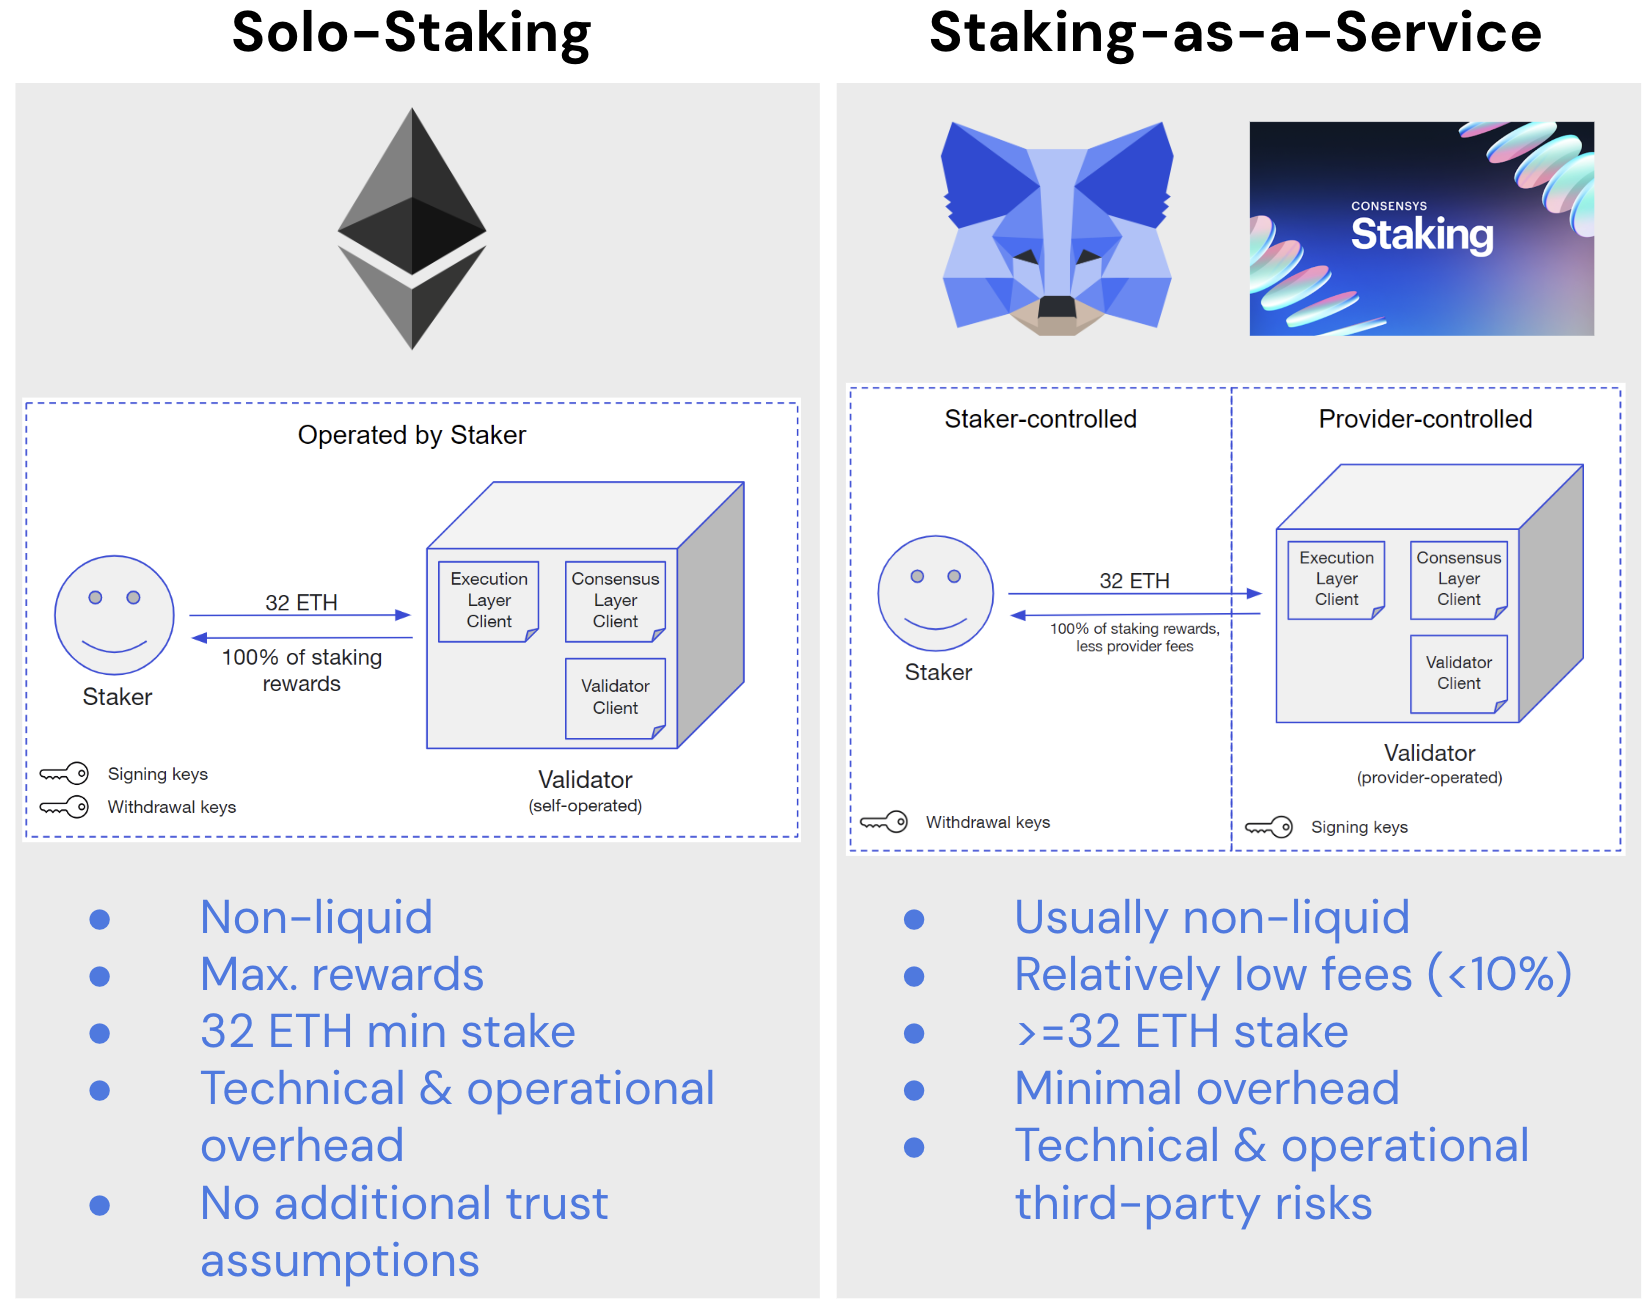
\includegraphics[width=0.7\linewidth]{../images/solo-saas}
%\caption{Solo staking, staking as a service (credit: Andrew Breslin)}
%\label{fig:solo}
%\end{center}
%\end{figure}
%
%\begin{figure}[htbp]
%\begin{center}
%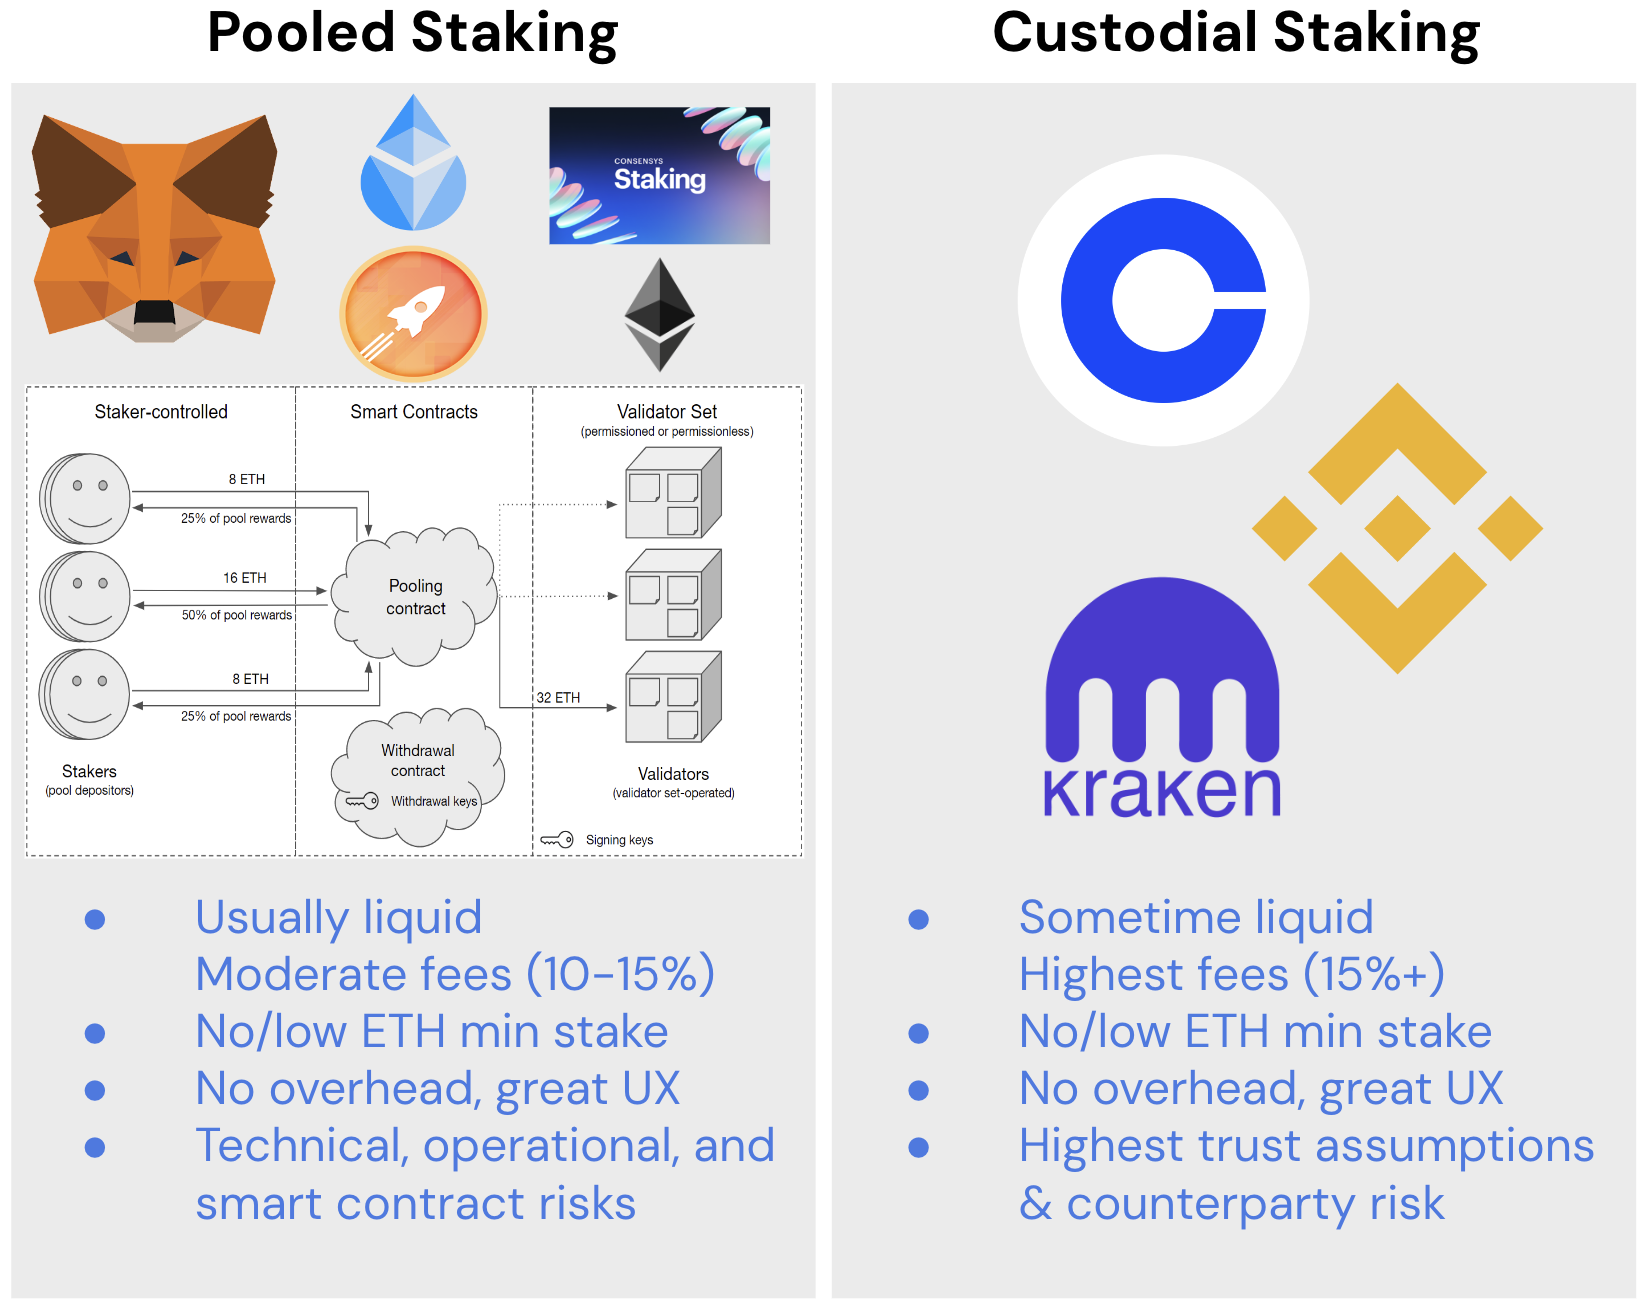
\includegraphics[width=0.7\linewidth]{../images/pooled-custodial}
%\caption{Pooled staking, Custodial staking (credit:Andrew Breslin)}
%\label{fig:pooled}
%\end{center}
%\end{figure}

We can at best have an informed guess about current staker wealth distribution.
Some staking pools can be identified, but even then we may not be aware of all
of the validator nodes and validators that they run. However, the largest
staking pool, Lido, is transparent regarding its overall control of validators.
Lido operates on a trusted setup, and Consensys staking runs several Lido
operators. 
%
%\clearpage
%% --------------------------------------
%\subsubsection*{Rated network explorer}
%% --------------------------------------
%\textbf{Entity Views} \\
%% ----------------------------------
%\begin{figure}[htbp]
%\begin{center}
%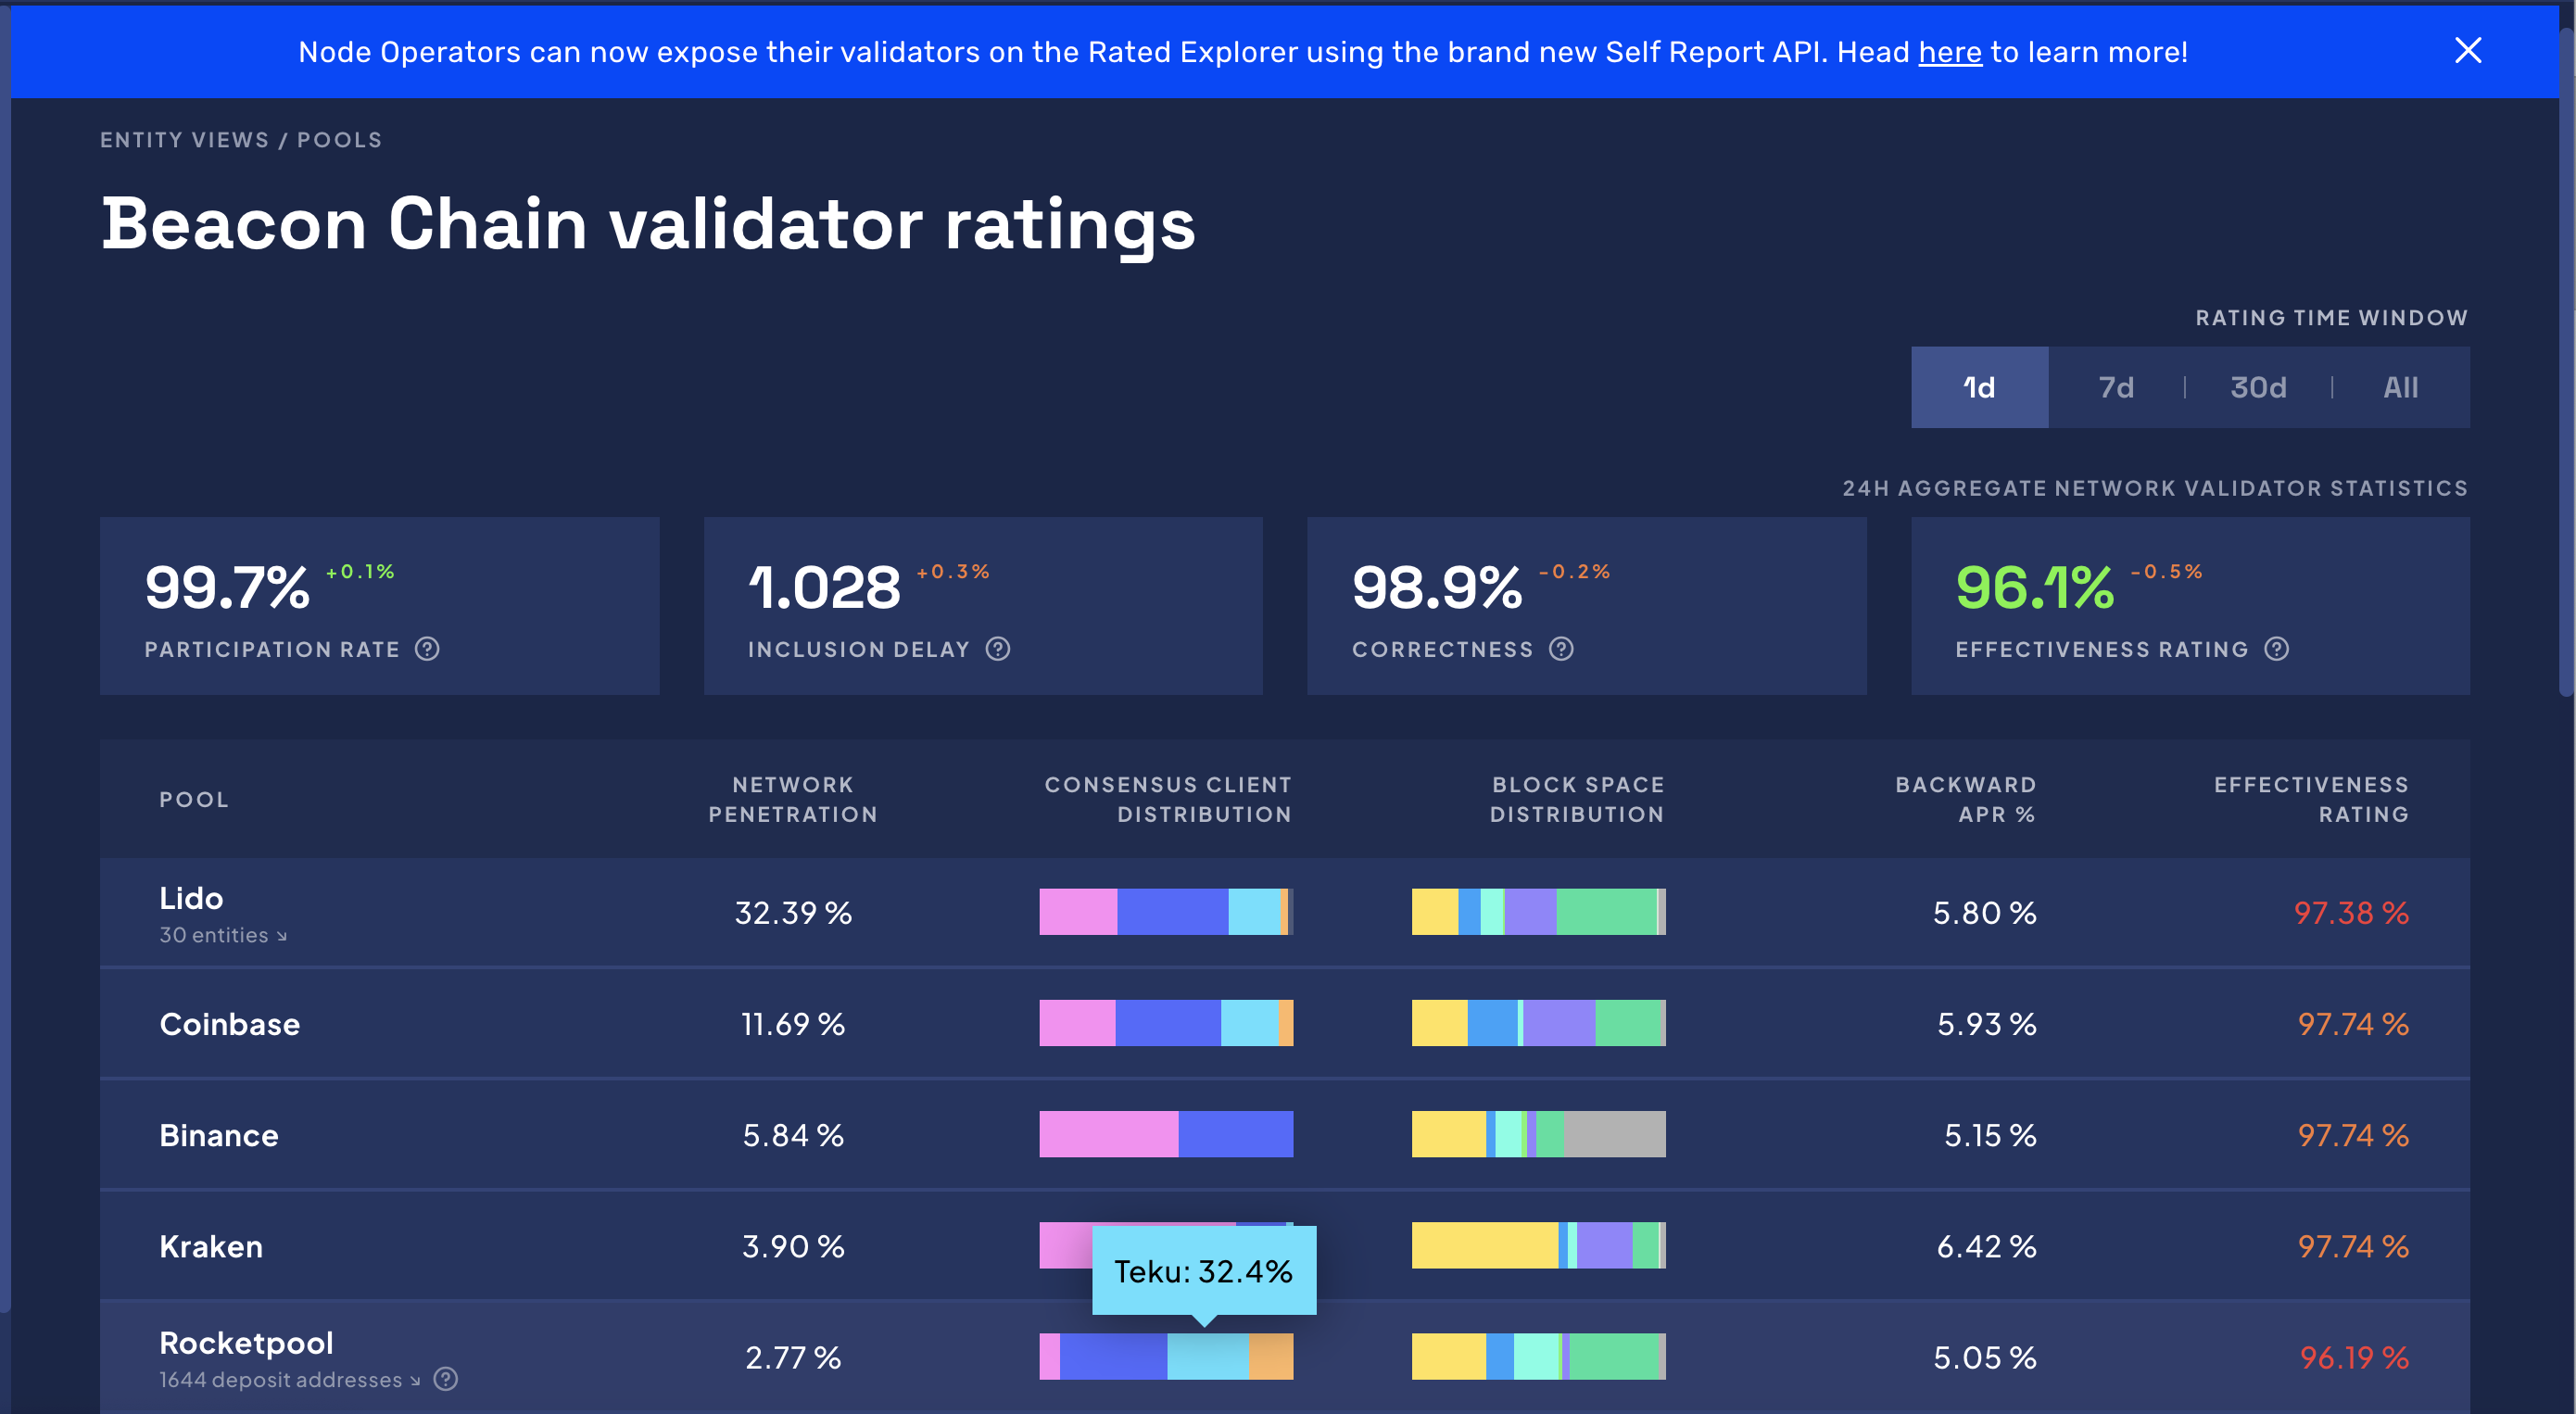
\includegraphics[width=\linewidth]{../images/ratedentity1}
%\caption{Rated network explorer: beacon chain validator ratings for staking pools. Select from timeframes: 1 day, 7 days, 30 days, or all (since merge) , 1 June 2023}
%\label{fig:ratedentity1}
%\end{center}
%\end{figure}
%
%\begin{figure}[htbp]
%\begin{center}
%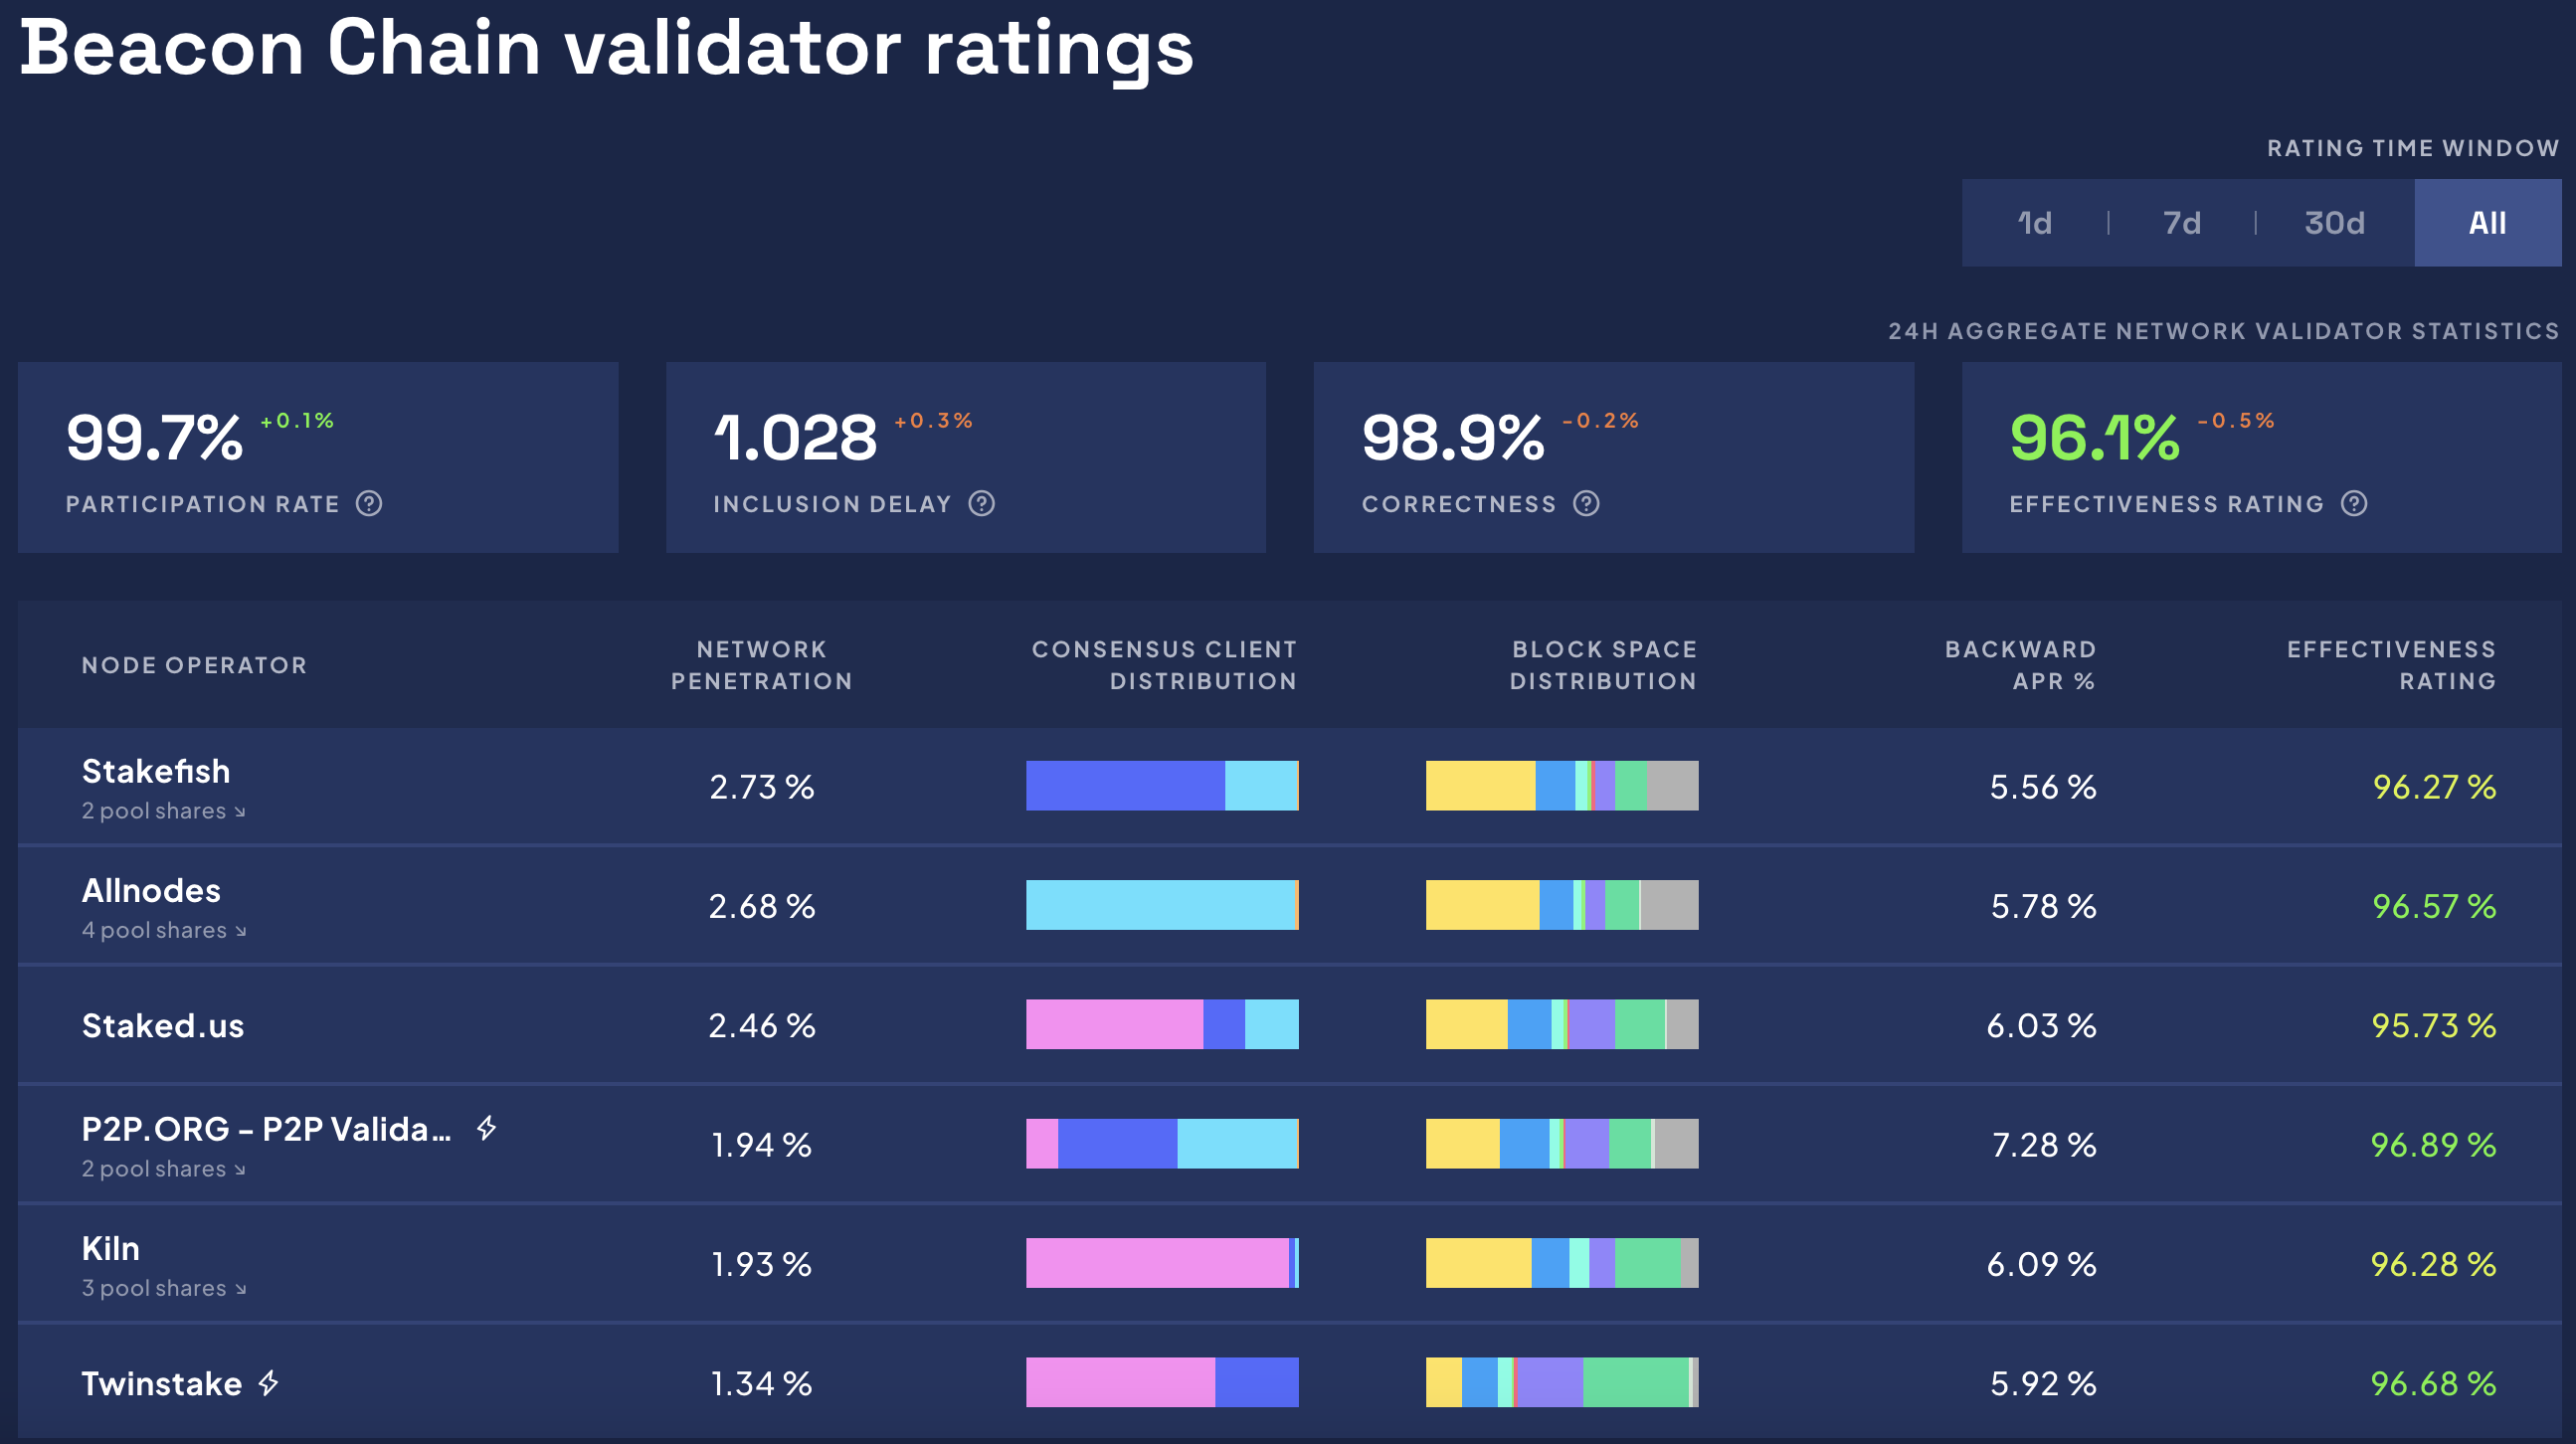
\includegraphics[width=\linewidth]{../images/ratedentity2}
%\caption{Rated network explorer: beacon chain validator ratings for node operators. Select from timeframes: 1 day, 7 days, 30 days, or all (since merge) , 1 June 2023}
%\label{fig:ratedentity2}
%\end{center}
%\end{figure}
%
%\noindent
%\textbf{Aggregate Views} 
%% ----------------------------------
%\begin{figure}[htbp]
%\begin{center}
%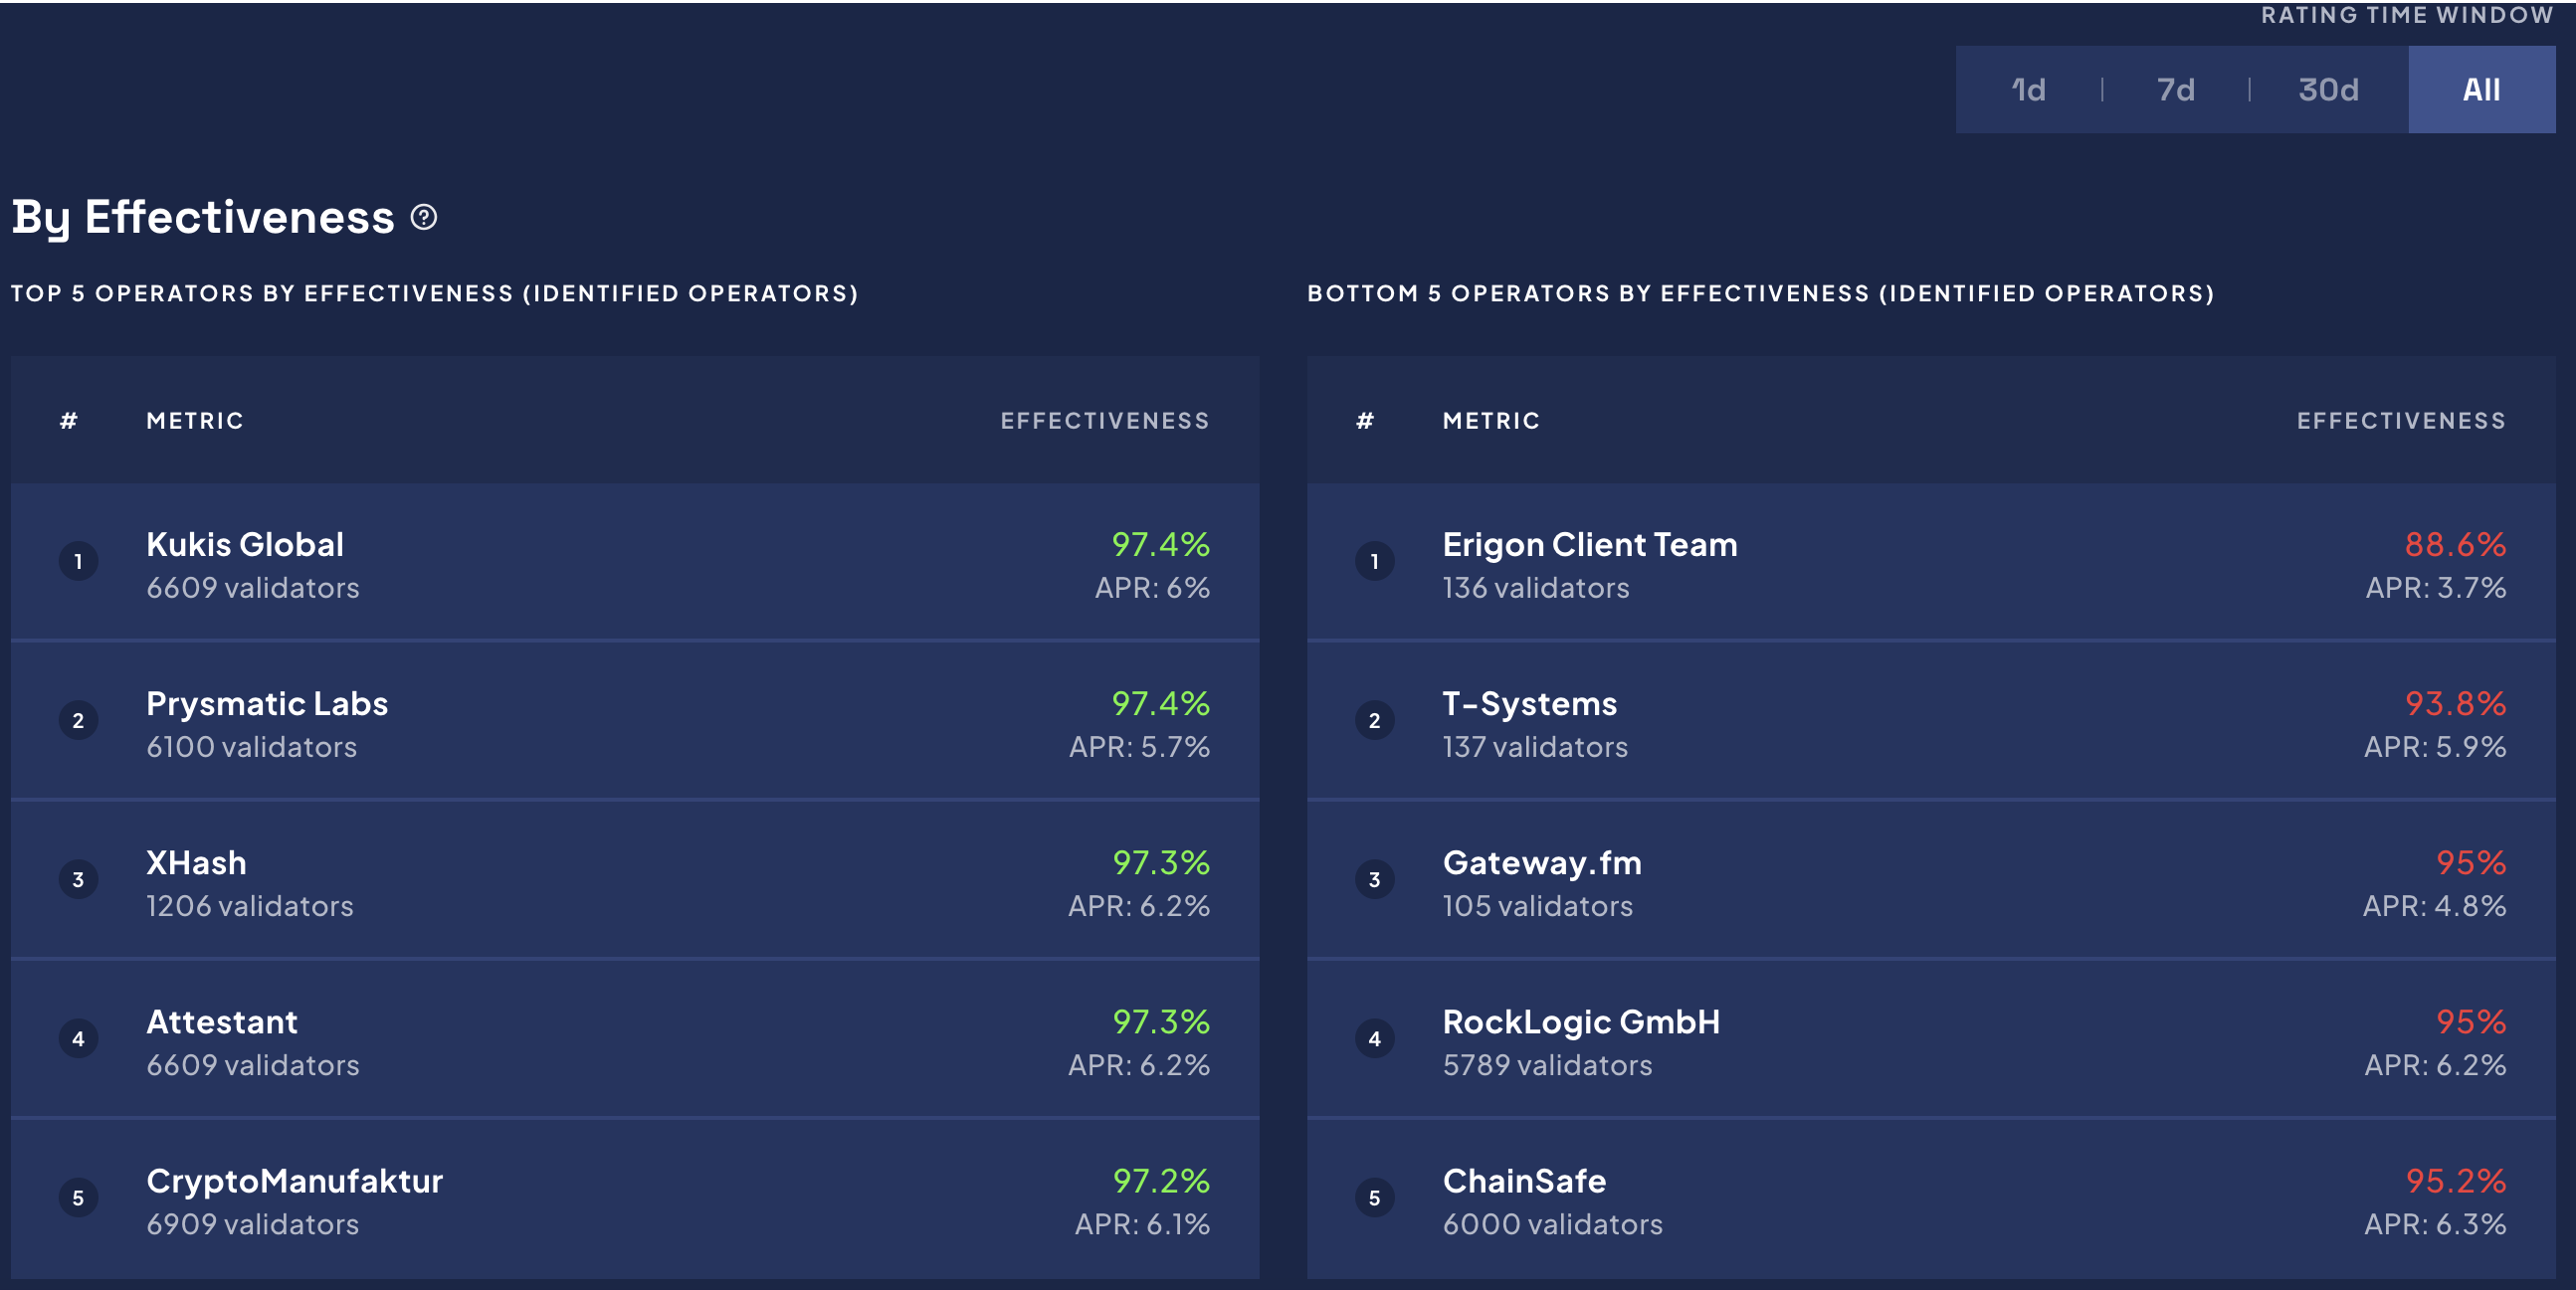
\includegraphics[width=\linewidth]{../images/ratedtrend1}\\
%(a)
%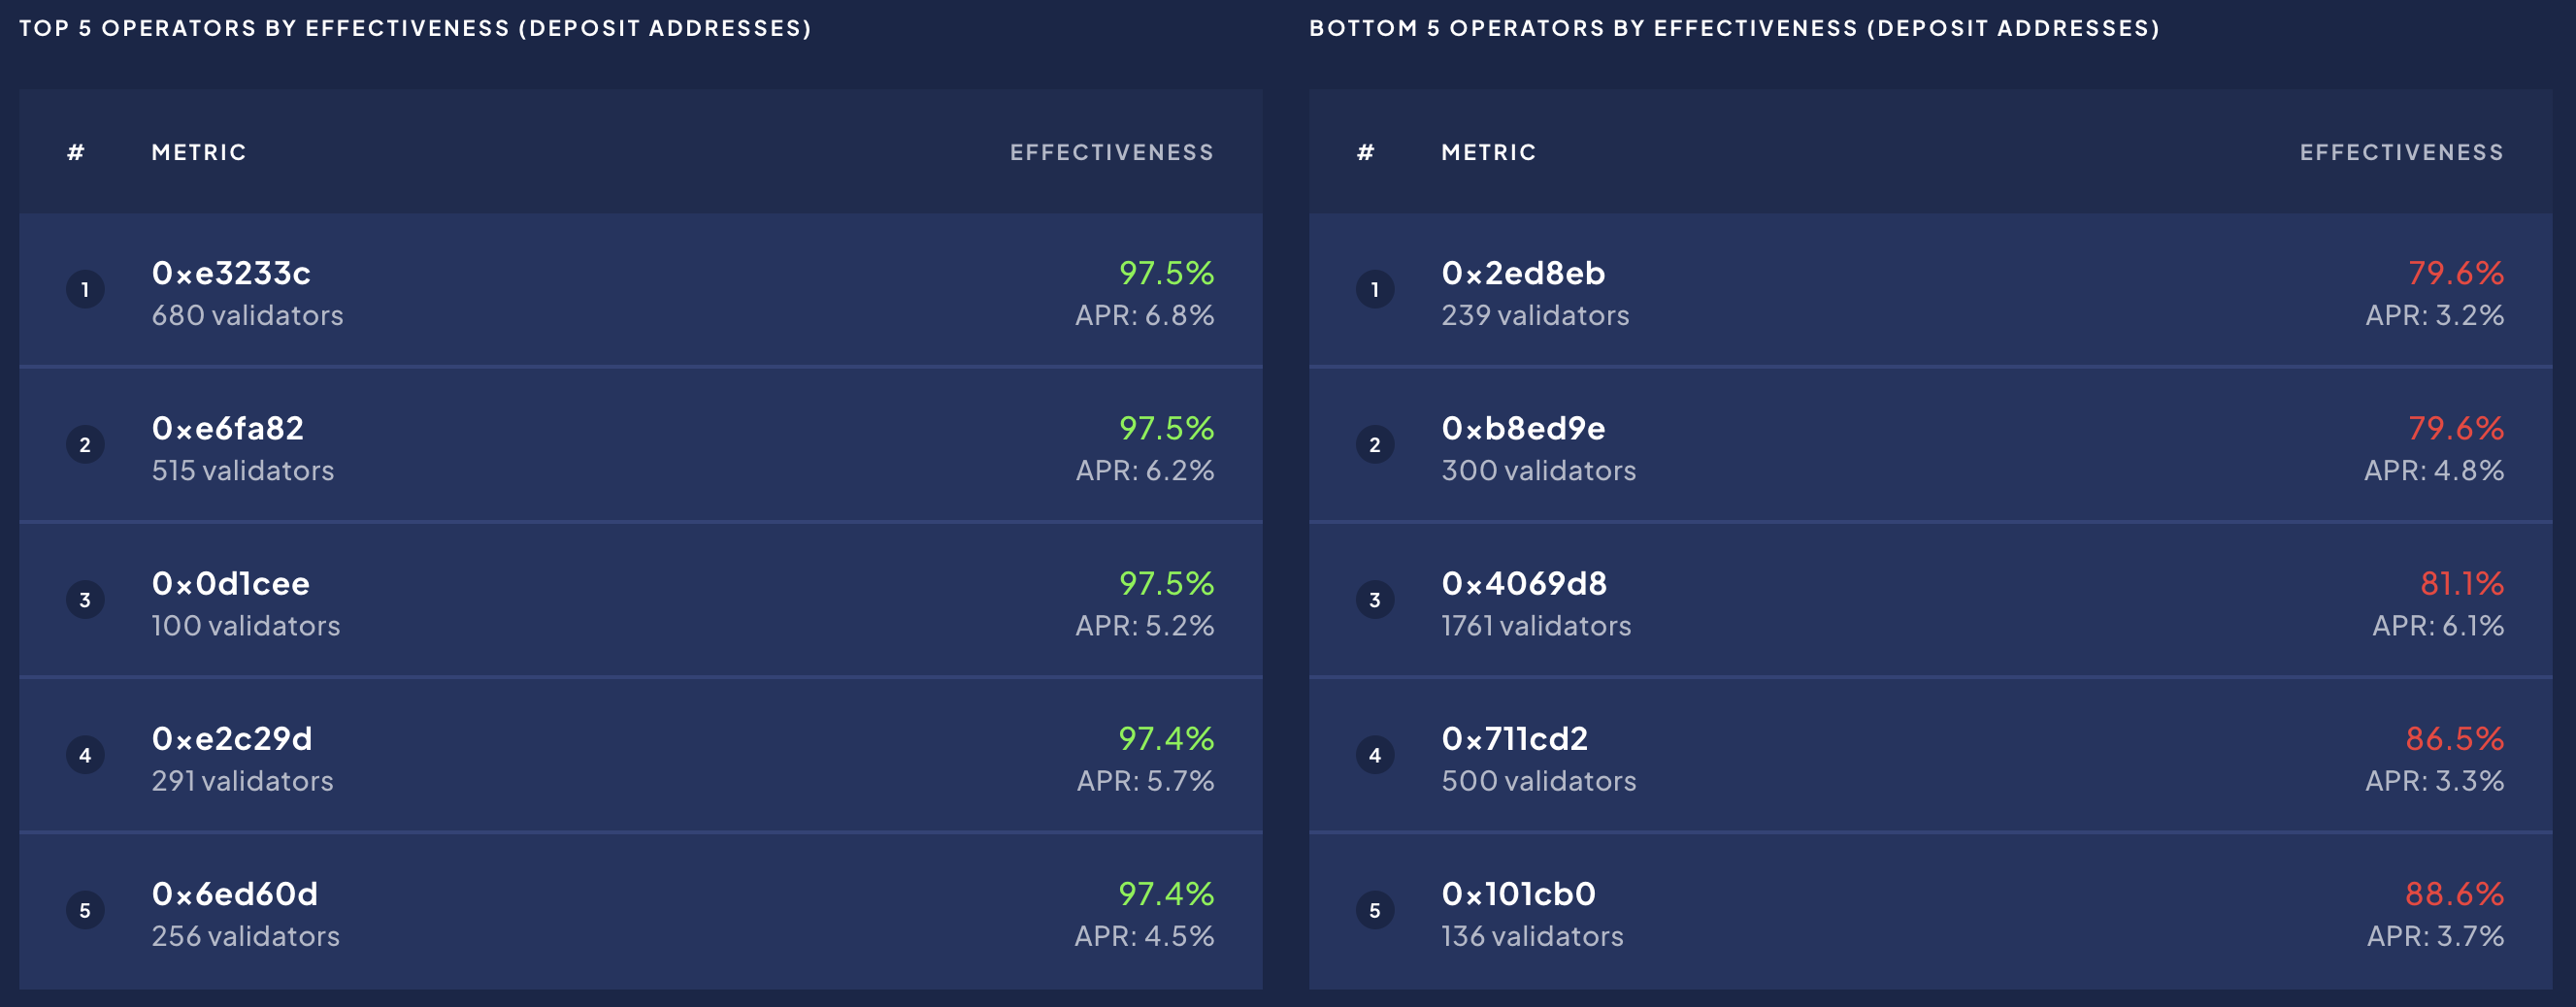
\includegraphics[width=\linewidth]{../images/ratedtrend2}\\
%(b)
%\caption{Rated network explorer: top 5 and bottom 5 identified operators (a) and the top and bottom 5 operators by deposit addresses (b). Timeframes: 1 day, 7 days, 30 days or all (since merge), 1 June 2023}
%\label{fig:ratedtrend1}
%\end{center}
%\end{figure}
%
%\begin{figure}[htbp]
%\begin{center}
%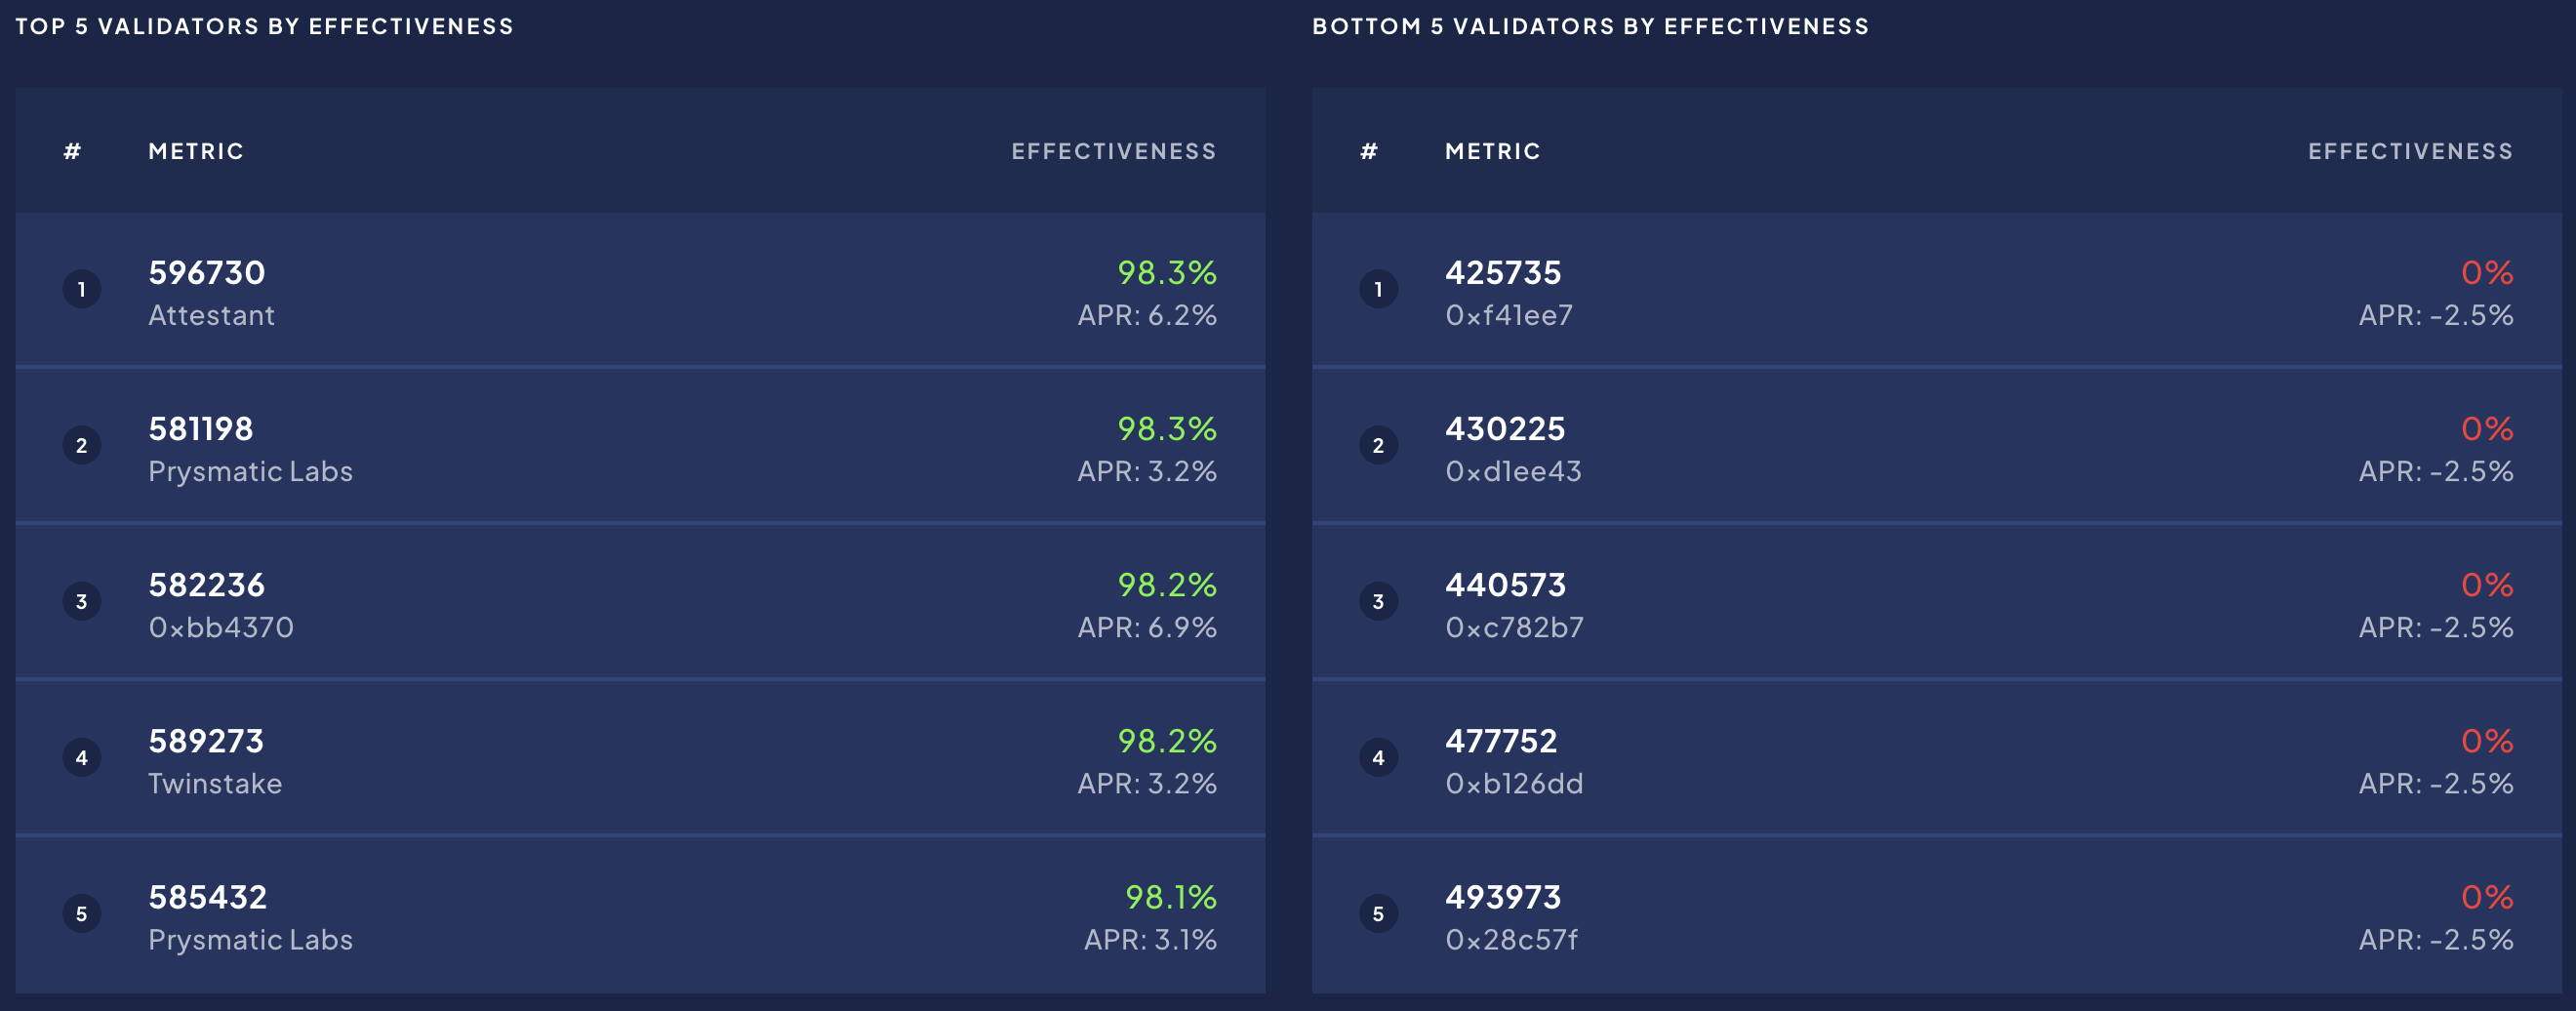
\includegraphics[width=\linewidth]{../images/ratedtrend3}\\
%(a)
%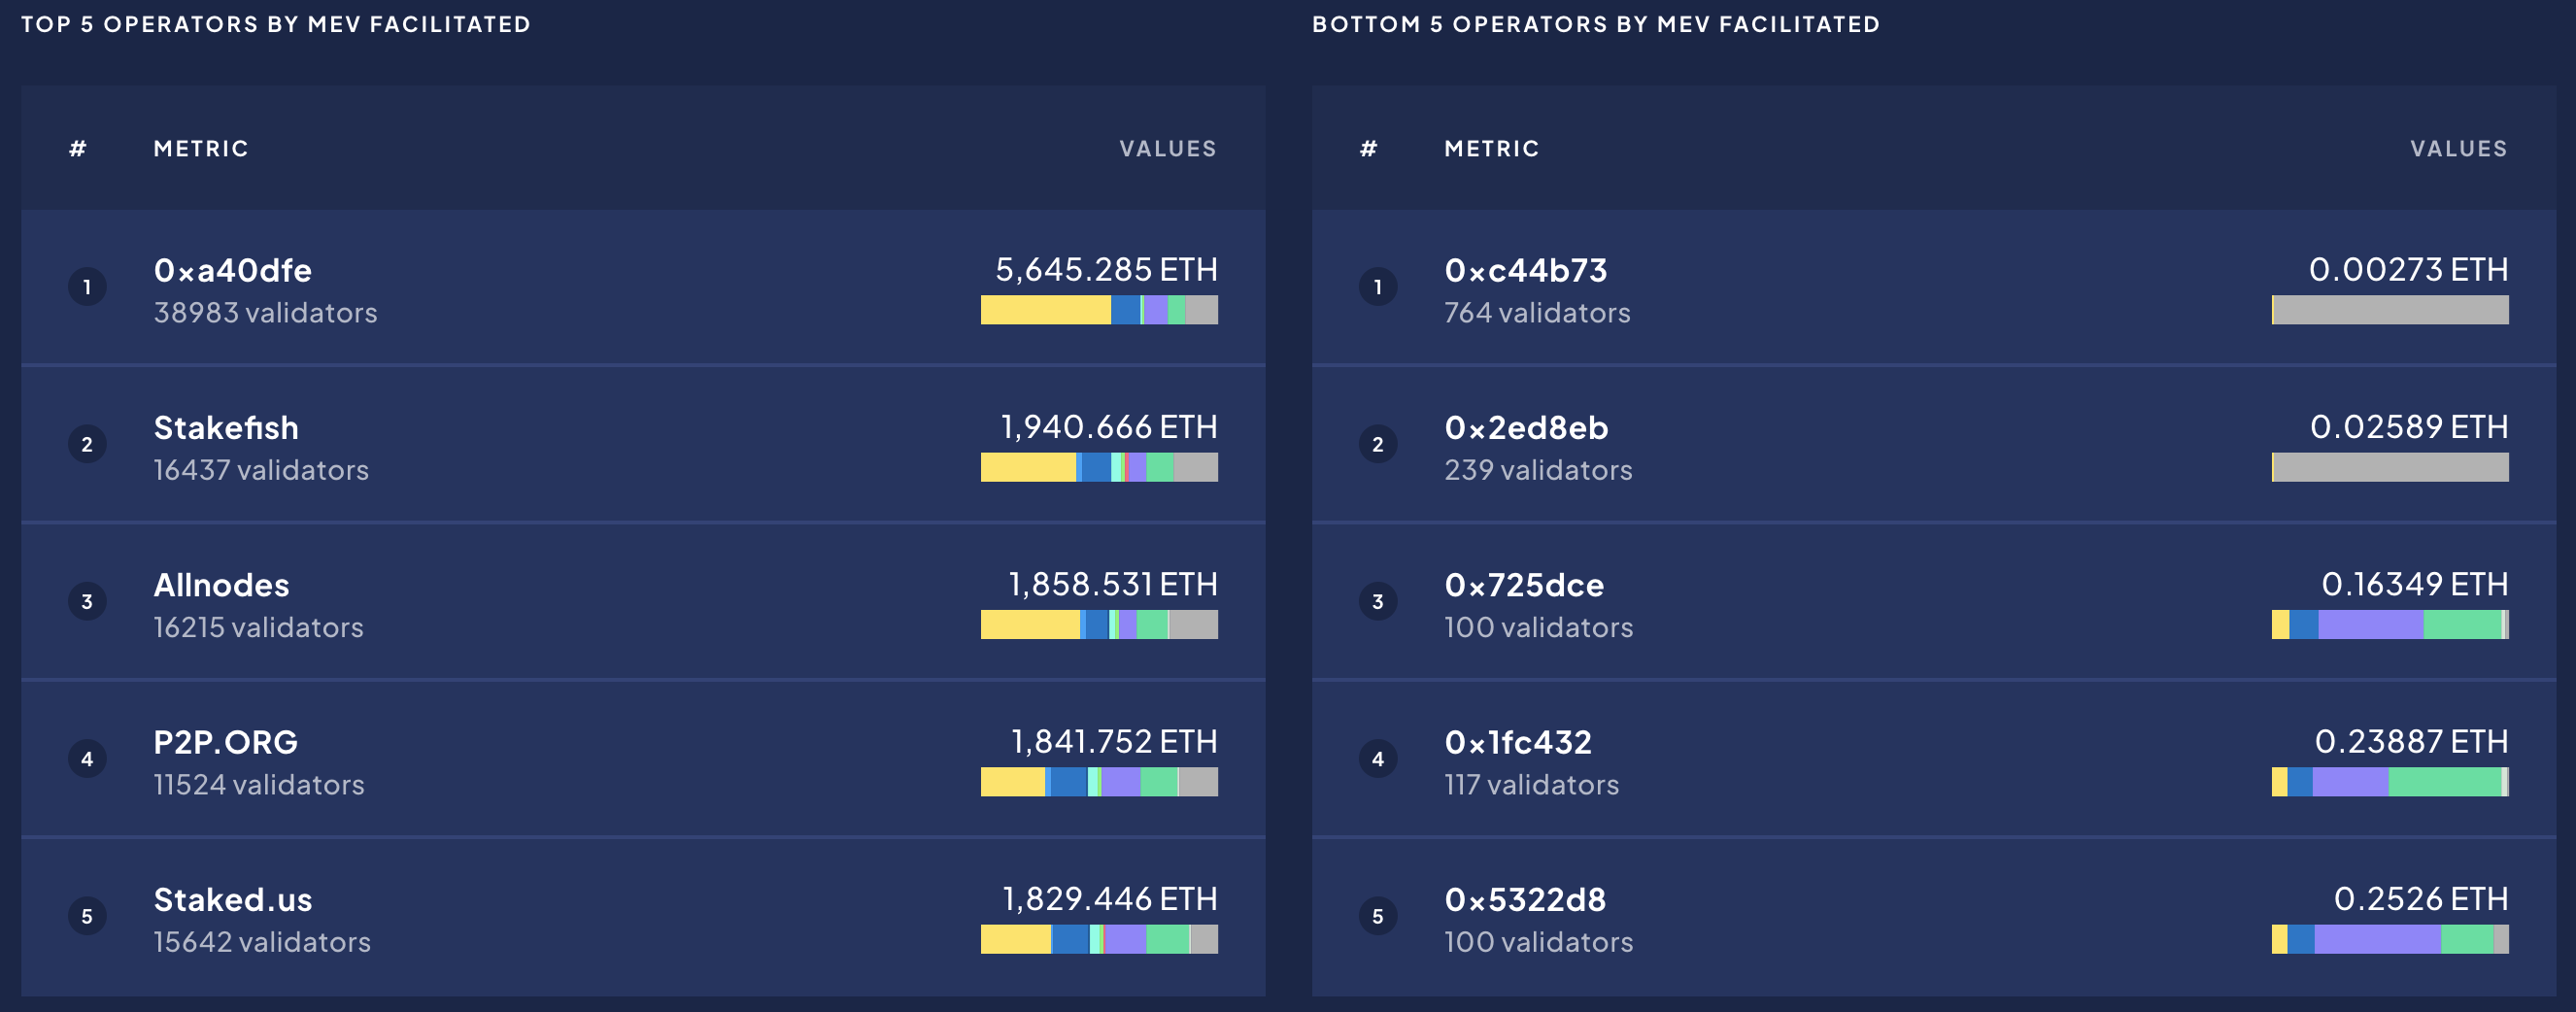
\includegraphics[width=\linewidth]{../images/ratedtrend4}\\
%(b)
%\caption{Rated network explorer: top 5 and bottom 5 validators (a).  Top 5 and bottom 5 of operators that facilitated some MEV (total or average) (b), For both visualisations, select a timeframe: 1 day, 7 days, 30 days or all (since merge),1 June 2023}
%\label{fig:ratedtrend4}
%\end{center}
%\end{figure}
%
%\begin{figure}[htbp]
%\begin{center}
%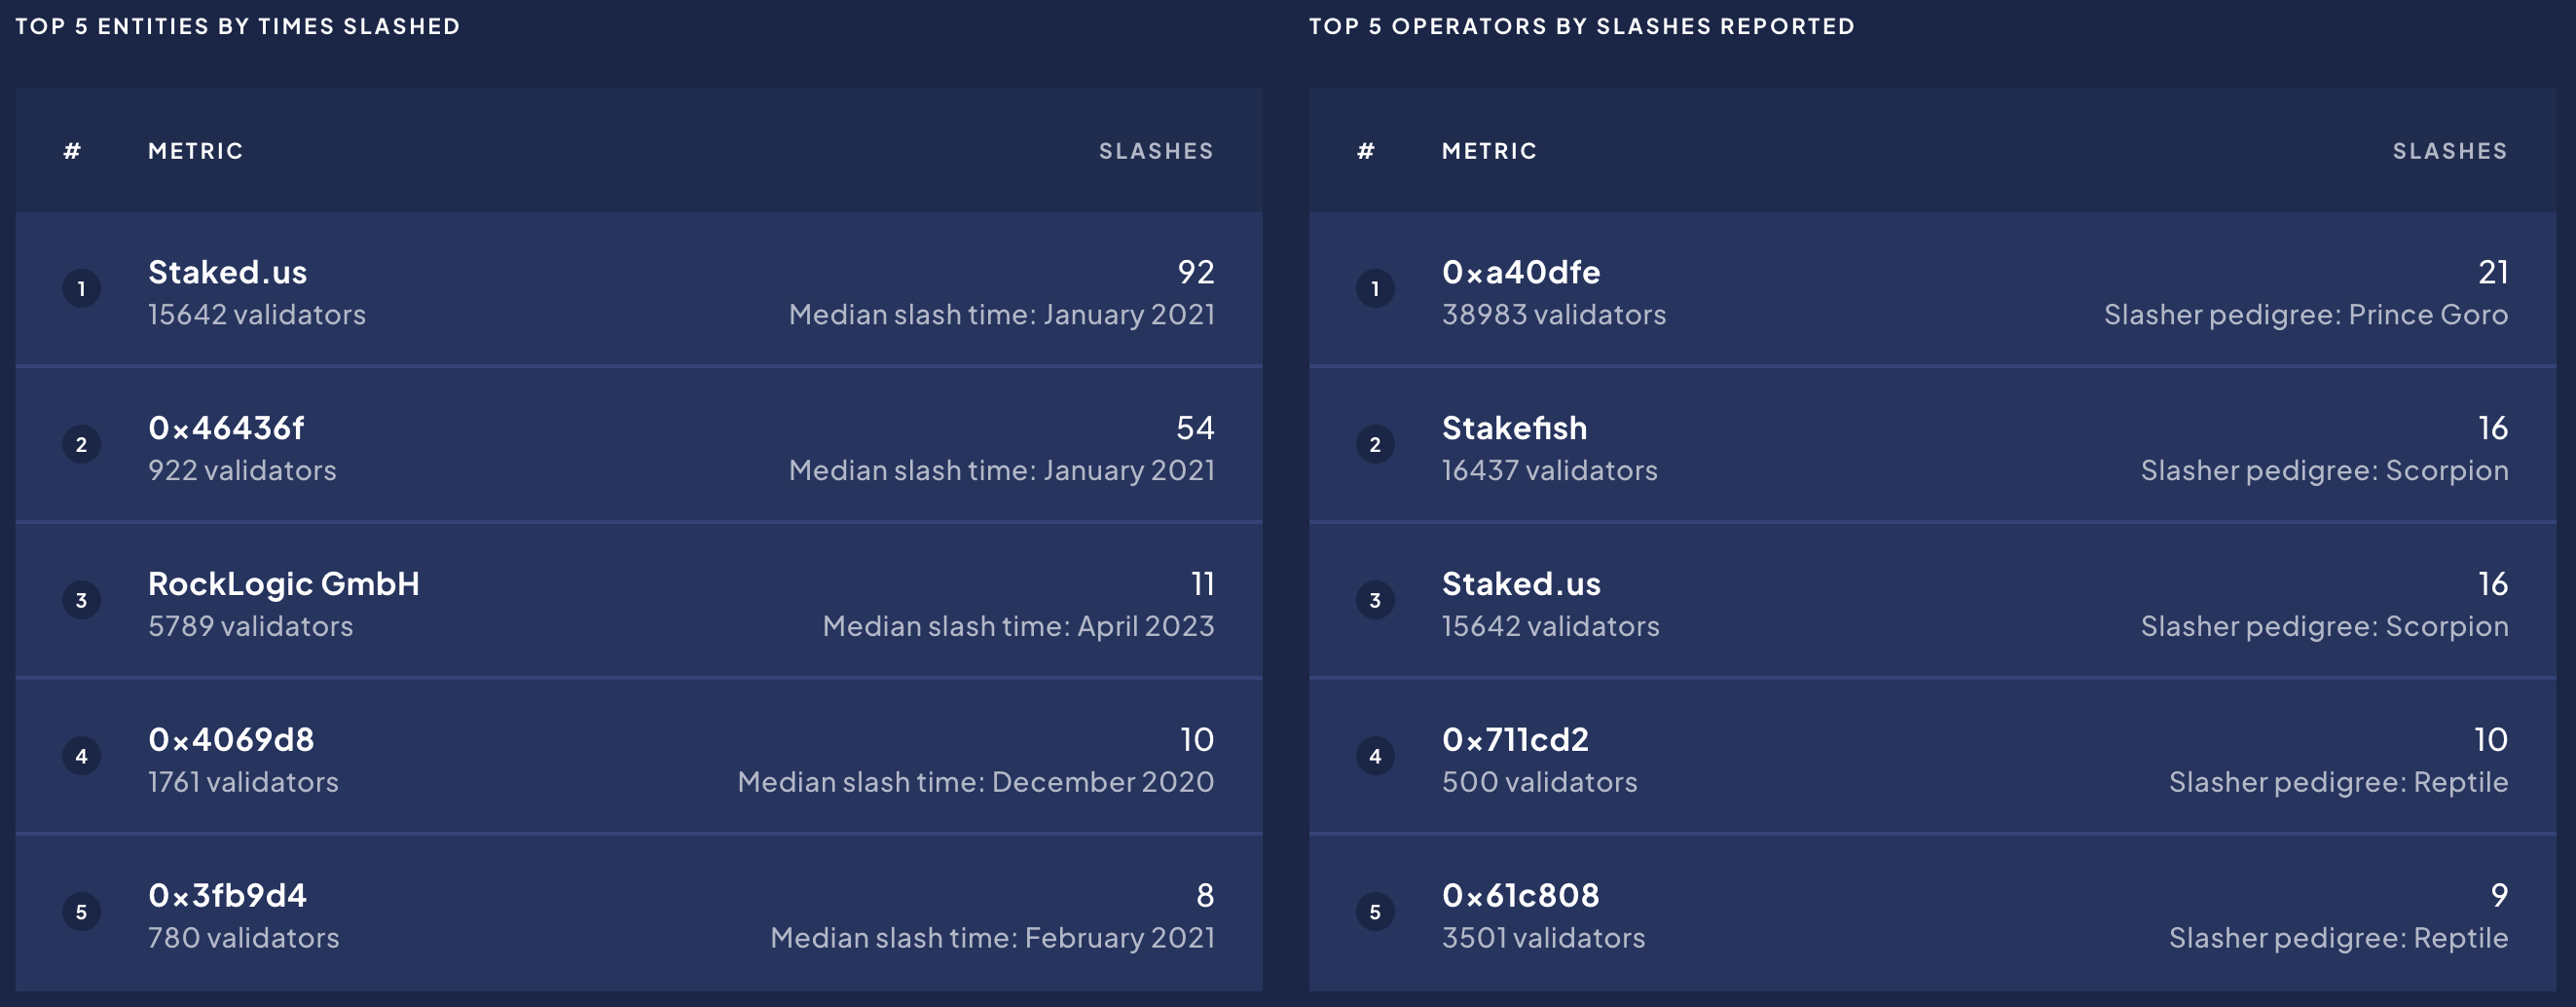
\includegraphics[width=\linewidth]{../images/ratedtrend5}
%\caption{Rated network explorer: top 5 entities by times slashed and top 5 operators by number of slashes reported. Select timeframes of 30 days, or all days (since merge) , 1 June 2023}
%\label{fig:ratedtrend5}
%\end{center}
%\end{figure}
%
%\noindent
%\textbf{Diversified Staked ETH Index (dsETH) from Index Coop}
%% ---------------------------------------
%\begin{figure}[htbp]
%\begin{center}
%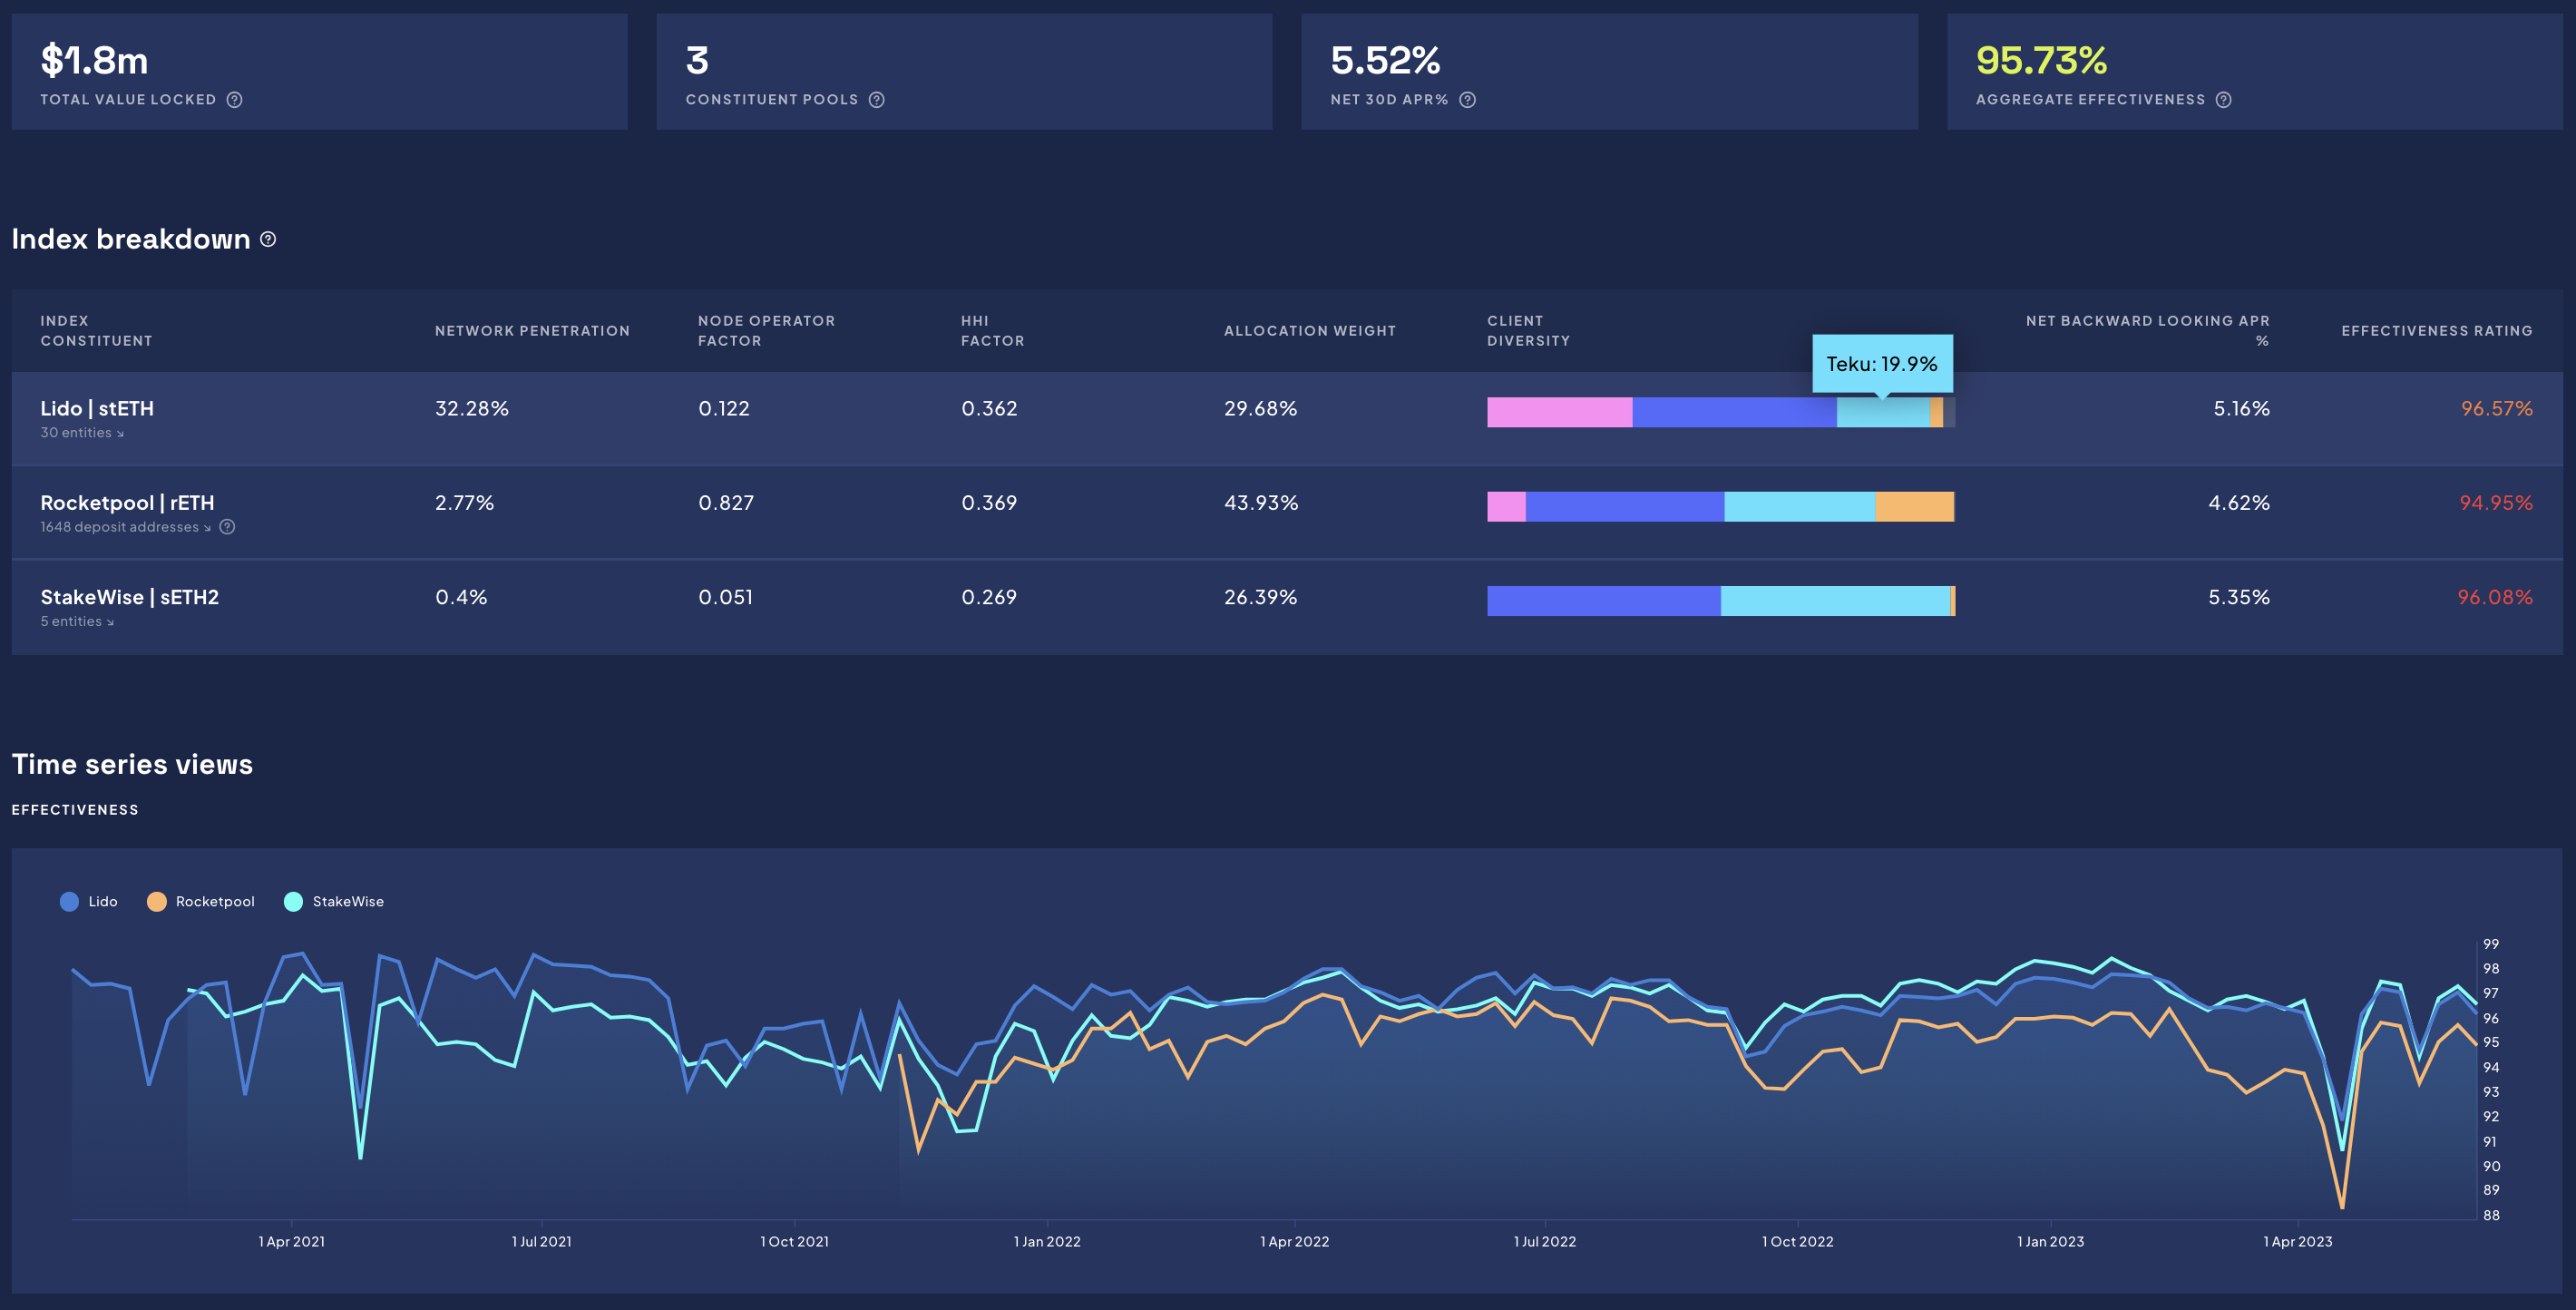
\includegraphics[width=0.9\linewidth]{../images/ratedcoop}
%\caption{Rated network explorer: Key metrics of staked ETH index and time series for all available days, selected from timeframes: 1 day, 7 days, 30 days or all (since merge), 6 June 2023}
%\label{fig:ratedcoop}
%\end{center}
%\end{figure}
%
%\clearpage
%% --------------------------------------
%\subsubsection*{Dune Analytics}
%% --------------------------------------
%\textit{\textbf{Ethereum Staking}}
%% ----------------------------------------
%\begin{figure}[htbp]
%\begin{center}
%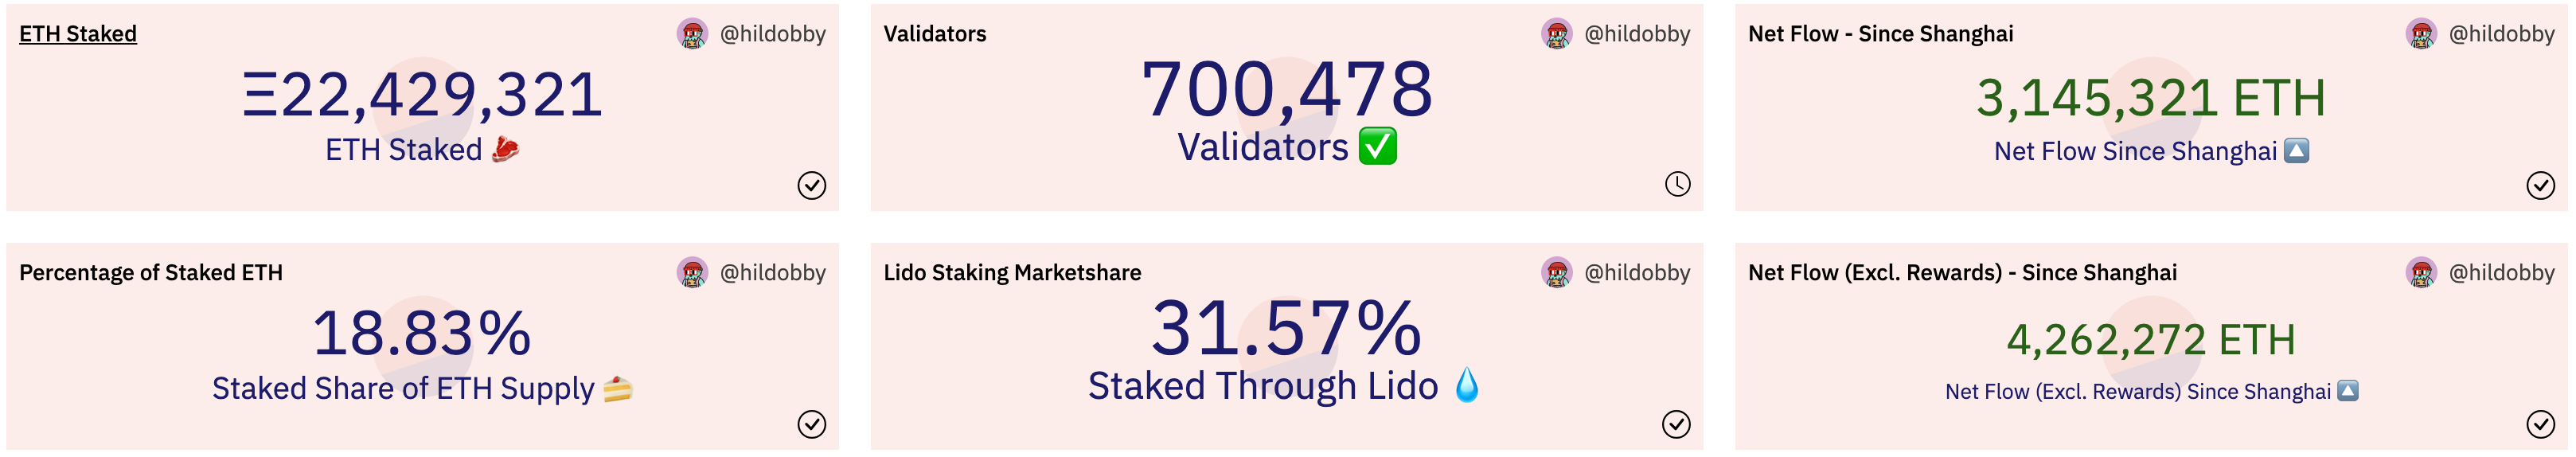
\includegraphics[width=\linewidth]{../images/hildobby1}\\
%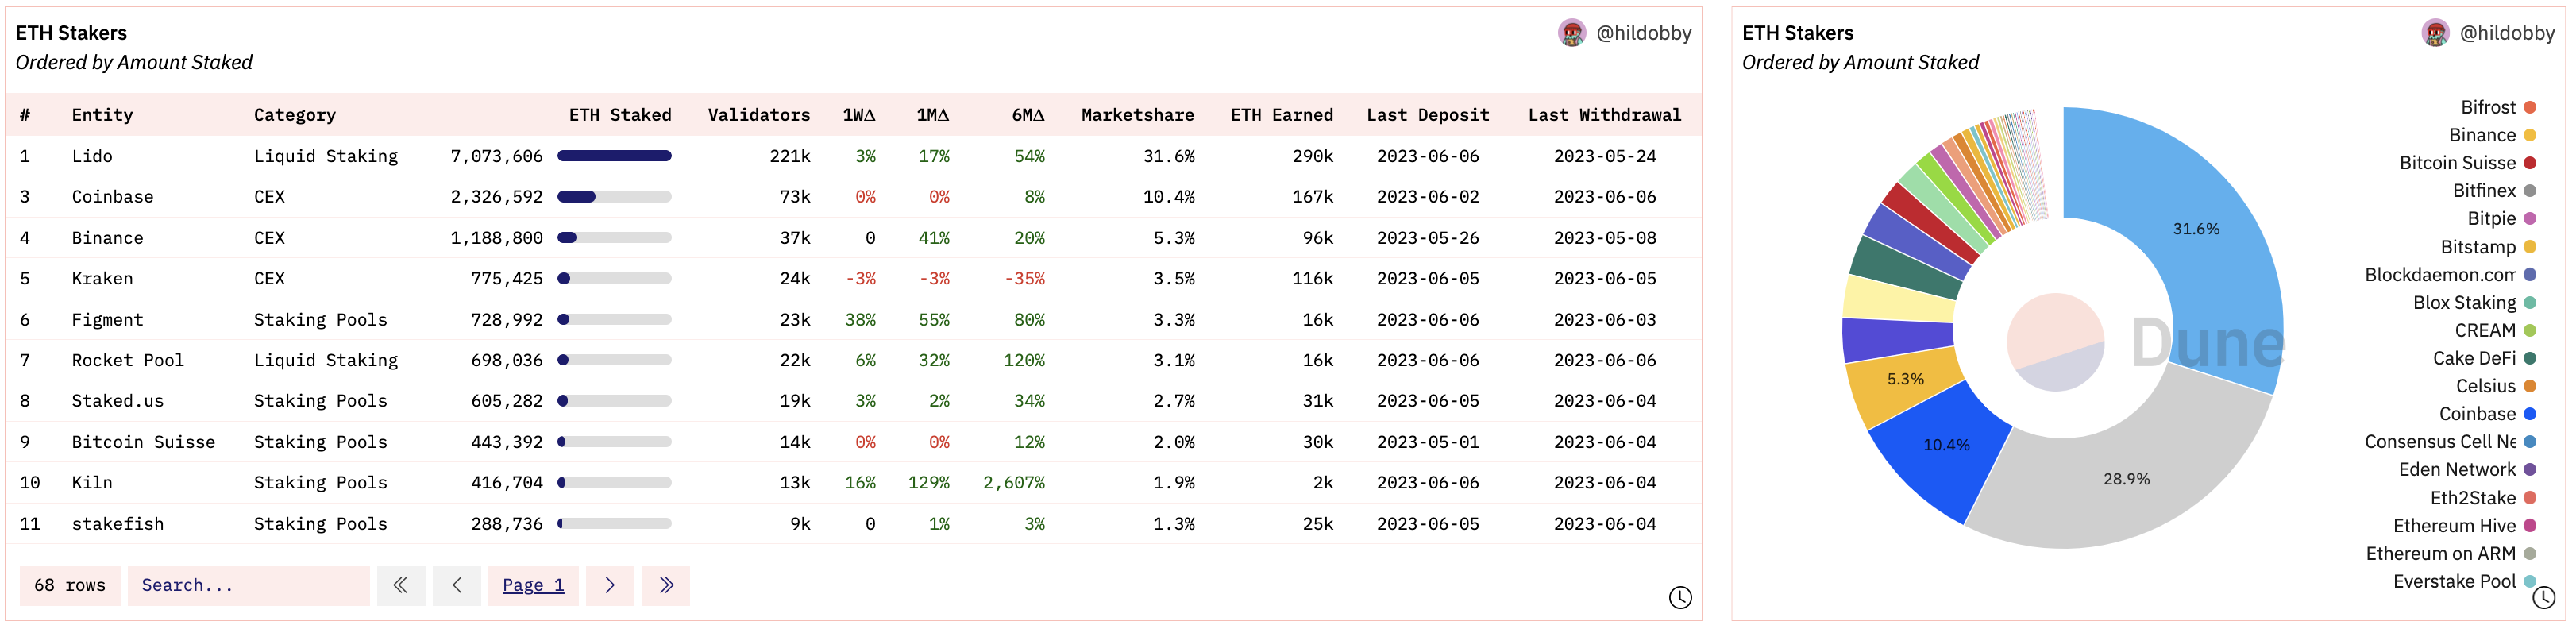
\includegraphics[width=\linewidth]{../images/hildobby2}
%\caption{Dune Analytics Ethereum staking charts. @hildobby  (7 June 2023)}
%\label{fig:hildobby1}
%\end{center}
%\end{figure}
%
%\begin{figure}[htbp]
%\begin{center}
%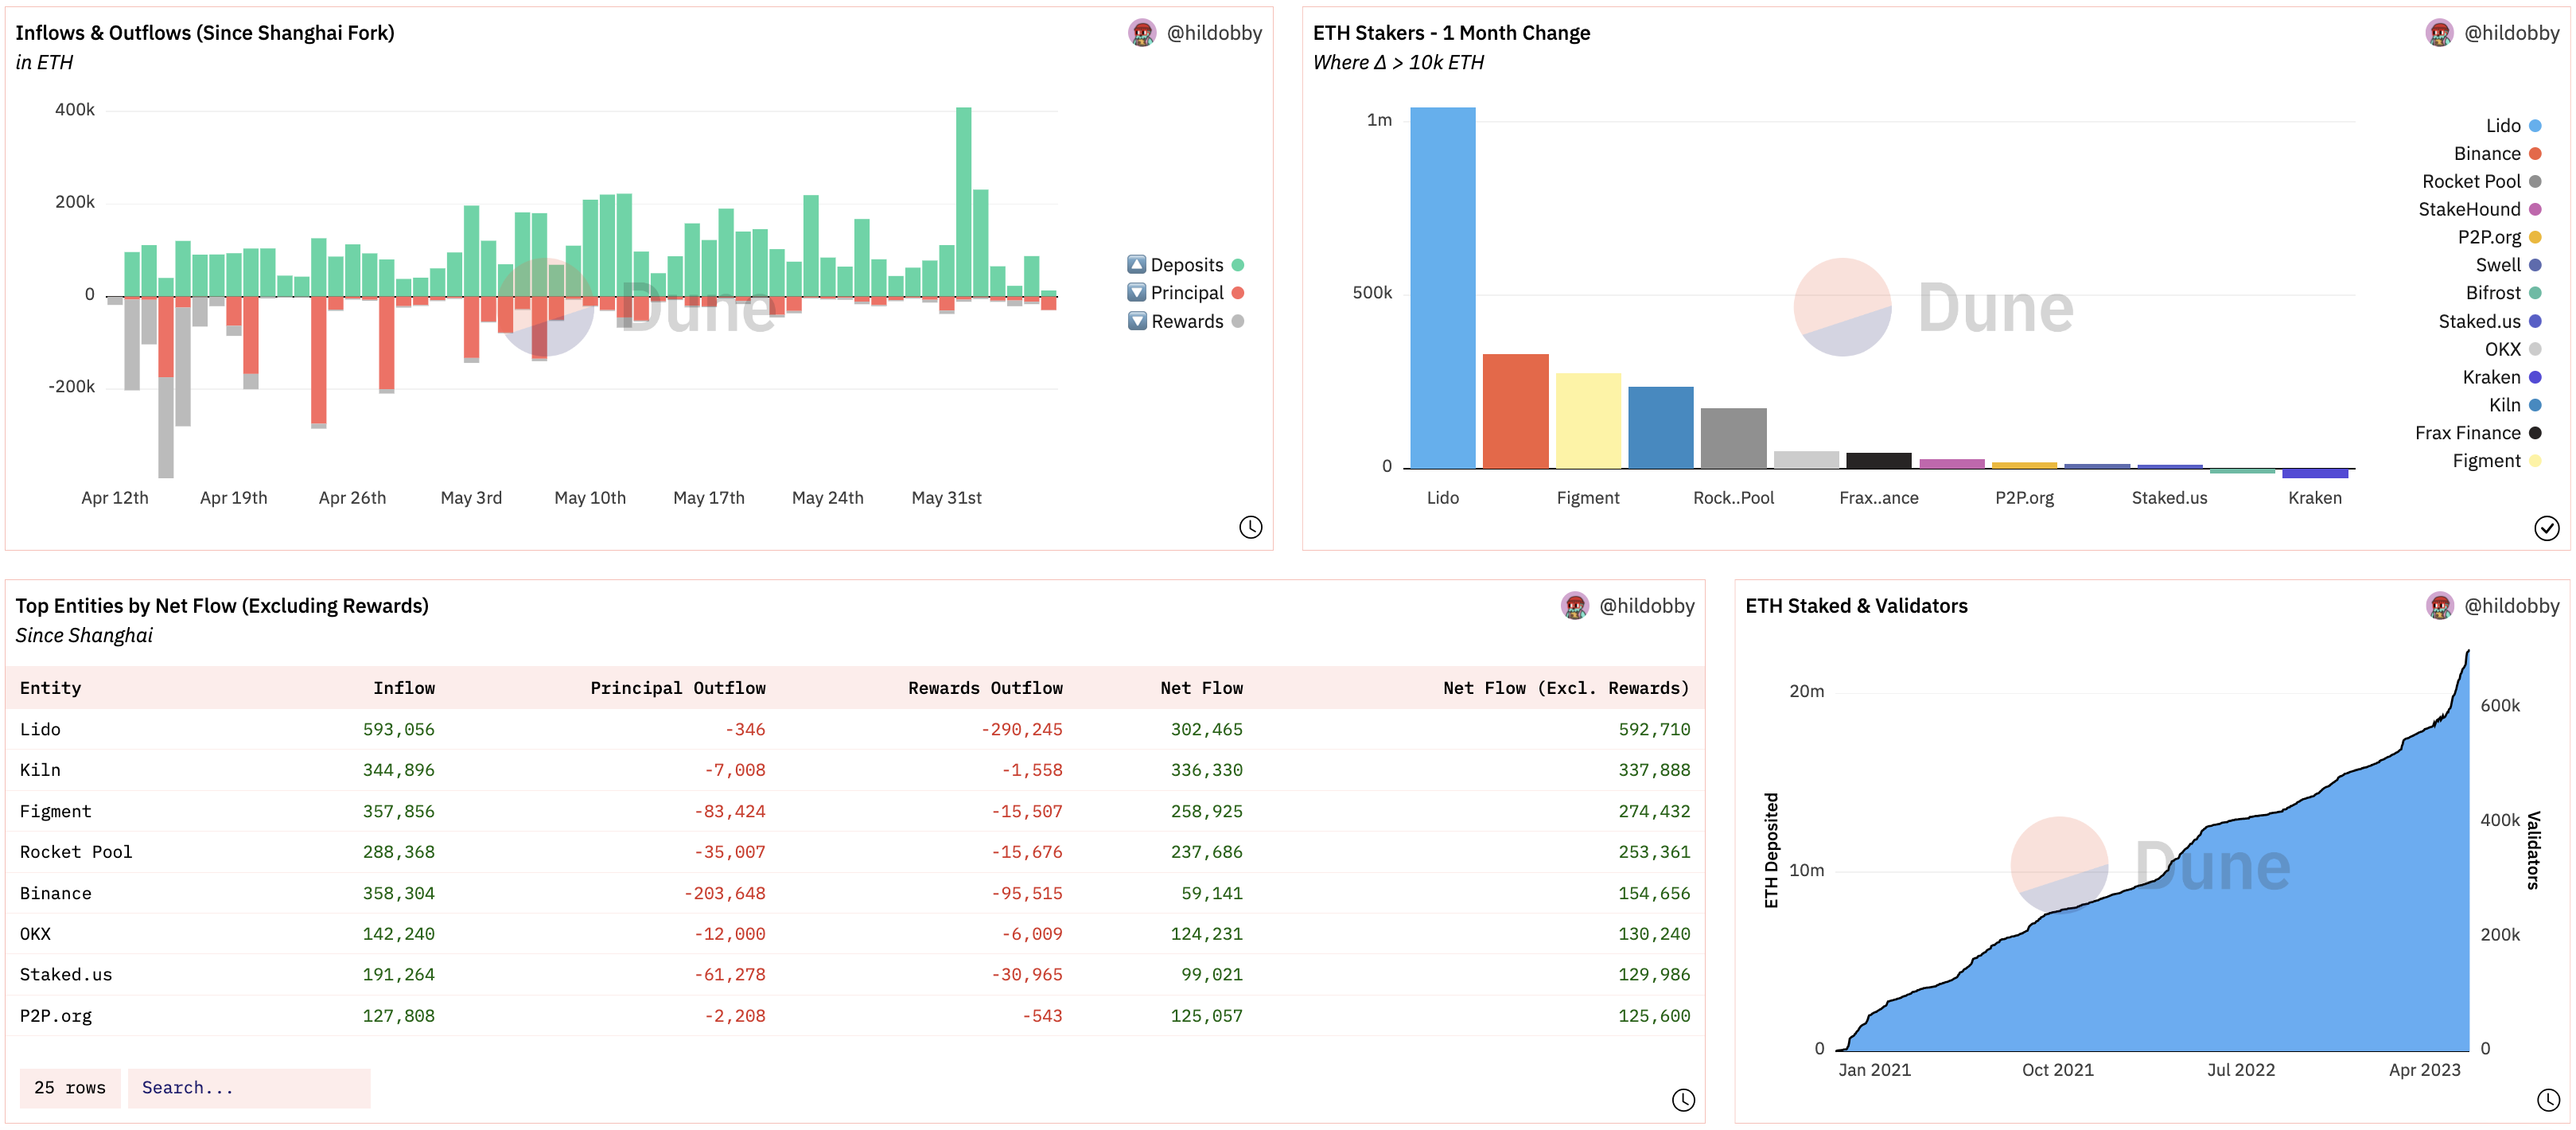
\includegraphics[width=\linewidth]{../images/hildobby3}\\
%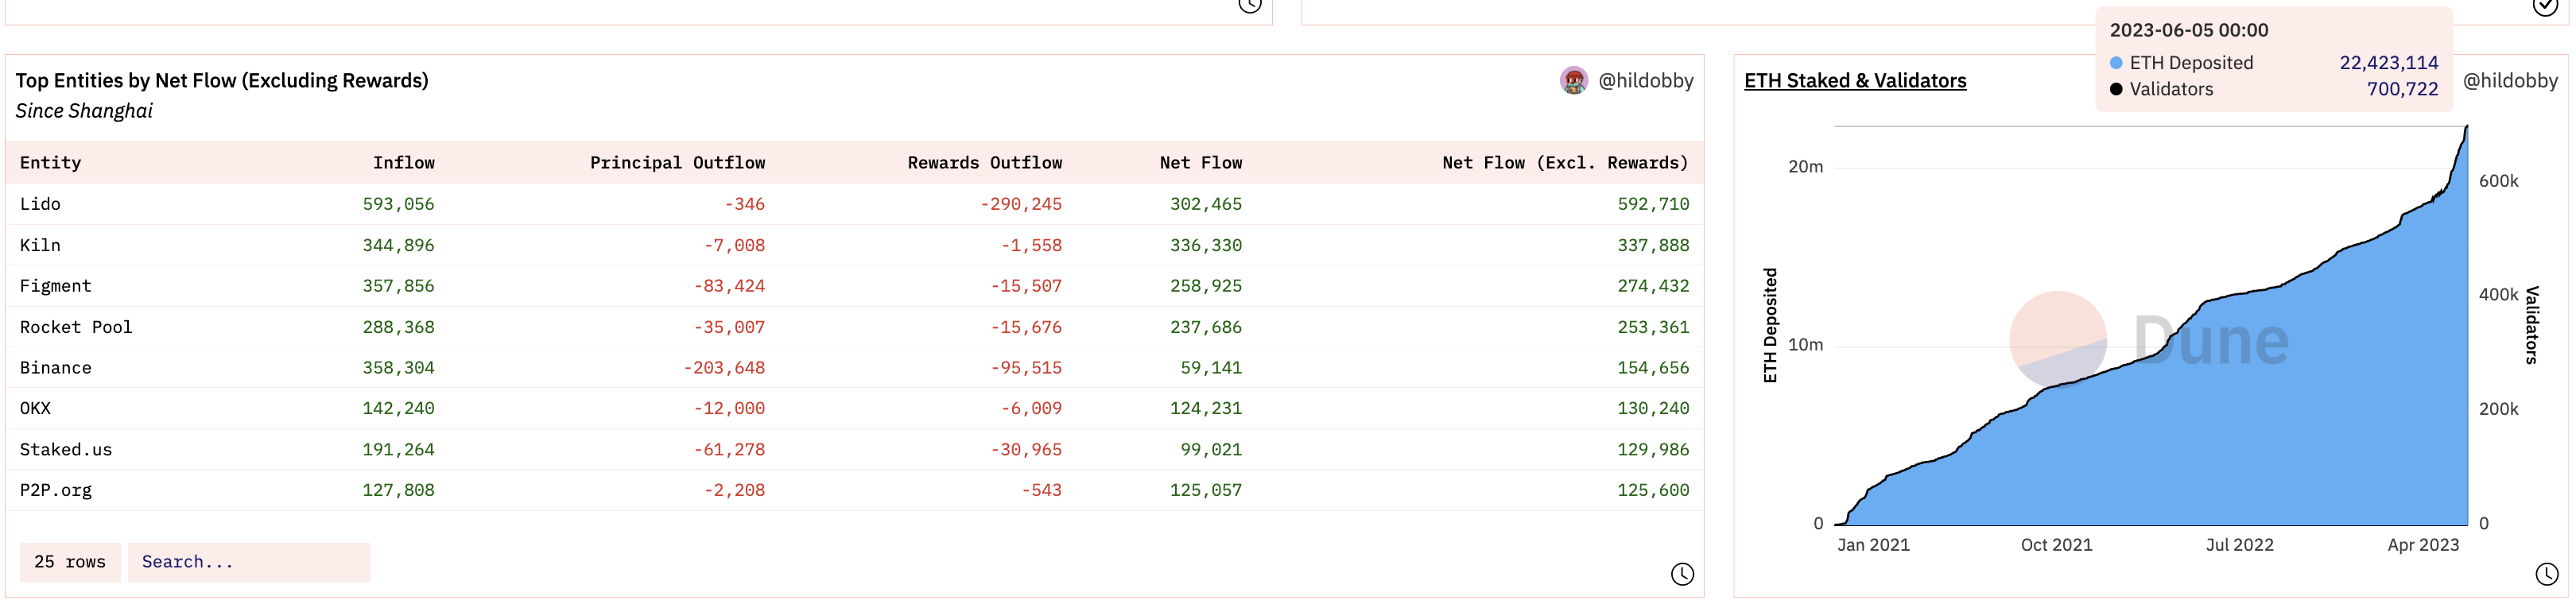
\includegraphics[width=\linewidth]{../images/hildobby4}
%\caption{Dune Analytics ETH inflows and outflows, ETH staked and validators. @hildobby  (7 June 2023)}
%\label{fig:hildobby3}
%\end{center}
%\end{figure}
%
%
%\begin{figure}[htbp]
%\begin{center}
%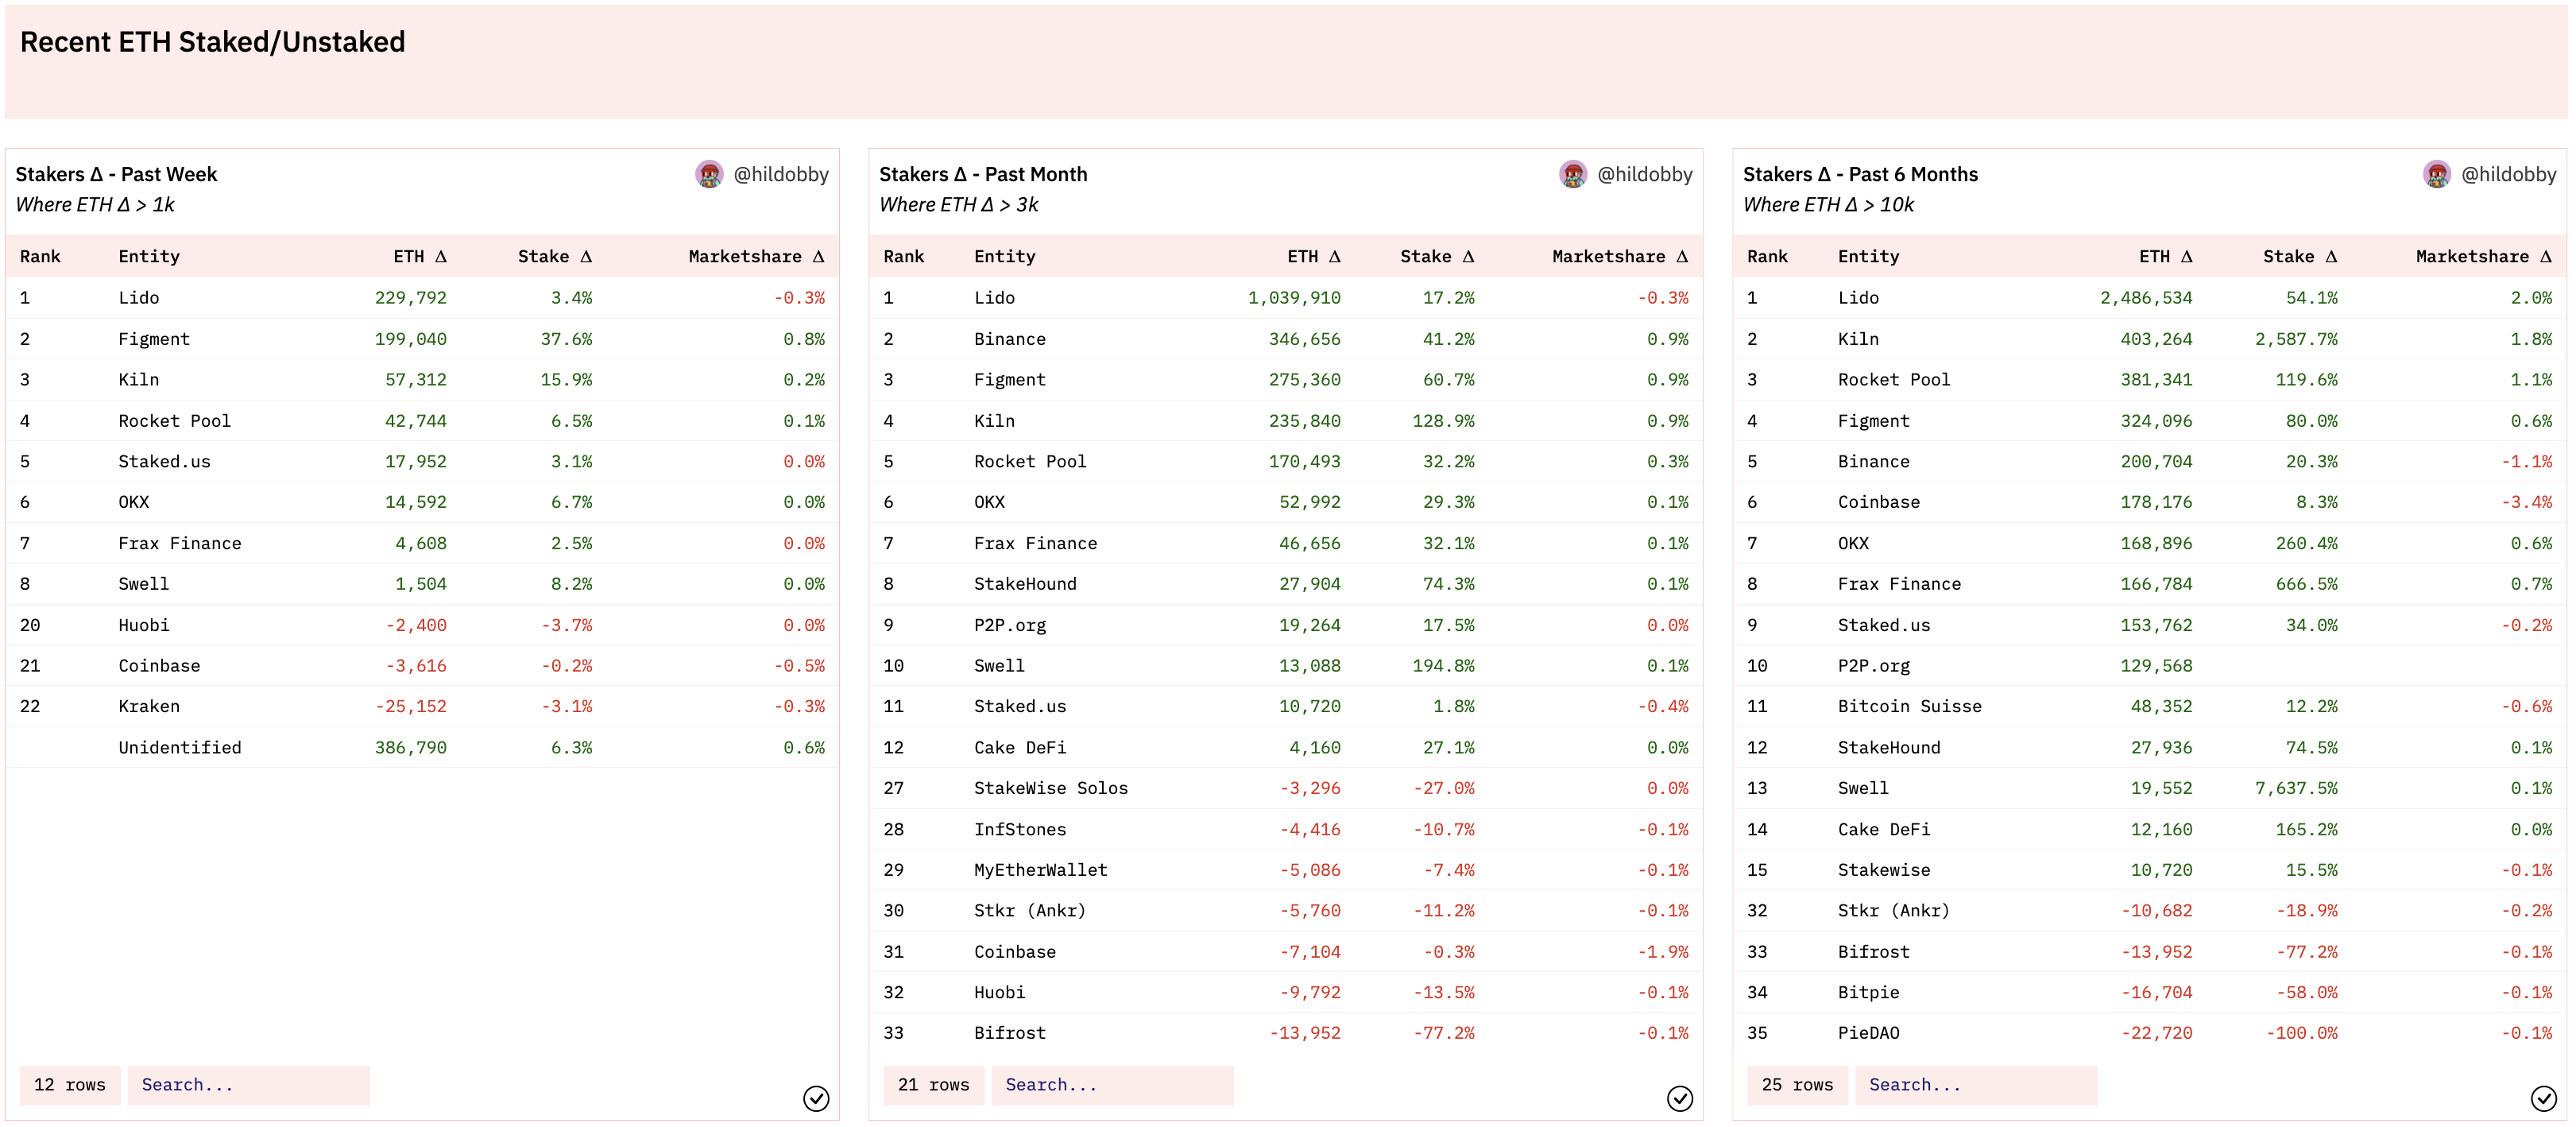
\includegraphics[width=\linewidth]{../images/hildobby5}
%\caption{Dune Analytics Recent ETH staked. @hildobby  (7 June 2023)}
%\label{fig:hildobby5}
%\end{center}
%\end{figure}
%
%\begin{figure}[htbp]
%\begin{center}
%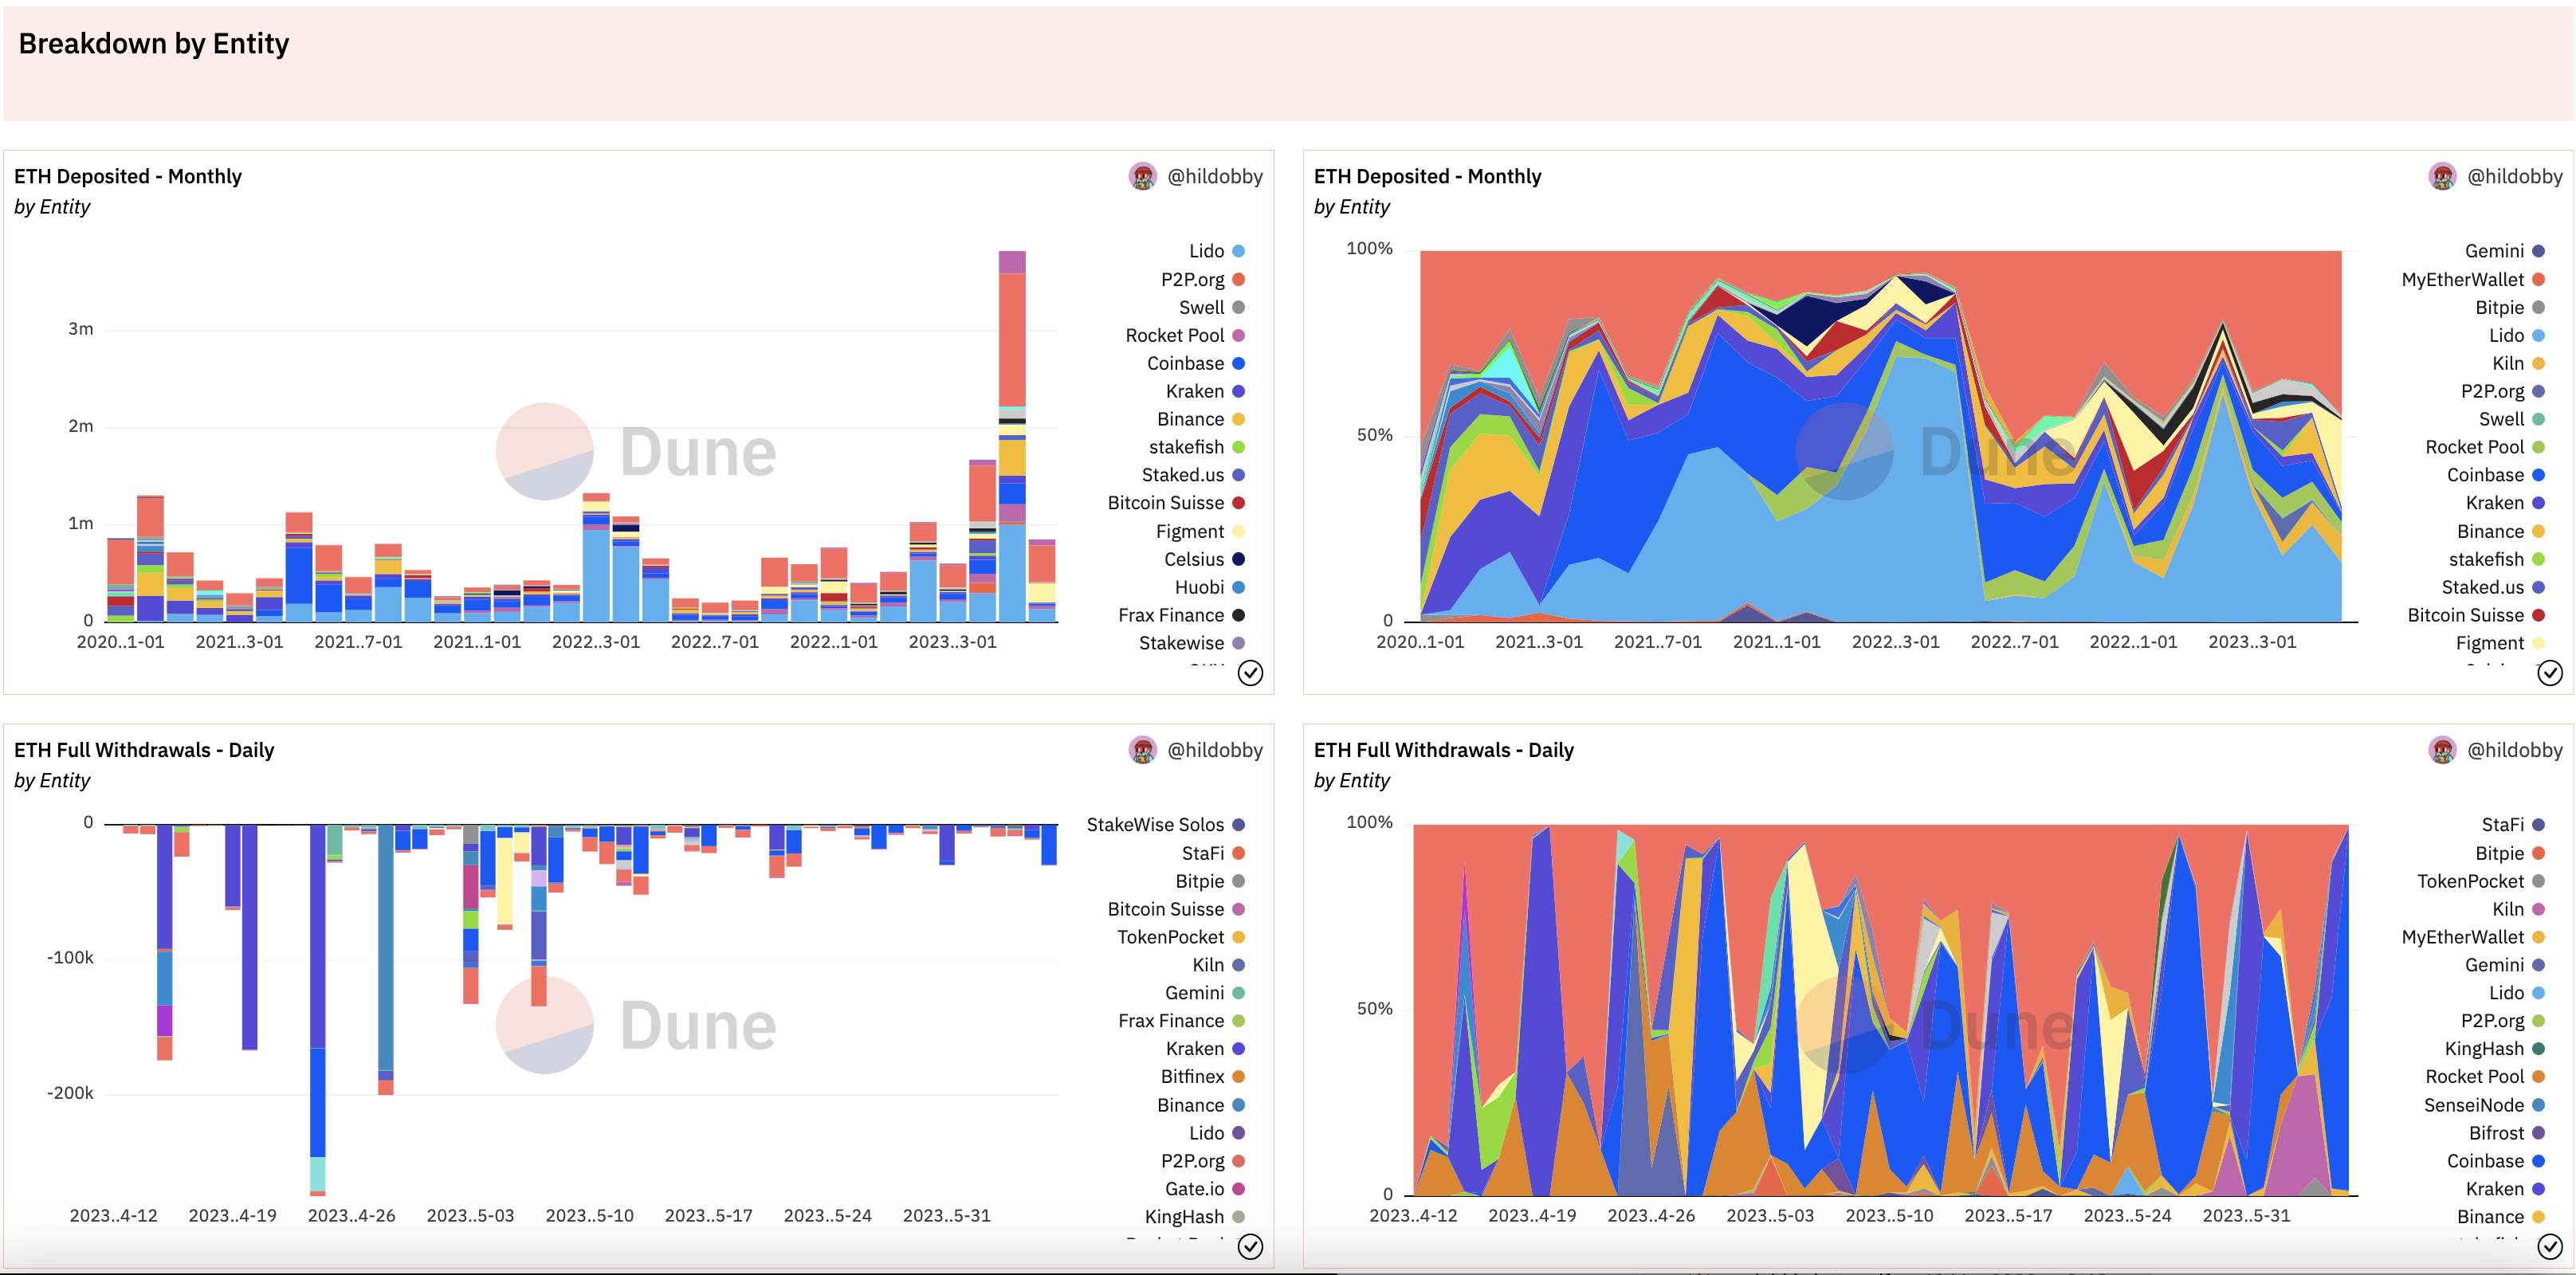
\includegraphics[width=\linewidth]{../images/hildobby6}\\
%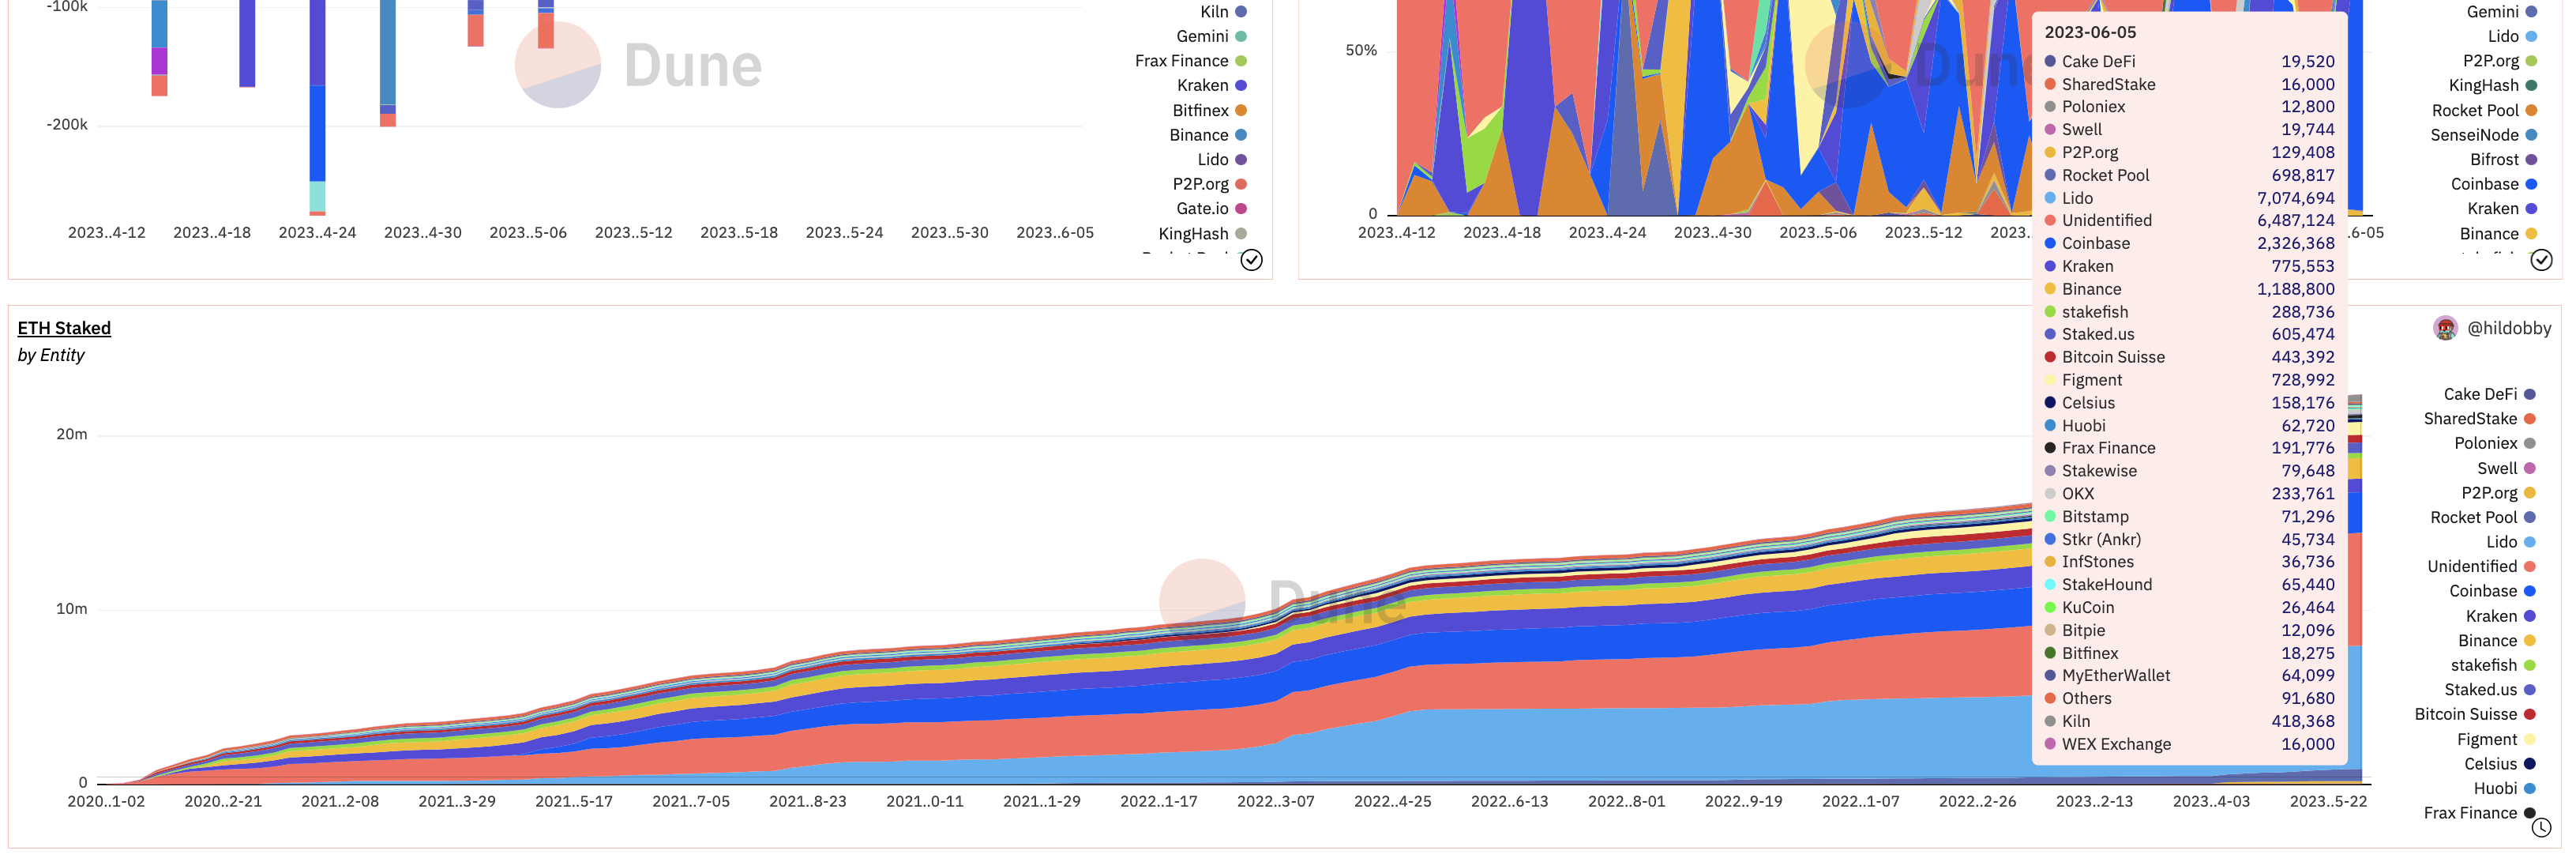
\includegraphics[width=\linewidth]{../images/hildobby7}
%\caption{Dune Analytics ETH staked and withdrawn by entity. @hildobby  (7 June 2023)}
%\label{fig:hildobby6}
%\end{center}
%\end{figure}
%
%\begin{figure}[htbp]
%\begin{center}
%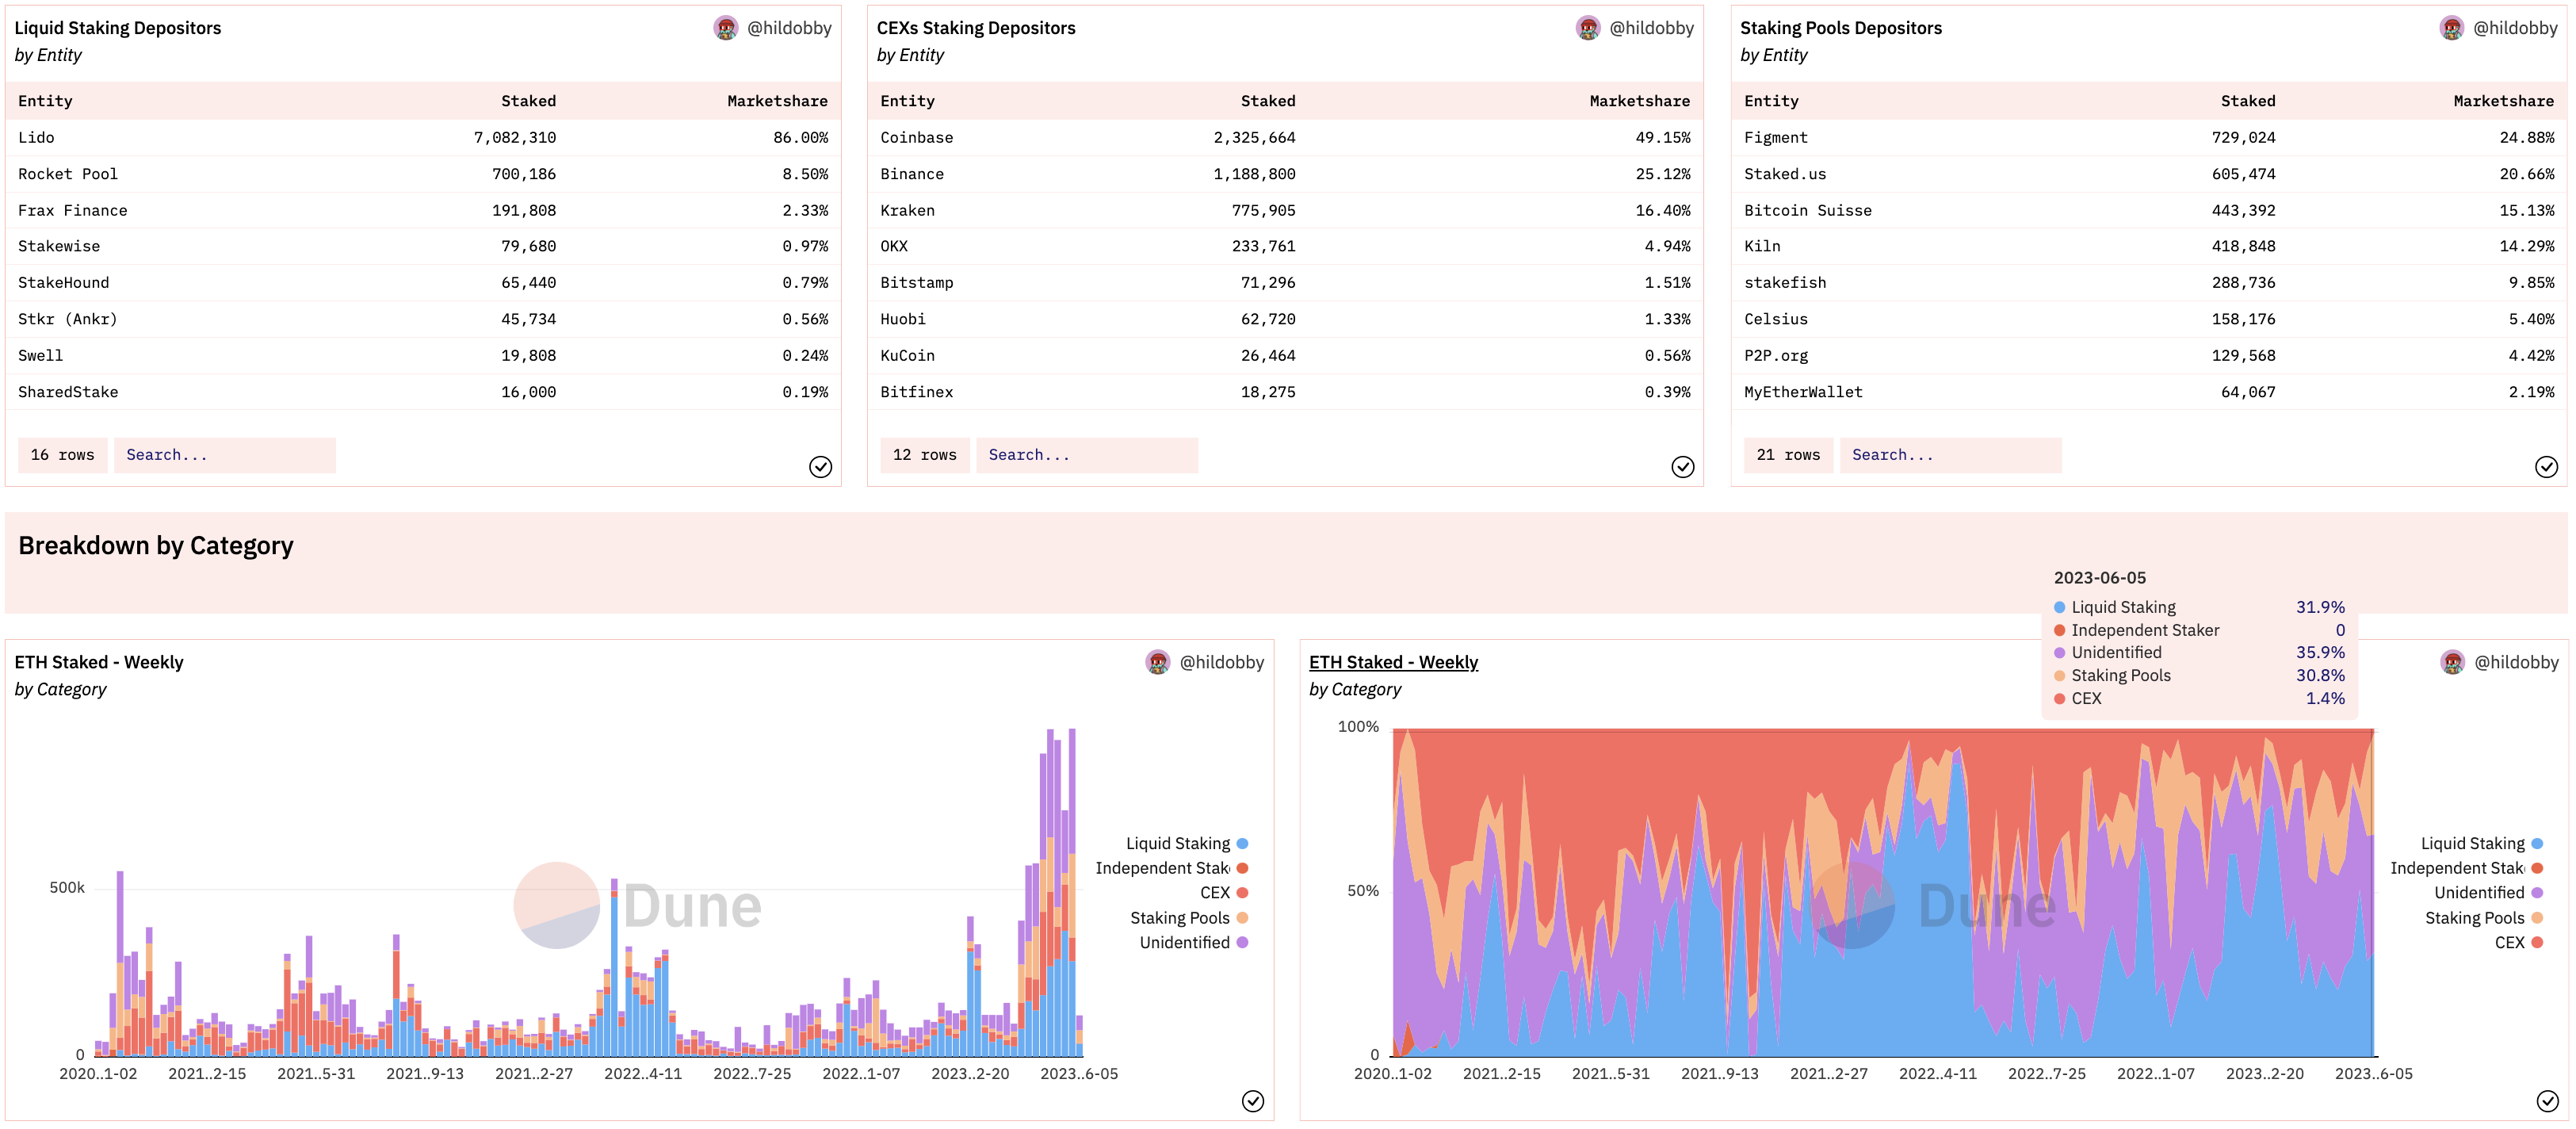
\includegraphics[width=\linewidth]{../images/hildobby8}\\
%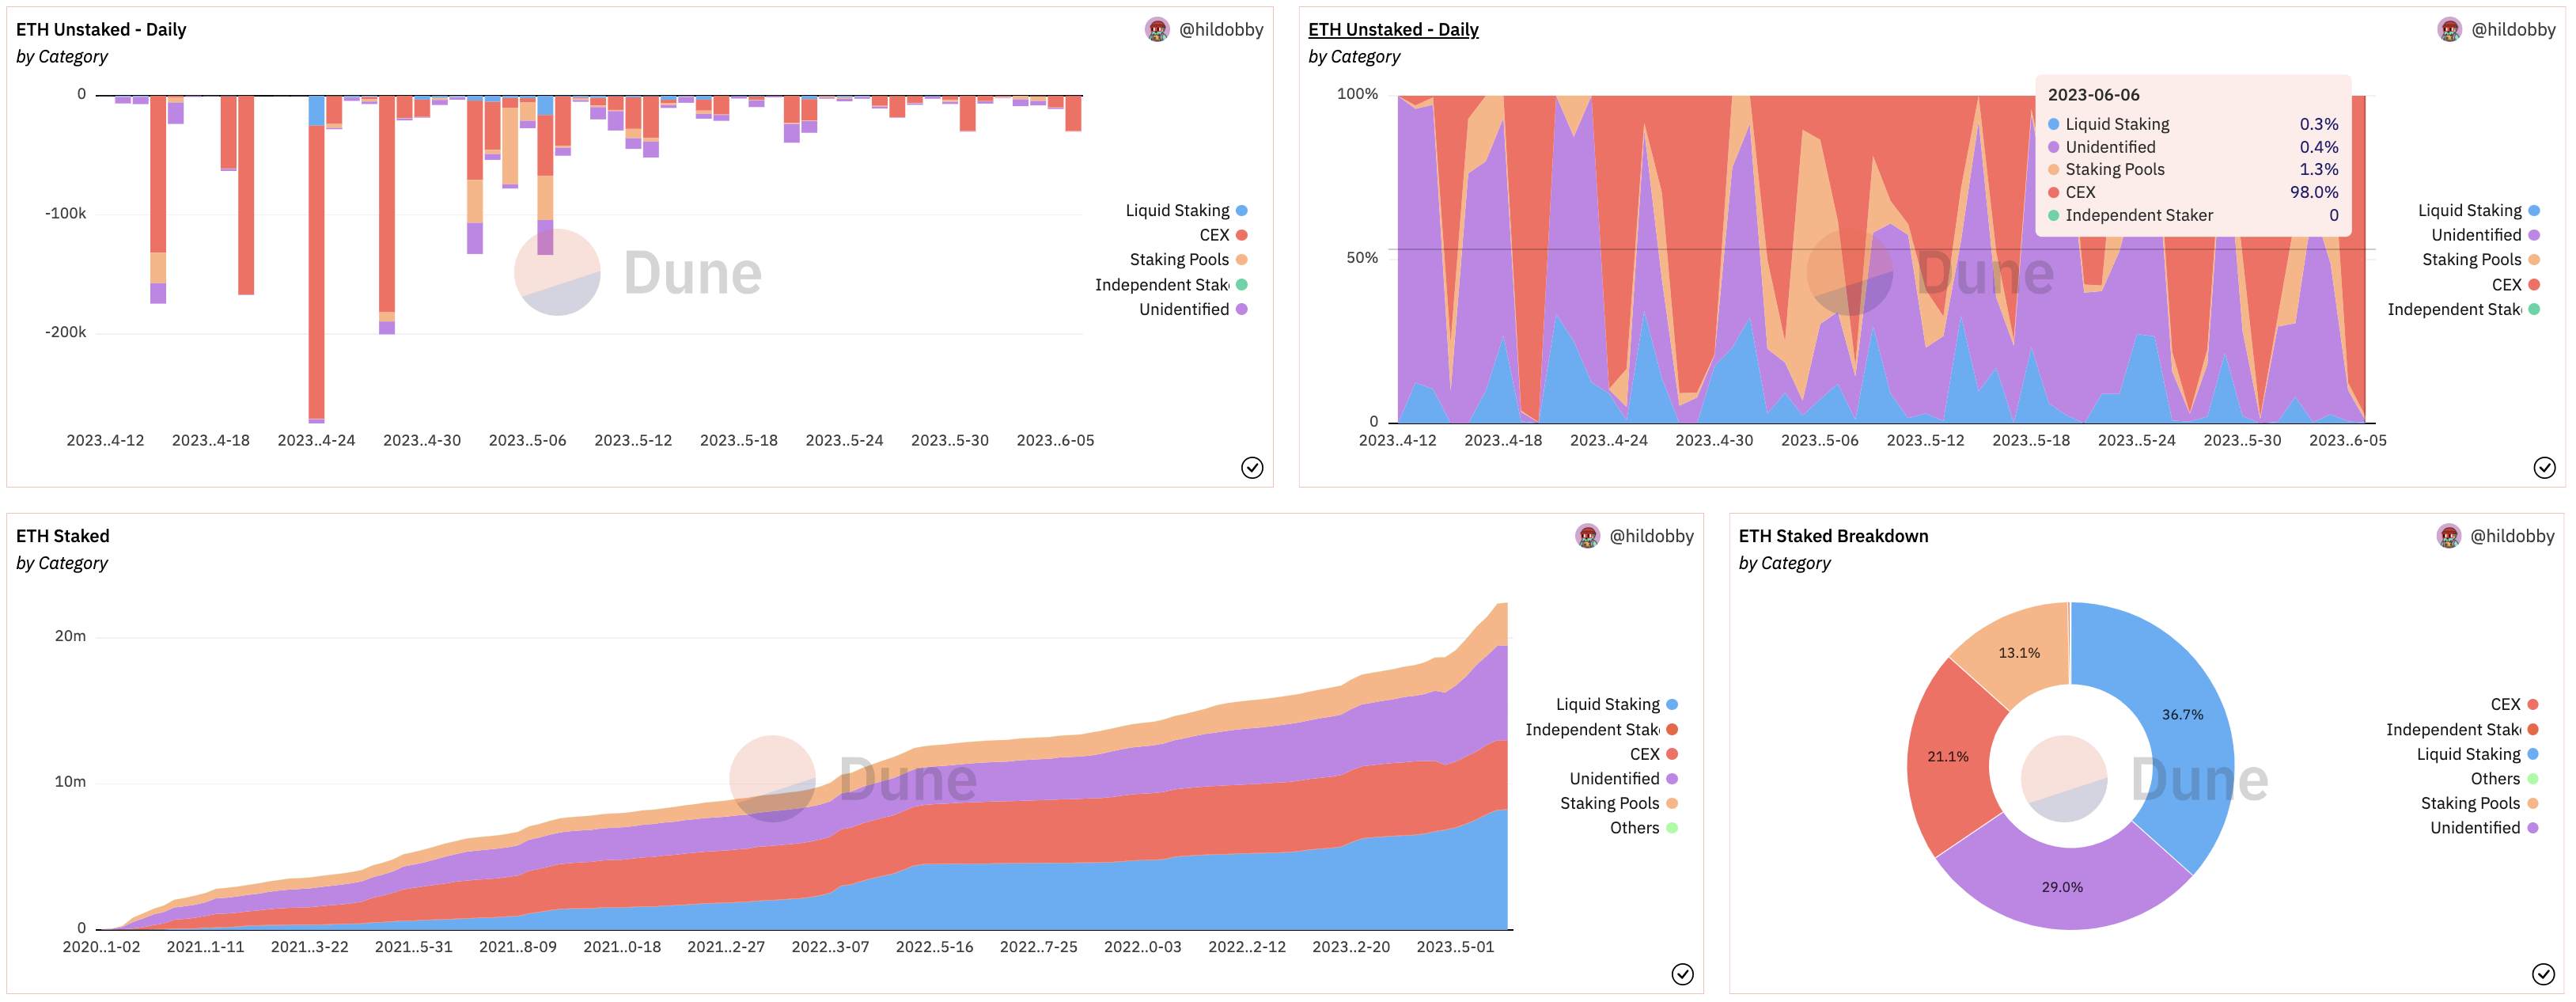
\includegraphics[width=\linewidth]{../images/hildobby9}
%\caption{Dune Analytics ETH staked by entity and category. @hildobby  (7 June 2023)}
%\label{fig:hildobby8}
%\end{center}
%\end{figure}
%
%\begin{figure}[htbp]
%\begin{center}
%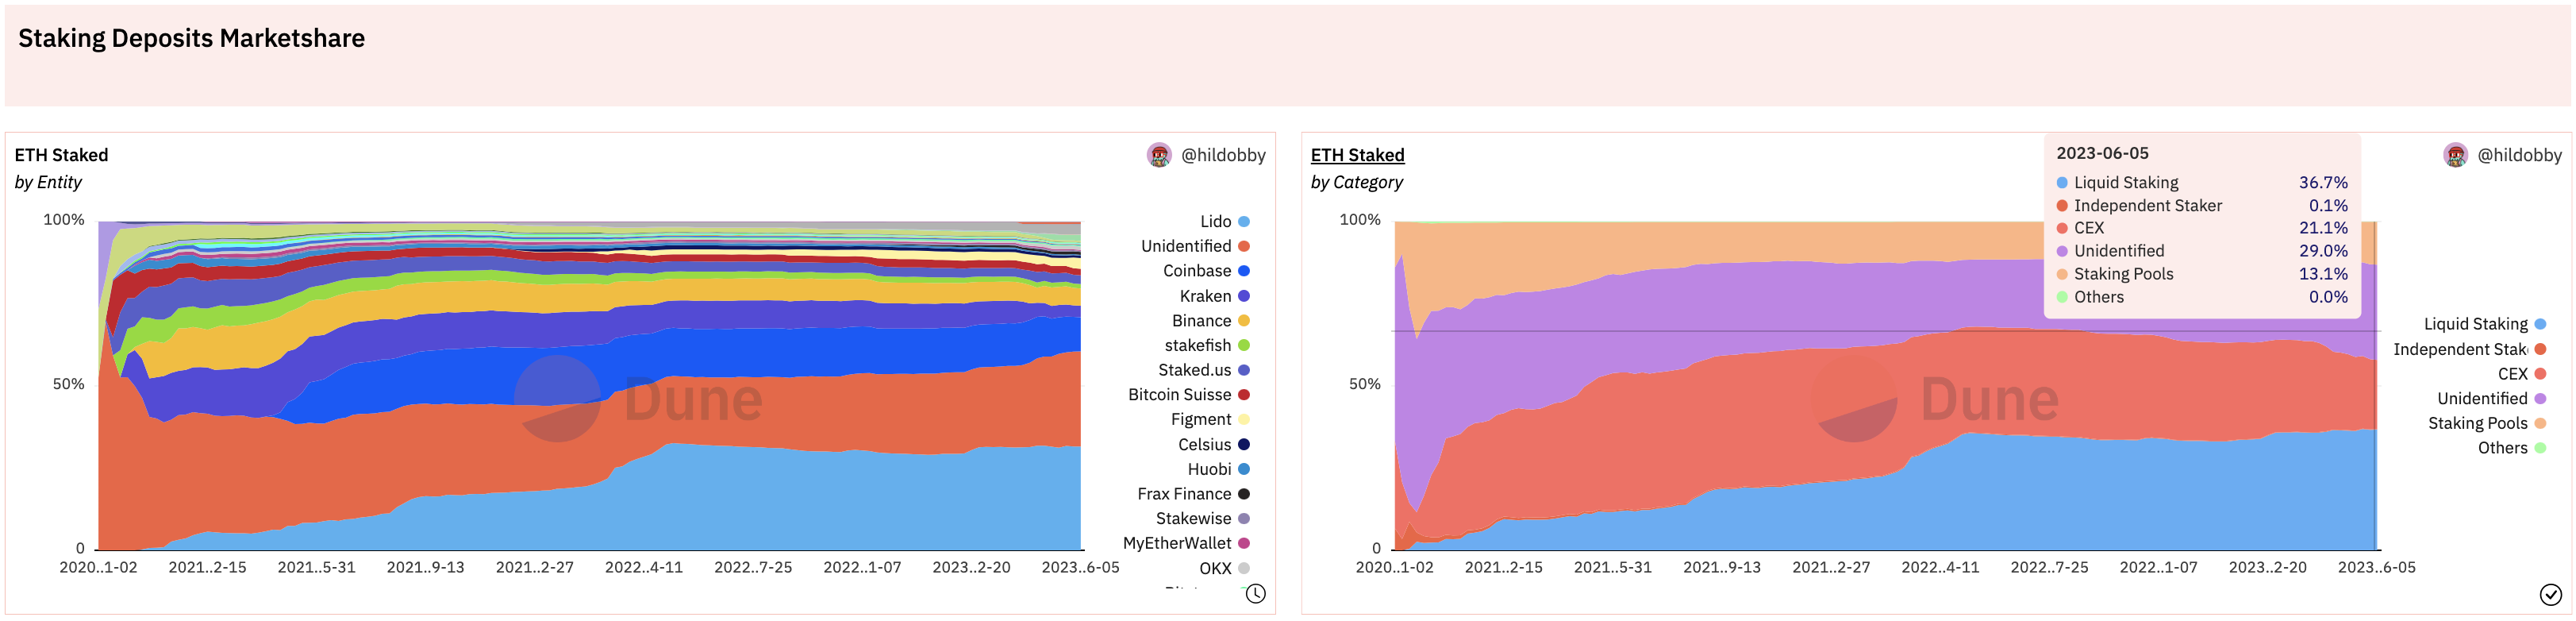
\includegraphics[width=\linewidth]{../images/hildobby10}
%\caption{Dune Analytics Staking deposit market share. @hildobby  (7 June 2023)}
%\label{fig:hildobby=10}
%\end{center}
%\end{figure}
%
%\begin{figure}[htbp]
%\begin{center}
%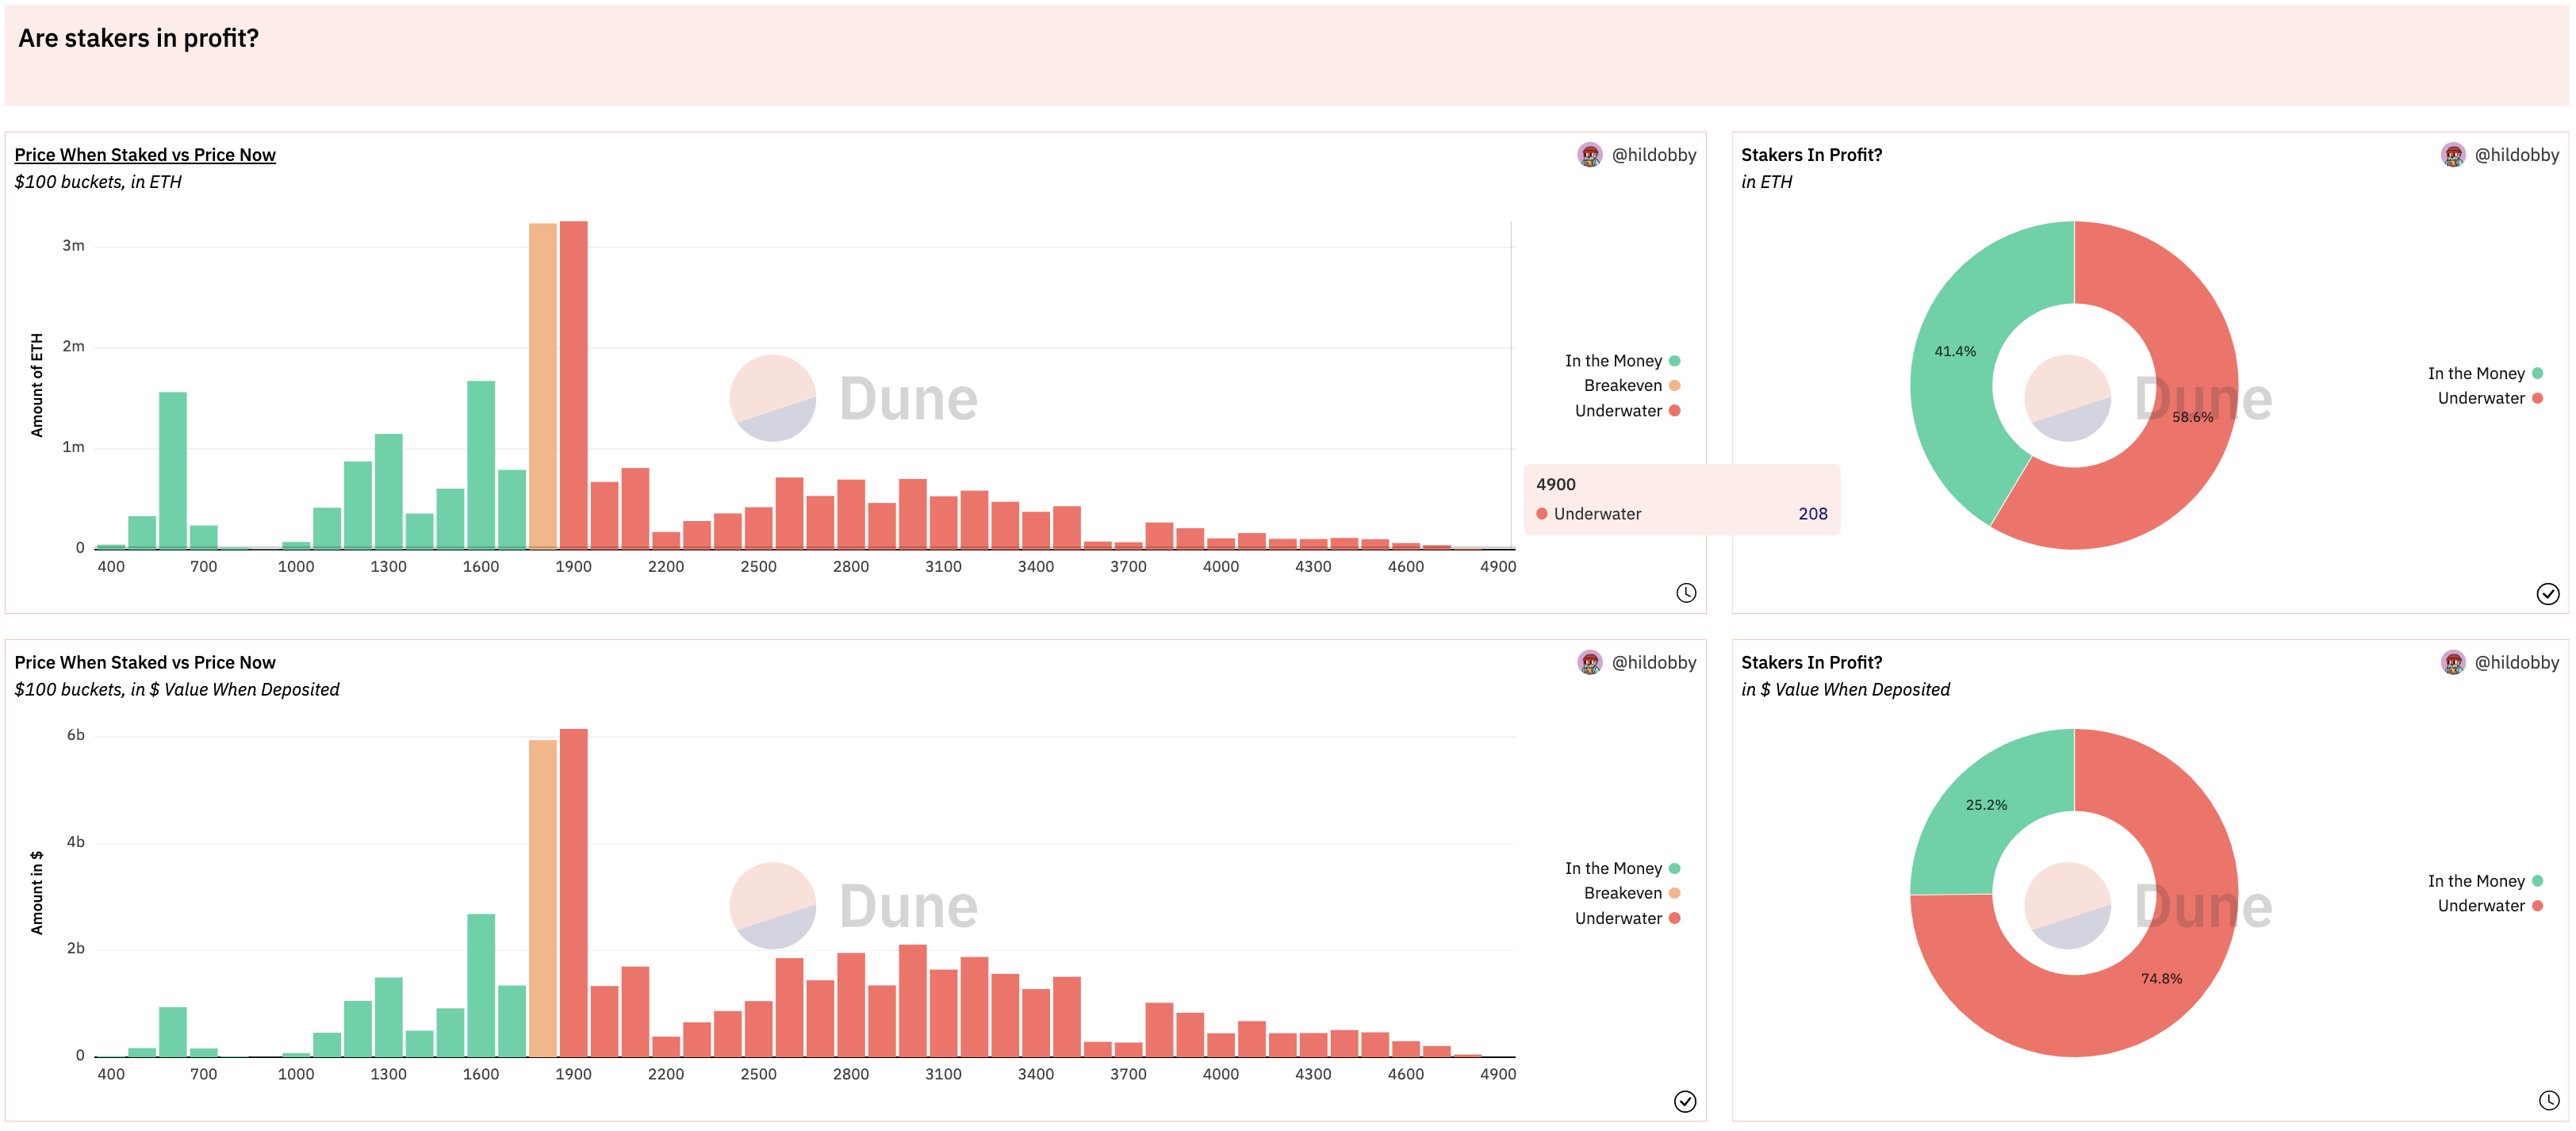
\includegraphics[width=\linewidth]{../images/hildobby11}
%\caption{Dune Analytics Staker profit. @hildobby  (7 June 2023)}
%\label{fig:hildobby=11}
%\end{center}
%\end{figure}
%
%\clearpage

% =================
\section{Validators}
% ===================
\label{sec:validators}
% ---------------------------------------------------------------
\subsection{Validator slashing and penalties}
% ---------------------------------------------------------------
\label{slashing} \subsubsection*{Slashing} The situations that lead to a
validator being slashed are few, but they are severe violations of protocol
rules that may be considered as a potential solo or coordinated attack on the
system. Regardless of the reason for the slashing event, they are all handled
in the same way. There is an initial slashing penalty, which is currently set
at 1 ETH (or $\frac{1}{32}$ of the stake) and this is followed 18 days after
the slashing event by another penalty, known as the correlation penalty. The
purpose of the latter is to penalise what may be a coordinated attack on the
chain. Therefore the correlation penalty takes into account slashings 18 days
before and after the slashing event. 

A validator gets slashed when they are reported and evidence of the violation
of the rules is included in a beacon block. For the valid reporting of a
slashing event, the reporting validator receives a reward. The intention is
that this will help incentivise the reporting of slashable events. Only one
proposer slashing can be included in a report, whereas multiple attestation
violations can be included in a report. When the slashing is included in a
block, the proposer gets a reward which is a fraction of the effective balance
of the validator being slashed (currently $\frac{1}{512}$). Up to 16 proposer
slashings can be included in a block and up to 2 attester slashing reports. 
Therefore, if several slashings have occurred, including these reports in a
block can generate a generous reward for the proposer. 

For more detailed information on slashing and calculations, please refer to the 
latest version of Edgington's
\href{https://eth2book.info/capella/part2/incentives/slashing/}{\textit{Upgrading Ethereum}}
book \cite{Edgington2023}  which incorporates the updates included in the 
Capella hard fork. In summary the events that lead to slashing are:

\begin{enumerate}
  \item ``making two differing attestations for the same target checkpoint''
  \item ``making an attestation whose source and target votes `surround' those
    in another attestation from the same validator.
  \item ``proposing more than one distinct block at the same height''
  \item ``attesting to different head blocks, with the same source and target
    checkpoints''
\end{enumerate}

The first two relate to Casper \gls{ffg} consensus, and the latter two are
related to \gls{lmd} \gls{ghost} consensus.

Edgington points out that `slashable behaviours relate to ``equivocation'',
which is when a validator contradicts something it previously advertised to the
network'. Hence it is important for validators to ensure that they do not
`accidentally' equivocate. This could theoretically happen as a result of bugs
in client software, but the vast majority of slashings have been due to node
operators running two different nodes using the same validator keys. The reason
may have been to improve uptime, but the risk of slashing is too great compared
to any potential benefit in uptime \cite{Edgington2023}. There was also an
incident where a validator exploited a vulnerability in a relay operator
running mev-boost, an open source proposer-builder separation protocol.
Flashbots posted a 
\href{https://collective.flashbots.net/t/post-mortem-april-3rd-2023-mev-boost-relay-incident-and-related-timing-issue/1540}{detailed post-mortem of the event}.

Apart from the slashing penalties, a slashed validator accrues attestation
penalties until such time as they exit, which is not until $2^{13} \texttt{
}epochs = 8,192 \texttt{ }epochs \approx 36 \texttt{ } days$ after being
slashed. Moreover,  if there is an inactivity leak at the time, the penalties
imposed on slashed validators will be higher. Slashed validators cannot earn
any attestation rewards while waiting to exit. It seems rather odd, but a
slashed validator can still be elected to be the proposer for the next block.
However, their block will be deemed to be invalid. The only duty for which they
could receive a small reward is if they are selected to be in the sync
committee, but the probability of this happening is very small. 

\subsubsection*{Penalties} Slashing is the most severe penalty a validator is
subjected to and as explained they can accrue several extra penalties while
they wait to exit. However, there are a number of smaller, less serious
`misdemeanours', or failure to perform their duties that can result in
penalties for validators. The validator's stake is reduced by the penalty and
the ETH is burnt, thereby reducing net issuance \cite{Edgington2023}. \\

\textit{Attestation penalties}
\begin{itemize}
  \item Missed source and target votes (i.e. missed Casper FFG votes), but no
    penalty for a missed head vote.
  \item Incorrect source vote, then target vote is missed.
  \item Incorrect source or target vote, then head vote is missed.
\end{itemize}

\textit{Sync committee penalties}
\begin{itemize}
  \item Non-participation of a member incurs a penalty equivalent to the reward
    they would have received if it was correct
\end{itemize}

%\subsection{Data sources \& visualisations}
%% -----------------------------------------------------------
%\label{sec:data}
%\subsubsection*{Data from an archive node}
%% --------------------------------------------------------
%Accessing a teku-besu archive node, \texttt{teku-besu-ohio-mainnet-archive-01},  we were able to use several API endpints to extract some rich data for validators.\\
%	 We selected several API endpoints from those listed in GitHub: \href{https://ethereum.github.io/beacon-APIs/?urls.primaryName=dev}{Eth Beacon Node API}\\
%	 Some visualisations of validator information from the archive node are in figures~\ref{fig:dailyvalidator1}~-~\ref{fig:cumulativevalidatorsregression}, pages~\pageref{fig:dailyvalidator1}~-~\pageref{fig:cumulativevalidatorsregression}.
%
%\clearpage
%\textbf{Graphs of validator data}
%% -------------------------------------------
% \begin{figure}[htbp]
%\begin{center}
%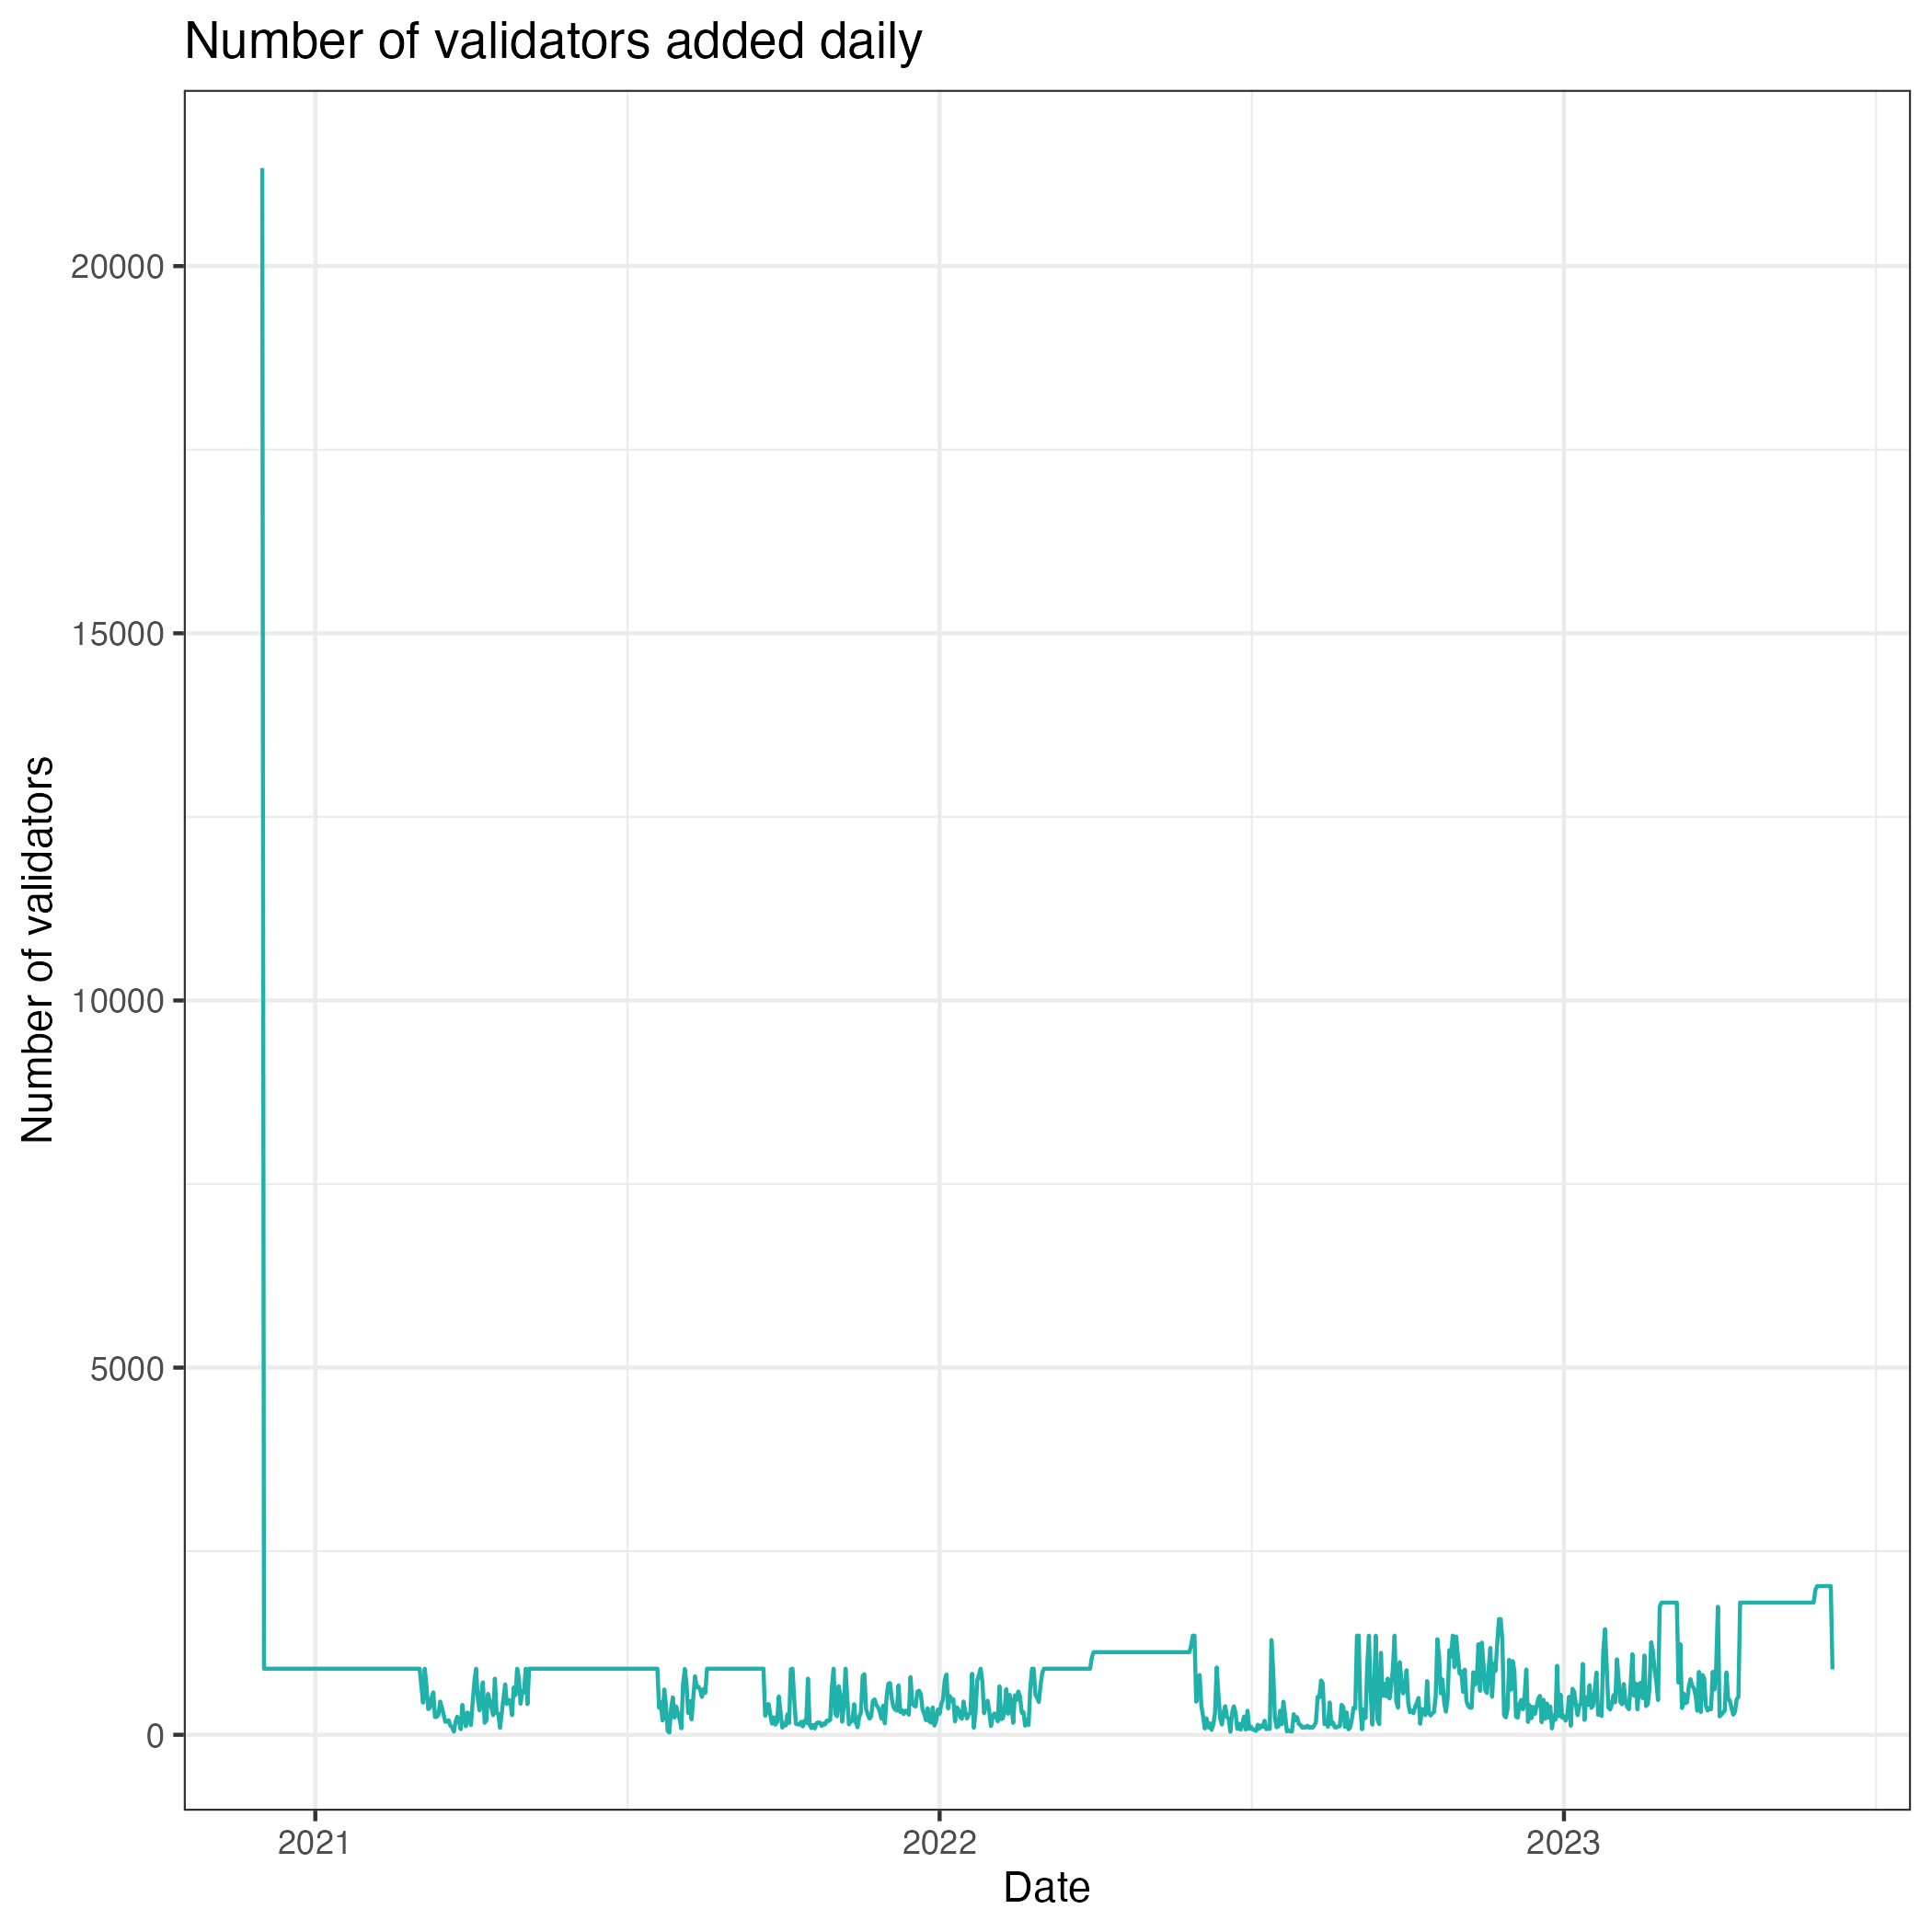
\includegraphics[width=\linewidth]{../images/daily_validator_plot_230607}             % Note: Within images, no need to use \_ for _
%\caption{Number of validators added daily}
%\label{fig:dailyvalidator1}
%\end{center}
%\end{figure} 
%
%\begin{figure}[htbp]
%\begin{center}
%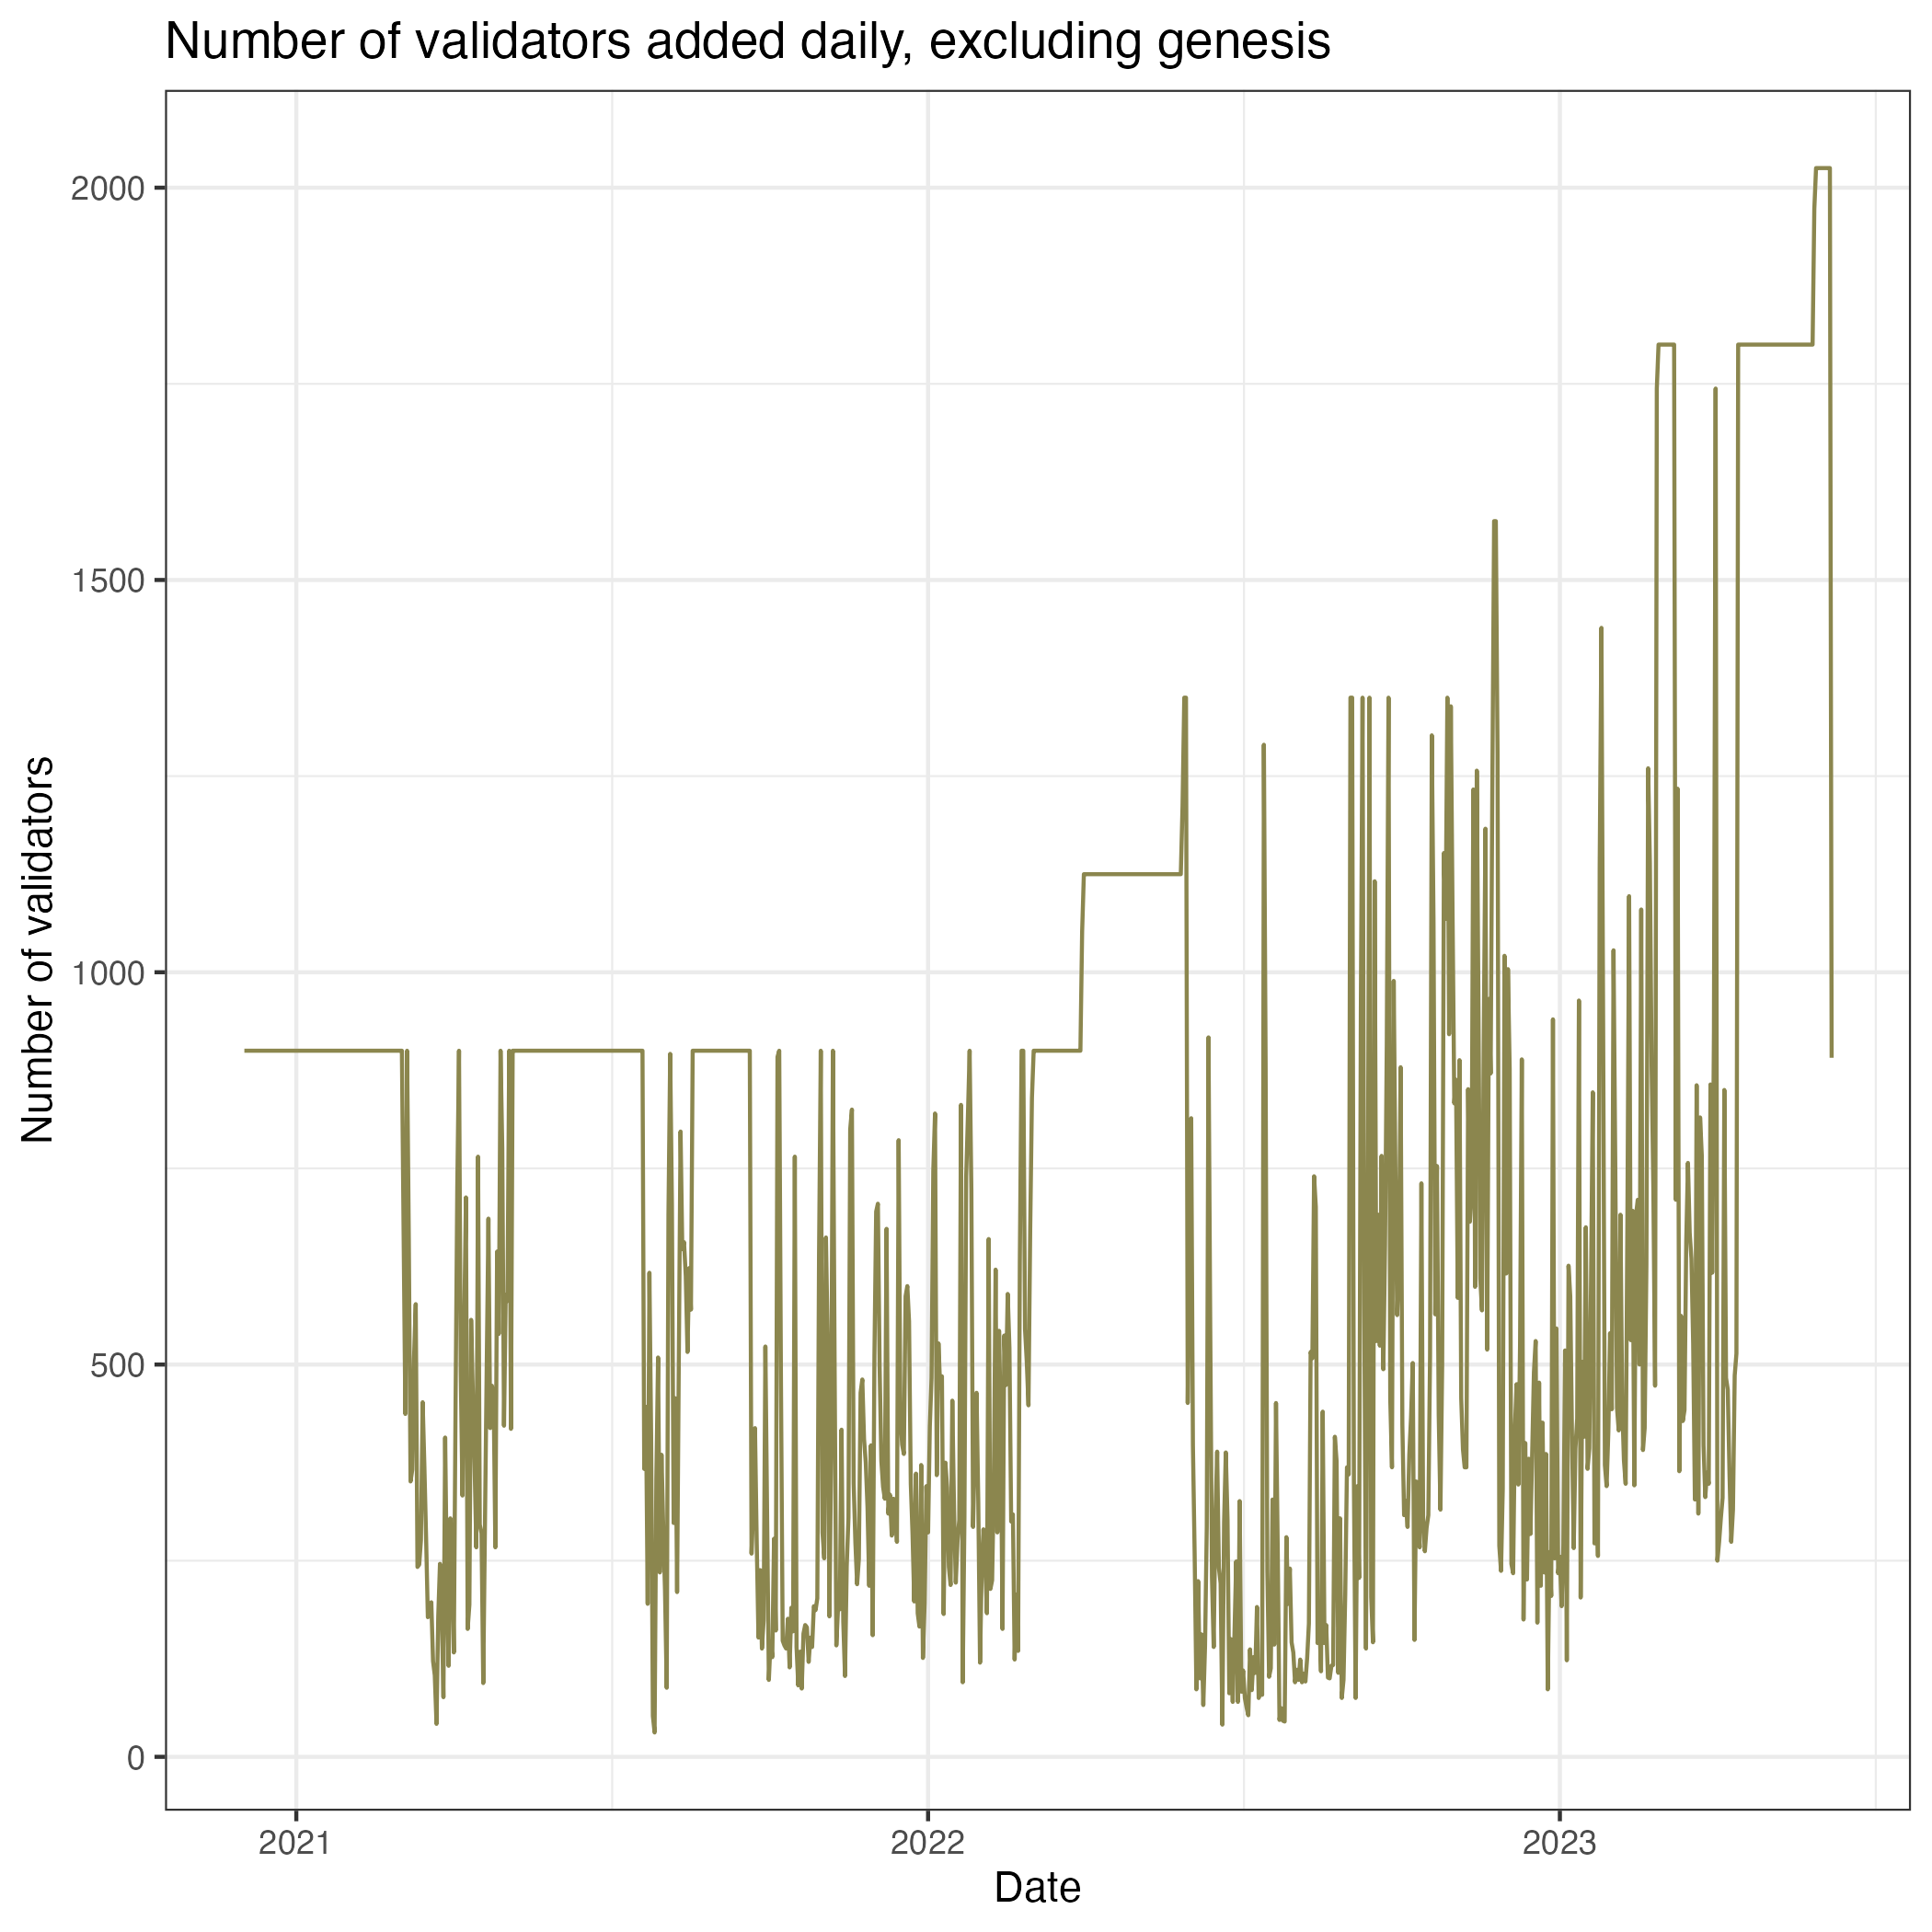
\includegraphics[width=\linewidth]{../images/daily_validator_plot_no_genesis_no_smoothing_230607}             % Note: Within images, no need to use \_ for _
%\caption{Number of validators added daily, excluding genesis}
%\label{fig:dailyvalidator2}
%\end{center}
%\end{figure}
%
%\begin{figure}[htbp]
%\begin{center}
%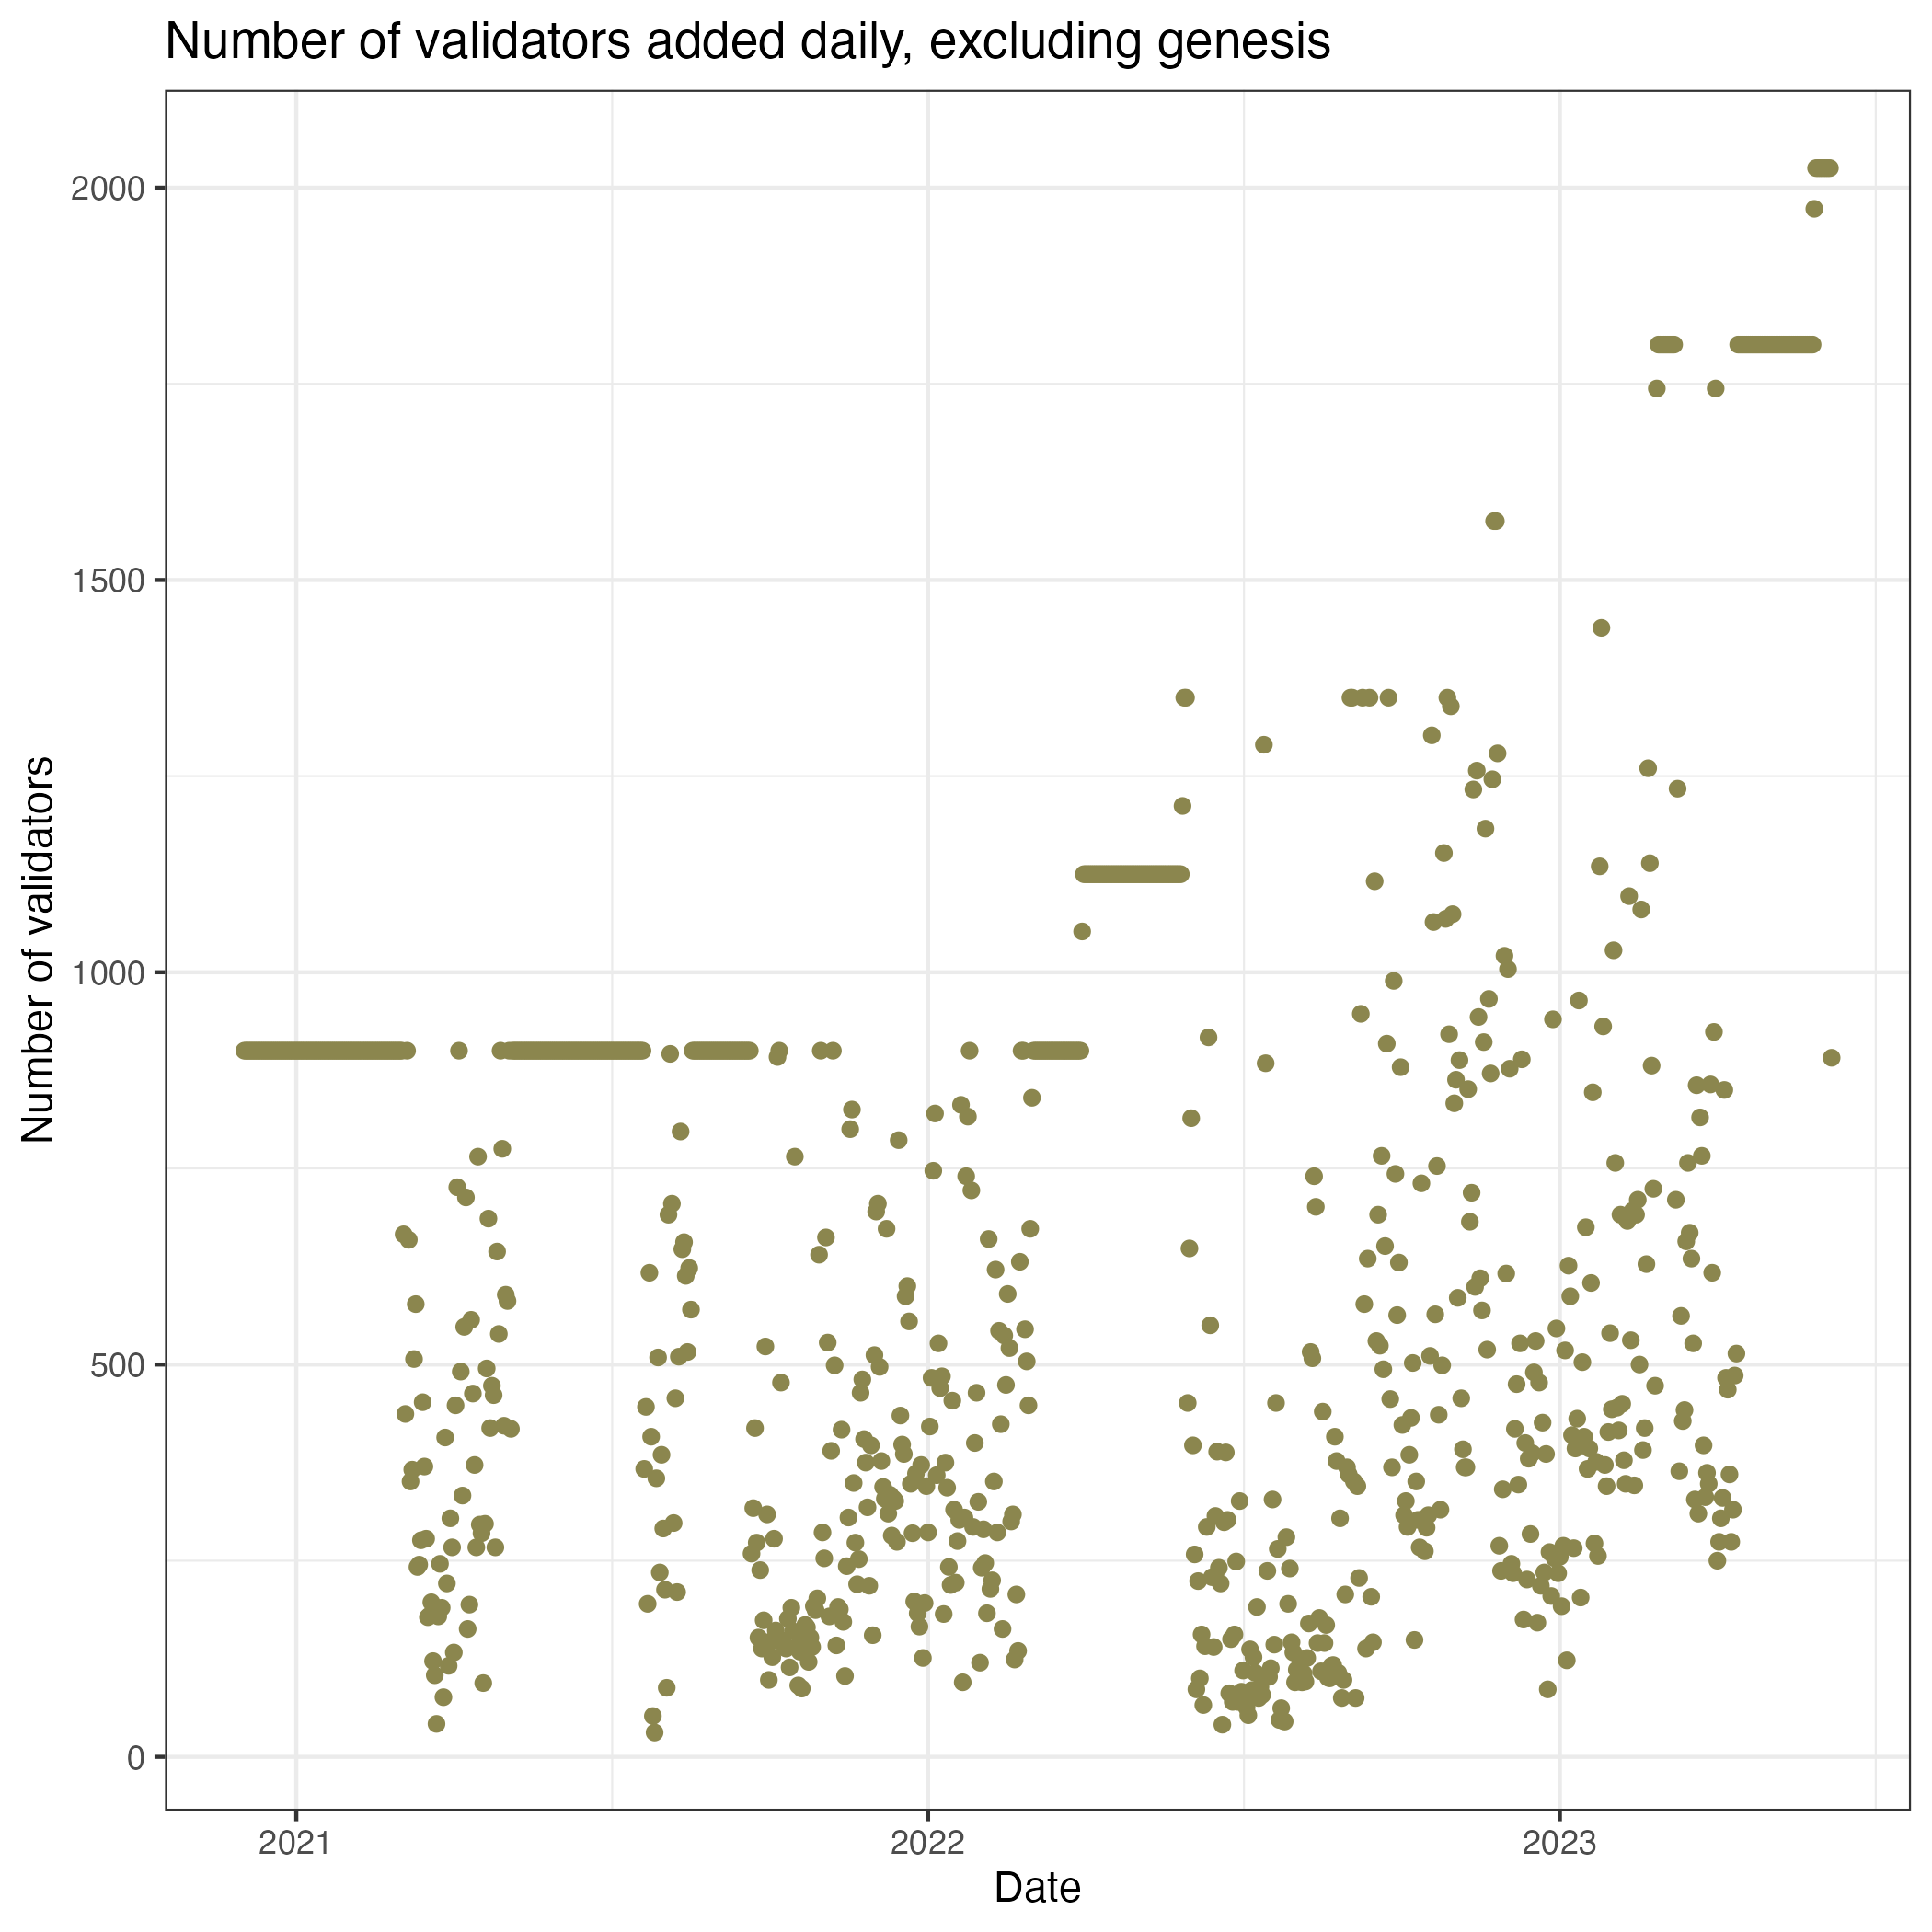
\includegraphics[width=\linewidth]{../images/daily_validator_plot_no_genesis_pt_no_smoothing_230607}             % Note: Within images, no need to use \_ for _
%\caption{Number of validators added daily, excluding genesis}
%\label{fig:dailyvalidator3}
%\end{center}
%\end{figure}
%
%\begin{figure}[htbp]
%\begin{center}
%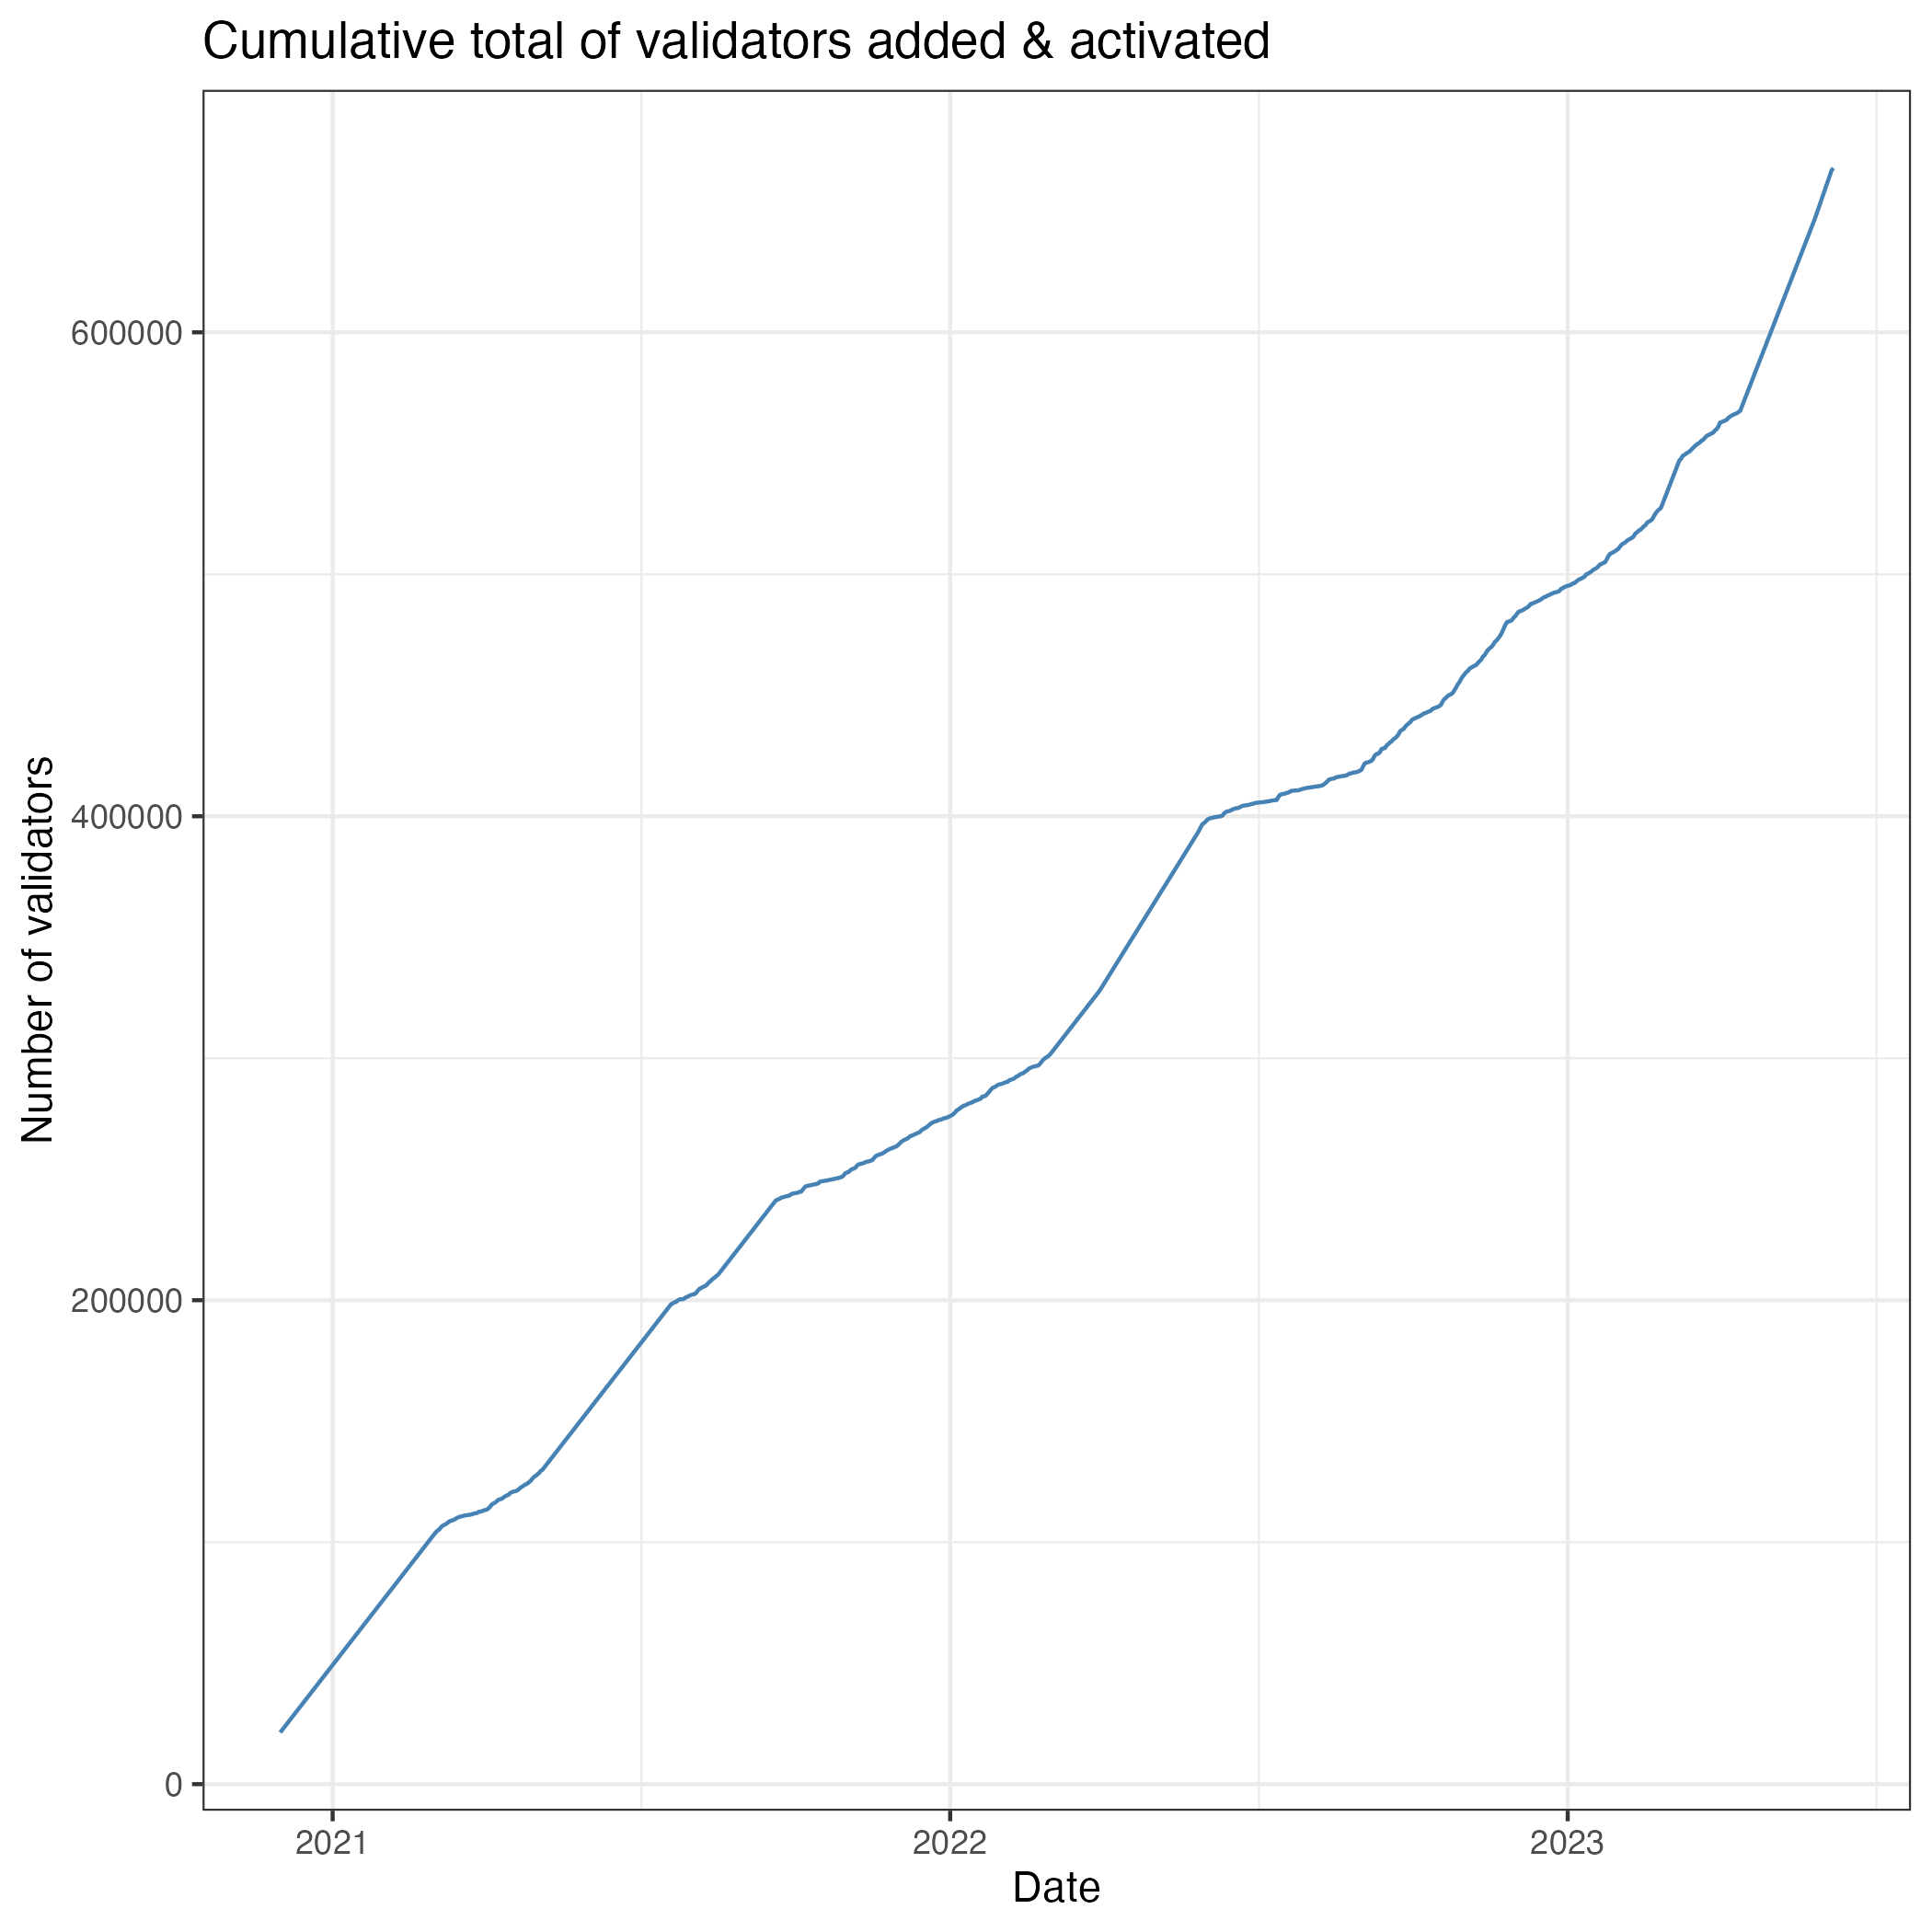
\includegraphics[width=\linewidth]{../images/cumulative_validator_plot_230607}
%\caption{Cumulative total of validators added \& activated}
%\label{fig:cumulativevalidators}
%\end{center}
%\end{figure}
%
%
% \begin{figure}[htbp]
%\begin{center}
%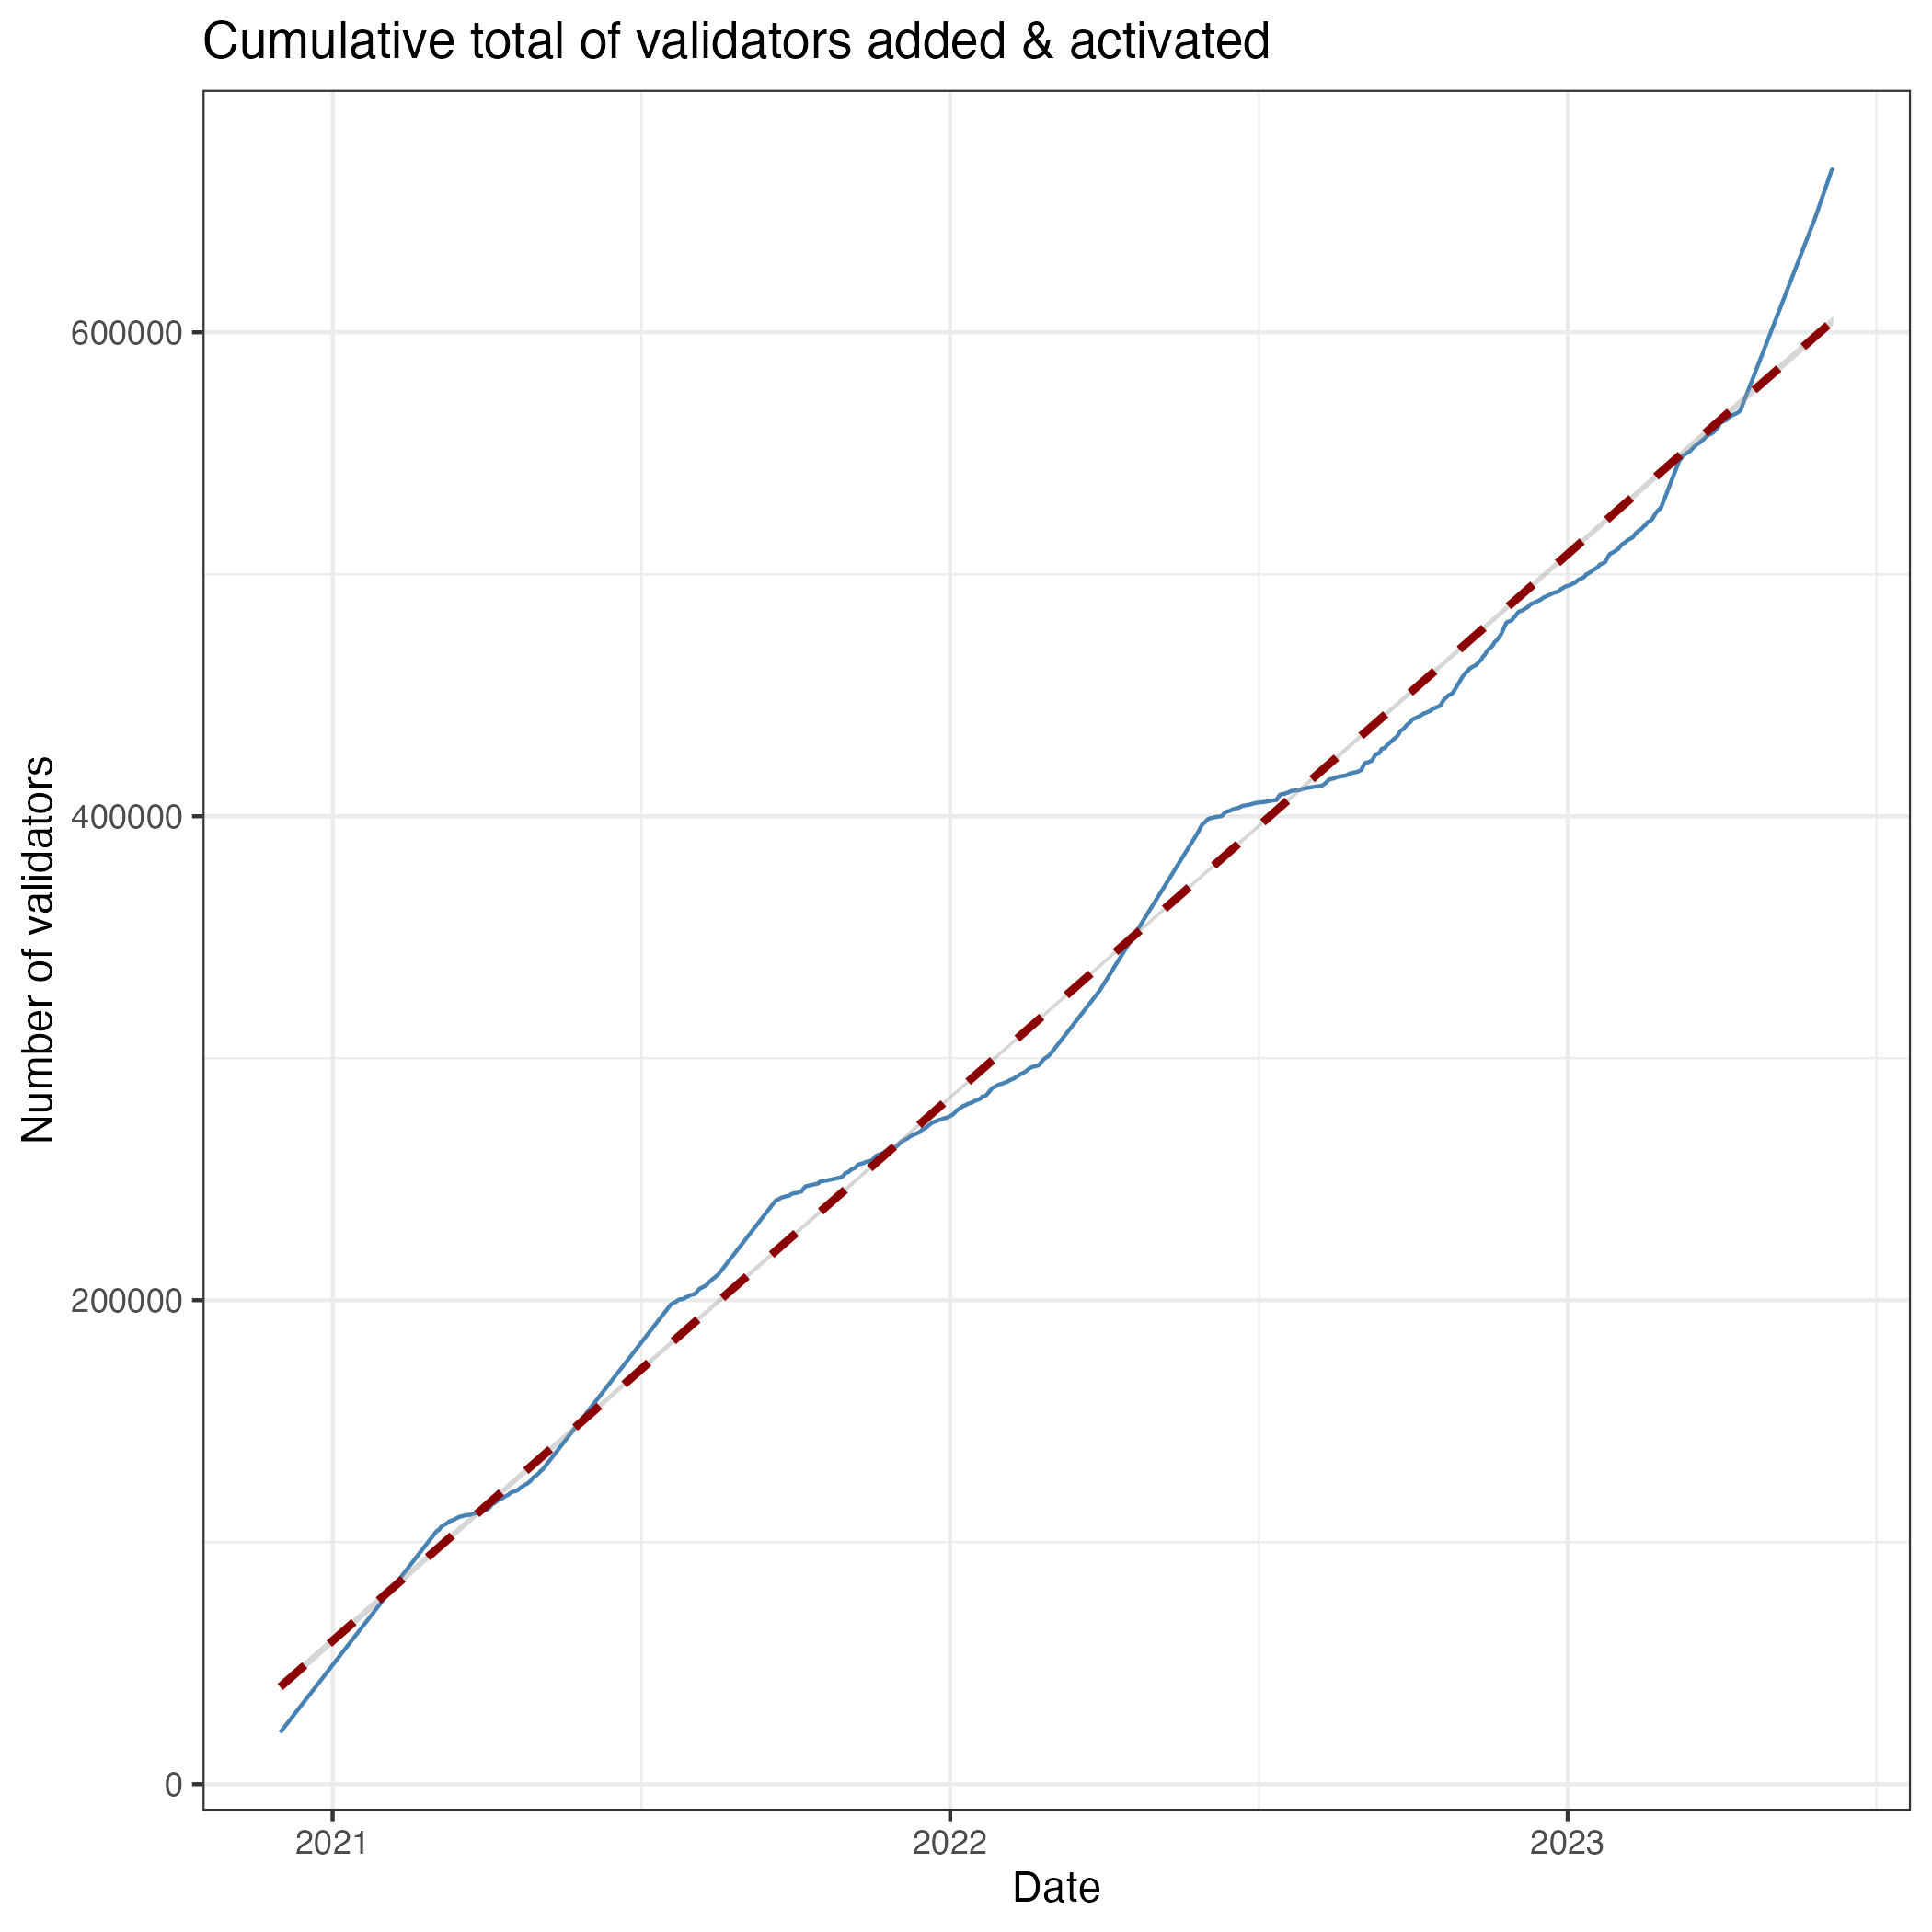
\includegraphics[width=\linewidth]{../images/cumulative_validator_plot_with_regression_line_230607}
%\caption{Cumulative total of validators added \& activated with regression line fitted}
%\label{fig:cumulativevalidatorsregression}
%\end{center}
%\end{figure}
%
%\clearpage	 
%% --------------------------------------
%\subsubsection*{Rated network explorer}
%% --------------------------------------
%\textbf{Entity Views} \\
%% ----------------------------------
%\begin{figure}[htbp]
%\begin{center}
%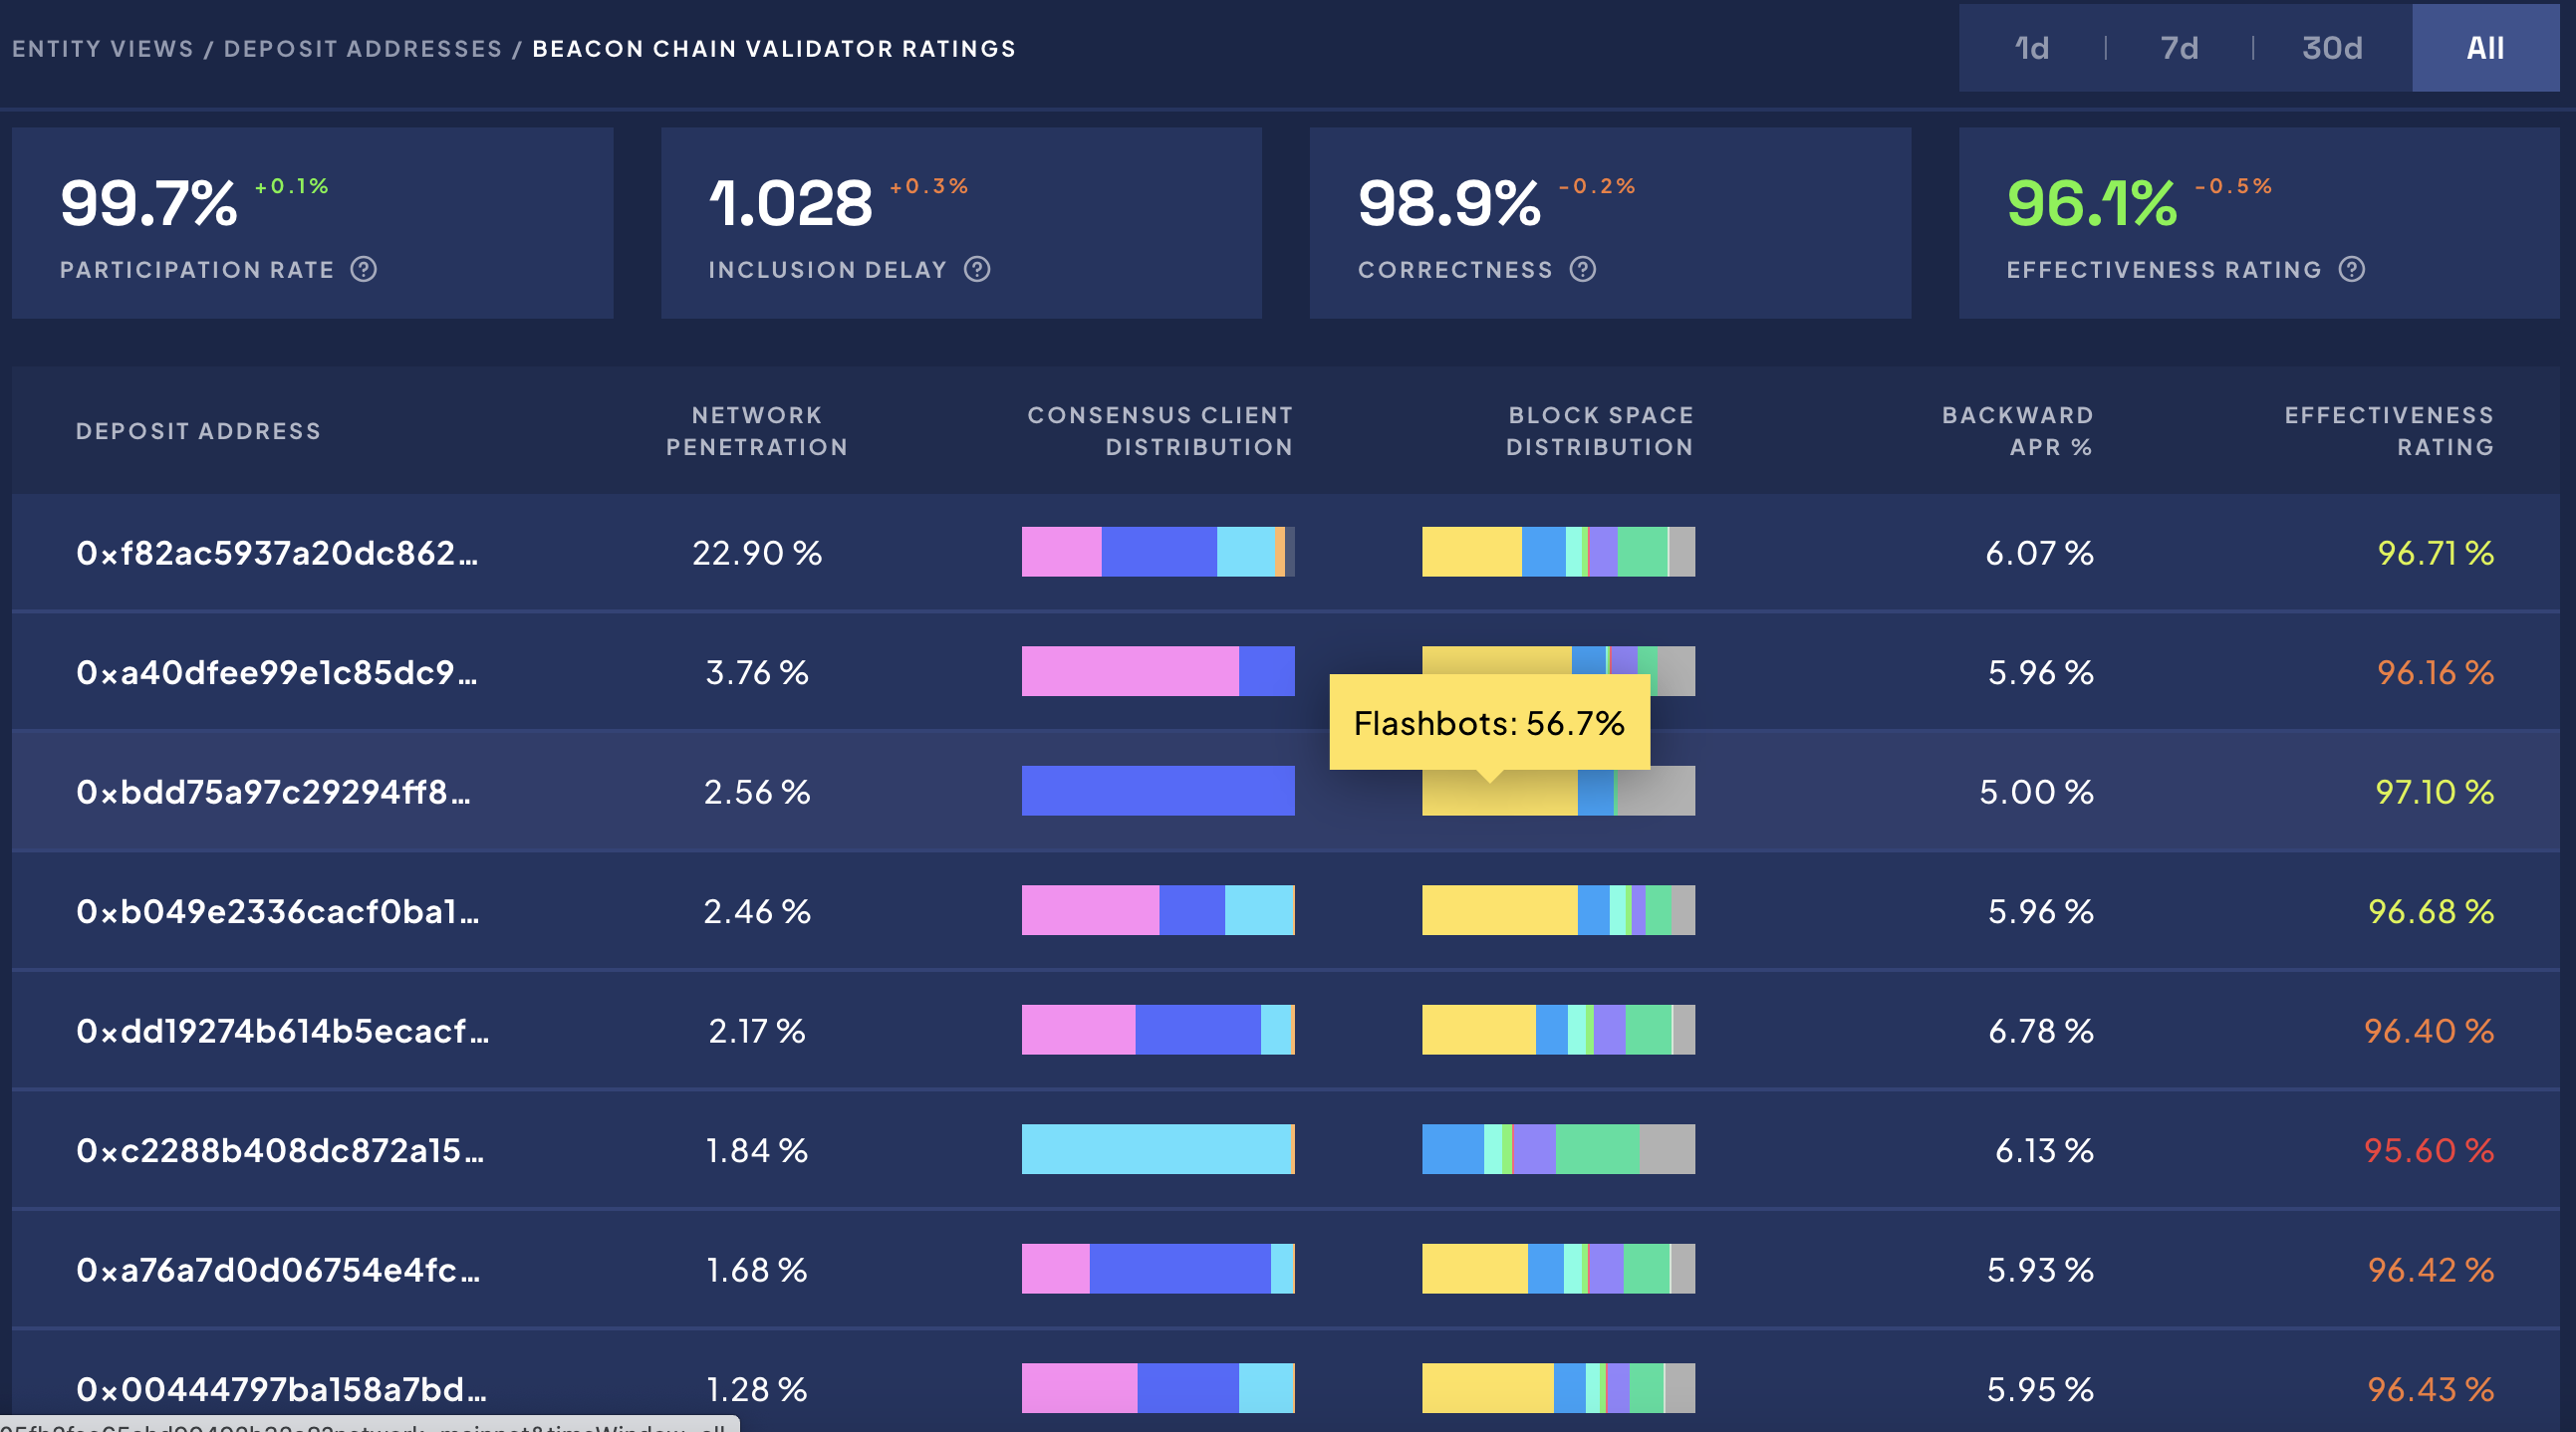
\includegraphics[width=\linewidth]{../images/ratedentity3}
%\caption{Rated network explorer: beacon chain validator ratings by deposit addresses. Select from timeframes: 1 day, 7 days, 30 days, or all (since merge) , 1 June 2023}
%\label{fig:ratedentity3}
%\end{center}
%\end{figure}
%
%\begin{figure}[htbp]
%\begin{center}
%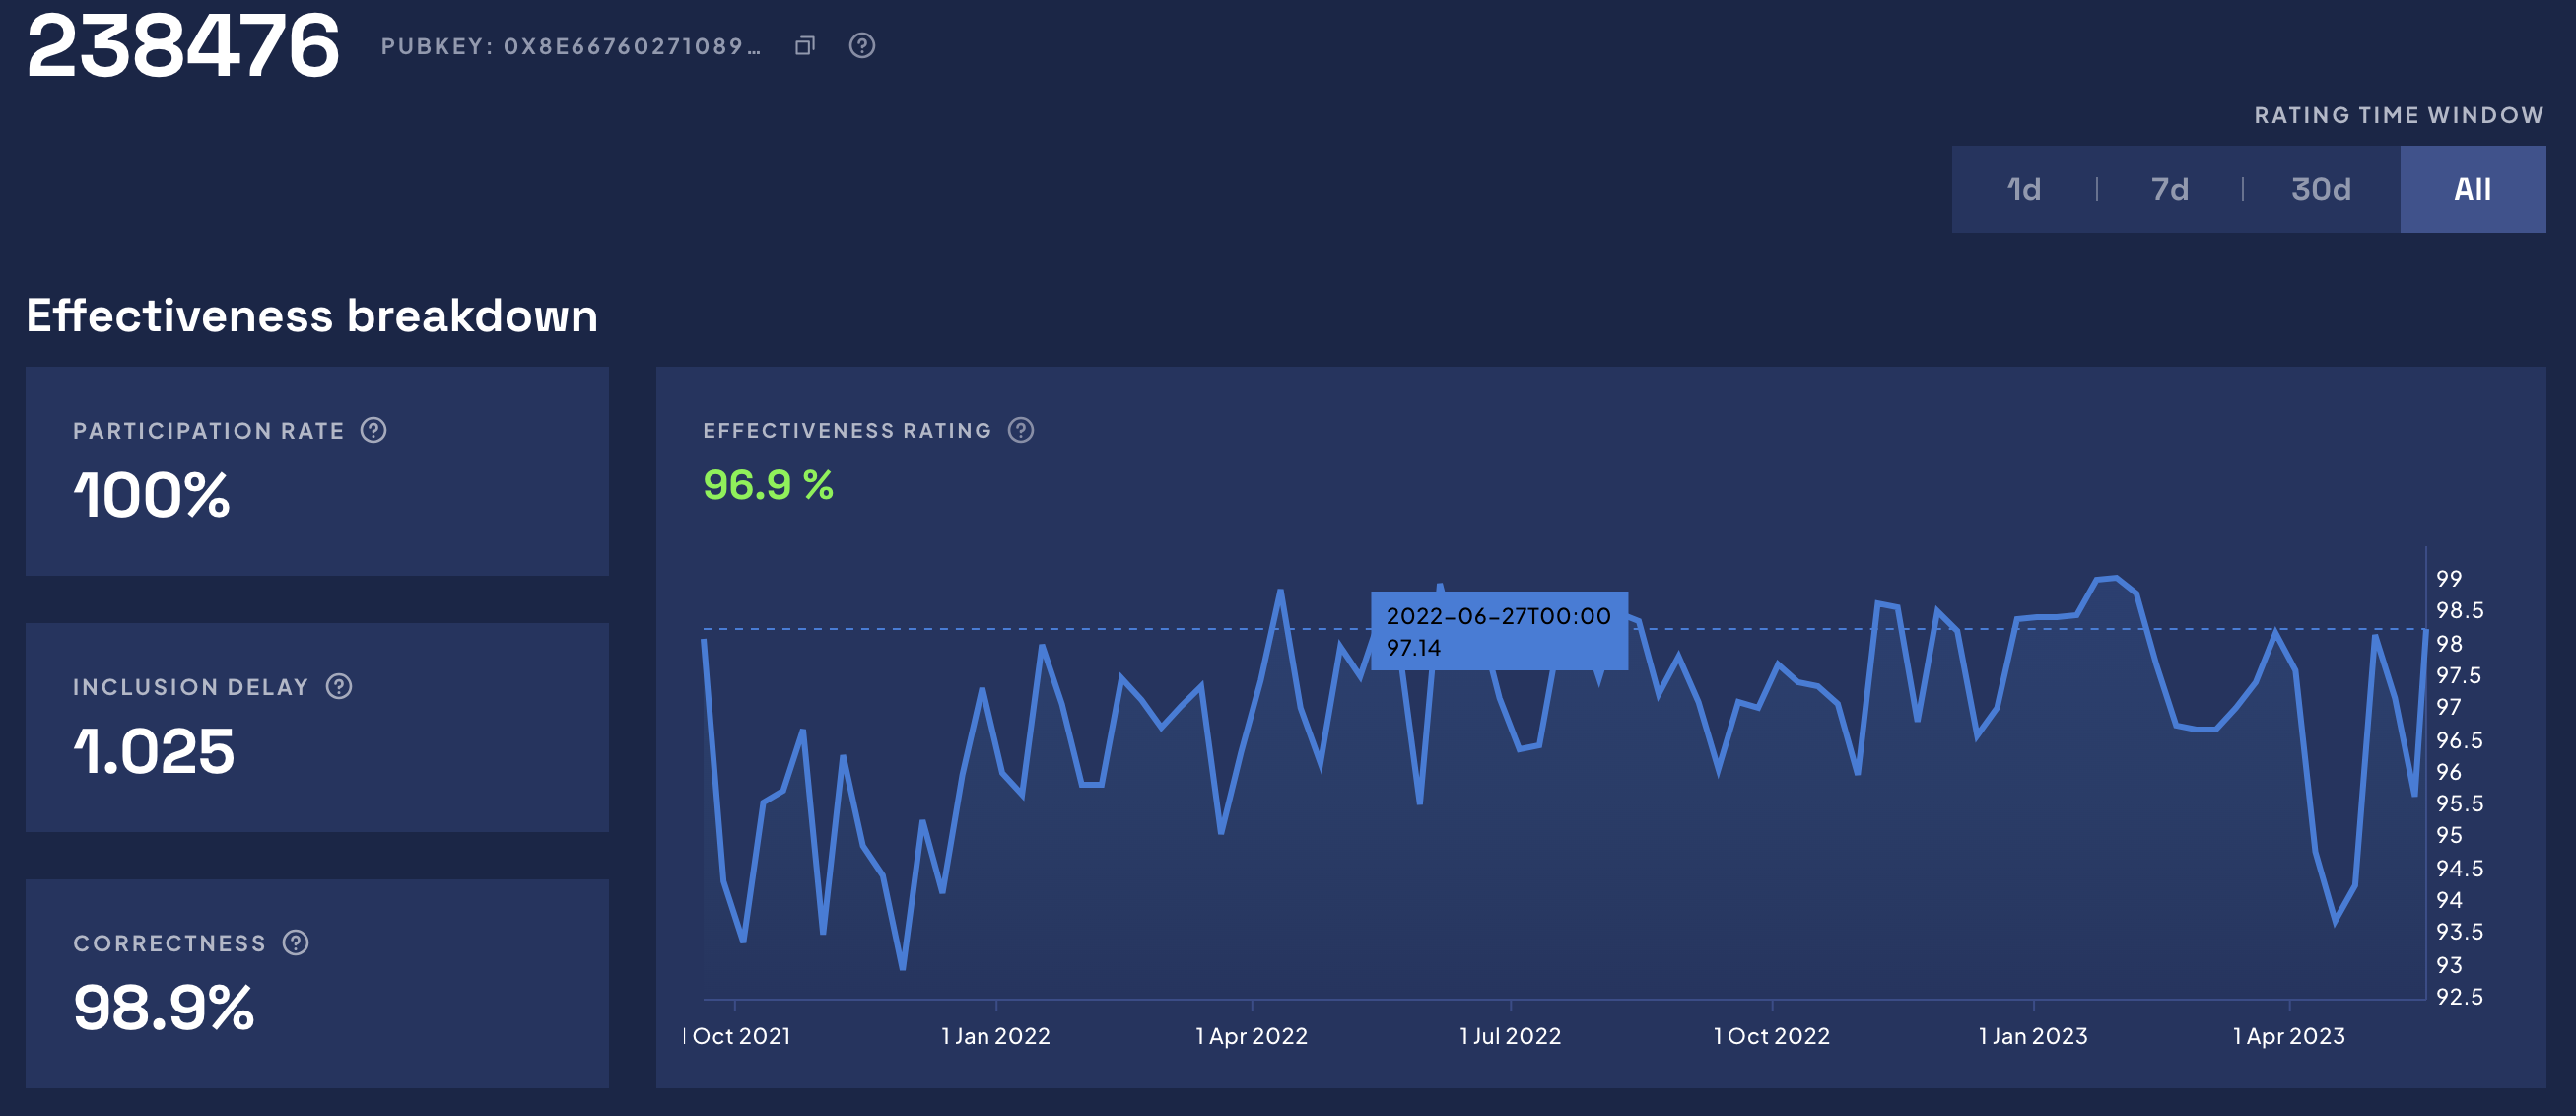
\includegraphics[width=\linewidth]{../images/ratedentity4a}\\
%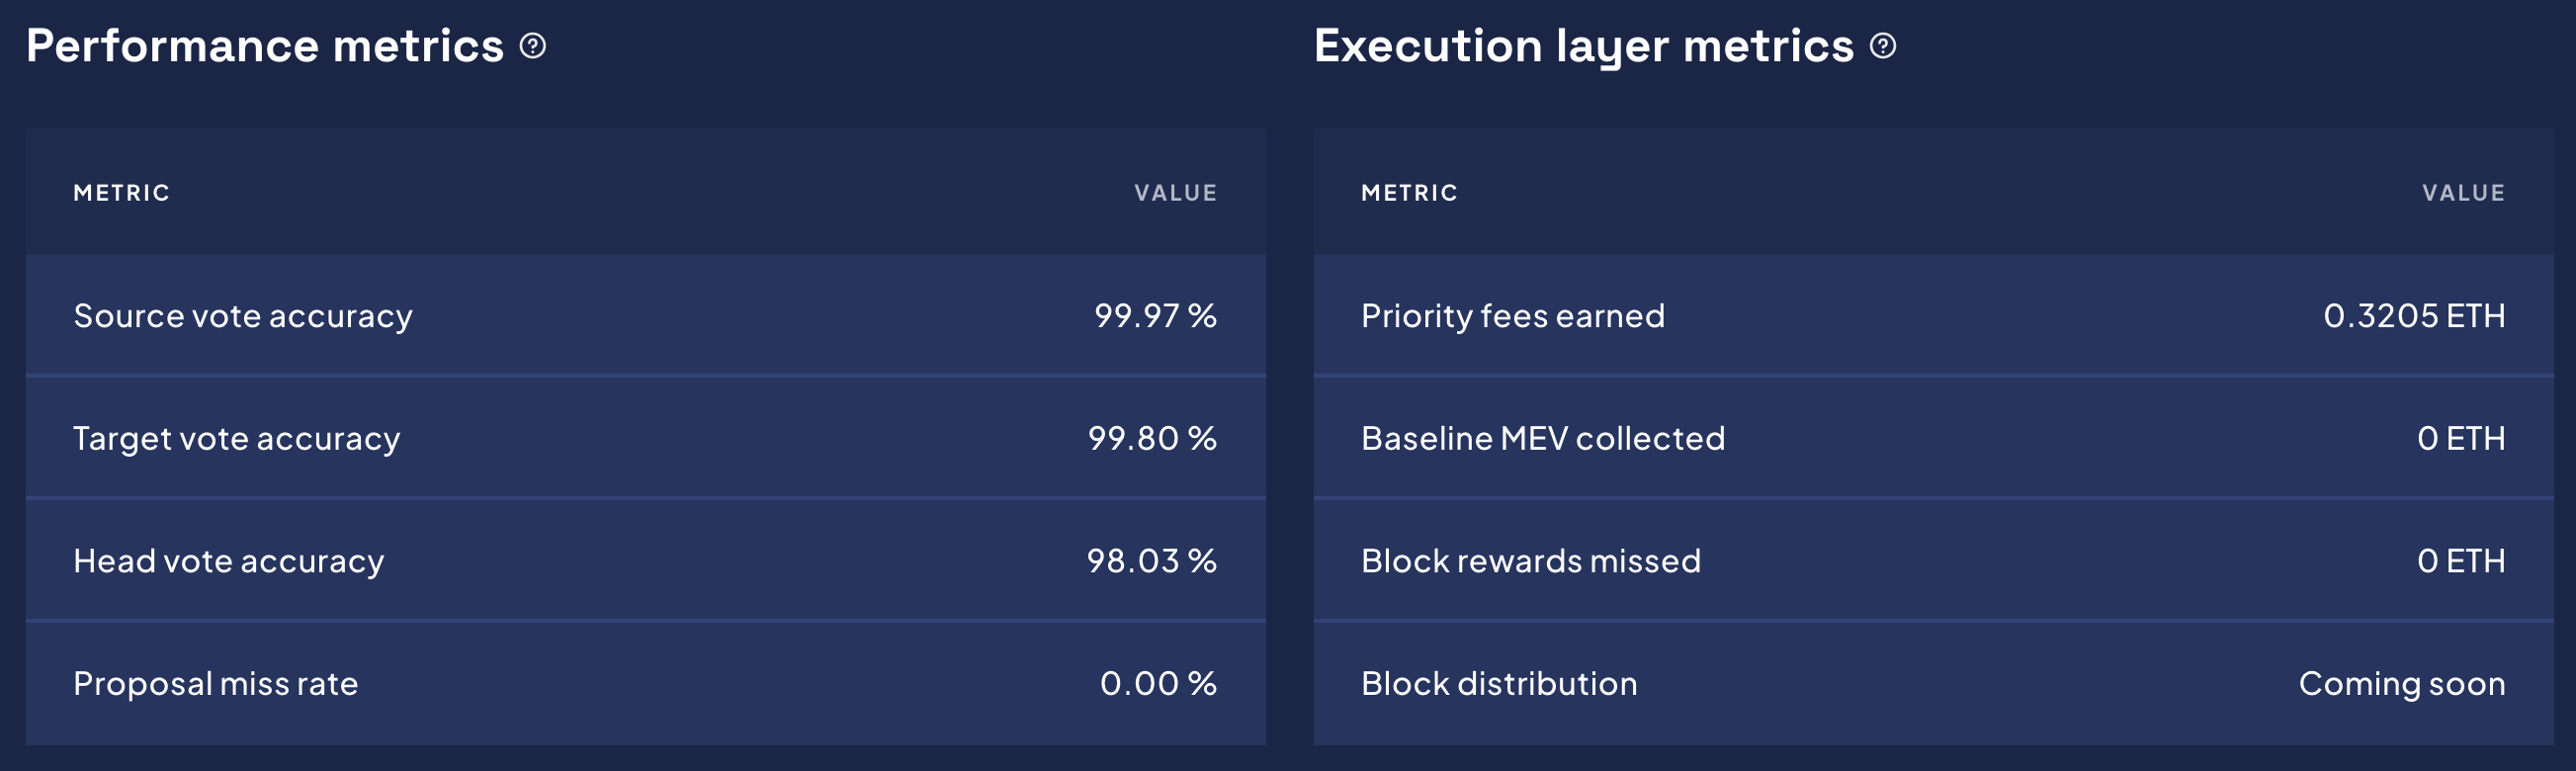
\includegraphics[width=\linewidth]{../images/ratedentity4b}\\
%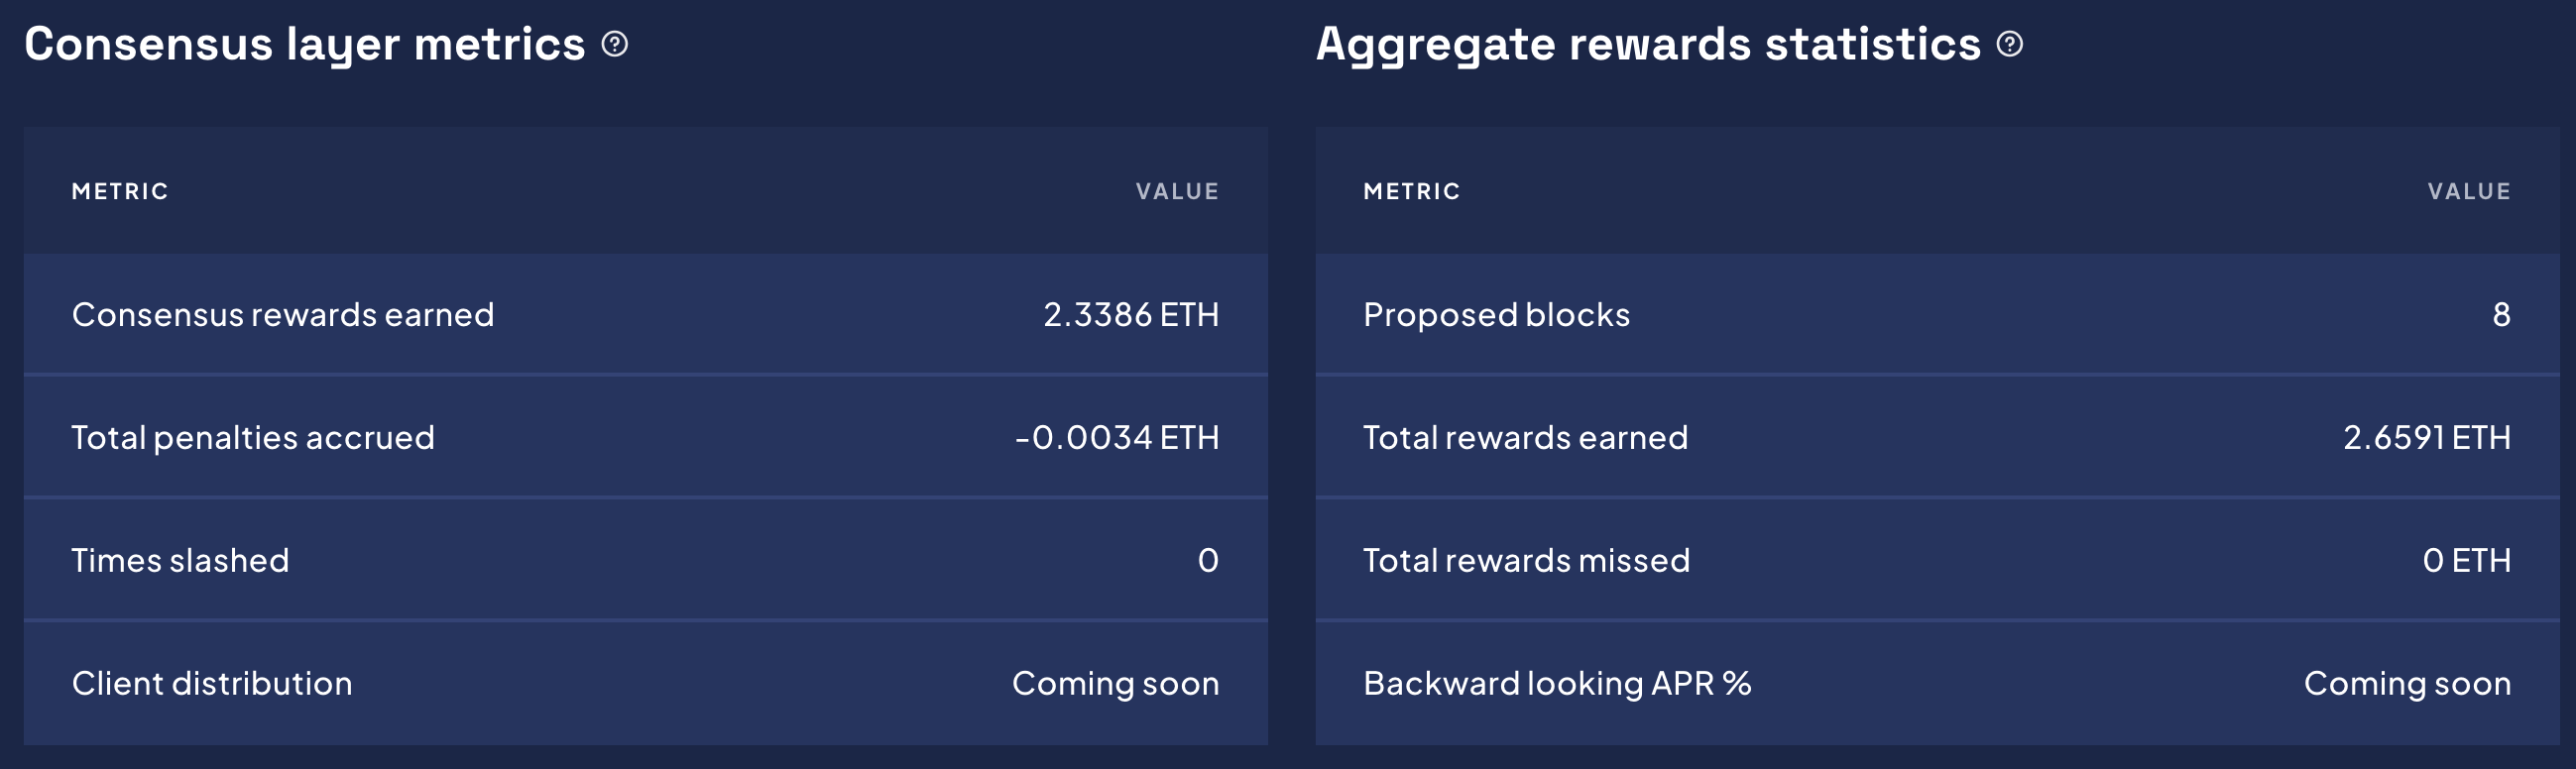
\includegraphics[width=\linewidth]{../images/ratedentity4c}
%\caption{Rated network explorer: view of a chosen validator (using id or public key). Select from timeframes: 1 day, 7 days, 30 days, or all (since merge) , 1 June 2023}
%\label{fig:ratedentity4}
%\end{center}
%\end{figure}
%
%\textbf{Aggregate Views} 
%% ----------------------------------
%
%\begin{figure}[htbp]
%\begin{center}
%\includegraphics[width=\linewidth]{../images/ratednw1}\\
%(a)
%\includegraphics[width=\linewidth]{../images/ratednw2}\\
%(b)
%\caption{Rated network explorer: high level metrics to reflect the health of the network  (a) and four reference rates of return for the entire active validator set. (b), For both visualisations, select a timeframe: 1 day, 7 days, 30 days or all (since merge),1 June 2023}
%\label{fig:ratednw1}
%\end{center}
%\end{figure}
%
%\begin{figure}[htbp]
%\begin{center}
%\includegraphics[width=\linewidth]{../images/ratednw3}\\
%(a)
%\includegraphics[width=\linewidth]{../images/ratednw4}\\
%(b)
%\caption{Rated network explorer: activation \& exits information: the number of validators activated and the proportion of activation capacity for selected timeframe, and similarly for validators exiting.  (a) and four reference rates of return for the entire active validator set. (b), For both visualisations, select a timeframe: 1 day, 7 days, 30 days or all (since merge),1 June 2023}
%\label{fig:ratednw4}
%\end{center}
%\end{figure}
%
%\textbf{MEV Relay Landscape}\\
%% ---------------------------------------
%\begin{figure}[htbp]
%\begin{center}
%\includegraphics[width=\linewidth]{../images/ratedrelay1}
%\caption{Rated network explorer: MEV relay summary statistics for 30 days, selected from timeframes: 1 day, 7 days, 30 days or all (since merge), 6 June 2023}
%\label{fig:ratedrelay1}
%\end{center}
%\end{figure}
%
%\begin{figure}[htbp]
%\begin{center}
%\includegraphics[width=\linewidth]{../images/ratedrelay2}
%\caption{Rated network explorer: Comparison between MEV relays for blocks procured from relays that were included in the canonical chain for all days, selected from timeframes: 1 day, 7 days, 30 days or all (since merge), 6 June 2023}
%\label{fig:ratedrelay2}
%\end{center}
%\end{figure}
%
%\begin{figure}[htbp]
%\begin{center}
%\includegraphics[width=\linewidth]{../images/ratedrelay3}
%\caption{Rated network explorer: MEV-boost relay market share selecting all days from timeframes: 1 day, 7 days, 30 days or all (since merge), 6 June 2023}
%\label{fig:ratedrelay3}
%\end{center}
%\end{figure}
%
%\clearpage
%\textbf{MEV Builder Landscape}
%% ---------------------------------------
%\begin{figure}[htbp]
%\begin{center}
%\includegraphics[width=\linewidth]{../images/ratedbuilder}
%\caption{Rated network explorer: MEV relay summary statistics for 30 days, selected from timeframes: 1 day, 7 days, 30 days or all (since merge), 6 June 2023}
%\label{fig:ratedbuilder}
%\end{center}
%\end{figure}
%

% ---------------------------------------------------------------
\subsection{Griefing/discouragement attacks}
% ---------------------------------------------------------------
According to Buterin a griefing attack is when a validator acts maliciously
inside a consensus mechanism to reduce other validators' revenue even at some
cost to themselves to encourage the victims to drop out of the mechanism
\cite{buterin2018c}.

The two main motivations for reducing the number of participants are most
likely because fewer participants:
\begin{itemize}
  \item mean greater rewards for those remaining in the mechanism
  \item helps to prepare an attack on the chain by reducing the cost of an
    attack
\end{itemize}

Some strategies have already been put in place to avoid discouragement attacks
\cite{Edgington2023}:
\begin{itemize}
  \item inverse square root scaling of validator rewards
  \item scaling of rewards with participation (viz. for each ``source, target,
    and head vote, the attester's reward is scaled by the proportion of the
    total stake that made the same vote'')
  \item zeroing attestation rewards during an inactivity leak
  \item rate limiting of validator exists, which means that an attacker needs
    to sustain an attack for longer and at greater cost in order to achieve the
    same outcome.
\end{itemize}

% ---------------------------------------------------------------
\subsection{Centralisation forces}
% ---------------------------------------------------------------
Centralisation needs to be assessed within the context of this grant and the
proposed increase in maximum effective balance, especially with respect to
large stakers and staking pools.


% ---------------------------------------------------------------
\subsection{Health of the Ethereum ecosystem}
% ---------------------------------------------------------------
Ether alpha combines various aspects of the ecosystem to give an overall
impression of the health of the network. They pull information from various
sources for `Project Sunshine' dashboard \cite{easunshine}. 

Historic and current trends for stake concentration are important to observe as
these are warning signs that the chain is becoming more vulnerable to
collusion. The consolidation of stake through EIP-7251 (currently in draft
form) \cite{Neuder2023c} is unlikely to change the dynamics of stake
concentration, since it is encouraging consolidation of validators already
being operated by stakers. However, with more node operators and validators
joining larger staking pools staked ETH will become more one-sided in favour of
staking pools. 

The Rated network also provides detailed metrics and visualisations to gauge
the health of the network \cite{Rated2023a}. 

\clearpage

%% ---------------------------------------------------------------
%\subsection{Existing visualisations}
%% --------------------------------------------------------------
%
%% --------------------------------------
%\subsubsection*{Etherscan}
%% --------------------------------------
%There are several summary graphs and visualisations that have been created and are displayed in the \textit{Charts \& Statistics} section of the website. These visualisations are shown in figures~\ref{fig:ethdaily}-~\ref{fig:dailyverified} on pages~\pageref{fig:ethdaily}~-~\pageref{fig:dailyverified}. There is some degree of interactivity in these charts and diagrams, which includes the ability to zoom in on a section of a graph in several instances.\\
%
%\begin{figure}[htbp]
%\begin{center}
%\includegraphics[width=\linewidth]{../images/etherscan}
%\caption{Etherscan home page, 23 May 2023}
%\label{fig:ethscan}
%\end{center}
%\end{figure}
%
%
%\clearpage
%\textbf{Charts and Statistics}\\
%% -------------------------------------
%\textit{\textbf{Market data}}
%% -----------------------
%\begin{figure}[htbp]
%\begin{center}
%\includegraphics[width=0.9\linewidth]{../images/ethdaily}
%\caption{Ether daily price (USD) from Etherscan, 23 May 2023}
%\label{fig:ethdaily}
%\end{center}
%\end{figure}
%
%\begin{figure}[htbp]
%\begin{center}
%\includegraphics[width=0.9\linewidth]{../images/marketcap}
%\caption{Ether market capitalisation from Etherscan  - select time range or zoom in on selected part of graph, hover mouse for details (as shown), 23 May 2023}
%\label{fig:marketcap}
%\end{center}
%\end{figure}
%
%\begin{figure}[htbp]
%\begin{center}
%\includegraphics[width=0.9\linewidth]{../images/totcap}
%\caption{Ether total supply and market capitalisation from Etherscan, 23 May 2023}
%\label{fig:totcap}
%\end{center}
%\end{figure}
%
%\begin{figure}[htbp]
%\begin{center}
%\includegraphics[width=0.9\linewidth]{../images/ethgrowth}
%\caption{Ether supply growth chart from Etherscan - select time range or zoom in on selected part of graph, 23 May 2023}
%\label{fig:ethgrowth}
%\end{center}
%\end{figure}
%
%\clearpage
%
%\textit{\textbf{Blockchain data}}
%% ------------------------------------
%
%\begin{figure}[htbp]
%\begin{center}
%\includegraphics[width=0.9\linewidth]{../images/ethblkreward}
%\caption{Ethereum block rewards. Etherscan, 20 June 2023}
%\label{fig:ethblkreward}
%\end{center}
%\end{figure}
%
%\begin{figure}[htbp]
%\begin{center}
%\includegraphics[width=0.9\linewidth]{../images/ethblkcnt}
%\caption{Ethereum block rewards. Etherscan, 20 June 2023}
%\label{fig:ethblkcnt}
%\end{center}
%\end{figure}
%
%\begin{figure}[htbp]
%\begin{center}
%\includegraphics[width=0.9\linewidth]{../images/ethuncle}
%\caption{Ethereum uncle count and rewards. Etherscan, 20 June 2023}
%\label{fig:ethuncle}
%\end{center}
%\end{figure}
%
%\begin{figure}[htbp]
%\begin{center}
%\includegraphics[width=0.9\linewidth]{../images/ethsync}
%\caption{Ethereum full node sync (default). Etherscan, 20 June 2023}
%\label{fig:ethsync}
%\end{center}
%\end{figure}
%
%\begin{figure}[htbp]
%\begin{center}
%\includegraphics[width=0.9\linewidth]{../images/etharch}
%\caption{Ethereum full node sync (archive). Etherscan, 20 June 2023}
%\label{fig:etharch}
%\end{center}
%\end{figure}
%
%\begin{figure}[htbp]
%\begin{center}
%\includegraphics[width=0.9\linewidth]{../images/ethactiv}
%\caption{Daily active Ethereum addresses. Etherscan, 20 June 2023}
%\label{fig:ethactiv}
%\end{center}
%\end{figure}
%
%\begin{figure}[htbp]
%\begin{center}
%\includegraphics[width=0.9\linewidth]{../images/ethactiv20}
%\caption{Daily active ERC20 addresses. Etherscan, 20 June 2023}
%\label{fig:ethactiv20}
%\end{center}
%\end{figure}
%
%\begin{figure}[htbp]
%\begin{center}
%\includegraphics[width=0.9\linewidth]{../images/ethtxnfee}
%\caption{Average transaction fees. Etherscan, 20 June 2023}
%\label{fig:ethtxnfee}
%\end{center}
%\end{figure}
%
%\begin{figure}[htbp]
%\begin{center}
%\includegraphics[width=0.9\linewidth]{../images/ethburnt}
%\caption{Daily ETH burnt. Etherscan, 20 June 2023}
%\label{fig:ethburnt}
%\end{center}
%\end{figure}
%
%\clearpage
%\textit{\textbf{Dashboards}}
%% -------------------------------
%\begin{figure}[htbp]
%\begin{center}
%\includegraphics[width=0.9\linewidth]{../images/dashboards}
%\caption{Screen shot of additional dashboards that are available to complement the visualisations already shown, 23 May 2023}
%\label{fig:dashboards}
%\end{center}
%\end{figure}
%
%\clearpage
%\textit{\textbf{Network data}}
%% -------------------------------
%\begin{figure}[htbp]
%\begin{center}
%\includegraphics[width=0.9\linewidth]{../images/nwhash}
%\caption{Network hash rate, 20 June 2023}
%\label{fig:nwhash}
%\end{center}
%\end{figure}
%
%\begin{figure}[htbp]
%\begin{center}
%\includegraphics[width=0.9\linewidth]{../images/nwdiff}
%\caption{Network difficulty (pre-merge), 20 June 2023}
%\label{fig:nwdiff}
%\end{center}
%\end{figure}
%
%\begin{figure}[htbp]
%\begin{center}
%\includegraphics[width=0.9\linewidth]{../images/nwpendtxns}
%\caption{Network pending transactions, 20 June 2023}
%\label{fig:nwpendtxns}
%\end{center}
%\end{figure}
%
%\begin{figure}[htbp]
%\begin{center}
%\includegraphics[width=0.9\linewidth]{../images/nwfeetxns}
%\caption{Network transaction fee, 20 June 2023}
%\label{fig:nwfeetxns}
%\end{center}
%\end{figure}
%
%\begin{figure}[htbp]
%\begin{center}
%\includegraphics[width=0.9\linewidth]{../images/nwutil}
%\caption{Network utilisation, 20 June 2023}
%\label{fig:nwutil}
%\end{center}
%\end{figure}
%
%\begin{figure}[htbp]
%\begin{center}
%\includegraphics[width=0.9\linewidth]{../images/nodetrk1} \\
%\includegraphics[width=0.9\linewidth]{../images/nodetrk2} \\
%\includegraphics[width=0.9\linewidth]{../images/nodetrk3}
%\caption{Node tracker, 20 June 2023}
%\label{fig:nodetrk}
%\end{center}
%\end{figure}
%
%
%\clearpage
%
%
%
%\clearpage
%
%\noindent
%
%\textbf{ETH burnt}
%% ------------------------------------
%\begin{figure}[htbp]
%\begin{center}
%\includegraphics[width=\linewidth]{../images/cembar1}
%\caption{Dune Analytics of ETH not available for selling, i.e. ETH is burnt or staked by @cembar (6 June 2023)}
%\label{fig:cembar1}
%\end{center}
%\end{figure}
%
%\begin{figure}[htbp]
%\begin{center}
%\includegraphics[width=\linewidth]{../images/cembar2}\\
%\includegraphics[width=\linewidth]{../images/cembar3}
%\caption{Dune Analytics of total and daily ETH burnt  by @cembar (6 June 2023)}
%\label{fig:cembar2}
%\end{center}
%\end{figure}
%
%
%\clearpage
%
%% --------------------------------------
%\subsubsection*{Beaconcha.in}
%% --------------------------------------
%The website provides the ability to search using a variety of fields, including a public key, block number, block graffiti, proposer, slot, and epoch. Apart from the extensive information and visualisations shown here, there are several other 
%
%\begin{figure}[htbp]
%\begin{center}
%\includegraphics[width=0.9\linewidth]{../images/bhomepg}
%\caption{Homepage of beaconcha.in showing a progress line of the slots in the current epoch with a graph of total staked Ether and active validators over the last week, from Beaconcha.in (24 May 2023)}
%\label{fig:bhomepg}
%\end{center}
%\end{figure}
%
%\begin{figure}[htbp]
%\begin{center}
%\includegraphics[width=0.9\linewidth]{../images/bhomepg2}
%\caption{Homepage of beaconcha.in showing the most recent epochs and blocks, from Beaconcha.in (24 May 2023)}
%\label{fig:bhomepg2}
%\end{center}
%\end{figure}
%\clearpage
%
%
%\textbf{Blockchain data}
%% -----------------------------
%\begin{figure}[htbp]
%\begin{center}
%\includegraphics[width=0.9\linewidth]{../images/bepochs}
%\caption{Detailed information for epochs with the ability to search for a specific epoch, from Beaconcha.in (24 May 2023)}
%\label{fig:bepochs}
%\end{center}
%\end{figure}
%
%\begin{figure}[htbp]
%\begin{center}
%\includegraphics[width=0.9\linewidth]{../images/bslots}
%\caption{Detailed information for slots with the ability to search by block number, graffiti or proposer number, from Beaconcha.in (24 May 2023)}
%\label{fig:bslots}
%\end{center}
%\end{figure}
%
%\begin{figure}[htbp]
%\begin{center}
%\includegraphics[width=0.9\linewidth]{../images/bblocks}
%\caption{Detailed information of all blocks, from Beaconcha.in (24 May 2023)}
%\label{fig:bblocks}
%\end{center}
%\end{figure}
%
%\begin{figure}[htbp]
%\begin{center}
%\includegraphics[width=0.9\linewidth]{../images/btxns}
%\caption{Detailed information of all transactions, from Beaconcha.in (24 May 2023)}
%\label{fig:btxns}
%\end{center}
%\end{figure}
%
%\begin{figure}[htbp]
%\begin{center}
%\includegraphics[width=0.9\linewidth]{../images/bmempool}
%\caption{Mempool transaction details, from Beaconcha.in (24 May 2023)}
%\label{fig:bmempool}
%\end{center}
%\end{figure}
%\clearpage
%
%
%\textit{\textbf{Validator data}}
%% -------------------------
%\begin{figure}[htbp]
%\begin{center}
%\includegraphics[width=0.9\linewidth]{../images/bvalidators}
%\caption{Overview of validators. Beaconcha.in (24 May 2023)}
%\label{fig:bvalidators}
%\end{center}
%\end{figure}
%
%\begin{figure}[htbp]
%\begin{center}
%\includegraphics[width=0.9\linewidth]{../images/bslashed}
%\caption{Slashed validators. Beaconcha.in (24 May 2023)}
%\label{fig:bslashed}
%\end{center}
%\end{figure}
%
%\begin{figure}[htbp]
%\begin{center}
%\includegraphics[width=0.9\linewidth]{../images/bvalleader}
%\caption{Validator leaderboard - default listing order is by 7day income, but it is possible to display the order by income based on 1day, 31 days or 1 year. Beaconcha.in (24 May 2023)}
%\label{fig:bvalleader}
%\end{center}
%\end{figure}
%
%\begin{figure}[htbp]
%\begin{center}
%\includegraphics[width=0.9\linewidth]{../images/bdeplead}\\
%\includegraphics[width=0.9\linewidth]{../images/bdepleadtbl}
%\caption{Leaderboard for deposits made by Ethereum addresses to the deposit contract - default order is by total amount deposited, but it is possible to display the order using any of the other columns shown in the table. Beaconcha.in (24 May 2023)}
%\label{fig:bdepleadtbl}
%\end{center}
%\end{figure}
%
%\begin{figure}[htbp]
%\begin{center}
%\includegraphics[width=0.9\linewidth]{../images/bdeposits}
%\caption{Visualisation of deposits since beaconchain genesis. Beaconcha.in (24 May 2023)}
%\label{fig:bdeposits}
%\end{center}
%\end{figure}
%
%\begin{figure}[htbp]
%\begin{center}
%\includegraphics[width=0.9\linewidth]{../images/bdeposittbl}
%\caption{Initiated deposits: table of the deposits made by validators wishing to join the beaconchain.. Beaconcha.in (24 May 2023)}
%\label{fig:bdeposittbl}
%\end{center}
%\end{figure}
%
%\begin{figure}[htbp]
%\begin{center}
%\includegraphics[width=0.48\linewidth]{../images/bdeposittbltime}
%\includegraphics[width=0.48\linewidth]{../images/bdeposittblamount} \\
%(a)\hspace{160pt}        (b)\\
%\caption{Table of deposits ordered by time (a) and by amount deposited (b). Beaconcha.in (24 May 2023)}
%\label{fig:bdeposittbltime}
%\end{center}
%\end{figure}
%
%\begin{figure}[htbp]
%\begin{center}
%\includegraphics[width=0.9\linewidth]{../images/bincldep}
%\caption{Included deposits: table of the deposits received by the beaconchain. Beaconcha.in (24 May 2023)}
%\label{fig:bincldep}
%\end{center}
%\end{figure}
%
%\begin{figure}[htbp]
%\begin{center}
%\includegraphics[width=0.9\linewidth]{../images/bwithdrawals}\\
%\includegraphics[width=0.9\linewidth]{../images/bwithdrawalstbl}
%\caption{Histogram and table of withdrawals. Beaconcha.in (24 May 2023)}
%\label{fig:bwithdrawals}
%\end{center}
%\end{figure}
%
%\begin{figure}[htbp]
%\begin{center}
%\includegraphics[width=0.9\linewidth]{../images/bblschgs}
%\caption{Table displaying the BLS address changes from 0x00 credentials to 0x01. Beaconcha.in (24 May 2023)}
%\label{fig:bblschgs}
%\end{center}
%\end{figure}
%
%\begin{figure}[htbp]
%\begin{center}
%\includegraphics[width=0.9\linewidth]{../images/bvaldashboard}
%\caption{Validator dashboard - add the validators of interest to the search bar. In this example we added three validators: one active, one voluntary exited and one slashed validator. Beaconcha.in (24 May 2023)}
%\label{fig:bvaldashboard}
%\end{center}
%\end{figure}
%
%\begin{figure}[htbp]
%\begin{center}
%\includegraphics[width=0.9\linewidth]{../images/bcorrelations}
%\caption{It is possible to generate correlation visualisations between several variables. Beaconcha.in (24 May 2023)}
%\label{fig:bcorrelations}
%\end{center}
%\end{figure}
%
%\clearpage
%\textit{\textbf{Consensus Layer Charts}}
%% -------------------------------------------
%\begin{figure}[htbp]
%\begin{center}
%\includegraphics[width=0.48\linewidth]{../images/bchart1}
%\includegraphics[width=0.48\linewidth]{../images/bchart2} \\
%(a)\hspace{160pt}        (b)\\
%\caption{History of daily blocks proposed (a) and daily active validators (b) from Beaconcha.in (24 May 2023)}
%\label{fig:chart1}
%\end{center}
%\end{figure}
%
%\begin{figure}[htbp]
%\begin{center}
%\includegraphics[width=0.48\linewidth]{../images/bchart3}
%\includegraphics[width=0.48\linewidth]{../images/bchart4} \\
%(a)\hspace{160pt}        (b)\\
%\caption{History of daily staked Ether (sum of all effective balances) (a) and average daily validator balance (b) from Beaconcha.in (24 May 2023)}
%\label{fig:chart3}
%\end{center}
%\end{figure}
%
%\begin{figure}[htbp]
%\begin{center}
%\includegraphics[width=0.48\linewidth]{../images/bchart5}
%\includegraphics[width=0.48\linewidth]{../images/bchart6} \\
%(a)\hspace{160pt}        (b)\\
%\caption{Network liveness (measures how far the last finalised epoch is behind the head epoch. The protocol allows epochs to be finalised after 2 epochs) (a) and participation rate (measures how many of the validators expected to attest to blocks are actually doing so) (b) from Beaconcha.in (24 May 2023)}
%\label{fig:chart5}
%\end{center}
%\end{figure}
%
%\begin{figure}[htbp]
%\begin{center}
%\includegraphics[width=0.48\linewidth]{../images/bchart7}
%\includegraphics[width=0.48\linewidth]{../images/bchart8} \\
%(a)\hspace{160pt}        (b)\\
%\caption{Stake effectiveness (measures the relation between the sum if all effective balances and the sum of all balances. 100\% stake effectiveness means that 100\% of the locked ETH is used for staking) (a) and balance distribution (b) from Beaconcha.in (24 May 2023)}
%\label{fig:chart7}
%\end{center}
%\end{figure}
%
%\begin{figure}[htbp]
%\begin{center}
%\includegraphics[width=0.48\linewidth]{../images/bchart9a}
%\includegraphics[width=0.48\linewidth]{../images/bchart9} \\
%(a)\hspace{160pt}        (b)\\
%\caption{Effective balance distribution showing information on the lowest balance - 0.04ETH (a) and for 32 ETH (b) from Beaconcha.in (24 May 2023)}
%\label{fig:chart9}
%\end{center}
%\end{figure}
%
%\begin{figure}[htbp]
%\begin{center}
%\includegraphics[width=0.48\linewidth]{../images/bchart10}
%\includegraphics[width=0.48\linewidth]{../images/bchart11a} \\
%(a)\hspace{160pt}        (b)\\
%\caption{Income distribution for the last 365 days (a) and Daily amount of deposited ETH on the consensus layer (b) from Beaconcha.in (24 May 2023)}
%\label{fig:chart10}
%\end{center}
%\end{figure}
%
%
%\begin{figure}[htbp]
%\begin{center}
%\includegraphics[width=0.48\linewidth]{../images/bchart11b}
%\includegraphics[width=0.48\linewidth]{../images/bchart12a} \\
%(a)\hspace{160pt}        (b)\\
%\caption{Daily amount of deposited ETH on the execution layer  (a) and a graffiti word cloud of the 25 most occurring graffities (b) from Beaconcha.in (24 May 2023)}
%\label{fig:chart11}
%\end{center}
%\end{figure}
%
%\begin{figure}[htbp]
%\begin{center}
%\includegraphics[width=0.48\linewidth]{../images/bchart13a}
%\includegraphics[width=0.48\linewidth]{../images/bchart13b} \\
%(a)\hspace{160pt}        (b)\\
%\caption{Validator distribution by staking pool  (a) and honing in on the proportion of validators not allocated to a known staking pool  (b) from Beaconcha.in (24 May 2023)}
%\label{fig:chart13a}
%\end{center}
%\end{figure}
%
%\begin{figure}[htbp]
%\begin{center}
%\includegraphics[width=0.48\linewidth]{../images/bchart13c}
%\includegraphics[width=0.48\linewidth]{../images/bchart13d} \\
%(a)\hspace{160pt}        (b)\\
%\caption{Validator distribution by staking pool showing the Lido pool (a) and Rocketpool (b) from Beaconcha.in (24 May 2023)}
%\label{fig:chart13c}
%\end{center}
%\end{figure}
%
%\begin{figure}[htbp]
%\begin{center}
%\includegraphics[width=0.48\linewidth]{../images/bchart14a}
%\includegraphics[width=0.48\linewidth]{../images/bchart14b} \\
%(a)\hspace{160pt}        (b)\\
%\caption{Historical pool performance (a) and honing in on Rocketpool preformance (b) from Beaconcha.in (24 May 2023)}
%\label{fig:chart14}
%\end{center}
%\end{figure}
%
%\begin{figure}[htbp]
%\begin{center}
%\includegraphics[width=0.48\linewidth]{../images/bchart15}
%\includegraphics[width=0.48\linewidth]{../images/bchart16} \\
%(a)\hspace{160pt}        (b)\\
%\caption{Daily amounts of withdrawals (a) and slot visualisation (click on the diagram for more detail) (b) from Beaconcha.in (24 May 2023)}
%\label{fig:chart15}
%\end{center}
%\end{figure}
%\clearpage
%
%\textit{\textbf{Execution layer charts}}
%% -------------------------------------
%\begin{figure}[htbp]
%\begin{center}
%\includegraphics[width=0.48\linewidth]{../images/bchart17}
%\includegraphics[width=0.48\linewidth]{../images/bchart18} \\
%(a)\hspace{160pt}        (b)\\
%\caption{Evolution of total ether supply (a) and of the Ethereum market capitilisation (b) from Beaconcha.in (24 May 2023)}
%\label{fig:chart17}
%\end{center}
%\end{figure}
%
%\clearpage
%% --------------------------------------
%\subsubsection*{Mevboost.pics}
%% --------------------------------------
%\textbf{General Dashboard} \\
%% ----------------------------------
%\begin{figure}[htbp]
%\begin{center}
%\includegraphics[width=0.9\linewidth]{../images/mevhome1}
%\caption{General Dashboard - summary statistics. Mevboost.pics.(29 May 2023)}
%\label{fig:mevhome1}
%\end{center}
%\end{figure}
%
%\begin{figure}[htbp]
%\begin{center}
%\includegraphics[width=0.9\linewidth]{../images/mevhome2}
%\caption{General Dashboard - slot share, daily gas and MEV revenue with the option of choosing different time periods. Mevboost.pics.(29 May 2023)}
%\label{fig:mevhome2}
%\end{center}
%\end{figure}
%
%\begin{figure}[htbp]
%\begin{center}
%\includegraphics[width=0.9\linewidth]{../images/mevhome3}
%\caption{General Dashboard -  Average MEV-Boost payments per block - choose between 14 days, 60 days, 6 months or since the merge. Mevboost.pics.(29 May 2023)}
%\label{fig:mevhome3}
%\end{center}
%\end{figure}
%
%\begin{figure}[htbp]
%\begin{center}
%\includegraphics[width=0.9\linewidth]{../images/mevhome4}
%\caption{General Dashboard - MEV-Boost block flow. Select to display all builders, only builders active in the past 7 days, excluding small builders, or choose  a builder from the available list. Mevboost.pics.(29 May 2023)}
%\label{fig:mevhome4}
%\end{center}
%\end{figure}
%
%\clearpage
%\textbf{Validators Dashboard} \\
%% ----------------------------------
%\begin{figure}[htbp]
%\begin{center}
%\includegraphics[width=0.85\linewidth]{../images/mevvalidator1}
%\caption{Validators Dashboard - MEV-Boost total validator market for the last 14 days  and total cumulative slot share (select from time ranges: 7 days, 1 month, since merge). Mevboost.pics.(29 May 2023)}
%\label{fig:mevvalidator1}
%\end{center}
%\end{figure}
%
%\begin{figure}[htbp]
%\begin{center}
%\includegraphics[width=0.9\linewidth]{../images/mevvalidator2}
%\caption{Validators Dashboard - Slots per hour (last 7 days) and blocks per validator: press play to see the visualisation of the blocks per validator change over time.. Mevboost.pics.(29 May 2023)}
%\label{fig:mevvalidator2}
%\end{center}
%\end{figure}
%
%\begin{figure}[htbp]
%\begin{center}
%\includegraphics[width=0.9\linewidth]{../images/mevvalidator3}
%\caption{Validators Dashboard - MEV-Boost payments (select from time ranges: 48 hours, 7 days, 30 days or 6 months) and cumulative total of Lido node operator slot share (select time range: 7 days, 1 month or since merge). Mevboost.pics.(29 May 2023)}
%\label{fig:mevvalidator3}
%\end{center}
%\end{figure}
%
%\begin{figure}[htbp]
%\begin{center}
%\includegraphics[width=0.9\linewidth]{../images/mevvalidator4}
%\caption{Validators Dashboard - Validators overview with Staker/Validator, number of validators and number of blocks proposed by the staking entity since the merge. Mevboost.pics.(29 May 2023)}
%\label{fig:mevvalidator4}
%\end{center}
%\end{figure}
%
%\begin{figure}[htbp]
%\begin{center}
%\includegraphics[width=0.9\linewidth]{../images/mevboostrawdata}
%\caption{Raw data can be downloaded from Mevboost.pics. Currently only the first dataset is available for download. (29 May 2023). The public key mapping dataset is now also available and will be updated daily (30 May 2023)}
%\label{fig:mevboostrawdata}
%\end{center}
%\end{figure}
%
%\clearpage
%% --------------------------------------
%\subsubsection*{Metrika}
%% --------------------------------------
%\textbf{Withdrawals}
%% ------------------------
%\begin{figure}[htbp]
%\begin{center}
%\includegraphics[width=0.9\linewidth]{../images/metrika1}
%\caption{Details will be displayed when a withdrawal address is entered. Metrika. (21 June 2023). }
%\label{fig:metrika1}
%\end{center}
%\end{figure}
%
%\begin{figure}[htbp]
%\begin{center}
%\includegraphics[width=0.9\linewidth]{../images/metrika2}
%\caption{Network level statistics. Metrika. (21 June 2023). }
%\label{fig:metrika2}
%\end{center}
%\end{figure}
%
%\begin{figure}[htbp]
%\begin{center}
%\includegraphics[width=0.9\linewidth]{../images/metrika3}
%\caption{Activation queue. Metrika. (21 June 2023). }
%\label{fig:metrika3}
%\end{center}
%\end{figure}
%
%\begin{figure}[htbp]
%\begin{center}
%\includegraphics[width=0.9\linewidth]{../images/metrika4}
%\caption{Circulating ETH supply (amount of ETH on the Execution Layer), net change of supply (ETH withdrawn - ETH burned - ETH deposited). Metrika. (21 June 2023). }
%\label{fig:metrika4}
%\end{center}
%\end{figure}
%                                                                                                                                                                                   
%\begin{figure}[htbp]
%\begin{center}
%\includegraphics[width=0.9\linewidth]{../images/metrika5}
%\caption{Average withdrawal split by withdrawal type: partial, exited or slashed, credential changes, no. of withdrawals per block.  Metrika. (21 June 2023). }
%\label{fig:metrika5}
%\end{center}
%\end{figure}
%
%\begin{figure}[htbp]
%\begin{center}
%\includegraphics[width=0.9\linewidth]{../images/metrika6}
%\caption{Average stake and active validators, and largest total withdrawals for a withdrawal address, split by withdrawal type.  Metrika. (21 June 2023). }
%\label{fig:metrika6}
%\end{center}
%\end{figure}
%
%\clearpage
%
%% --------------------------------------
%\subsubsection*{Nansen}
%% --------------------------------------
%\begin{figure}[htbp]
%\begin{center}
%\includegraphics[width=\linewidth]{../images/nansen1}
%\caption{\textit{Deposits}: ETH that has been sent to the beacon deposit contract.\\
%\textit{Principal}: Principal amount of ETH deposited that have been withdrawn to a wallet.\\
%\textit{Reward}: Earned rewards that have been withdrawn to a wallet.\\
%\textit{Cumulative Sum}: Deposits minus amount withdrawn.\\
%\textit{ETH Locked}: All ETH that ``is out of circulation'', i.e. ETH staked on Beacon chain, ETH deposited to the beacon contract but not validating yet, and
%rewards on the Beacon chain. Nansen Shapella dashboard (2 August 2023)}
%\label{fig:nansen1}
%\end{center}
%\end{figure}
%
%\begin{figure}[htbp]
%\begin{center}
%\includegraphics[width=0.45\linewidth]{../images/nansen2}
%\includegraphics[width=0.45\linewidth]{../images/nansen6}
%\caption{Locked ETH and validators. Nansen Shapella dashboard (2 August 2023)}
%\label{fig:nansen2}
%\end{center}
%\end{figure}
%
%\begin{figure}[htbp]
%\begin{center}
%\includegraphics[width=\linewidth]{../images/nansen3a} \\
%\includegraphics[width=\linewidth]{../images/nansen8}\\
%(a)\\
%\includegraphics[width=\linewidth]{../images/nansen5}\\
%(b)
%\caption{(a) Locked ETH breakdown, (b) ETH depositors. Nansen Shapella dashboard (2 August 2023)}
%\label{fig:nansen3}
%\end{center}
%\end{figure}
%
%\begin{figure}[htbp]
%\begin{center}
%\includegraphics[width=0.8\linewidth]{../images/nansen7}
%\caption{Top ETH depositing addresses. Nansen Shapella dashboard (2 August 2023)}
%\label{fig:nansen7}
%\end{center}
%\end{figure}
%
%\begin{figure}[htbp]
%\begin{center}
%\includegraphics[width=\linewidth]{../images/nansen9}
%\caption{Distribution of average price and of staked ETH. Nansen Shapella dashboard (2 August 2023)}
%\label{fig:nansen9}
%\end{center}
%\end{figure}
%
%\begin{figure}[htbp]
%\begin{center}
%\includegraphics[width=\linewidth]{../images/nansen10}\\
%\includegraphics[width=\linewidth]{../images/nansen11}
%\caption{ETH and validators waiting for full exit. Nansen Eth2 dashboard (2 August 2023)}
%\label{fig:nansen10}
%\end{center}
%\end{figure}
%
%\begin{figure}[htbp]
%\begin{center}
%\includegraphics[width=\linewidth]{../images/nansen12}
%\caption{Withdrawal queue. Nansen Eth2 dashboard (2 August 2023)}
%\label{fig:nansen12}
%\end{center}
%\end{figure}
%
%\begin{figure}[htbp]
%\begin{center}
%\includegraphics[width=\linewidth]{../images/nansen13}\\
%\includegraphics[width=\linewidth]{../images/nansen14}
%\caption{Withdrawal metrics. Nansen Eth2 dashboard (2 August 2023)}
%\label{fig:nansen13}
%\end{center}
%\end{figure}
%
%\clearpage
%
%% --------------------------------------
%\subsubsection*{BeaconScan}
%% --------------------------------------
%\begin{figure}[htbp]
%\begin{center}
%\includegraphics[width=\linewidth]{../images/beaconscan1}
%\caption{View of current slot, epoch, number of active \& pending validators, voted \& eligible ETH, small chart of network participation, latest beacon chain blocks and the validators leader board. BeaconScan (3 August 2023)}
%\label{fig:beaconscan1}
%\end{center}
%\end{figure}
%
%\begin{figure}[htbp]
%\begin{center}
%\includegraphics[width=\linewidth]{../images/beaconscan2}
%\caption{Forked blocks. BeaconScan (3 August 2023)}
%\label{fig:beaconscan2}
%\end{center}
%\end{figure}
%
%\begin{figure}[htbp]
%\begin{center}
%\includegraphics[width=\linewidth]{../images/beaconscan3}
%\caption{Skipped blocks. BeaconScan (3 August 2023)}
%\label{fig:beaconscan3}
%\end{center}
%\end{figure}
%
%\begin{figure}[htbp]
%\begin{center}
%\includegraphics[width=\linewidth]{../images/beaconscan4}
%\caption{List of validators. BeaconScan (3 August 2023)}
%\label{fig:beaconscan4}
%\end{center}
%\end{figure}
%
%\begin{figure}[htbp]
%\begin{center}
%\includegraphics[width=\linewidth]{../images/beaconscan5}
%\caption{Leaderboard of validator staking income. BeaconScan (3 August 2023)}
%\label{fig:beaconscan5}
%\end{center}
%\end{figure}
%
%\begin{figure}[htbp]
%\begin{center}
%\includegraphics[width=\linewidth]{../images/beaconscan6}
%\caption{Details of slashed validators. BeaconScan (3 August 2023)}
%\label{fig:beaconscan6}
%\end{center}
%\end{figure}
%
%\begin{figure}[htbp]
%\begin{center}
%\includegraphics[width=\linewidth]{../images/beaconscan7}
%\caption{Eth2 Deposits received. BeaconScan (3 August 2023)}
%\label{fig:beaconscan7}
%\end{center}
%\end{figure}
%
%\begin{figure}[htbp]
%\begin{center}
%\includegraphics[width=\linewidth]{../images/beaconscan8}
%\caption{Histogram of proposed, skipped and forked blocks. BeaconScan (3 August 2023)}
%\label{fig:beaconscan8}
%\end{center}
%\end{figure}
%
%\begin{figure}[htbp]
%\begin{center}
%\includegraphics[width=\linewidth]{../images/beaconscan9}
%\caption{Graph of number of validators over time. BeaconScan (3 August 2023)}
%\label{fig:beaconscan9}
%\end{center}
%\end{figure}
%
%\begin{figure}[htbp]
%\begin{center}
%\includegraphics[width=\linewidth]{../images/beaconscan10}
%\caption{Graph of number of attestations over time. BeaconScan (3 August 2023)}
%\label{fig:beaconscan10}
%\end{center}
%\end{figure}
%
%\begin{figure}[htbp]
%\begin{center}
%\includegraphics[width=\linewidth]{../images/beaconscan11}
%\caption{Visualisation of network participant rate. BeaconScan (3 August 2023)}
%\label{fig:beaconscan11}
%\end{center}
%\end{figure}
%
%\begin{figure}[htbp]
%\begin{center}
%\includegraphics[width=\linewidth]{../images/beaconscan12}
%\caption{Daily validator income. BeaconScan (3 August 2023)}
%\label{fig:beaconscan12}
%\end{center}
%\end{figure}
%
%\begin{figure}[htbp]
%\begin{center}
%\includegraphics[width=\linewidth]{../images/beaconscan13}
%\caption{Histogram of daily deposits. BeaconScan (3 August 2023)}
%\label{fig:beaconscan13}
%\end{center}
%\end{figure}
%
%\begin{figure}[htbp]
%\begin{center}
%\includegraphics[width=\linewidth]{../images/beaconscan14}
%\caption{Histogram of income distribution. BeaconScan (3 August 2023)}
%\label{fig:beaconscan14}
%\end{center}
%\end{figure}
%
%\begin{figure}[htbp]
%\begin{center}
%\includegraphics[width=\linewidth]{../images/beaconscan15}
%\caption{Histogram of current balance distribution. BeaconScan (3 August 2023)}
%\label{fig:beaconscan15}
%\end{center}
%\end{figure}
%
%\begin{figure}[htbp]
%\begin{center}
%\includegraphics[width=\linewidth]{../images/beaconscan16}
%\caption{Bar chart of effective balance distribution. BeaconScan (3 August 2023)}
%\label{fig:beaconscan16}
%\end{center}
%\end{figure}
%
%\begin{figure}[htbp]
%\begin{center}
%\includegraphics[width=\linewidth]{../images/beaconscan17}
%\caption{Word cloud of top 25 graffiti text occurences. BeaconScan (3 August 2023)}
%\label{fig:beaconscan17}
%\end{center}
%\end{figure}
%
%\begin{figure}[htbp]
%\begin{center}
%\includegraphics[width=\linewidth]{../images/beaconscan18}
%\caption{Line graph of chain data growth in archive mode. BeaconScan (3 August 2023)}
%\label{fig:beaconscan18}
%\end{center}
%\end{figure}
%
%\begin{figure}[htbp]
%\begin{center}
%\includegraphics[width=\linewidth]{../images/beaconscan19}
%\caption{Time series of liveness as the difference between the last finalised epoch and the head epoch. BeaconScan (3 August 2023)}
%\label{fig:beaconscan19}
%\end{center}
%\end{figure}
%
%\clearpage
%
%% --------------------------------------
%\subsubsection*{Parsec}
%% --------------------------------------
%\begin{figure}[htbp]
%\begin{center}
%\includegraphics[width=0.8\linewidth]{../images/parsec1}
%\caption{ETH staking flows, liquid staking derivatives mint and burn volumes, and ETH stake withdrawn by validators. Shangai dashboard by Parsec (3 August 2023)}
%\label{fig:parsec1}
%\end{center}
%\end{figure}
%
%\begin{figure}[htbp]
%\begin{center}
%\includegraphics[width=\linewidth]{../images/parsec2}
%\caption{Validators pending activation, price comparison \gls{ldo} \textbackslash ETH, \gls{fxs} \textbackslash ETH, and \gls{rpl} \textbackslash ETH, \gls{cbeth} discount- line graph of exchange rate and \gls{cbeth} \textbackslash ETH, \gls{steth} discount - line graph of exchange rate and \gls{steth} \textbackslash ETH; graph of validators waiting to exit. Shangai dashboard by Parsec (3 August 2023)}
%\label{fig:parsec2}
%\end{center}
%\end{figure}
%
%\begin{figure}[htbp]
%\begin{center}
%\includegraphics[width=\linewidth]{../images/parsec3}
%\caption{\gls{steth} withdrawals requested (individual). \gls{steth} Withdrawals dashboard by Parsec (3 August 2023)}
%\label{fig:parsec3}
%\end{center}
%\end{figure}
%
%\begin{figure}[htbp]
%\begin{center}
%\includegraphics[width=\linewidth]{../images/parsec4}
%\caption{\gls{steth} withdrawals requested (aggregate). \gls{steth} Withdrawals dashboard by Parsec (3 August 2023)}
%\label{fig:parsec4}
%\end{center}
%\end{figure}
%
%\begin{figure}[htbp]
%\begin{center}
%\includegraphics[width=\linewidth]{../images/parsec5}
%\caption{Token balance - Lido: Withdrawals NFT and \gls{steth} histogram. \gls{steth} Withdrawals dashboard by Parsec (3 August 2023)}
%\label{fig:parsec5}
%\end{center}
%\end{figure}
%
%\clearpage
%% --------------------------------------
%\subsubsection*{teku-besu-ohio-mainnet-archive-01}
%% --------------------------------------
%
%We are able to retrieve some rich data from the archive node \texttt{teku-besu-ohio-mainnet-archive-01} using API endpoints. For example, the data of the validators retrieved according to their status (as seen in the call statement)  includes the \textit{validator index, balance, effective balance, slashed flag, activation eligibility epoch, activation epoch, exit epoch and withdraw-able epoch}
%\begin{itemize}
%\item \texttt{/eth/v1/beacon/states/finalized/validators?status=`active'} \\
%For each of the entries the sub-status is listed, i.e. `active\_ongoing', `active\_exiting', or `active\_slashed'. Alternatively a call can be made directly for one of these sub-statuses, e.g. \\
% \texttt{/eth/v1/beacon/states/finalized/validators?status=`active\_ongoing'}
%\item \texttt{/eth/v1/beacon/states/finalized/validators?status=`pending'}\\
%The two sub-statuses are: `pending\_initialized' and `pending\_queued'. \\
%In a similar manner to the above sub-status call, we could run a query to extract only a specific sub-status:\\
%\texttt{/eth/v1/beacon/states/finalized/validators?status=`pending\_initialized'}
%\item \texttt{/eth/v1/beacon/states/finalized/validators?status=`exited'} \\
%Exited status also has two sub-statuses that can be called directly: exited\_unslashed and `exited\_slashed'
%\item \texttt{/eth/v1/beacon/states/finalized/validators?status=`withdrawal'} \\
%Withdrawal has two substatuses: `withdrawal\_possible' and `withdrawal\_done', which can be called directly.
%\end{itemize}
%\clearpage
%
%
%\clearpage

\section{Bibliography}
% -----------------------------
\nocite{*}
\bibliographystyle{eptcs}
\bibliography{references}

\end{document}
